\documentclass[]{book}
\usepackage{lmodern}
\usepackage{amssymb,amsmath}
\usepackage{ifxetex,ifluatex}
\usepackage{fixltx2e} % provides \textsubscript
\ifnum 0\ifxetex 1\fi\ifluatex 1\fi=0 % if pdftex
  \usepackage[T1]{fontenc}
  \usepackage[utf8]{inputenc}
\else % if luatex or xelatex
  \ifxetex
    \usepackage{mathspec}
  \else
    \usepackage{fontspec}
  \fi
  \defaultfontfeatures{Ligatures=TeX,Scale=MatchLowercase}
\fi
% use upquote if available, for straight quotes in verbatim environments
\IfFileExists{upquote.sty}{\usepackage{upquote}}{}
% use microtype if available
\IfFileExists{microtype.sty}{%
\usepackage{microtype}
\UseMicrotypeSet[protrusion]{basicmath} % disable protrusion for tt fonts
}{}
\usepackage[margin=1in]{geometry}
\usepackage{hyperref}
\hypersetup{unicode=true,
            pdftitle={Online Tutorial on Regression Modeling with Actuarial and Financial Applications},
            pdfauthor={Edward W. (Jed) Frees, University of Wisconsin-Madison},
            pdfborder={0 0 0},
            breaklinks=true}
\urlstyle{same}  % don't use monospace font for urls
\usepackage{natbib}
\bibliographystyle{econPeriod}
\usepackage{color}
\usepackage{fancyvrb}
\newcommand{\VerbBar}{|}
\newcommand{\VERB}{\Verb[commandchars=\\\{\}]}
\DefineVerbatimEnvironment{Highlighting}{Verbatim}{commandchars=\\\{\}}
% Add ',fontsize=\small' for more characters per line
\usepackage{framed}
\definecolor{shadecolor}{RGB}{248,248,248}
\newenvironment{Shaded}{\begin{snugshade}}{\end{snugshade}}
\newcommand{\KeywordTok}[1]{\textcolor[rgb]{0.13,0.29,0.53}{\textbf{#1}}}
\newcommand{\DataTypeTok}[1]{\textcolor[rgb]{0.13,0.29,0.53}{#1}}
\newcommand{\DecValTok}[1]{\textcolor[rgb]{0.00,0.00,0.81}{#1}}
\newcommand{\BaseNTok}[1]{\textcolor[rgb]{0.00,0.00,0.81}{#1}}
\newcommand{\FloatTok}[1]{\textcolor[rgb]{0.00,0.00,0.81}{#1}}
\newcommand{\ConstantTok}[1]{\textcolor[rgb]{0.00,0.00,0.00}{#1}}
\newcommand{\CharTok}[1]{\textcolor[rgb]{0.31,0.60,0.02}{#1}}
\newcommand{\SpecialCharTok}[1]{\textcolor[rgb]{0.00,0.00,0.00}{#1}}
\newcommand{\StringTok}[1]{\textcolor[rgb]{0.31,0.60,0.02}{#1}}
\newcommand{\VerbatimStringTok}[1]{\textcolor[rgb]{0.31,0.60,0.02}{#1}}
\newcommand{\SpecialStringTok}[1]{\textcolor[rgb]{0.31,0.60,0.02}{#1}}
\newcommand{\ImportTok}[1]{#1}
\newcommand{\CommentTok}[1]{\textcolor[rgb]{0.56,0.35,0.01}{\textit{#1}}}
\newcommand{\DocumentationTok}[1]{\textcolor[rgb]{0.56,0.35,0.01}{\textbf{\textit{#1}}}}
\newcommand{\AnnotationTok}[1]{\textcolor[rgb]{0.56,0.35,0.01}{\textbf{\textit{#1}}}}
\newcommand{\CommentVarTok}[1]{\textcolor[rgb]{0.56,0.35,0.01}{\textbf{\textit{#1}}}}
\newcommand{\OtherTok}[1]{\textcolor[rgb]{0.56,0.35,0.01}{#1}}
\newcommand{\FunctionTok}[1]{\textcolor[rgb]{0.00,0.00,0.00}{#1}}
\newcommand{\VariableTok}[1]{\textcolor[rgb]{0.00,0.00,0.00}{#1}}
\newcommand{\ControlFlowTok}[1]{\textcolor[rgb]{0.13,0.29,0.53}{\textbf{#1}}}
\newcommand{\OperatorTok}[1]{\textcolor[rgb]{0.81,0.36,0.00}{\textbf{#1}}}
\newcommand{\BuiltInTok}[1]{#1}
\newcommand{\ExtensionTok}[1]{#1}
\newcommand{\PreprocessorTok}[1]{\textcolor[rgb]{0.56,0.35,0.01}{\textit{#1}}}
\newcommand{\AttributeTok}[1]{\textcolor[rgb]{0.77,0.63,0.00}{#1}}
\newcommand{\RegionMarkerTok}[1]{#1}
\newcommand{\InformationTok}[1]{\textcolor[rgb]{0.56,0.35,0.01}{\textbf{\textit{#1}}}}
\newcommand{\WarningTok}[1]{\textcolor[rgb]{0.56,0.35,0.01}{\textbf{\textit{#1}}}}
\newcommand{\AlertTok}[1]{\textcolor[rgb]{0.94,0.16,0.16}{#1}}
\newcommand{\ErrorTok}[1]{\textcolor[rgb]{0.64,0.00,0.00}{\textbf{#1}}}
\newcommand{\NormalTok}[1]{#1}
\usepackage{longtable,booktabs}
\usepackage{graphicx,grffile}
\makeatletter
\def\maxwidth{\ifdim\Gin@nat@width>\linewidth\linewidth\else\Gin@nat@width\fi}
\def\maxheight{\ifdim\Gin@nat@height>\textheight\textheight\else\Gin@nat@height\fi}
\makeatother
% Scale images if necessary, so that they will not overflow the page
% margins by default, and it is still possible to overwrite the defaults
% using explicit options in \includegraphics[width, height, ...]{}
\setkeys{Gin}{width=\maxwidth,height=\maxheight,keepaspectratio}
\IfFileExists{parskip.sty}{%
\usepackage{parskip}
}{% else
\setlength{\parindent}{0pt}
\setlength{\parskip}{6pt plus 2pt minus 1pt}
}
\setlength{\emergencystretch}{3em}  % prevent overfull lines
\providecommand{\tightlist}{%
  \setlength{\itemsep}{0pt}\setlength{\parskip}{0pt}}
\setcounter{secnumdepth}{5}
% Redefines (sub)paragraphs to behave more like sections
\ifx\paragraph\undefined\else
\let\oldparagraph\paragraph
\renewcommand{\paragraph}[1]{\oldparagraph{#1}\mbox{}}
\fi
\ifx\subparagraph\undefined\else
\let\oldsubparagraph\subparagraph
\renewcommand{\subparagraph}[1]{\oldsubparagraph{#1}\mbox{}}
\fi

%%% Use protect on footnotes to avoid problems with footnotes in titles
\let\rmarkdownfootnote\footnote%
\def\footnote{\protect\rmarkdownfootnote}

%%% Change title format to be more compact
\usepackage{titling}

% Create subtitle command for use in maketitle
\newcommand{\subtitle}[1]{
  \posttitle{
    \begin{center}\large#1\end{center}
    }
}

\setlength{\droptitle}{-2em}
  \title{Online Tutorial on
\texttt{Regression\ Modeling\ with\ Actuarial\ and\ Financial\ Applications}}
  \pretitle{\vspace{\droptitle}\centering\huge}
  \posttitle{\par}
  \author{Edward W. (Jed) Frees, University of Wisconsin-Madison}
  \preauthor{\centering\large\emph}
  \postauthor{\par}
  \date{}
  \predate{}\postdate{}

\usepackage{booktabs}
\setcounter{secnumdepth}{2}

\usepackage{amsthm}
\newtheorem{theorem}{Theorem}[chapter]
\newtheorem{lemma}{Lemma}[chapter]
\theoremstyle{definition}
\newtheorem{definition}{Definition}[chapter]
\newtheorem{corollary}{Corollary}[chapter]
\newtheorem{proposition}{Proposition}[chapter]
\theoremstyle{definition}
\newtheorem{example}{Example}[chapter]
\theoremstyle{definition}
\newtheorem{exercise}{Exercise}[chapter]
\theoremstyle{remark}
\newtheorem*{remark}{Remark}
\newtheorem*{solution}{Solution}
\begin{document}
\maketitle

{
\setcounter{tocdepth}{2}
\tableofcontents
}
\chapter*{Preface}\label{preface}
\addcontentsline{toc}{chapter}{Preface}

\emph{Date: 03 November 2018}

\subsection*{About Regression Modeling}\label{about-regression-modeling}
\addcontentsline{toc}{subsection}{About Regression Modeling}

Statistical techniques can be used to address new situations. This is
important in a rapidly evolving risk management world. Analysts with a
strong analytical background understand that a large data set can
represent a treasure trove of information to be mined and can yield a
strong competitive advantage. This book and online tutorial provides
budding analysts with a foundation in multiple reression. Viewers will
learn about these statistical techniques using data on the demand for
insurance, healthcare expenditures, and other applications. Although no
specific knowledge of actuarial or risk management is presumed, the
approach introduces applications in which statistical techniques can be
used to analyze real data of interest.

\subsection*{Resources}\label{resources}
\addcontentsline{toc}{subsection}{Resources}

\begin{itemize}
\tightlist
\item
  This tutorial is based on the book
  \href{http://www.cambridge.org/us/academic/subjects/statistics-probability/statistics-econometrics-finance-and-insurance/regression-modeling-actuarial-and-financial-applications?format=PB}{Regression
  Modeling with Actuarial and Financial Applications}.

  \begin{itemize}
  \tightlist
  \item
    For resources associated with the book, please visit the
    \href{http://research.bus.wisc.edu/RegActuaries}{Regression Modeling
    book web site}.
  \end{itemize}
\item
  For advanced regression applications in insurance, you may be
  interested in the series,
  \href{http://www.cambridge.org/us/academic/subjects/statistics-probability/statistics-econometrics-finance-and-insurance/predictive-modeling-applications-actuarial-science-volume-1}{Predictive
  Modeling Applications in Actuarial Science}.

  \begin{itemize}
  \tightlist
  \item
    Sample code and data for the series are available at
    \href{http://instruction.bus.wisc.edu/jfrees/jfreesbooks/PredictiveModelingVol1/index.htm}{series
    website}.
  \end{itemize}
\item
  An earlier version of this tutorial, a
  \href{https://www.datacamp.com/courses/8743}{Short Course} constructed
  for Indonesian actuaries, uses the
  \href{https://www.datacamp.com/}{Datacamp} learning platform.
\end{itemize}

\subsection*{Tutorial Description}\label{tutorial-description}
\addcontentsline{toc}{subsection}{Tutorial Description}

\begin{itemize}
\tightlist
\item
  This online tutorial is designed to guide you through the foundations
  of regession with applications in actuarial science.
\item
  Anticipated completion time is approximately six hours.
\item
  The tutorial assumes that you are familiar with the foundations in the
  statistical software \texttt{R}, such as Datacamp's
  \href{https://www.datacamp.com/courses/free-introduction-to-r\%20}{Introduction
  to R}.
\end{itemize}

\textbf{General Layout.} There are five chapters in this tutorial that
summarize the foundations of multiple linear regression. Each chapter is
subdivided into several sections. At the beginning of each section is a
short video, typically 4-8 minutes, that summarizes the section key
learning outcomes. Following the video, you can see more details about
the underlying \texttt{R} code for the analysis presented in the video.

\textbf{Role of Exercises.} Following each video, there are one or two
exercises that allow you to practice skills to make sure that you fully
grasp the learning outcomes. The exercises are implented using an online
learning platfor provided by \href{https://www.datacamp.com/}{Datacamp}
so that you need not install \texttt{R}. Feedback is programmed into the
exercises so that you will learn a lot by making mistakes! You will be
pacing yourself, so always feel free to reveal the answers by hitting
the \texttt{Solution} tab. Remember, going through quickly is not
equivalent to learning deeply. Use this tool to enhance your
understanding of one of the foundations of data science, regression
analysis.

\subsection*{Welcome to the Tutorial
Video}\label{welcome-to-the-tutorial-video}
\addcontentsline{toc}{subsection}{Welcome to the Tutorial Video}

\begin{center}\rule{0.5\linewidth}{\linethickness}\end{center}

In this video, you learn how to:

\begin{itemize}
\tightlist
\item
  Describe regression briefly, i.e., in a nutshell
\item
  Explain Galton's height example as a regression application
\end{itemize}

\begin{center}\rule{0.5\linewidth}{\linethickness}\end{center}

\subsubsection*{Video Overhead}\label{video-overhead}
\addcontentsline{toc}{subsubsection}{Video Overhead}

Show Overhead A. Galton's 1885 Regression Data

\hypertarget{toggleOverWelcomeA}{}
\[
\small{\begin{array}{l|ccccccccccc|c}
\hline
\text{Height of }&  &  &  &  &  &  &  &  &  &  &  &  \\
\text{adult child }&  &  &  &  &  &  &  &  &  &  &  &  \\
\text{in inches }& <64.0 & 64.5 & 65.5 & 66.5 & 67.5 & 68.5 &
69.5 & 70.5 & 71.5 & 72.5 & >73.0 & \text{Totals} \\
\hline
>73.7 & - & - & - & - & - & - & 5 & 3 & 2 & 4 & - & 14 \\
73.2 & - & - & - & - & - & 3 & 4 & 3 & 2 & 2 & 3 & 17 \\
72.2 & - & - & 1 & - & 4 & 4 & 11 & 4 & 9 & 7 & 1 & 41 \\
71.2 & - & - & 2 & - & 11 & 18 & 20 & 7 & 4 & 2 & - & 64 \\
70.2 & - & - & 5 & 4 & 19 & 21 & 25 & 14 & 10 & 1 & - & 99 \\
69.2 & 1 & 2 & 7 & 13 & 38 & 48 & 33 & 18 & 5 & 2 & - & 167 \\
68.2 & 1 & - & 7 & 14 & 28 & 34 & 20 & 12 & 3 & 1 & - & 120 \\
67.2 & 2 & 5 & 11 & 17 & 38 & 31 & 27 & 3 & 4 & - & - & 138 \\
66.2 & 2 & 5 & 11 & 17 & 36 & 25 & 17 & 1 & 3 & - & - & 117 \\
65.2 & 1 & 1 & 7 & 2 & 15 & 16 & 4 & 1 & 1 & - & - & 48 \\
64.2 & 4 & 4 & 5 & 5 & 14 & 11 & 16 & - & - & - & - & 59 \\
63.2 & 2 & 4 & 9 & 3 & 5 & 7 & 1 & 1 & - & - & - & 32 \\
62.2 & - & 1 & - & 3 & 3 & - & - & - & - & - & - & 7 \\
<61.2 & 1 & 1 & 1 & - & - & 1 & - & 1 & - & - & - & 5 \\ \hline
\text{Totals }& 14 & 23 & 66 & 78 & 211 & 219 & 183 & 68 & 43 & 19 & 4 & 928 \\
\hline
\end{array}}
\]

Show Overhead B. Supporting R Code

\hypertarget{toggleOverWelcomeB}{}
\begin{Shaded}
\begin{Highlighting}[]
\CommentTok{# Reformat Data Set}
\CommentTok{#heights <- read.csv("CSVData\textbackslash{}\textbackslash{}GaltonFamily.csv",header = TRUE)}
\NormalTok{heights <-}\StringTok{ }\KeywordTok{read.csv}\NormalTok{(}\StringTok{"https://assets.datacamp.com/production/repositories/2610/datasets/c85ede6c205d22049e766bd08956b225c576255b/galton_height.csv"}\NormalTok{, }\DataTypeTok{header =} \OtherTok{TRUE}\NormalTok{)}
\KeywordTok{str}\NormalTok{(heights)}
\KeywordTok{head}\NormalTok{(heights)}
\NormalTok{heights}\OperatorTok{$}\NormalTok{child_ht <-}\StringTok{ }\NormalTok{heights}\OperatorTok{$}\NormalTok{CHILDC}
\NormalTok{heights}\OperatorTok{$}\NormalTok{parent_ht <-}\StringTok{ }\NormalTok{heights}\OperatorTok{$}\NormalTok{PARENTC}
\NormalTok{heights2 <-}\StringTok{ }\NormalTok{heights[}\KeywordTok{c}\NormalTok{(}\StringTok{"child_ht"}\NormalTok{,}\StringTok{"parent_ht"}\NormalTok{)]}
\end{Highlighting}
\end{Shaded}

\begin{Shaded}
\begin{Highlighting}[]
\CommentTok{#heights <- read.csv("CSVData\textbackslash{}\textbackslash{}galton_height.csv",header = TRUE)}
\NormalTok{heights <-}\StringTok{ }\KeywordTok{read.csv}\NormalTok{(}\StringTok{"https://assets.datacamp.com/production/repositories/2610/datasets/c85ede6c205d22049e766bd08956b225c576255b/galton_height.csv"}\NormalTok{, }\DataTypeTok{header =} \OtherTok{TRUE}\NormalTok{)}
\KeywordTok{plot}\NormalTok{(}\KeywordTok{jitter}\NormalTok{(heights}\OperatorTok{$}\NormalTok{parent_ht),}\KeywordTok{jitter}\NormalTok{(heights}\OperatorTok{$}\NormalTok{child_ht), }\DataTypeTok{ylim =} \KeywordTok{c}\NormalTok{(}\DecValTok{60}\NormalTok{,}\DecValTok{80}\NormalTok{), }\DataTypeTok{xlim =} \KeywordTok{c}\NormalTok{(}\DecValTok{60}\NormalTok{,}\DecValTok{80}\NormalTok{),}
     \DataTypeTok{ylab =} \StringTok{"height of child"}\NormalTok{, }\DataTypeTok{xlab =} \StringTok{"height of parents"}\NormalTok{)}
\KeywordTok{abline}\NormalTok{(}\KeywordTok{lm}\NormalTok{(heights}\OperatorTok{$}\NormalTok{child_ht}\OperatorTok{~}\NormalTok{heights}\OperatorTok{$}\NormalTok{parent_ht))}
\KeywordTok{abline}\NormalTok{(}\DecValTok{0}\NormalTok{,}\DecValTok{1}\NormalTok{,}\DataTypeTok{col =} \StringTok{"red"}\NormalTok{, }\DataTypeTok{lty=}\DecValTok{2}\NormalTok{)}
\end{Highlighting}
\end{Shaded}

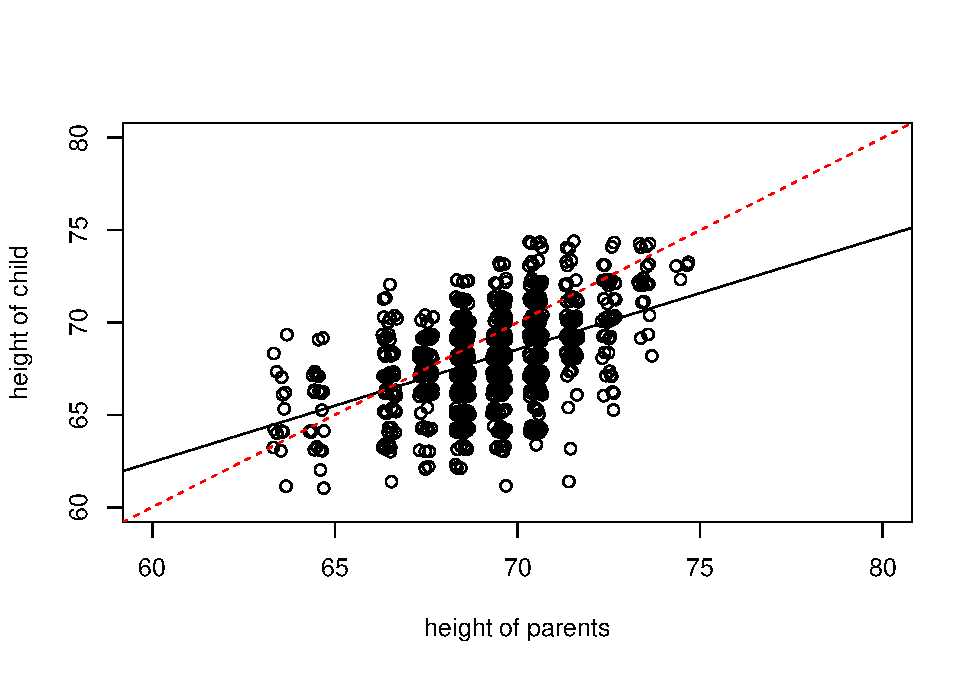
\includegraphics{RegressModelDataCamp_files/figure-latex/unnamed-chunk-3-1.pdf}

\begin{Shaded}
\begin{Highlighting}[]
\KeywordTok{summary}\NormalTok{(}\KeywordTok{lm}\NormalTok{(heights}\OperatorTok{$}\NormalTok{child_ht}\OperatorTok{~}\NormalTok{heights}\OperatorTok{$}\NormalTok{parent_ht))}
\end{Highlighting}
\end{Shaded}

\begin{verbatim}

Call:
lm(formula = heights$child_ht ~ heights$parent_ht)

Residuals:
    Min      1Q  Median      3Q     Max 
-8.2577 -1.4280  0.1323  1.5720  5.7918 

Coefficients:
                  Estimate Std. Error t value Pr(>|t|)    
(Intercept)       25.84856    2.69009   9.609   <2e-16 ***
heights$parent_ht  0.60992    0.03882  15.710   <2e-16 ***
---
Signif. codes:  0 '***' 0.001 '**' 0.01 '*' 0.05 '.' 0.1 ' ' 1

Residual standard error: 2.26 on 926 degrees of freedom
Multiple R-squared:  0.2104,    Adjusted R-squared:  0.2096 
F-statistic: 246.8 on 1 and 926 DF,  p-value: < 2.2e-16
\end{verbatim}

\chapter{Regression and the Normal
Distribution}\label{regression-and-the-normal-distribution}

\textbf{Chapter description}

Regression analysis is a statistical method that is widely used in many
fields of study, with actuarial science being no exception. This chapter
introduces the role of the normal distribution in regression and the use
of logarithmic transformations in specifying regression relationships.

\section{Fitting a normal
distribution}\label{fitting-a-normal-distribution}

\begin{center}\rule{0.5\linewidth}{\linethickness}\end{center}

In this section, you learn how to:

\begin{itemize}
\tightlist
\item
  Calculate and interpret two basic summary statistics
\item
  Fit a data set to a normal curve
\item
  Calculate probabilities under a standard normal curve
\end{itemize}

\begin{center}\rule{0.5\linewidth}{\linethickness}\end{center}

\subsection{Video}\label{video}

\subsubsection*{Video Overhead Details}\label{video-overhead-details}
\addcontentsline{toc}{subsubsection}{Video Overhead Details}

Show Overhead A Details. Description of the data

\hypertarget{toggleOver1.1A}{}
To illustrate a data set that can be analyzed using regression methods,
we consider some data included in Galton's 1885 paper. These data
include the heights of 928 adult children (child\_ht), together with an
index of their parents' height (parent\_ht). Here, all female heights
were multiplied by 1.08, and the index was created by taking the average
of the father's height and rescaled mother's height. Galton was aware
that the parents' and the adult child's height could each be adequately
approximated by a normal curve. In developing regression analysis, he
provided a single model for the joint distribution of heights.

\begin{Shaded}
\begin{Highlighting}[]
\NormalTok{heights <-}\StringTok{ }\KeywordTok{read.csv}\NormalTok{(}\StringTok{"CSVData}\CharTok{\textbackslash{}\textbackslash{}}\StringTok{galton_height.csv"}\NormalTok{, }\DataTypeTok{header =} \OtherTok{TRUE}\NormalTok{)}
\CommentTok{#heights <- read.csv("https://assets.datacamp.com/production/repositories/2610/datasets/c85ede6c205d22049e766bd08956b225c576255b/galton_height.csv", header = TRUE)}
\KeywordTok{plot}\NormalTok{(}\KeywordTok{jitter}\NormalTok{(heights}\OperatorTok{$}\NormalTok{parent_ht),}\KeywordTok{jitter}\NormalTok{(heights}\OperatorTok{$}\NormalTok{child_ht), }\DataTypeTok{ylim =} \KeywordTok{c}\NormalTok{(}\DecValTok{60}\NormalTok{,}\DecValTok{80}\NormalTok{), }\DataTypeTok{xlim =} \KeywordTok{c}\NormalTok{(}\DecValTok{60}\NormalTok{,}\DecValTok{80}\NormalTok{),}
     \DataTypeTok{ylab =} \StringTok{"height of child"}\NormalTok{, }\DataTypeTok{xlab =} \StringTok{"height of parents"}\NormalTok{)}
\KeywordTok{abline}\NormalTok{(}\KeywordTok{lm}\NormalTok{(heights}\OperatorTok{$}\NormalTok{child_ht}\OperatorTok{~}\NormalTok{heights}\OperatorTok{$}\NormalTok{parent_ht))}
\KeywordTok{abline}\NormalTok{(}\DecValTok{0}\NormalTok{,}\DecValTok{1}\NormalTok{,}\DataTypeTok{col =} \StringTok{"red"}\NormalTok{)}
\end{Highlighting}
\end{Shaded}

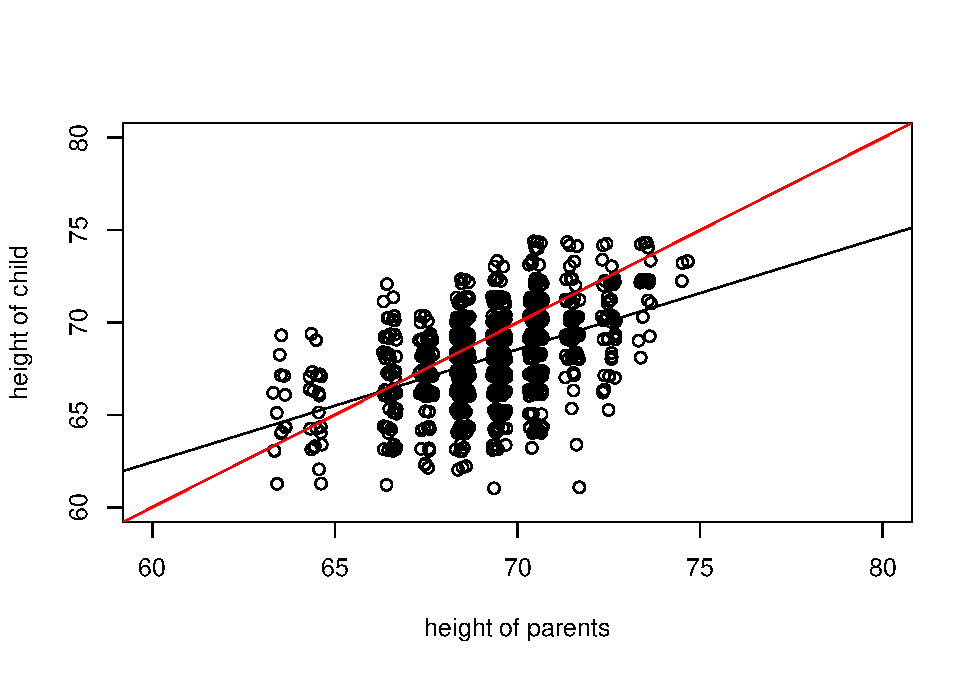
\includegraphics{RegressModelDataCamp_files/figure-latex/unnamed-chunk-4-1.pdf}

Show Overhead B Details. Read and examine data structure

\hypertarget{toggleOver1.1B}{}
The data has already been read into a dataset called \texttt{heights}.
Examine the \emph{structure} of the data with the function
\href{https://www.rdocumentation.org/packages/utils/versions/3.5.0/topics/str/}{str()}
and use the
\href{https://www.rdocumentation.org/packages/utils/versions/3.5.0/topics/head/}{head()}
command to looks at the first few records.

\begin{Shaded}
\begin{Highlighting}[]
\NormalTok{heights <-}\StringTok{ }\KeywordTok{read.csv}\NormalTok{(}\StringTok{"CSVData}\CharTok{\textbackslash{}\textbackslash{}}\StringTok{galton_height.csv"}\NormalTok{,}\DataTypeTok{header =} \OtherTok{TRUE}\NormalTok{)}
\CommentTok{#heights <- read.csv("https://assets.datacamp.com/production/repositories/2610/datasets/c85ede6c205d22049e766bd08956b225c576255b/galton_height.csv", header = TRUE)}
\KeywordTok{str}\NormalTok{(heights)}
\KeywordTok{head}\NormalTok{(heights)}
\end{Highlighting}
\end{Shaded}

\begin{verbatim}
'data.frame':   928 obs. of  2 variables:
 $ child_ht : num  72.2 73.2 73.2 73.2 68.2 ...
 $ parent_ht: num  74.5 74.5 74.5 74.5 73.5 73.5 73.5 73.5 73.5 73.5 ...
  child_ht parent_ht
1     72.2      74.5
2     73.2      74.5
3     73.2      74.5
4     73.2      74.5
5     68.2      73.5
6     69.2      73.5
\end{verbatim}

Show Overhead C Details. Summary stats for parents' height

\hypertarget{toggleOver1.1C}{}
Next, examine the distribution of the child's height and then examine
the distribution of the parents height.

\begin{Shaded}
\begin{Highlighting}[]
\NormalTok{ht_par <-}\StringTok{ }\NormalTok{heights}\OperatorTok{$}\NormalTok{parent_ht}
\KeywordTok{hist}\NormalTok{(ht_par)}
\end{Highlighting}
\end{Shaded}

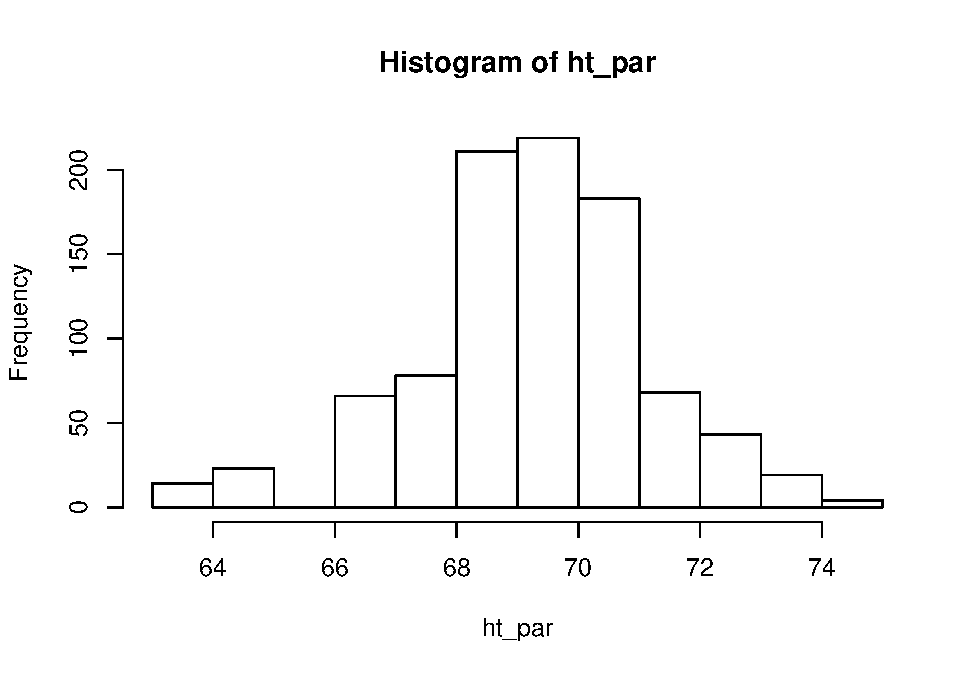
\includegraphics{RegressModelDataCamp_files/figure-latex/unnamed-chunk-6-1.pdf}

\begin{Shaded}
\begin{Highlighting}[]
\KeywordTok{mean}\NormalTok{(ht_par)}
\KeywordTok{sd}\NormalTok{(ht_par)}
\end{Highlighting}
\end{Shaded}

\begin{verbatim}
[1] 69.26293
[1] 1.912274
\end{verbatim}

Show Overhead D. Fit a normal curve to parents' height details

\hypertarget{toggleOver1.1D}{}
\begin{Shaded}
\begin{Highlighting}[]
\NormalTok{(mparent <-}\StringTok{ }\KeywordTok{mean}\NormalTok{(ht_par))}
\NormalTok{(sdparent <-}\StringTok{ }\KeywordTok{sd}\NormalTok{(ht_par))}
\NormalTok{x <-}\StringTok{ }\KeywordTok{seq}\NormalTok{(}\DecValTok{60}\NormalTok{, }\DecValTok{80}\NormalTok{,}\DataTypeTok{by =} \FloatTok{0.1}\NormalTok{)}
\KeywordTok{hist}\NormalTok{(ht_par, }\DataTypeTok{freq =} \OtherTok{FALSE}\NormalTok{)}
\KeywordTok{lines}\NormalTok{(x, }\KeywordTok{dnorm}\NormalTok{(x, }\DataTypeTok{mean =}\NormalTok{ mparent, }\DataTypeTok{sd =}\NormalTok{ sdparent), }\DataTypeTok{col =} \StringTok{"blue"}\NormalTok{)}
\end{Highlighting}
\end{Shaded}

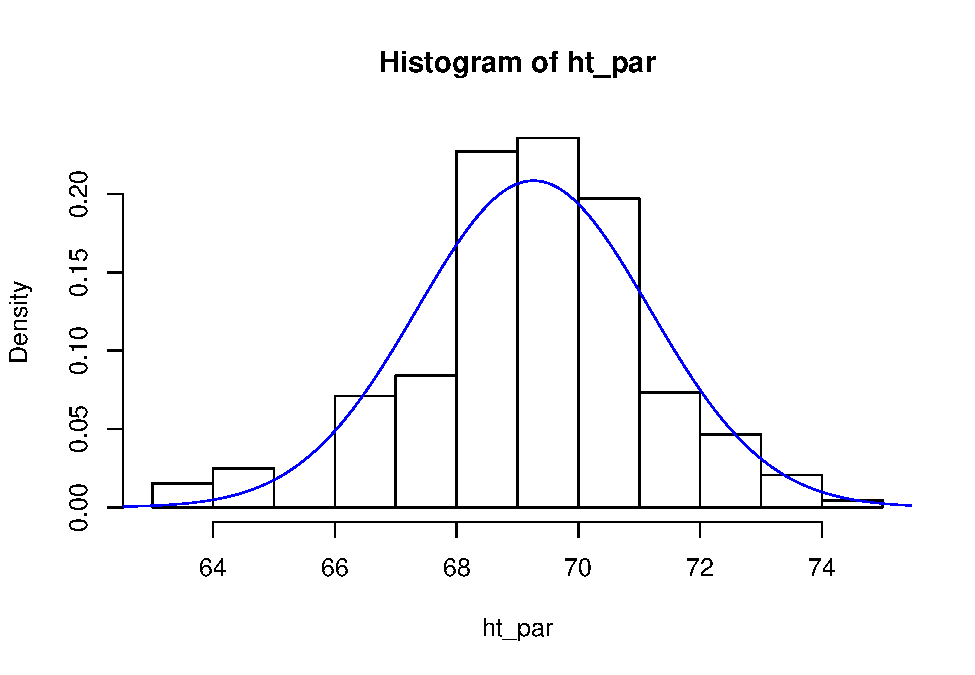
\includegraphics{RegressModelDataCamp_files/figure-latex/unnamed-chunk-7-1.pdf}

\begin{verbatim}
[1] 69.26293
[1] 1.912274
\end{verbatim}

Show Overhead E Details. Use the normal approximation to determine the
probability of the height of tall parents

\hypertarget{toggleOver1.1E}{}
\begin{Shaded}
\begin{Highlighting}[]
\NormalTok{TallHeight <-}\StringTok{ }\DecValTok{72}
\KeywordTok{pnorm}\NormalTok{(TallHeight, }\DataTypeTok{mean =}\NormalTok{ mparent, }\DataTypeTok{sd =}\NormalTok{ sdparent)}
\KeywordTok{pnorm}\NormalTok{(}\DecValTok{72}\NormalTok{, }\DataTypeTok{mean =} \KeywordTok{mean}\NormalTok{(ht_par), }\DataTypeTok{sd =} \KeywordTok{sd}\NormalTok{(ht_par))}
\NormalTok{(StdUnitsTallHeight <-}\StringTok{ }\NormalTok{(TallHeight }\OperatorTok{-}\StringTok{ }\NormalTok{mparent)}\OperatorTok{/}\NormalTok{sdparent)}
\KeywordTok{pnorm}\NormalTok{(StdUnitsTallHeight, }\DataTypeTok{mean =} \DecValTok{0}\NormalTok{, }\DataTypeTok{sd =} \DecValTok{1}\NormalTok{)}
\end{Highlighting}
\end{Shaded}

\begin{verbatim}
[1] 0.9238302
[1] 0.9238302
[1] 1.431317
[1] 0.9238302
\end{verbatim}

\subsection{Exercise. Fitting Galton's height
data}\label{exercise.-fitting-galtons-height-data}

\textbf{Assignment Text}

The Galton data has already been read into a dataframe called
\texttt{heights}. These data include the heights of 928 adult children
\texttt{child\_ht}, together with an index of their parents' height
\texttt{parent\_ht}. The video explored the distribution of the parents'
height; in this assignment, we investigate the distribution of the
heights of the adult children.

\textbf{Instructions}

\begin{itemize}
\tightlist
\item
  Define the height of an adult child as a global variable
\item
  Use the function
  \href{https://www.rdocumentation.org/packages/base/versions/3.5.0/topics/mean/}{mean()}
  to calculate the mean and the function
  \href{https://www.rdocumentation.org/packages/base/versions/3.5.0/topics/sd/}{sd()}
  to calculate the standard deviation
\item
  Use the normal approximation and the function
  \href{https://www.rdocumentation.org/packages/stats/versions/3.5.0/topics/Normal/}{pnorm()}
  determine the probability that an adult child's height is less than 72
  inches
\end{itemize}

\textbf{Hint.} Remember that we can reference a variable, say
\texttt{var}, from a data set such as \texttt{heights}, as
\texttt{heights\$var}.

eyJsYW5ndWFnZSI6InIiLCJwcmVfZXhlcmNpc2VfY29kZSI6IiNoZWlnaHRzIDwtIHJlYWQuY3N2KFwiQ1NWRGF0YVxcXFxnYWx0b25faGVpZ2h0LmNzdlwiLGhlYWRlciA9IFRSVUUpXG5oZWlnaHRzIDwtIHJlYWQuY3N2KFwiaHR0cHM6Ly9hc3NldHMuZGF0YWNhbXAuY29tL3Byb2R1Y3Rpb24vcmVwb3NpdG9yaWVzLzI2MTAvZGF0YXNldHMvYzg1ZWRlNmMyMDVkMjIwNDllNzY2YmQwODk1NmIyMjVjNTc2MjU1Yi9nYWx0b25faGVpZ2h0LmNzdlwiLCBoZWFkZXIgPSBUUlVFKSIsInNhbXBsZSI6IiNEZWZpbmUgdGhlIGdsb2JhbCB2YXJpYWJsZVxuaHRfY2hpbGQgPC0gX19fXG5cbiNDYWxjdWxhdGUgdGhlIG1lYW4gaGVpZ2h0XG5tY2hpbGQgPC0gX19fXG5tY2hpbGRcblxuI0NhbGN1bGF0ZSB0aGUgc3RhbmRhcmQgZGV2aWF0aW9uIG9mIGhlaWdodHNcbnNkY2hpbGQgPC0gX19fXG5zZGNoaWxkXG5cbiNEZXRlcm1pbmUgdGhlIHByb2JhYmlsaXR5IHRoYXQgdGhlIGhlaWdodCBpcyBsZXNzIHRoYW4gNzJcbnByPV9fXyg3MiwgbWVhbj1tY2hpbGQsIHNkPXNkY2hpbGQpIiwic29sdXRpb24iOiIjIFNvbHV0aW9uXG5odF9jaGlsZCA8LSBoZWlnaHRzJGNoaWxkX2h0XG5tY2hpbGQgPC0gbWVhbihodF9jaGlsZClcbnNkY2hpbGQgPC0gc2QoaHRfY2hpbGQpXG5wcj1wbm9ybSg3MiwgbWVhbiA9IG1jaGlsZCwgc2QgPSBzZGNoaWxkKSIsInNjdCI6ImV4KCkgJT4lIGNoZWNrX29iamVjdChcImh0X2NoaWxkXCIsdW5kZWZpbmVkX21zZz1cIk1ha2Ugc3VyZSB5b3UgYXNzaWduIHRoZSBjaGlsZHJlbidzIGhpZ2h0IHRvIGh0X2NoaWxkXCIpICU+JSBjaGVja19lcXVhbChpbmNvcnJlY3RfbXNnPVwiUmVtZW1iZXIgdGhhdCBpbiBvcmRlciB0byBjYWxsIGEgc3BlY2lmaWMgY29sdW1uIGZyb20gYSBkYXRhZnJhbWUsIHVzZSB0aGUgJCBvcGVyYXRvclwiKVxuZXgoKSAlPiUgY2hlY2tfb2JqZWN0KFwibWNoaWxkXCIpICAlPiUgY2hlY2tfZXF1YWwoKVxuZXgoKSAlPiUgY2hlY2tfb2JqZWN0KFwic2RjaGlsZFwiKSAlPiUgY2hlY2tfZXF1YWwoKVxuZXgoKSAlPiUgY2hlY2tfb2JqZWN0KFwicHJcIikgJT4lIGNoZWNrX2VxdWFsKClcbnN1Y2Nlc3NfbXNnKFwiRXhjZWxsZW50ISBXaXRoIHRoaXMgcHJvY2VkdXJlLCB5b3UgY2FuIG5vdyBjYWxjdWxhdGUgcHJvYmFiaWxpdGllcyBmb3IgYW55IGRpc3RyaWJ1dGlvbiB1c2luZyBhIG5vcm1hbCBjdXJ2ZSBhcHByb3hpbWF0aW9uLlwiKSJ9

\subsection{Exercise. Visualizing child's height
distribution}\label{exercise.-visualizing-childs-height-distribution}

\textbf{Assignment Text}

As in the prior exercise, from the Galton dataset \texttt{heights}, the
heights of 928 adult children have been used to create a global variable
called \texttt{ht\_child}. We also have basic summary statistics, the
mean height \texttt{mchild} and the standard deviation of heights in
\texttt{sdchild}. In this exercise, we explore the fit of the normal
curve to this distribution.

\textbf{Instructions}

\begin{itemize}
\tightlist
\item
  To visualize the distribution, use the function
  \href{https://www.rdocumentation.org/packages/graphics/versions/3.5.0/topics/hist/}{hist()}
  to calculate the histogram. Use the \texttt{freq\ =\ FALSE} option to
  give a histogram with proportions instead of counts.
\item
  Use the function
  \href{https://www.rdocumentation.org/packages/base/versions/3.5.0/topics/seq}{seq()}
  to determine a sequence that can be used for plotting. Then, with the
  function
  \href{https://www.rdocumentation.org/packages/graphics/versions/3.5.0/topics/lines/}{lines()},
  superimpose a normal curve on the histogram
\item
  Determine the probability that a child's height is greater than 72
  inches
\end{itemize}

\textbf{Hint 1.} Use the function
\href{https://www.rdocumentation.org/packages/stats/versions/3.5.0/topics/Normal/}{dnorm()}
to calculate the normal density, similar to the cumulative probabilites
that you calculated using
\href{https://www.rdocumentation.org/packages/stats/versions/3.5.0/topics/Normal/}{pnorm()}

\textbf{Hint 2.} To calculate probabilities greater that an amount,
simply use 1 minus the cumulative probability

\textbf{Pre-exercise code}

eyJsYW5ndWFnZSI6InIiLCJwcmVfZXhlcmNpc2VfY29kZSI6IiNoZWlnaHRzIDwtIHJlYWQuY3N2KFwiQ1NWRGF0YVxcXFxnYWx0b25faGVpZ2h0LmNzdlwiLGhlYWRlciA9IFRSVUUpXG5oZWlnaHRzIDwtIHJlYWQuY3N2KFwiaHR0cHM6Ly9hc3NldHMuZGF0YWNhbXAuY29tL3Byb2R1Y3Rpb24vcmVwb3NpdG9yaWVzLzI2MTAvZGF0YXNldHMvYzg1ZWRlNmMyMDVkMjIwNDllNzY2YmQwODk1NmIyMjVjNTc2MjU1Yi9nYWx0b25faGVpZ2h0LmNzdlwiLCBoZWFkZXIgPSBUUlVFKVxuaHRfY2hpbGQgPC0gaGVpZ2h0cyRjaGlsZF9odFxubWNoaWxkIDwtIG1lYW4oaHRfY2hpbGQpXG5zZGNoaWxkIDwtIHNkKGh0X2NoaWxkKSIsInNhbXBsZSI6IiNWaXN1YWxpemUgdGhlIERpc3RyaWJ1dGlvblxuX19fKF9fXywgZnJlcSA9IEZBTFNFKVxuXG4jRGV0ZXJtaW5lIGEgc2VxdWVuY2UuIFRoZW4sIGdyYXBoIGEgaGlzdG9ncmFtIHdpdGggYSBub3JtYWwgY3VydmUgc3VwZXJpbXBvc2VkXG54IDwtIHNlcSg2MCwgODAsYnkgPSAwLjEpXG5fX18oeCwgZG5vcm0oeCxtZWFuID0gbWNoaWxkLCBzZCA9IHNkY2hpbGQpLCBjb2wgPSBcImJsdWVcIilcblxuIyBEZXRlcm1pbmUgdGhlIHByb2JhYmlsaXR5IHRoYXQgYSBjaGlsZCdzIGhlaWdodCBpcyBncmVhdGVyIHRoYW4gNzJcbnByb2IgPC0gMSAtIFxucHJvYiIsInNvbHV0aW9uIjoiaGlzdChodF9jaGlsZCwgZnJlcSA9IEZBTFNFKVxueCA8LSBzZXEoNjAsIDgwLGJ5ID0gMC4xKVxubGluZXMoeCwgZG5vcm0oeCwgbWVhbiA9IG1jaGlsZCwgc2QgPSBzZGNoaWxkKSwgY29sID0gXCJibHVlXCIpXG5wcm9iIDwtIDEgLSBwbm9ybSg3MiwgbWVhbiA9IG1jaGlsZCAsIHNkID0gc2RjaGlsZClcbnByb2IiLCJzY3QiOiJleCgpICU+JSBjaGVja19mdW5jdGlvbihcImhpc3RcIixub3RfY2FsbGVkX21zZz1cIlVzZSB0aGUgaGlzdCBjb21tYW5kIHRvIGNyZWF0ZSBhIGhpc3RvZ3JhbSBvZiB0aGUgY2hpbGRyZW4ncyBoZWlnaHRzLlwiKSAlPiUgY2hlY2tfYXJnKFwieFwiKSAlPiUgY2hlY2tfZXF1YWwoaW5jb3JyZWN0X21zZz1cIk1ha2Ugc3VyZSB0byBjcmVhdGUgYSBoaXN0b2dyYW0gb2YgdGhlIGNoaWxkcmVuJ3MgaGVpZ2h0cy5cIilcbmV4KCkgJT4lIGNoZWNrX2Z1bmN0aW9uKFwibGluZXNcIixub3RfY2FsbGVkX21zZz1cIlBsZWFzZSB1c2UgdGhlIGxpbmVzIGZ1bmN0aW9uIHRvIG92ZXJsYXkgYSBub3JtYWwgY3VydmUgb24geW91ciBoaXN0b2dyYW1cIilcbmV4KCkgJT4lIGNoZWNrX29iamVjdChcInByb2JcIiwgdW5kZWZpbmVkX21zZz1cIk1ha2Ugc3VyZSB0byBhc3NpZ24gdGhlIHByb2JhYmlsaXR5IG9mIGEgY2hpbGQncyBoZWlnaHQgYmVpbmcgZ3JlYXRlciB0aGFuIDcyIGluY2hlcyB0byBwcm9iLlwiKSAlPiUgY2hlY2tfZXF1YWwoaW5jb3JyZWN0X21zZz1cIk1ha2Ugc3VyZSB0byBmaW5kIHRoZSBwcm9iYWJpbGl0eSBvZiBhIGNoaWxkJ3MgaGVpZ2h0IGJlaW5nIEdSRUFURVIgdGhhbiA3MiBpbmNoZXMuXCIpXG5zdWNjZXNzX21zZyhcIkV4Y2VsbGVudCEgVmlzdWFsaXppbmcgYSBkaXN0cmlidXRpb24sIGVzcGVjaWFsbHkgd2l0aCByZWZlcmVuY2UgdG8gYSBub3JtYWwsIGlzIGltcG9ydGFudCBmb3IgY29tbXVuaWNhdGluZyByZXN1bHRzIG9mIHlvdXIgYW5hbHlzaXMuXCIpIn0=

\section{Visualizing distributions}\label{visualizing-distributions}

\begin{center}\rule{0.5\linewidth}{\linethickness}\end{center}

In this section, you learn how to:

\begin{itemize}
\tightlist
\item
  Calculate and interpret distributions using histograms
\item
  Calculate and interpret distributions using density plots
\end{itemize}

\begin{center}\rule{0.5\linewidth}{\linethickness}\end{center}

\subsection{Video}\label{video-1}

\subsubsection*{Video Overhead Details}\label{video-overhead-details-1}
\addcontentsline{toc}{subsubsection}{Video Overhead Details}

Show Overhead Details. Data description

\hypertarget{toggleOver1.2}{}
\begin{center}\rule{0.5\linewidth}{\linethickness}\end{center}

For our first look at an insurance data set, we consider data from
Rempala and Derrig (2005). They considered claims arising from
automobile bodily injury insurance coverages. These are amounts incurred
for outpatient medical treatments that arise from automobile accidents,
typically sprains, broken collarbones and the like. The data consists of
a sample of 272 claims from Massachusetts that were closed in 2001 (by
``closed,'' we mean that the claim is settled and no additional
liabilities can arise from the same accident). Rempala and Derrig were
interested in developing procedures for handling mixtures of ``typical''
claims and others from providers who reported claims fraudulently. For
this sample, we consider only those typical claims, ignoring the
potentially fraudulent ones.

\begin{Shaded}
\begin{Highlighting}[]
\CommentTok{# Reformat Data Set}
\NormalTok{injury <-}\StringTok{ }\KeywordTok{read.csv}\NormalTok{(}\StringTok{"CSVData}\CharTok{\textbackslash{}\textbackslash{}}\StringTok{MassBodilyInjury.csv"}\NormalTok{,}\DataTypeTok{header =} \OtherTok{TRUE}\NormalTok{)}
\KeywordTok{str}\NormalTok{(injury)}
\KeywordTok{head}\NormalTok{(injury)}
\CommentTok{#  PICK THE SUBSET OF THE DATA CORRESPONDING TO PROVIDER A}
\NormalTok{injury2 <-}\StringTok{ }\KeywordTok{subset}\NormalTok{(injury, providerA }\OperatorTok{!}\StringTok{ }\ErrorTok{=}\StringTok{ }\DecValTok{0}\NormalTok{ )}
\NormalTok{injury2}\OperatorTok{$}\NormalTok{claims <-}\StringTok{ }\DecValTok{1000}\OperatorTok{*}\NormalTok{injury2}\OperatorTok{$}\NormalTok{claims}
\NormalTok{injury2}\OperatorTok{$}\NormalTok{logclaims <-}\StringTok{ }\KeywordTok{log}\NormalTok{(injury2}\OperatorTok{$}\NormalTok{claims)}
\NormalTok{injury3 <-}\StringTok{ }\NormalTok{injury2[}\KeywordTok{c}\NormalTok{(}\StringTok{"claims"}\NormalTok{,}\StringTok{"logclaims"}\NormalTok{)]}
\CommentTok{#write.csv(injury3,"CSVData\textbackslash{}\textbackslash{}MassBI.csv",row.names = FALSE)}
\end{Highlighting}
\end{Shaded}

Show Overhead A Details. Bring in Data, Introduce Logarithmic Claims

\hypertarget{toggleOver1.2A}{}
\begin{Shaded}
\begin{Highlighting}[]
\NormalTok{injury <-}\StringTok{ }\KeywordTok{read.csv}\NormalTok{(}\StringTok{"CSVData}\CharTok{\textbackslash{}\textbackslash{}}\StringTok{MassBI.csv"}\NormalTok{,}\DataTypeTok{header =} \OtherTok{TRUE}\NormalTok{)}
\CommentTok{#  CHECK THE NAMES, DIMENSION IN THE FILE AND LIST THE FIRST 8 OBSERVATIONS  ;}
\KeywordTok{str}\NormalTok{(injury)}
\KeywordTok{head}\NormalTok{(injury)}
\KeywordTok{attach}\NormalTok{(injury)}
\NormalTok{claims <-}\StringTok{ }\NormalTok{injury}\OperatorTok{$}\NormalTok{claims}
\KeywordTok{par}\NormalTok{(}\DataTypeTok{mfrow =} \KeywordTok{c}\NormalTok{(}\DecValTok{1}\NormalTok{, }\DecValTok{2}\NormalTok{))}
\KeywordTok{hist}\NormalTok{(claims)}
\KeywordTok{hist}\NormalTok{(logclaims)}
\end{Highlighting}
\end{Shaded}

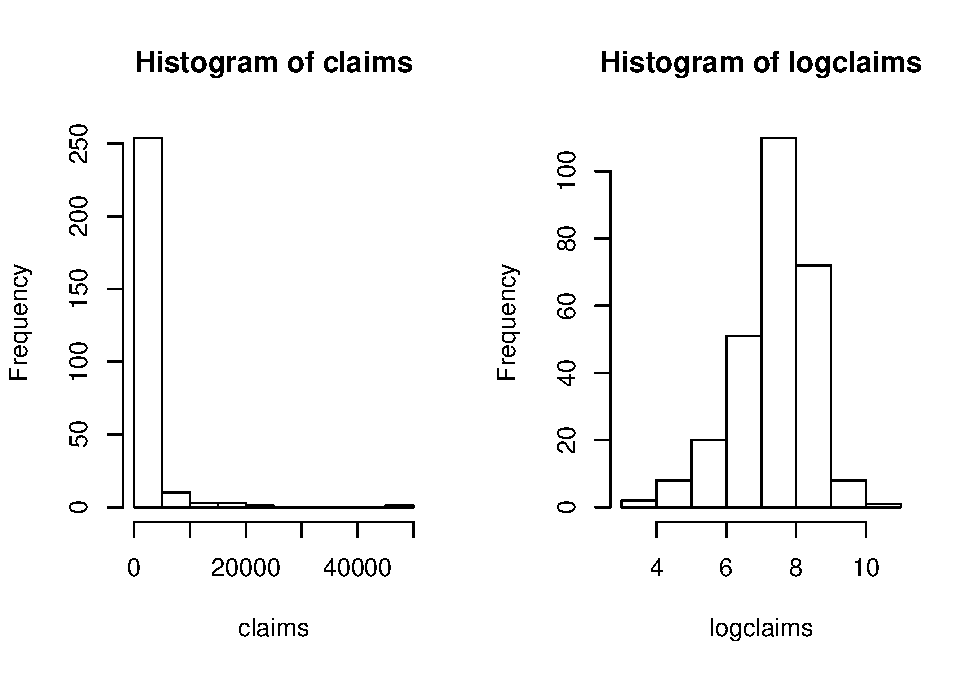
\includegraphics{RegressModelDataCamp_files/figure-latex/unnamed-chunk-18-1.pdf}

\begin{verbatim}
'data.frame':   272 obs. of  2 variables:
 $ claims   : int  45 47 70 75 77 92 117 117 140 145 ...
 $ logclaims: num  3.81 3.85 4.25 4.32 4.34 ...
  claims logclaims
1     45  3.806662
2     47  3.850148
3     70  4.248495
4     75  4.317488
5     77  4.343805
6     92  4.521789
\end{verbatim}

Show Overhead B Details. Show how to get a finer grid for histograms

\hypertarget{toggleOver1.2B}{}
\begin{Shaded}
\begin{Highlighting}[]
\KeywordTok{par}\NormalTok{(}\DataTypeTok{mfrow =} \KeywordTok{c}\NormalTok{(}\DecValTok{1}\NormalTok{, }\DecValTok{2}\NormalTok{))}
\KeywordTok{hist}\NormalTok{(logclaims)}
\KeywordTok{hist}\NormalTok{(logclaims,}\DataTypeTok{breaks =} \DecValTok{15}\NormalTok{)}
\end{Highlighting}
\end{Shaded}

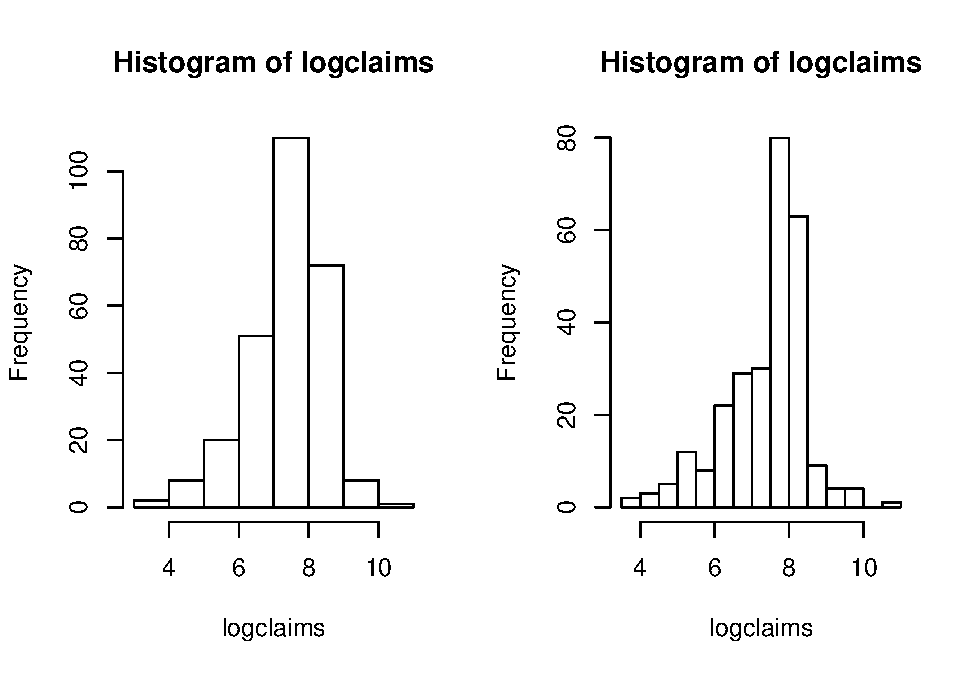
\includegraphics{RegressModelDataCamp_files/figure-latex/unnamed-chunk-19-1.pdf}

Show Overhead C Details. Introduce the density plot

\hypertarget{toggleOver1.2C}{}
\begin{Shaded}
\begin{Highlighting}[]
\KeywordTok{par}\NormalTok{(}\DataTypeTok{mfrow =} \KeywordTok{c}\NormalTok{(}\DecValTok{1}\NormalTok{, }\DecValTok{2}\NormalTok{))}
\KeywordTok{plot}\NormalTok{(}\KeywordTok{density}\NormalTok{(logclaims))}
\KeywordTok{hist}\NormalTok{(logclaims, }\DataTypeTok{breaks =} \DecValTok{15}\NormalTok{,}\DataTypeTok{freq =} \OtherTok{FALSE}\NormalTok{)}
\KeywordTok{lines}\NormalTok{(}\KeywordTok{density}\NormalTok{(logclaims))}
\end{Highlighting}
\end{Shaded}

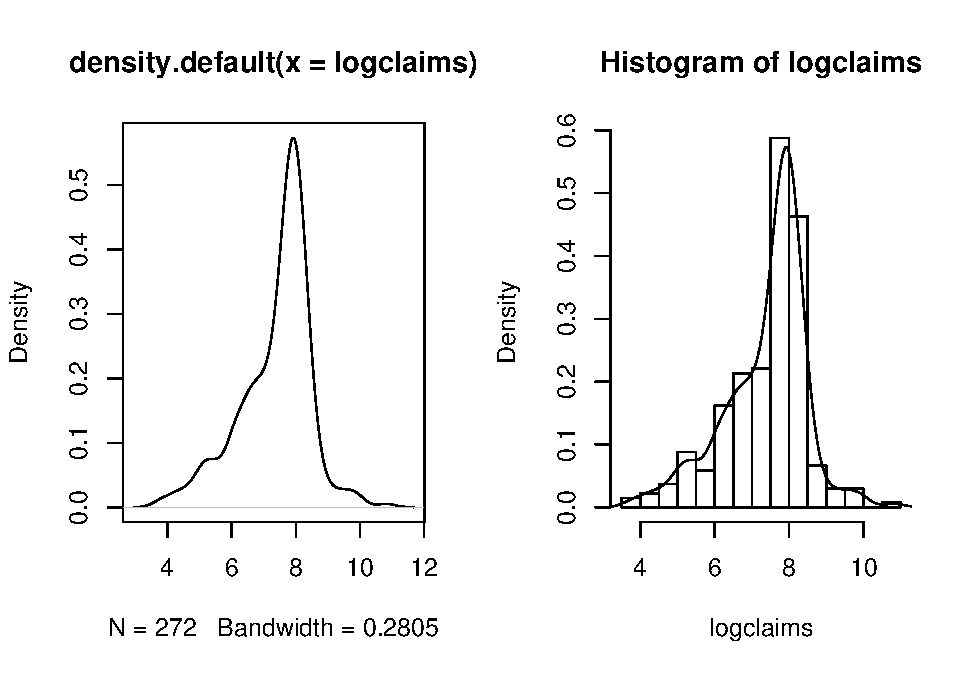
\includegraphics{RegressModelDataCamp_files/figure-latex/unnamed-chunk-20-1.pdf}

\subsection{Exercise. Visualizing bodily injury claims with density
plots}\label{exercise.-visualizing-bodily-injury-claims-with-density-plots}

\textbf{Assignment Text}

In the prior video, you learned about the Massachusetts bodily injury
dataset. This dataframe, \texttt{injury}, has been read in and the
global variable \texttt{claims} has been created. This assignment
reviews the
\href{https://www.rdocumentation.org/packages/graphics/versions/3.5.0/topics/hist/}{hist()}
function for visualizing distributions and allows you to explore density
plotting, a smoothed version of the histogram.

\textbf{Instructions}

\begin{itemize}
\tightlist
\item
  Use the function
  \href{https://www.rdocumentation.org/packages/base/versions/3.5.0/topics/log/}{log()}
  to create the logarithmic version of the claims variable
\item
  Calculate a histogram of logarithmic with 40 bins using an option in
  the
  \href{https://www.rdocumentation.org/packages/graphics/versions/3.5.0/topics/hist/}{hist()}
  function, \texttt{breaks\ =}.
\item
  Create a density plot of logarithmic claims using the functions
  \href{https://www.rdocumentation.org/packages/graphics/versions/3.5.0/topics/plot/}{plot()}
  and
  \href{https://www.rdocumentation.org/packages/stats/versions/3.5.0/topics/density/}{density()}.
\item
  Repeat the density plot, this time using a more refined bandwidth
  equal to 0.03. Use an option in the
  \href{https://www.rdocumentation.org/packages/stats/versions/3.5.0/topics/density/}{density()}
  function, \texttt{bw\ =}.
\end{itemize}

eyJsYW5ndWFnZSI6InIiLCJwcmVfZXhlcmNpc2VfY29kZSI6IiNpbmp1cnkgPC0gcmVhZC5jc3YoXCJDU1ZEYXRhXFxcXE1hc3NCSS5jc3ZcIixoZWFkZXIgPSBUUlVFKVxuaW5qdXJ5IDwtIHJlYWQuY3N2KFwiaHR0cHM6Ly9hc3NldHMuZGF0YWNhbXAuY29tL3Byb2R1Y3Rpb24vcmVwb3NpdG9yaWVzLzI2MTAvZGF0YXNldHMvOGNjYTE5ZDA1MDNmY2Y2ZTlkMzBkOWNiOTEyZGU1YmE5NWVjYjljMS9NYXNzQkkuY3N2XCIsIGhlYWRlciA9IFRSVUUpXG5jbGFpbXMgPC0gaW5qdXJ5JGNsYWltcyIsInNhbXBsZSI6IiNDcmVhdGUgdGhlIGxvZ2FyaXRobWljIGNsYWltcyB2YXJpYWJsZVxubG9nY2xhaW1zIDwtIF9fX1xuXG4jQ3JlYXRlIGEgaGlzdG9ncmFtIHVzaW5zIDQwIGJpbnNcbl9fXyhsb2djbGFpbXMsIGJyZWFrcyA9IDQwLGZyZXEgPSBGQUxTRSlcbmJveCgpXG5cbiMgQ3JlYXRlIGEgZGVuc2l0eSBwbG90IG9mIGxvZ2FyaXRobWljIGNsYWltc1xucGxvdChfX18obG9nY2xhaW1zKSlcblxuIyBDcmVhdGUgYSBkZW5zaXR5IHBsb3Qgb2YgbG9nYXJpdGhtaWMgY2xhaW1zIHdpdGggYSBiYW5kd2lkdGggb2YgMC4wM1xuX19fIiwic29sdXRpb24iOiJsb2djbGFpbXMgPC0gbG9nKGNsYWltcylcbmhpc3QobG9nY2xhaW1zICwgYnJlYWtzID0gNDAsZnJlcSA9IEZBTFNFKVxuYm94KClcbnBsb3QoZGVuc2l0eShsb2djbGFpbXMpKVxucGxvdChkZW5zaXR5KGxvZ2NsYWltcywgYncgPSAwLjAzKSkiLCJzY3QiOiJleCgpICU+JSBjaGVja19vYmplY3QoXCJsb2djbGFpbXNcIikgJT4lIGNoZWNrX2VxdWFsKGluY29ycmVjdF9tc2cgPSBcIllvdSBtYWRlIGFuIGVycm9yIGluIHRoZSBkZWZpbml0aW9uIG9mIHRoZSBsb2dhcml0aG1pYyBjbGFpbXMuIENoZWNrIG91dCB0aGUgZGVmaW5pdGlvbiBvZiB0aGUgbG9nKCkgZnVuY3Rpb24uXCIpXG5leCgpICU+JSBjaGVja19mdW5jdGlvbihcImhpc3RcIixub3RfY2FsbGVkX21zZz1cIk1ha2Ugc3VyZSB0byB1c2UgYGhpc3RgIHRvIGNyZWF0ZSBhIGhpc3RvZ3JhbS5cIikgJT4lIHtcbiAgY2hlY2tfYXJnKC4sIFwieFwiKSAlPiUgY2hlY2tfZXF1YWwoaW5jb3JyZWN0X21zZz1cIlBsZWFzZSBjcmVhdGUgYSBoaXN0b2dyYW0gb2YgbG9nY2xhaW1zLlwiKVxuICBjaGVja19hcmcoLiwgXCJmcmVxXCIpICU+JSBjaGVja19lcXVhbChpbmNvcnJlY3RfbXNnPVwiUGxlYXNlIGNyZWF0ZSBhIGRlbnNpdHkgaGlzdG9ncmFtIGluc3RlYWQgb2YgYSBmcmVxdWVuY3kgaGlzdG9ncmFtLlwiKVxufVxuZXgoKSAlPiUgY2hlY2tfZnVuY3Rpb24oXCJwbG90XCIsaW5kZXg9MSkgJT4lIGNoZWNrX2FyZyhcInhcIikgJT4lIGNoZWNrX2VxdWFsKGluY29ycmVjdF9tc2c9XCJVc2UgdGhlIGRlbnNpdHkgZnVuY3Rpb24gdG8gcGxvdCB0aGUgZGVuc2l0eSBvZiBsb2djbGFpbXMuXCIpXG5leCgpICU+JSBjaGVja19mdW5jdGlvbihcInBsb3RcIixpbmRleD0yLG5vdF9jYWxsZWRfbXNnPVwiQ3JlYXRlIGFub3RoZXIgcGxvdCB1c2luZyBgcGxvdGAgdGhhdCBkaXNwbGF5cyB0aGUgZGVuc2l0eSBvZiBsb2dhcml0aG1pYyBjbGFpbXMgd2l0aCBhIGJpbndpZHRjaCBvZiAwLjAzLlwiKSAlPiUgY2hlY2tfYXJnKFwieFwiKSAlPiUgY2hlY2tfZXF1YWwoKVxuc3VjY2Vzc19tc2coXCJFeGNlbGxlbnQhIFZpc3VhbGl6aW5nIHRoZSBkaXN0cmlidXRpb24gaXMgaW1wb3J0YW50IGFuZCBzbW9vdGhpbmcgdGVjaG5pcXVlcyBhbGxvdyB2aWV3ZXJzIHRvIHNlZSBpbXBvcnRhbnQgcGF0dGVybnMgd2l0aG91dCBiZWluZyBkaXN0cmFjdGVkIGJ5IHJhbmRvbSBmbHVjdGF0aW9ucy5cIikifQ==

\section{Summarizing distributions}\label{summarizing-distributions}

\begin{center}\rule{0.5\linewidth}{\linethickness}\end{center}

In this section, you learn how to:

\begin{itemize}
\tightlist
\item
  Calculate and interpret basic summary statistics
\item
  Calculate and interpret distributions using boxplots
\item
  Calculate and interpret distributions using qq plots
\end{itemize}

\begin{center}\rule{0.5\linewidth}{\linethickness}\end{center}

\subsection{Video}\label{video-2}

\subsubsection*{Video Overhead Details}\label{video-overhead-details-2}
\addcontentsline{toc}{subsubsection}{Video Overhead Details}

Show Overhead A Details. Summary statistics

\hypertarget{toggleOver1.3A}{}
\begin{Shaded}
\begin{Highlighting}[]
\NormalTok{injury <-}\StringTok{ }\KeywordTok{read.csv}\NormalTok{(}\StringTok{"CSVData}\CharTok{\textbackslash{}\textbackslash{}}\StringTok{MassBI.csv"}\NormalTok{,}\DataTypeTok{header =} \OtherTok{TRUE}\NormalTok{)}
\CommentTok{#injury <- read.csv("https://assets.datacamp.com/production/repositories/2610/datasets/8cca19d0503fcf6e9d30d9cb912de5ba95ecb9c1/MassBI.csv", header = TRUE)}
\KeywordTok{attach}\NormalTok{(injury)}

\CommentTok{# SUMMARY STATISTICS}
\KeywordTok{summary}\NormalTok{(injury)}
\KeywordTok{sd}\NormalTok{(claims);}\KeywordTok{sd}\NormalTok{(logclaims)}
\KeywordTok{length}\NormalTok{(claims)}
\end{Highlighting}
\end{Shaded}

\begin{verbatim}
     claims          logclaims     
 Min.   :   45.0   Min.   : 3.807  
 1st Qu.:  892.5   1st Qu.: 6.794  
 Median : 2210.0   Median : 7.701  
 Mean   : 2697.7   Mean   : 7.388  
 3rd Qu.: 3215.0   3rd Qu.: 8.076  
 Max.   :50000.0   Max.   :10.820  
[1] 3944.445
[1] 1.10093
[1] 272
\end{verbatim}

Show Overhead B Details. Boxplot

\hypertarget{toggleOver1.3B}{}
\begin{Shaded}
\begin{Highlighting}[]
\CommentTok{# BASIC BOXPLOT}
\KeywordTok{boxplot}\NormalTok{(logclaims)}
\end{Highlighting}
\end{Shaded}

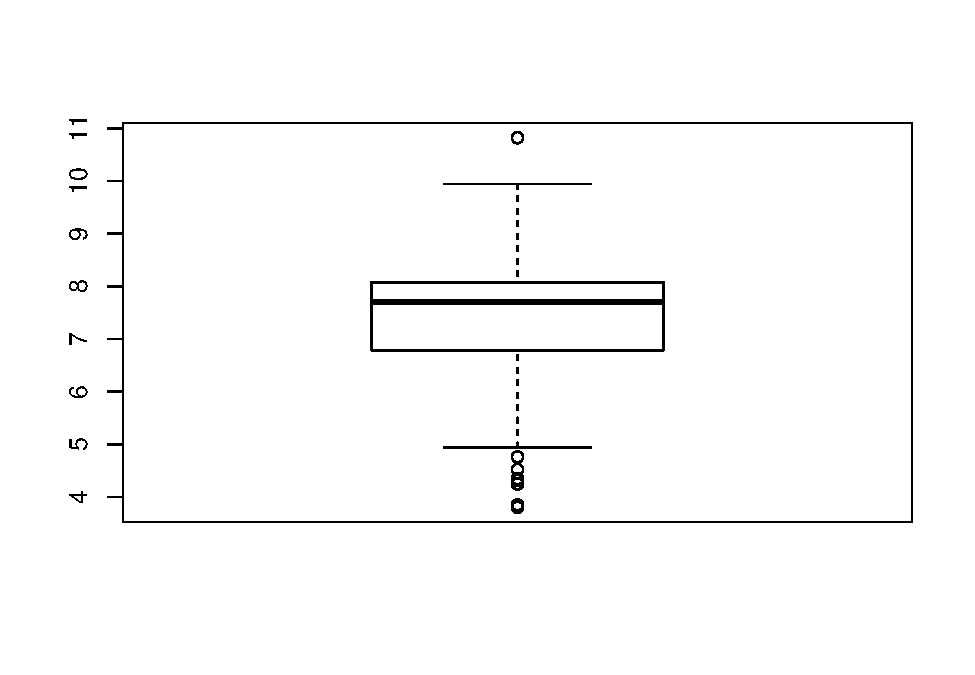
\includegraphics{RegressModelDataCamp_files/figure-latex/unnamed-chunk-26-1.pdf}

\begin{Shaded}
\begin{Highlighting}[]
\KeywordTok{quantile}\NormalTok{(logclaims, }\DataTypeTok{probs =} \FloatTok{0.75}\NormalTok{)}

\CommentTok{# BOXPLOT WITH ANNOTATION}
\KeywordTok{boxplot}\NormalTok{(logclaims, }\DataTypeTok{main =} \StringTok{"Boxplot of logclaims"}\NormalTok{)}
\KeywordTok{text}\NormalTok{(}\DecValTok{1}\NormalTok{,  }\FloatTok{7.6}\NormalTok{,  }\StringTok{"median"}\NormalTok{, }\DataTypeTok{cex =} \FloatTok{0.7}\NormalTok{)}
\KeywordTok{text}\NormalTok{(}\DecValTok{1}\NormalTok{,  }\FloatTok{6.55}\NormalTok{, }\StringTok{"25th percentile"}\NormalTok{, }\DataTypeTok{cex =} \FloatTok{0.7}\NormalTok{)}
\KeywordTok{text}\NormalTok{(}\DecValTok{1}\NormalTok{,  }\FloatTok{7.95}\NormalTok{, }\StringTok{"75th percentile"}\NormalTok{, }\DataTypeTok{cex =} \FloatTok{0.7}\NormalTok{)}
\KeywordTok{arrows}\NormalTok{(}\FloatTok{1.05}\NormalTok{, }\FloatTok{4.9}\NormalTok{, }\FloatTok{1.05}\NormalTok{, }\FloatTok{3.6}\NormalTok{, }\DataTypeTok{col =} \StringTok{"blue"}\NormalTok{, }\DataTypeTok{code =} \DecValTok{3}\NormalTok{, }\DataTypeTok{angle =} \DecValTok{20}\NormalTok{, }\DataTypeTok{length =} \FloatTok{0.1}\NormalTok{)}
\KeywordTok{text}\NormalTok{(}\FloatTok{1.1}\NormalTok{,  }\FloatTok{4.4}\NormalTok{, }\StringTok{"outliers"}\NormalTok{, }\DataTypeTok{cex =} \FloatTok{0.7}\NormalTok{)}
\KeywordTok{text}\NormalTok{(}\FloatTok{1.1}\NormalTok{, }\FloatTok{10.9}\NormalTok{, }\StringTok{"outlier"}\NormalTok{,  }\DataTypeTok{cex =} \FloatTok{0.7}\NormalTok{)}
\end{Highlighting}
\end{Shaded}

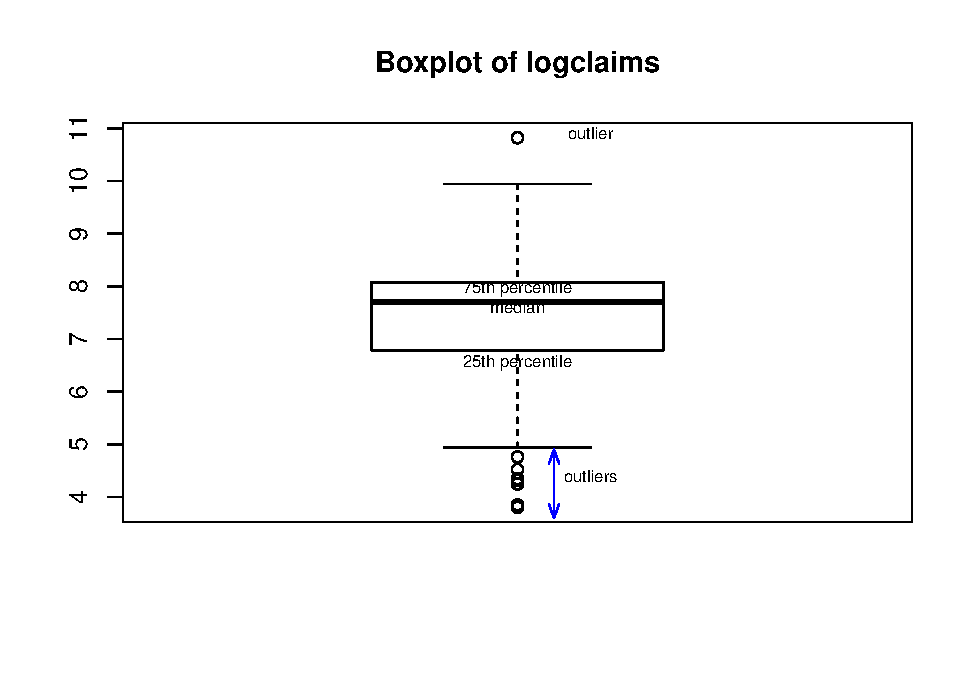
\includegraphics{RegressModelDataCamp_files/figure-latex/unnamed-chunk-26-2.pdf}

\begin{verbatim}
     75% 
8.075579 
\end{verbatim}

Show Overhead C Details. QQ Plot

\hypertarget{toggleOver1.3C}{}
\begin{Shaded}
\begin{Highlighting}[]
\KeywordTok{summary}\NormalTok{(injury)}
\KeywordTok{quantile}\NormalTok{(claims, }\DataTypeTok{probs =} \FloatTok{0.75}\NormalTok{)}
\KeywordTok{quantile}\NormalTok{(logclaims, }\DataTypeTok{probs =} \FloatTok{0.75}\NormalTok{)}
\KeywordTok{log}\NormalTok{(}\KeywordTok{quantile}\NormalTok{(claims, }\DataTypeTok{probs =} \FloatTok{0.75}\NormalTok{))}
\KeywordTok{qnorm}\NormalTok{(}\DataTypeTok{p =} \FloatTok{0.75}\NormalTok{, }\DataTypeTok{mean =} \KeywordTok{mean}\NormalTok{(logclaims), }\DataTypeTok{sd =} \KeywordTok{sd}\NormalTok{(logclaims))}
\NormalTok{(}\KeywordTok{qnorm}\NormalTok{(}\DataTypeTok{p =} \FloatTok{0.75}\NormalTok{, }\DataTypeTok{mean =} \KeywordTok{mean}\NormalTok{(logclaims), }\DataTypeTok{sd =} \KeywordTok{sd}\NormalTok{(logclaims)) }\OperatorTok{-}\KeywordTok{mean}\NormalTok{(logclaims)) }\OperatorTok{/}
\StringTok{       }\KeywordTok{sd}\NormalTok{(logclaims)}
\KeywordTok{qnorm}\NormalTok{(}\DataTypeTok{p =} \FloatTok{0.75}\NormalTok{, }\DataTypeTok{mean =} \DecValTok{0}\NormalTok{, }\DataTypeTok{sd =} \DecValTok{1}\NormalTok{)}

\CommentTok{#  QUANTILE - QUANTILE PLOT}
\KeywordTok{qqnorm}\NormalTok{(logclaims)}
\KeywordTok{qqline}\NormalTok{(logclaims)   }
\end{Highlighting}
\end{Shaded}

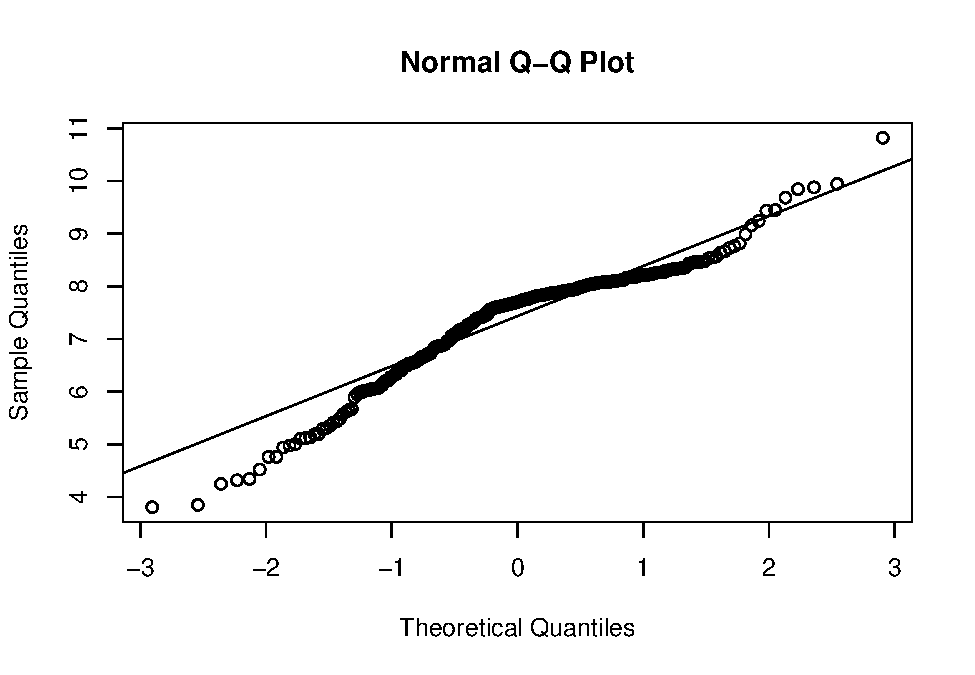
\includegraphics{RegressModelDataCamp_files/figure-latex/unnamed-chunk-27-1.pdf}

\begin{verbatim}
     claims          logclaims     
 Min.   :   45.0   Min.   : 3.807  
 1st Qu.:  892.5   1st Qu.: 6.794  
 Median : 2210.0   Median : 7.701  
 Mean   : 2697.7   Mean   : 7.388  
 3rd Qu.: 3215.0   3rd Qu.: 8.076  
 Max.   :50000.0   Max.   :10.820  
 75% 
3215 
     75% 
8.075579 
     75% 
8.075583 
[1] 8.131056
[1] 0.6744898
[1] 0.6744898
\end{verbatim}

\subsection{Exercise. Summarizing bodily injury claims with box and qq
plots}\label{exercise.-summarizing-bodily-injury-claims-with-box-and-qq-plots}

\textbf{Assignment Text}

The Massachusetts bodily injury data has already been read and used to
create the global variable \texttt{claims} representing bodily injury
claims. The previous video showed how to present the distribution of
logarithmic claims which appeared to be approximately normally
distributed. However, users are not really interested in log dollars but
want to know about a unit of measurement that is more intuitive, such as
dollars.

So this assignment is based on claims, not the logarithmic version. You
will use the functions
\href{https://www.rdocumentation.org/packages/graphics/versions/3.5.0/topics/boxplot/}{boxplot()}
and
\href{https://www.rdocumentation.org/packages/stats/versions/3.5.0/topics/qqnorm/}{qqnorm()}
to visualize the distribution through boxplots and quantile-quantile, or
qq-, plots. But, because we are working with such a skewed distribution,
do not be surprised that it is difficult to interpret these results
readily.

\textbf{Instructions}

\begin{itemize}
\tightlist
\item
  Produce a box plot for claims
\item
  Determine the 25th empirical percentile for claims using the
  \href{https://www.rdocumentation.org/packages/stats/versions/3.5.0/topics/quantile/}{quantile()}
  function.
\item
  Determine the 25th percentile for claims based on a normal
  distribution using the
  \href{https://www.rdocumentation.org/packages/stats/versions/3.5.0/topics/Normal/}{qnorm()}
  function.
\item
  Produce a normal qq plot for claims using the function
  \href{https://www.rdocumentation.org/packages/stats/versions/3.5.0/topics/qqnorm/}{qqnorm()}.
  The
  \href{https://www.rdocumentation.org/packages/stats/versions/3.5.0/topics/qqnorm/}{qqline()}
  function is handy for producing a reference line.
\end{itemize}

\textbf{Hint.} Note that
\href{https://www.rdocumentation.org/packages/stats/versions/3.5.0/topics/Normal/}{qnorm()}
(one \texttt{q}) is for a normal quantile and
\href{https://www.rdocumentation.org/packages/stats/versions/3.5.0/topics/qqnorm/}{qqnorm()}.
(two \texttt{q}'s!) is for the normal qq plot

eyJsYW5ndWFnZSI6InIiLCJwcmVfZXhlcmNpc2VfY29kZSI6IiNpbmp1cnkgPC0gcmVhZC5jc3YoXCJDU1ZEYXRhXFxcXE1hc3NCSS5jc3ZcIiwgaGVhZGVyID0gVFJVRSlcbmluanVyeSA8LSByZWFkLmNzdihcImh0dHBzOi8vYXNzZXRzLmRhdGFjYW1wLmNvbS9wcm9kdWN0aW9uL3JlcG9zaXRvcmllcy8yNjEwL2RhdGFzZXRzLzhjY2ExOWQwNTAzZmNmNmU5ZDMwZDljYjkxMmRlNWJhOTVlY2I5YzEvTWFzc0JJLmNzdlwiLCBoZWFkZXIgPSBUUlVFKVxuY2xhaW1zIDwtIGluanVyeSRjbGFpbXMiLCJzYW1wbGUiOiIjUHJvZHVjZSBhIGJveCBwbG90IGZvciBjbGFpbXNcbl9fXyhjbGFpbXMpXG5cbiNEZXRlcm1pbmUgdGhlIDI1dGggZW1waXJpY2FsIHBlcmNlbnRpbGUgZm9yIGNsYWltc1xucTI1IDwtIF9fXyhjbGFpbXMsIHByb2JzID0gX19fKVxucTI1XG5cbiNEZXRlcm1pbmUgdGhlIDI1dGggcGVyY2VudGlsZSBmb3IgY2xhaW1zIGJhc2VkIG9uIGEgbm9ybWFsIGRpc3RyaWJ1dGlvblxucW4yNSA8LSBfX18ocCA9IF9fXywgbWVhbiA9IG1lYW4oY2xhaW1zKSwgc2QgPSBzZChjbGFpbXMpKVxucW4yNVxuXG4jUHJvZHVjZSBhIG5vcm1hbCBxcSBwbG90IGZvciBjbGFpbXNcbl9fXyhjbGFpbXMpXG5fX18oY2xhaW1zKSIsInNvbHV0aW9uIjoiIyBTb2x1dGlvblxuYm94cGxvdChjbGFpbXMpXG5xMjUgPC0gcXVhbnRpbGUoY2xhaW1zLCBwcm9icyA9IDAuMjUpXG5xMjVcbnFuMjUgPC0gcW5vcm0ocCA9IDAuMjUsIG1lYW4gPSBtZWFuKGNsYWltcyksIHNkID0gc2QoY2xhaW1zKSlcbnFuMjVcbnFxbm9ybShjbGFpbXMpXG5xcWxpbmUoY2xhaW1zKSAgICIsInNjdCI6ImV4KCkgJT4lIGNoZWNrX2Z1bmN0aW9uKFwiYm94cGxvdFwiKSAlPiUgY2hlY2tfYXJnKFwieFwiKSAlPiUgY2hlY2tfZXF1YWwoaW5jb3JyZWN0X21zZz1cIlBsZWFzZSBjcmVhdGUgYSBib3hwbG90IG9mIGBjbGFpbXNgLlwiKVxuZXgoKSAlPiUgY2hlY2tfZnVuY3Rpb24oXCJxdWFudGlsZVwiKSAlPiUgY2hlY2tfYXJnKFwicHJvYnNcIikgJT4lIGNoZWNrX2VxdWFsKGluY29ycmVjdF9tc2c9XCJJZiB3ZSB3YW50IHRvIGZpbmQgdGhlIFl0aCBwZXJjZW50aWxlLCBtYWtlIHN1cmUgdG8gc2V0IHByb2JzIGVxdWFsIHRvIFkgaW4gZGVjaW1hbCBmb3JtYXQuXCIpXG5leCgpICU+JSBjaGVja19vYmplY3QoXCJxMjVcIix1bmRlZmluZWRfbXNnPVwiTWFrZSBzdXJlIHRvIGFzc2lnbiB0aGUgMjV0aCBxdWFudGlsZSB0byBgcTI1XCIpICU+JSBjaGVja19lcXVhbCgpXG5leCgpICU+JSBjaGVja19vYmplY3QoXCJxbjI1XCIsdW5kZWZpbmVkX21zZz1cIk1ha2Ugc3VyZSB0byBhc3NpZ24gdGhlIG5vcm1hbCB2YWx1ZSBhc3NvY2lhdGVkIHdpdGggdGhlIDI1dGggcGVyY2VudGlsZSB0byBxbjI1XCIpICU+JSBjaGVja19lcXVhbCgpXG5leCgpICU+JSBjaGVja19mdW5jdGlvbihcInFxbm9ybVwiKSAlPiUgY2hlY2tfYXJnKFwieVwiKSAlPiUgY2hlY2tfZXF1YWwoaW5jb3JyZWN0X21zZz1cIk1ha2Ugc3VyZSB0aGF0IHlvdSBhcmUgY3JlYXRpbmcgYSBxcS1wbG90IGZvciBgY2xhaW1zYC5cIilcbmV4KCkgJT4lIGNoZWNrX2Z1bmN0aW9uKFwicXFsaW5lXCIpICU+JSBjaGVja19hcmcoXCJ5XCIpICU+JSBjaGVja19lcXVhbChpbmNvcnJlY3RfbXNnPVwiTWFrZSBzdXJlIHRoYXQgeW91IGFyZSBhZGRpbmcgYSBxcS1saW5lIGZvciBgY2xhaW1zYC5cIilcbnN1Y2Nlc3NfbXNnKFwiQ29uZ3JhdHVsYXRpb25zIG9uIGxlYXJuaW5nIGFib3V0IGJveCBhbmQgcXEgcGxvdHMuIEFsdGhvdWdoIHlvdSBhcmUgdW5saWtlbHkgdG8gc2hvdyB0aGVzZSBwbG90cyB0byBjb25zdW1lcnMgb2YgeW91ciBhbmFseXNpcywgeW91IHdpbGwgZmluZCB0aGVtIHVzZWZ1bCB0b29scyBhcyB3ZSBleHBsb3JlIG11bHRpdmFyaWF0ZSBhc3BlY3RzIG9mIGRhdGEuXCIpIn0=

\subsection{Exercise. Effects on distributions of removing the largest
claim}\label{exercise.-effects-on-distributions-of-removing-the-largest-claim}

\textbf{Assignment Text}

The Massachusetts bodily injury dataframe \texttt{injury} has been read
in; our focus is on the \texttt{claims} variable in that dataset.

In the previous exercise, we learned that the Massachusetts bodily
injury \texttt{claims} distribution was not even close to approximately
normal (as evidenced by the box and qq- plots). Non-normality may be
induced by skewness (that we will handle via transformations in the next
section). But, seeming non-normality can also be induced by one or two
very large observations (called an \emph{outlier} later in the course).
So, this exercise examines the effects on the distribution of removing
the largest claims.

\textbf{Instructions}

\begin{itemize}
\tightlist
\item
  Use the function
  \href{https://www.rdocumentation.org/packages/utils/versions/3.5.0/topics/head}{tail()}
  to examine the \texttt{injury} dataset and identify the largest claim
\item
  Use the function
  \href{https://www.rdocumentation.org/packages/base/versions/3.5.0/topics/subset}{subset()}
  to create a subset omitting the largest claim
\item
  Compare the summary statistics of the omitted claim distribution to
  the full distribution
\item
  Compare the two distributions visually via histograms plotted next to
  another. \texttt{par(mfrow\ =\ c(1,\ 2))} is used to organize the
  plots you create. Do not alter this code.
\end{itemize}

\textbf{Hint.} For this data set, the {[}subset(){]} argument
\texttt{claims\ \textless{}\ 25000} will keep all but the largest claim

eyJsYW5ndWFnZSI6InIiLCJwcmVfZXhlcmNpc2VfY29kZSI6IiNpbmp1cnkgPC0gcmVhZC5jc3YoXCJDU1ZEYXRhXFxcXE1hc3NCSS5jc3ZcIiwgaGVhZGVyID0gVFJVRSlcbmluanVyeSA8LSByZWFkLmNzdihcImh0dHBzOi8vYXNzZXRzLmRhdGFjYW1wLmNvbS9wcm9kdWN0aW9uL3JlcG9zaXRvcmllcy8yNjEwL2RhdGFzZXRzLzhjY2ExOWQwNTAzZmNmNmU5ZDMwZDljYjkxMmRlNWJhOTVlY2I5YzEvTWFzc0JJLmNzdlwiLCBoZWFkZXIgPSBUUlVFKVxuY2xhaW1zIDwtIGluanVyeSRjbGFpbXMiLCJzYW1wbGUiOiIjIEV4YW1pbmUgdGhlIHRhaWwgb2YgdGhlIGBpbmp1cnlgIGRhdGFzZXRcbnRhaWwoX19fKVxuXG4jIENyZWF0ZSBhIHN1YnNldCBvbWl0dGluZyB0aGUgbGFyZ2VzdCBjbGFpbVxuaW5qdXJ5MiA8LSBzdWJzZXQoaW5qdXJ5LCBfX18pXG5cbiMgQ29tcGFyZSB0aGUgc3VtbWFyeSBzdGF0aXN0aWNzIG9mIHRoZSBvbWl0dGVkIGNsYWltIGRpc3RyaWJ1dGlvbiB0byB0aGUgZnVsbCBkaXN0cmlidXRpb25cbnN1bW1hcnkoX19fKVxuc3VtbWFyeShpbmp1cnkyKVxuXG4jIENvbXBhcmUgdGhlIHR3byBkaXN0cmlidXRpb25zIHZpc3VhbGx5IHZpYSBoaXN0b2dyYW1zIHBsb3R0ZWQgbmV4dCB0byBhbm90aGVyXG5wYXIobWZyb3cgPSBjKDEsIDIpKVxuaGlzdChfX18sIGZyZXEgPSBGQUxTRSwgIG1haW4gPSBcIkZ1bGwgRGF0YVwiKVxuaGlzdChfX18sIGZyZXEgPSBGQUxTRSwgIG1haW4gPSBcIkxhcmdlc3QgQ2xhaW0gT21pdHRlZFwiKSIsInNvbHV0aW9uIjoidGFpbChpbmp1cnkpXG5pbmp1cnkyIDwtIHN1YnNldChpbmp1cnksIGNsYWltcyA8IDI1MDAwIClcbnN1bW1hcnkoaW5qdXJ5KVxuc3VtbWFyeShpbmp1cnkyKVxucGFyKG1mcm93ID0gYygxLCAyKSlcbmhpc3QoY2xhaW1zLCBmcmVxID0gRkFMU0UsICBtYWluID0gXCJGdWxsIERhdGFcIilcbmhpc3QoaW5qdXJ5MiRjbGFpbXMsIGZyZXEgPSBGQUxTRSwgIG1haW4gPSBcIkxhcmdlc3QgQ2xhaW0gT21pdHRlZFwiKSIsInNjdCI6ImV4KCkgJT4lIGNoZWNrX2Z1bmN0aW9uKFwidGFpbFwiKSAlPiUgY2hlY2tfYXJnKFwieFwiKSAlPiUgY2hlY2tfZXF1YWwoaW5jb3JyZWN0X21zZz1cIk1ha2Ugc3VyZSB0byB1c2UgdGFpbCB0byBzZWUgdGhlIGxhcyA2IGVudHJpZXMgaW4gYGluanVyeWAuXCIpXG5leCgpICU+JSBjaGVja19vYmplY3QoXCJpbmp1cnkyXCIpICU+JSBjaGVja19lcXVhbChpbmNvcnJlY3RfbXNnPVwiTWFrZSBzdXJlIHRoYXQgYGluanVyeTJgIGlzIHRoZSBzYW1lIGFzIGBpbmp1cnlgIGJ1dCB3aXRob3V0IHRoZSBsYXJnZXN0IGNsYWltLiBUcnkgYW5kIHRoaW5rIG9mIGNyZWF0aXZlIHdheXMgdG8gcmVtb3ZlIHRoYXQgb2JzZXJ2YXRpb24gZnJvbSB0aGUgZGF0YSFcIilcbmV4KCkgJT4lIGNoZWNrX2Z1bmN0aW9uKFwic3Vic2V0XCIpXG5leCgpICU+JSBjaGVja19mdW5jdGlvbihcInN1bW1hcnlcIixpbmRleD0xKSAlPiUgY2hlY2tfYXJnKFwib2JqZWN0XCIpICU+JSBjaGVja19lcXVhbChpbmNvcnJlY3RfbXNnPVwiTWFrZSBzdXJlIHRvIGdldCBzdW1tYXJ5IHN0YXRpc3RpY3Mgb2YgYGluanVyeTJgLlwiKVxuZXgoKSAlPiUgY2hlY19mdW5jdGlvbihcInN1bW1hcnlcIixpbmRleD0yKSAlPiUgY2hlY2tfYXJnKFwib2JqZWN0XCIpICU+JSBjaGVja19lcXVhbCgpXG5leCgpICU+JSBjaGVja19mdW5jdGlvbihcInBhclwiKSAlPiUgY2hlY2tfYXJnKFwibWZyb3dcIikgJT4lIGNoZWNrX2VxdWFsKGluY29ycmVjdF9tc2c9XCJQbGVhc2UgZG9udCBjaGFuZ2UgdGhpcyBwYXJ0LiBpdCBzaG91bGQgcmVhZCBgcGFyKG1mcm93PWMoMiwxKSlgXCIpXG5leCgpICU+JSBjaGVja19mdW5jdGlvbihcImhpc3RcIixpbmRleD0xKSAlPiUge1xuICBjaGVja19hcmcoXCJ4XCIpICU+JSBjaGVja19lcXVhbChpbmNvcnJlY3RfbXNnPVwiQ3JlYXRlIHRoZSBmaXJzdCBoaXN0b2dyYW0gdXNpbmcgYWxsIG9mIHRoZSBvYnNlcnZlZCBjbGFpbXMuXCIpXG4gIGNoZWNrX2FyZyhcImZyZXFcIikgJT4lIGNoZWNrX2VxdWFsKGluY29ycmVjdF9tc2c9XCJNYWtlIHN1cmUgdG8gY3JlYXRlIGEgZGVuc2l0eSBoaXN0b2dyYW0gaW5zdGVhZCBvZiBhIGZyZXF1ZW5jeSBoaXN0b2dyYW0uXCIpXG59XG5leCgpICU+JSBjaGVja19mdW5jdGlvbihcImhpc3RcIixpbmRleD0yKSAlPiUge1xuICBjaGVja19hcmcoXCJ4XCIpICU+JSBjaGVja19lcXVhbChpbmNvcnJlY3RfbXNnPVwiTWFrZSBzdXJlIHRvIGNyZWF0ZSB0aGUgc2Vjb25kIGhpc3RvZ3JhbSBiYXNlZCBvbiBjbGFpbXMgd2l0aCB0aGUgbGFyZ2VzdCBvbmUgcmVtb3ZlZC5cIilcbiAgY2hlY2tfYXJnKFwiZnJlcVwiKSAlPiUgY2hlY2tfZXF1YWwoaW5jb3JyZWN0X21zZz1cIk1ha2Ugc3VyZSB0byBjcmVhdGUgYSBkZW5zaXR5IGhpc3RvZ3JhbSBpbnN0ZWFkIG9mIGEgZnJlcXVlbmN5IGhpc3RvZ3JhbS5cIilcbn1cbnN1Y2Nlc3NfbXNnKFwiQ29uZ3JhdHVsYXRpb25zISBUaGUgZ29hbCBvZiBwcmVkaWN0aXZlIG1vZGVsaW5nIGlzIHRvIGRpc2NvdmVyIHBhdHRlcm5zIGluIHRoZSBkYXRhLiBIb3dldmVyLCBzb21ldGltZXMgc2VlbWluZyAncGF0dGVybnMnIGFyZSB0aGUgcmVzdWx0IG9mIG9uZSBvciB0d28gdW51c3VhbCBvYnNlcnZhdGlvbnMuIFVudXN1YWwgb2JzZXJ2YXRpb25zIG1heSBiZSBkdWUgdG8gaW5jb3JyZWN0IGRhdGEgZ2F0aGVyaW5nIHByb2NlZHVyZXMgb3IganVzdCBkdWUgdG8gd2lsZCBmbHVjdHVhdGlvbnMgaW4gYSBwcm9jZXNzIG9mIGludGVyZXN0IGJ1dCBhcmUgY29tbW9uIGluIHByZWRpY3RpdmUgbW9kZWxpbmcuXCIpIn0=

\section{Transformations}\label{transformations}

\begin{center}\rule{0.5\linewidth}{\linethickness}\end{center}

In this exercise, you learn how to:

\begin{itemize}
\tightlist
\item
  Symmetrize a skewed distribution using a logarithmic transformation
\end{itemize}

\begin{center}\rule{0.5\linewidth}{\linethickness}\end{center}

\subsection{Video}\label{video-3}

\subsubsection*{Video Overhead Details}\label{video-overhead-details-3}
\addcontentsline{toc}{subsubsection}{Video Overhead Details}

Show Overhead A Details. Simulate a moderately skewed distribution, with
transforms

\hypertarget{toggleOver1.4A}{}
\begin{Shaded}
\begin{Highlighting}[]
\CommentTok{#  FIGURE 1.7 - SIMULATE CHI-SQUARE, CREATE 3 TRANSFORMATIONS}
\KeywordTok{set.seed}\NormalTok{(}\DecValTok{1237}\NormalTok{)                  }\CommentTok{# set the seed of the random number generator}
                                \CommentTok{# allows us to replicate results}
\NormalTok{X1 <-}\StringTok{ }\DecValTok{10000}\OperatorTok{*}\KeywordTok{rchisq}\NormalTok{(}\DecValTok{500}\NormalTok{, }\DataTypeTok{df =} \DecValTok{2}\NormalTok{) }\CommentTok{# generate variables randomly from a skewed distribution}
\NormalTok{X2 <-}\StringTok{ }\NormalTok{X1}\OperatorTok{^}\NormalTok{(}\FloatTok{0.5}\NormalTok{)                  }\CommentTok{# square root transform, could also use sqrt(X1)}
\NormalTok{X3 <-}\StringTok{ }\KeywordTok{log}\NormalTok{(X1)                   }\CommentTok{# logarithmic transform}
\NormalTok{X4 <-}\StringTok{ }\OperatorTok{-}\DecValTok{1}\OperatorTok{/}\NormalTok{X1                     }\CommentTok{# negative reciprocal transform}
\end{Highlighting}
\end{Shaded}

Show Overhead B Details. Visualize the distributions

\hypertarget{toggleOver1.4B}{}
\begin{Shaded}
\begin{Highlighting}[]
\KeywordTok{par}\NormalTok{(}\DataTypeTok{mfrow =} \KeywordTok{c}\NormalTok{(}\DecValTok{2}\NormalTok{, }\DecValTok{2}\NormalTok{), }\DataTypeTok{cex =}\NormalTok{ .}\DecValTok{75}\NormalTok{, }\DataTypeTok{mar =} \KeywordTok{c}\NormalTok{(}\DecValTok{3}\NormalTok{,}\DecValTok{5}\NormalTok{,}\FloatTok{1.5}\NormalTok{,}\DecValTok{0}\NormalTok{))}
\KeywordTok{hist}\NormalTok{(X1, }\DataTypeTok{freq =} \OtherTok{FALSE}\NormalTok{,  }\DataTypeTok{nclass =} \DecValTok{16}\NormalTok{, }\DataTypeTok{main =} \StringTok{""}\NormalTok{, }\DataTypeTok{xlab =} \StringTok{""}\NormalTok{, }\DataTypeTok{ylab =} \StringTok{""}\NormalTok{, }
      \DataTypeTok{las =} \DecValTok{1}\NormalTok{, }\DataTypeTok{yaxt =} \StringTok{"n"}\NormalTok{,}\DataTypeTok{xlim =} \KeywordTok{c}\NormalTok{(}\DecValTok{0}\NormalTok{,}\DecValTok{200000}\NormalTok{),}\DataTypeTok{ylim =} \KeywordTok{c}\NormalTok{(}\DecValTok{0}\NormalTok{,.}\DecValTok{00005}\NormalTok{))}
\KeywordTok{axis}\NormalTok{(}\DecValTok{2}\NormalTok{, }\DataTypeTok{at =} \KeywordTok{seq}\NormalTok{(}\DecValTok{0}\NormalTok{,.}\DecValTok{00005}\NormalTok{,.}\DecValTok{00001}\NormalTok{),}\DataTypeTok{las =} \DecValTok{1}\NormalTok{, }\DataTypeTok{cex =}\NormalTok{ .}\DecValTok{3}\NormalTok{, }
  \DataTypeTok{labels =} \KeywordTok{c}\NormalTok{(}\StringTok{"0"}\NormalTok{, }\StringTok{"0.00001"}\NormalTok{, }\StringTok{"0.00002"}\NormalTok{,}\StringTok{"0.00003"}\NormalTok{, }\StringTok{"0.00004"}\NormalTok{, }\StringTok{"0.00005"}\NormalTok{))}
\KeywordTok{mtext}\NormalTok{(}\StringTok{"Density"}\NormalTok{, }\DataTypeTok{side =} \DecValTok{2}\NormalTok{, }\DataTypeTok{at =}\NormalTok{ .}\DecValTok{000055}\NormalTok{, }\DataTypeTok{las =} \DecValTok{1}\NormalTok{, }\DataTypeTok{cex =}\NormalTok{ .}\DecValTok{75}\NormalTok{)}
\KeywordTok{mtext}\NormalTok{(}\StringTok{"y"}\NormalTok{, }\DataTypeTok{side =} \DecValTok{1}\NormalTok{, }\DataTypeTok{cex =}\NormalTok{ .}\DecValTok{75}\NormalTok{, }\DataTypeTok{line =} \DecValTok{2}\NormalTok{)}

\KeywordTok{par}\NormalTok{(}\DataTypeTok{mar =} \KeywordTok{c}\NormalTok{(}\DecValTok{3}\NormalTok{,}\DecValTok{4}\NormalTok{,}\FloatTok{1.5}\NormalTok{,}\FloatTok{0.2}\NormalTok{))}
\KeywordTok{hist}\NormalTok{(X2, }\DataTypeTok{freq =} \OtherTok{FALSE}\NormalTok{,  }\DataTypeTok{nclass =} \DecValTok{16}\NormalTok{, }\DataTypeTok{main =} \StringTok{""}\NormalTok{, }\DataTypeTok{xlab =} \StringTok{""}\NormalTok{, }\DataTypeTok{ylab =} \StringTok{""}\NormalTok{, }
      \DataTypeTok{las =} \DecValTok{1}\NormalTok{,}\DataTypeTok{xlim =} \KeywordTok{c}\NormalTok{(}\DecValTok{0}\NormalTok{,}\DecValTok{400}\NormalTok{), }\DataTypeTok{ylim =} \KeywordTok{c}\NormalTok{(}\DecValTok{0}\NormalTok{,.}\DecValTok{008}\NormalTok{))}
\KeywordTok{mtext}\NormalTok{(}\StringTok{"Density"}\NormalTok{, }\DataTypeTok{side =} \DecValTok{2}\NormalTok{, }\DataTypeTok{at =}\NormalTok{ .}\DecValTok{0088}\NormalTok{, }\DataTypeTok{las =} \DecValTok{1}\NormalTok{, }\DataTypeTok{cex =}\NormalTok{ .}\DecValTok{75}\NormalTok{)}
\KeywordTok{mtext}\NormalTok{(}\StringTok{"Square root of y"}\NormalTok{, }\DataTypeTok{side =} \DecValTok{1}\NormalTok{, }\DataTypeTok{cex =}\NormalTok{ .}\DecValTok{75}\NormalTok{, }\DataTypeTok{line =} \DecValTok{2}\NormalTok{)}

\KeywordTok{par}\NormalTok{(}\DataTypeTok{mar =} \KeywordTok{c}\NormalTok{(}\FloatTok{3.2}\NormalTok{,}\DecValTok{5}\NormalTok{,}\DecValTok{1}\NormalTok{,}\DecValTok{0}\NormalTok{))}
\KeywordTok{hist}\NormalTok{(X3,  }\DataTypeTok{freq =} \OtherTok{FALSE}\NormalTok{,  }\DataTypeTok{nclass =} \DecValTok{16}\NormalTok{, }\DataTypeTok{main =} \StringTok{""}\NormalTok{, }\DataTypeTok{xlab =} \StringTok{""}\NormalTok{, }\DataTypeTok{ylab =} \StringTok{""}\NormalTok{, }\DataTypeTok{las =} \DecValTok{1}\NormalTok{, }\DataTypeTok{ylim =} \KeywordTok{c}\NormalTok{(}\DecValTok{0}\NormalTok{,.}\DecValTok{4}\NormalTok{))}
\KeywordTok{mtext}\NormalTok{(}\StringTok{"Density"}\NormalTok{, }\DataTypeTok{side =} \DecValTok{2}\NormalTok{, }\DataTypeTok{at =}\NormalTok{ .}\DecValTok{44}\NormalTok{, }\DataTypeTok{las =} \DecValTok{1}\NormalTok{, }\DataTypeTok{cex =}\NormalTok{ .}\DecValTok{75}\NormalTok{)}
\KeywordTok{mtext}\NormalTok{(}\StringTok{"Logarithmic y"}\NormalTok{, }\DataTypeTok{side =} \DecValTok{1}\NormalTok{, }\DataTypeTok{cex =}\NormalTok{ .}\DecValTok{75}\NormalTok{, }\DataTypeTok{line =} \DecValTok{2}\NormalTok{)}

\KeywordTok{par}\NormalTok{(}\DataTypeTok{mar =} \KeywordTok{c}\NormalTok{(}\FloatTok{3.2}\NormalTok{,}\DecValTok{4}\NormalTok{,}\DecValTok{1}\NormalTok{,}\FloatTok{0.2}\NormalTok{))}
\KeywordTok{hist}\NormalTok{(X4, }\DataTypeTok{freq =} \OtherTok{FALSE}\NormalTok{,  }\DataTypeTok{nclass =} \DecValTok{16}\NormalTok{, }\DataTypeTok{main =} \StringTok{""}\NormalTok{,}\DataTypeTok{xlab =} \StringTok{""}\NormalTok{, }\DataTypeTok{ylab =} \StringTok{""}\NormalTok{, }\DataTypeTok{las =} \DecValTok{1}\NormalTok{, }\DataTypeTok{ylim =} \KeywordTok{c}\NormalTok{(}\DecValTok{0}\NormalTok{,}\DecValTok{100}\NormalTok{))}
\KeywordTok{mtext}\NormalTok{(}\StringTok{"Density"}\NormalTok{, }\DataTypeTok{side =} \DecValTok{2}\NormalTok{, }\DataTypeTok{at =} \DecValTok{110}\NormalTok{, }\DataTypeTok{las =} \DecValTok{1}\NormalTok{, }\DataTypeTok{cex =}\NormalTok{ .}\DecValTok{75}\NormalTok{)}
\KeywordTok{mtext}\NormalTok{(}\StringTok{"Negative reciprocal of y"}\NormalTok{, }\DataTypeTok{side =} \DecValTok{1}\NormalTok{, }\DataTypeTok{cex =}\NormalTok{ .}\DecValTok{75}\NormalTok{, }\DataTypeTok{line =} \DecValTok{2}\NormalTok{)}
\end{Highlighting}
\end{Shaded}

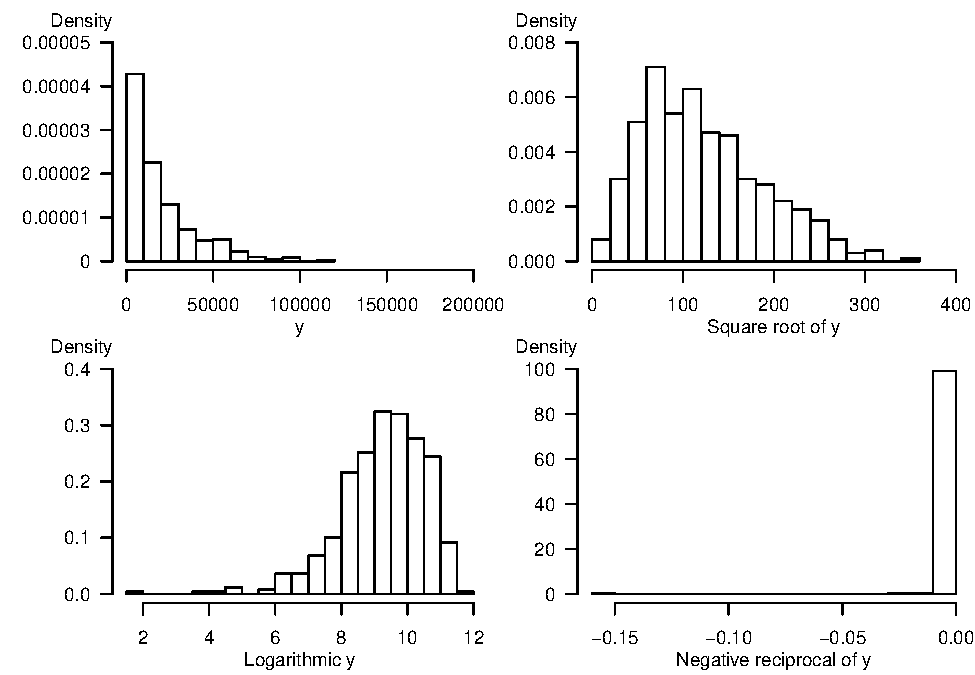
\includegraphics{RegressModelDataCamp_files/figure-latex/unnamed-chunk-37-1.pdf}

\subsection{Exercise. Distribution of transformed bodily injury
claims}\label{exercise.-distribution-of-transformed-bodily-injury-claims}

\textbf{Assignment Text}

We have now examined the distributions of bodily injury claims and its
logarithmic version. Grudgingly, we have concluded that to fit a normal
curve the logarithmic version of claims is a better choice (again, we
really do not like log dollars but you'll get used to it in this
course). But, why logarithmic and not some other transformations?

A partial response to this question will appear in later chapters when
we describe interpretation of regression coefficients. Another partial
response is that the log transform seems to work well with skewed
insurance data sets, as we demonstrate visually in this exercise.

\textbf{Instructions}

Use the code \texttt{par(mfrow\ =\ c(2,\ 2))} so that four graphs appear
in a 2 by 2 matrix format for easy comparisons. Plot the
\href{https://www.rdocumentation.org/packages/stats/versions/3.5.1/topics/density}{density()}
of

\begin{itemize}
\tightlist
\item
  claims
\item
  square root of claims
\item
  logarithmic claims
\item
  negative reciprocal of claims
\end{itemize}

\textbf{Hint.} For negative reciprocal claims, use
\texttt{plot(density(-claims\^{}(-1)))}

eyJsYW5ndWFnZSI6InIiLCJwcmVfZXhlcmNpc2VfY29kZSI6IiNpbmp1cnkgPC0gcmVhZC5jc3YoXCJDU1ZEYXRhXFxcXE1hc3NCSS5jc3ZcIiwgaGVhZGVyID0gVFJVRSlcbmluanVyeSA8LSByZWFkLmNzdihcImh0dHBzOi8vYXNzZXRzLmRhdGFjYW1wLmNvbS9wcm9kdWN0aW9uL3JlcG9zaXRvcmllcy8yNjEwL2RhdGFzZXRzLzhjY2ExOWQwNTAzZmNmNmU5ZDMwZDljYjkxMmRlNWJhOTVlY2I5YzEvTWFzc0JJLmNzdlwiLCBoZWFkZXIgPSBUUlVFKVxuY2xhaW1zIDwtIGluanVyeSRjbGFpbXMiLCJzYW1wbGUiOiIjVGhpcyBjb2RlIGhlbHBzIHRvIG9yZ2FuaXplIHRoZSBmb3VyIGdyYXBocyBpbnRvIGEgMiBieSAyIGZvcm1hdFxucGFyKG1mcm93ID0gYygyLCAyKSlcbiNQbG90IHRoZSBkZW5zaXR5IG9mIGNsYWltc1xucGxvdChkZW5zaXR5KF9fXykpXG5cbiNQbG90IHRoZSBkZW5zaXR5IG9mIHNxdWFyZSByb290IG9mIGNsYWltc1xucGxvdChkZW5zaXR5KF9fXykpIFxuXG4jUGxvdCB0aGUgZGVuc2l0eSBvZiBsb2dhcml0aG1pYyBjbGFpbXNcbnBsb3QoZGVuc2l0eShfX18pKVxuXG4jUGxvdCB0aGUgZGVuc2l0eSBvZiB0aGUgbmVnYXRpdmUgcmVjaXByb2NhbCBvZiBjbGFpbXNcbnBsb3QoZGVuc2l0eShfX18pKSIsInNvbHV0aW9uIjoicGFyKG1mcm93ID0gYygyLCAyKSlcbnBsb3QoZGVuc2l0eShjbGFpbXMpKSAgICBcbnBsb3QoZGVuc2l0eShjbGFpbXNeKDAuNSkpKSAgXG5wbG90KGRlbnNpdHkobG9nKGNsYWltcykpKSAgXG5wbG90KGRlbnNpdHkoLWNsYWltc14oLTEpKSkgICIsInNjdCI6ImV4KCkgJT4lIGNoZWNrX2Z1bmN0aW9uKFwicGFyXCIpICU+JSBjaGVja19hcmcoXCJtZnJvd1wiKSAlPiUgY2hlY2tfZXF1YWwoXCJQbGVhc2UgZG8gbm90IGNoYW5nZSB0aGlzIHBhcnQgb2YgdGhlIGNvZGUuIEl0IHNob3VsZCByZWFkIGBwYXIobWZyb3c9YygyLDIpKWBcIilcbmV4KCkgJT4lIGNoZWNrX2Z1bmN0aW9uKFwicGxvdFwiLGluZGV4PTEsbm90X2NhbGxlZF9tc2c9XCJEaWQgeW91IHBsb3QgdGhlIGRlbnNpdHkgb2YgY2xhaW1zP1wiKSAlPiUgY2hlY2tfYXJnKFwieFwiKSAlPiUgY2hlY2tfZXF1YWwoaW5jb3JyZWN0X21zZz1cIk1ha2Ugc3VyZSB0byBjcmVhdGUgdGhlIGZpcnN0IGhpc3RvZ3JhbSB1c2luZyBgY2xhaW1zYFwiKVxuZXgoKSAlPiUgY2hlY2tfb3IoXG5jaGVja19mdW5jdGlvbiguLFwicGxvdFwiKSAlPiUgY2hlY2tfYXJnKC4sIFwieFwiKSAlPiUgY2hlY2tfZXF1YWwoKSxcbiAgb3ZlcnJpZGVfc29sdXRpb24oLixcInBsb3QoZGVuc2l0eShzcXJ0KGNsYWltcykpKVwiKSAlPiUgY2hlY2tfZnVuY3Rpb24oXCJwbG90XCIpICU+JSBjaGVja19hcmcoLiwgXCJ4XCIpICU+JSBjaGVja19lcXVhbCgpXG4pXG5leCgpICU+JSBjaGVja19mdW5jdGlvbihcInBsb3RcIixpbmRleD0zLG5vdF9jYWxsZWRfbXNnPVwiRGlkIHlvdSBwbG90IHRoZSBkZW5zaXR5IG9mIGxvZ2FyaXRobWljIGNsYWltcz9cIikgJT4lIGNoZWNrX2FyZyhcInhcIikgJT4lIGNoZWNrX2VxdWFsKGluY29ycmVjdF9tc2c9XCJNYWtlIHN1cmUgdG8gY3JlYXRlIHRoZSB0aGlyZCBoaXN0b2dyYW0gYmFzZWQgb24gdGhlIG5hdHVyYWwgbG9nIG9mIGBjbGFpbXNgLlwiKVxuZXgoKSAlPiUgY2hlY2tfZnVuY3Rpb24oXCJwbG90XCIsaW5kZXg9NCxub3RfY2FsbGVkX21zZz1cIkRpZCB5b3UgcGxvdCB0aGUgZGVuc2l0eSBvZiB0aGUgbmVnYXRpdmUgcmVjaXByb2NhbCBvZiBjbGFpbXM/XCIpICU+JSBjaGVja19hcmcoXCJ4XCIpICU+JSBjaGVja19lcXVhbChpbmNvcnJlY3RfbXNnPVwiTWFrZSBzdXJlIHRvIGNyZWF0ZSB0aGUgZm91cnRoIGhpc3RvZ3JhbSBiYXNlZCBvbiB0aGUgbmVnYXRpdmUgcmVjaXByb2NhbCAoKSBvZiBgY2xhaW1zYC5cIilcbnN1Y2Nlc3NfbXNnKFwiRXhjZWxsZW50ISBUcmFuc2Zvcm1hdGlvbnMgb2YgZGF0YSBpcyBhIHRvb2wgdGhhdCBpbmNyZWRpYmx5IGV4cGFuZHMgcG90ZW50aWFsIGFwcGxpY2FiaWxpdHkgb2YgKGxpbmVhcikgcmVncmVzc2lvbiB0ZWNobmlxdWVzLlwiKSJ9

\chapter{Basic Linear Regression}\label{basic-linear-regression}

\textbf{Chapter description}

This chapter considers regression in the case of only one explanatory
variable. Despite this seeming simplicity, many deep ideas of regression
can be developed in this framework. By limiting ourselves to the one
variable case, we can illustrate the relationships between two variables
graphically. Graphical tools prove to be important for developing a link
between the data and a predictive model.

\section{Correlation}\label{correlation}

\begin{center}\rule{0.5\linewidth}{\linethickness}\end{center}

In this section, you learn how to:

\begin{itemize}
\tightlist
\item
  Calculate and interpret a correlation coefficient
\item
  Interpret correlation coefficients by visualizing scatter plots
\end{itemize}

\begin{center}\rule{0.5\linewidth}{\linethickness}\end{center}

\subsection{Video}\label{video-4}

\subsubsection*{Video Overhead Details}\label{video-overhead-details-4}
\addcontentsline{toc}{subsubsection}{Video Overhead Details}

Show Overhead A Details. Wisconsin lottery data description

\hypertarget{toggleOver2.1A}{}
\begin{Shaded}
\begin{Highlighting}[]
\NormalTok{Lot <-}\StringTok{ }\KeywordTok{read.csv}\NormalTok{(}\StringTok{"CSVData}\CharTok{\textbackslash{}\textbackslash{}}\StringTok{Wisc_lottery.csv"}\NormalTok{)}
\CommentTok{#Lot <- read.csv("https://assets.datacamp.com/production/repositories/2610/datasets/a792b30fb32b0896dd6894501cbab32b5d48df51/Wisc_lottery.csv", header = TRUE)}
\KeywordTok{str}\NormalTok{(Lot)}
\end{Highlighting}
\end{Shaded}

\begin{verbatim}
'data.frame':   50 obs. of  3 variables:
 $ pop    : int  435 4823 2469 2051 13337 17004 38283 9859 4464 20958 ...
 $ sales  : num  1285 3571 2407 1224 15046 ...
 $ medhome: num  71.3 98 58.7 65.7 96.7 66.4 91 61 91.5 68.8 ...
\end{verbatim}

Show Overhead B Details. Summary statistics

\hypertarget{toggleOver2.1B}{}
\begin{Shaded}
\begin{Highlighting}[]
\CommentTok{#options(scipen = 100, digits = 4)}
\CommentTok{#numSummary(Lot[,c("pop", "sales")], statistics = c("mean", "sd", "quantiles"), quantiles = c(0,.5,1))}
\NormalTok{(}\KeywordTok{as.data.frame}\NormalTok{(psych}\OperatorTok{::}\KeywordTok{describe}\NormalTok{(Lot)))[,}\KeywordTok{c}\NormalTok{(}\DecValTok{2}\NormalTok{,}\DecValTok{3}\NormalTok{,}\DecValTok{4}\NormalTok{,}\DecValTok{5}\NormalTok{,}\DecValTok{8}\NormalTok{,}\DecValTok{9}\NormalTok{)]}
\CommentTok{#Rcmdr::numSummary(Lot[,c("pop", "sales")], statistics = c("mean", "sd", "quantiles"), quantiles = c(0,.5,1))}
\end{Highlighting}
\end{Shaded}

\begin{verbatim}
         n     mean          sd   median   min     max
pop     50 9311.040 11098.15695 4405.500 280.0 39098.0
sales   50 6494.829  8103.01250 2426.406 189.0 33181.4
medhome 50   57.092    18.37312   53.900  34.5   120.0
\end{verbatim}

Show Overhead C Details. Visualizing skewed distributions

\hypertarget{toggleOver2.1C}{}
\begin{Shaded}
\begin{Highlighting}[]
\KeywordTok{par}\NormalTok{(}\DataTypeTok{mfrow =} \KeywordTok{c}\NormalTok{(}\DecValTok{1}\NormalTok{, }\DecValTok{2}\NormalTok{))}
\KeywordTok{hist}\NormalTok{(Lot}\OperatorTok{$}\NormalTok{pop, }\DataTypeTok{main =} \StringTok{""}\NormalTok{, }\DataTypeTok{xlab =} \StringTok{"population"}\NormalTok{)}
\KeywordTok{hist}\NormalTok{(Lot}\OperatorTok{$}\NormalTok{sales, }\DataTypeTok{main =} \StringTok{""}\NormalTok{, }\DataTypeTok{xlab =} \StringTok{"sales"}\NormalTok{)}
\end{Highlighting}
\end{Shaded}

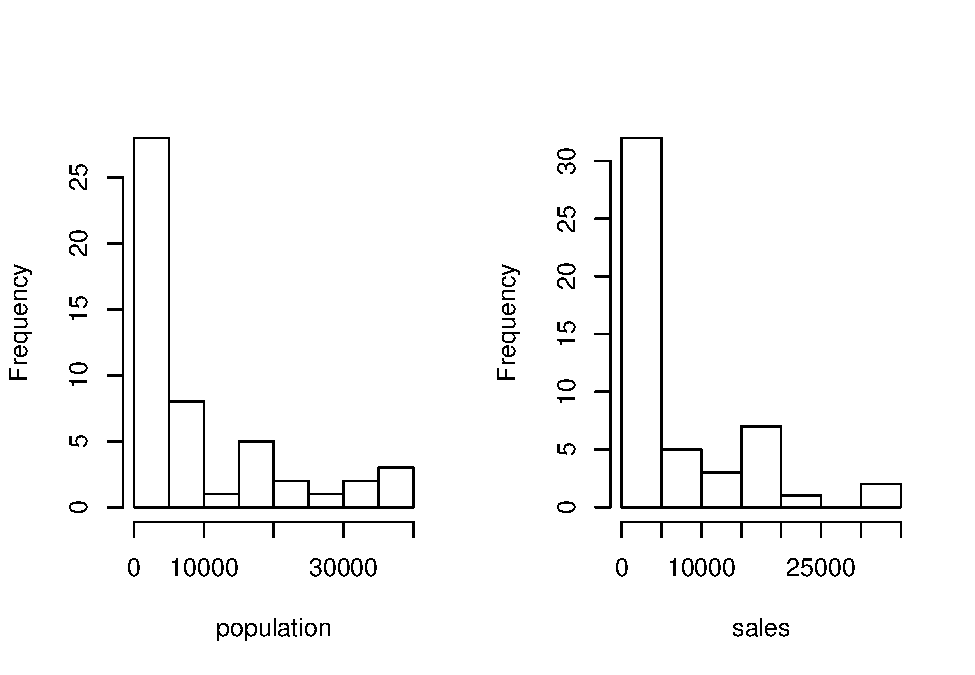
\includegraphics{RegressModelDataCamp_files/figure-latex/unnamed-chunk-45-1.pdf}

Show Overhead D Details. Visualizing relationships with a scatter plot

\hypertarget{toggleOver2.1D}{}
\begin{Shaded}
\begin{Highlighting}[]
\KeywordTok{plot}\NormalTok{(Lot}\OperatorTok{$}\NormalTok{pop, Lot}\OperatorTok{$}\NormalTok{sales, }\DataTypeTok{xlab =} \StringTok{"population"}\NormalTok{, }\DataTypeTok{ylab =} \StringTok{"sales"}\NormalTok{)}
\end{Highlighting}
\end{Shaded}

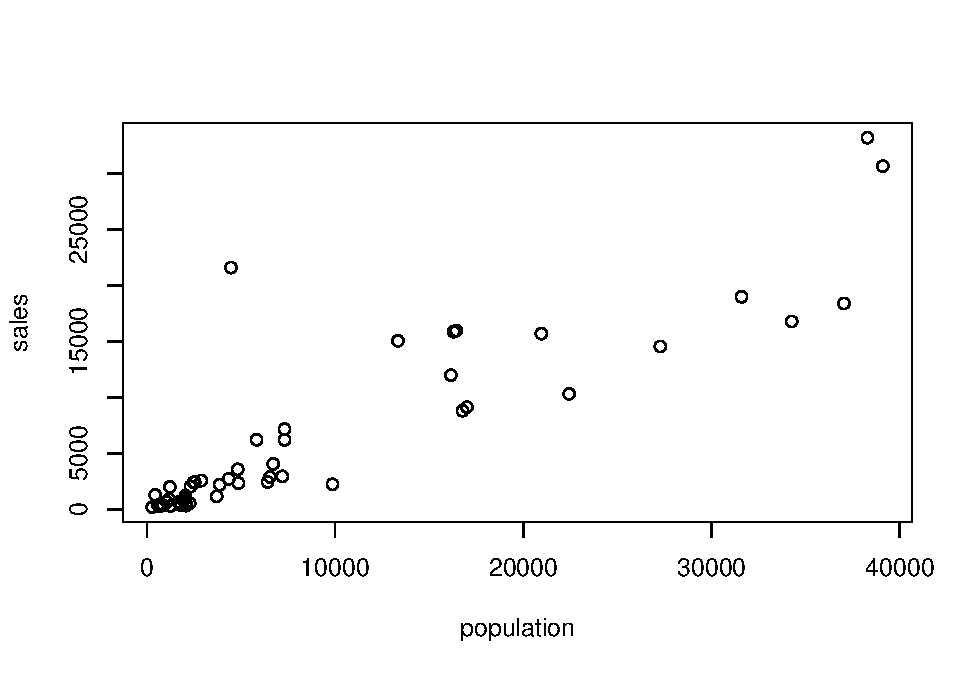
\includegraphics{RegressModelDataCamp_files/figure-latex/unnamed-chunk-46-1.pdf}

Show Overhead E Details. Correlation coefficient

\hypertarget{toggleOver2.1E}{}
\begin{Shaded}
\begin{Highlighting}[]
\KeywordTok{cor}\NormalTok{(Lot}\OperatorTok{$}\NormalTok{pop, Lot}\OperatorTok{$}\NormalTok{sales)}
\end{Highlighting}
\end{Shaded}

\begin{verbatim}
[1] 0.8862827
\end{verbatim}

\subsection{Exercise. Correlations and the Wisconsin
lottery}\label{exercise.-correlations-and-the-wisconsin-lottery}

\textbf{Assignment Text}

The Wisconsin lottery dataset, \texttt{Wisc\_lottery},has already been
read into a dataframe \texttt{Lot}.

Like insurance, lotteries are uncertain events and so the skills to work
with and interpret lottery data are readily applicable to insurance. It
is common to report sales and population in thousands of units, so this
exercise gives you practice in rescaling data via linear
transformations.

\textbf{Instructions}

\begin{itemize}
\tightlist
\item
  From the available population and sales variables, create new
  variables in the dataframe \texttt{Lot}, \texttt{pop\_1000} and
  \texttt{sales\_1000} that are in thousands (of people and of dollars,
  respectively).
\item
  Create summary statistics for the dataframe that includes these new
  variables.
\item
  Plot \texttt{pop\_1000} versus \texttt{sales\_1000}.
\item
  Calculate the correlation between \texttt{pop\_1000} versus
  \texttt{sales\_1000} using the function
  \href{https://www.rdocumentation.org/packages/stats/versions/3.5.0/topics/cor}{cor()}.
  How does this differ between the correlation between population and
  sales in the original units?
\end{itemize}

\textbf{Hint.} Use the dataframe to refer to pop and sales as
\texttt{Lot\$pop} and \texttt{Lot\$sales}, respectively

eyJsYW5ndWFnZSI6InIiLCJwcmVfZXhlcmNpc2VfY29kZSI6IiNMb3QgPC0gcmVhZC5jc3YoXCJDU1ZEYXRhXFxcXFdpc2NfbG90dGVyeS5jc3ZcIiwgaGVhZGVyID0gVFJVRSlcbkxvdCA8LSByZWFkLmNzdihcImh0dHBzOi8vYXNzZXRzLmRhdGFjYW1wLmNvbS9wcm9kdWN0aW9uL3JlcG9zaXRvcmllcy8yNjEwL2RhdGFzZXRzL2E3OTJiMzBmYjMyYjA4OTZkZDY4OTQ1MDFjYmFiMzJiNWQ0OGRmNTEvV2lzY19sb3R0ZXJ5LmNzdlwiLCBoZWFkZXIgPSBUUlVFKSIsInNhbXBsZSI6IiMgQ3JlYXRlIG5ldyB2YXJpYWJsZXMsIHNheSwgYHBvcF8xMDAwYCBhbmQgYHNhbGVzXzEwMDBgXG5Mb3QkcG9wXzEwMDAgPC0gX19fXG5fX18gPC0gTG90JHNhbGVzLzEwMDBcblxuIyBDcmVhdGUgc3VtbWFyeSBzdGF0aXN0aWNzIGZvciB0aGUgZGF0YWZyYW1lXG5zdW1tYXJ5KF9fXylcblxuIyBQbG90IGBwb3BfMTAwMGAgdmVyc3VzIGBzYWxlc18xMDAwYC5cbnBsb3QoX19fLCBfX18pXG5cbiMgQ2FsY3VsYXRlIHRoZSBjb3JyZWxhdGlvbiBiZXR3ZWVuIGBwb3BfMTAwMGAgdmVyc3VzIGBzYWxlc18xMDAwYCBcbmNvcihfX18sIF9fXykiLCJzb2x1dGlvbiI6IkxvdCRwb3BfMTAwMCA8LSBMb3QkcG9wLzEwMDBcbkxvdCRzYWxlc18xMDAwIDwtIExvdCRzYWxlcy8xMDAwXG5zdW1tYXJ5KExvdClcbnBsb3QoTG90JHBvcF8xMDAwLCBMb3Qkc2FsZXNfMTAwMClcbmNvcihMb3QkcG9wXzEwMDAsIExvdCRzYWxlc18xMDAwKSIsInNjdCI6ImV4KCkgJT4lIGNoZWNrX29iamVjdChcIkxvdFwiKSAlPiUge1xuICBjaGVja19jb2x1bW4oLiwgXCJwb3BfMTAwMFwiKSAlPiUgY2hlY2tfZXF1YWwoKVxuICBjaGVja19jb2x1bW4oLiwgXCJzYWxlc18xMDAwXCIpICU+JSBjaGVja19lcXVhbCgpXG59XG5leCgpICU+JSBjaGVja19mdW5jdGlvbihcInN1bW1hcnlcIikgJT4lIGNoZWNrX3Jlc3VsdCgpICU+JSBjaGVja19lcXVhbCgpXG5leCgpICU+JSBjaGVja19mdW5jdGlvbihcInBsb3RcIikgJT4le1xuICBjaGVja19hcmcoLiwgXCJ4XCIpICU+JSBjaGVja19lcXVhbCgpXG4gIGNoZWNrX2FyZyguLCBcInlcIikgJT4lIGNoZWNrX2VxdWFsKClcbn1cbmV4KCkgJT4lIGNoZWNrX2Z1bmN0aW9uKFwiY29yXCIpICU+JSBjaGVja19yZXN1bHQoKSAlPiUgY2hlY2tfZXF1YWwoKVxuc3VjY2Vzc19tc2coXCJDb25ncmF0dWxhdGlvbnMhIFdlIHdpbGwgcmVzY2FsZSBkYXRhIHVzaW5nICdsaW5lYXInIHRyYW5zZm9ybWF0aW9ucyByZWd1bGFybHkuIEluIHBhcnQgd2UgZG8gdGhpcyBmb3IgY29tbXVuaWNhdGluZyBvdXIgYW5hbHlzaXMgdG8gb3RoZXJzLiBBbHNvIGluIHBhcnQsIHRoaXMgaXMgZm9yIG91ciBvd24gY29udmVuaWVuY2UgYXMgaXQgY2FuIGFsbG93IHVzIHRvIHNlZSBwYXR0ZXJucyBtb3JlIHJlYWRpbHkuXCIpIn0=

\section{Method of least squares}\label{method-of-least-squares}

\begin{center}\rule{0.5\linewidth}{\linethickness}\end{center}

In this section, you learn how to:

\begin{itemize}
\tightlist
\item
  Fit a line to data using the method of least squares
\item
  Predict an observation using a least squares fitted line
\end{itemize}

\begin{center}\rule{0.5\linewidth}{\linethickness}\end{center}

\subsection{Video}\label{video-5}

\subsubsection{Video Overheads}\label{video-overheads}

Show Overhead A Details. Where to fit the line?

\hypertarget{toggleOver2.2A}{}
\begin{Shaded}
\begin{Highlighting}[]
\NormalTok{model_blr <-}\StringTok{ }\KeywordTok{lm}\NormalTok{(sales }\OperatorTok{~}\StringTok{ }\NormalTok{pop, }\DataTypeTok{data =}\NormalTok{ Lot)}
\KeywordTok{plot}\NormalTok{(Lot}\OperatorTok{$}\NormalTok{pop, Lot}\OperatorTok{$}\NormalTok{sales,}\DataTypeTok{xlab =} \StringTok{"population"}\NormalTok{, }\DataTypeTok{ylab =} \StringTok{"sales"}\NormalTok{)}
\KeywordTok{abline}\NormalTok{(model_blr, }\DataTypeTok{col=}\StringTok{"blue"}\NormalTok{)}
\KeywordTok{abline}\NormalTok{(}\DecValTok{0}\NormalTok{,}\DecValTok{1}\NormalTok{, }\DataTypeTok{col=}\StringTok{"red"}\NormalTok{)}
\end{Highlighting}
\end{Shaded}

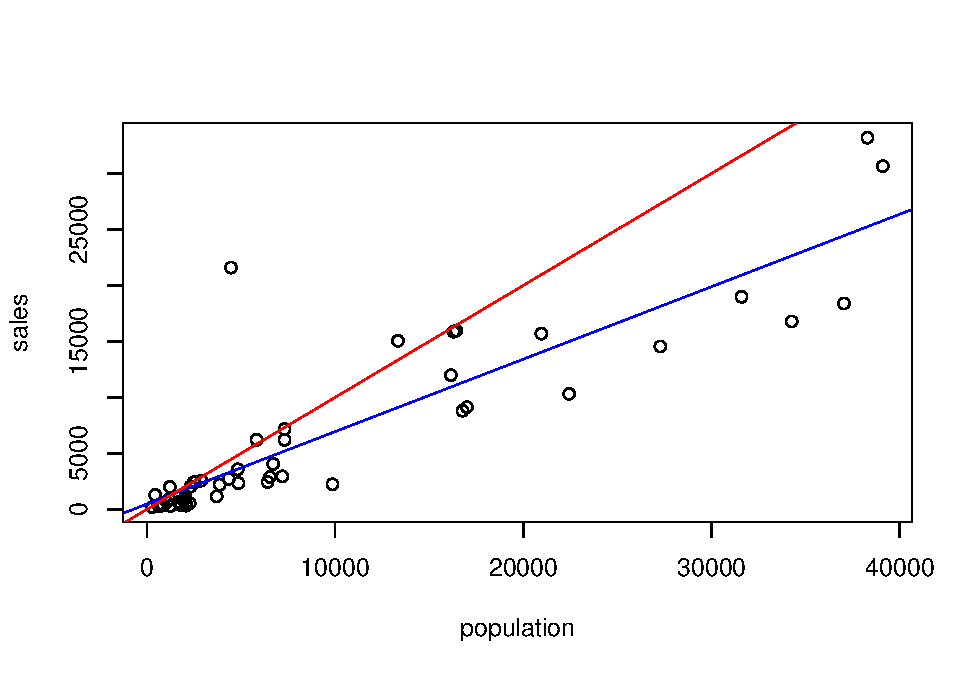
\includegraphics{RegressModelDataCamp_files/figure-latex/unnamed-chunk-52-1.pdf}

Show Overhead B Details. Method of least squares

\hypertarget{toggleOver2.2B}{}
\begin{itemize}
\tightlist
\item
  For observation \(\{(y, x)\}\), the height of the regression line is
  \[b_0 + b_1 x.\]
\item
  Thus, \(y - (b_0 + b_1 x)\) represents the deviation.
\item
  The sum of squared deviations is
  \[SS(b_0, b_1) = \sum (y - (b_0 + b_1 x))^2 .\]
\item
  The \emph{method of least squares} -- determine values of \(b_0, b_1\)
  that minimize \(SS\).
\end{itemize}

Show Overhead C Details. Regression coefficients

\hypertarget{toggleOver2.2C}{}
\begin{Shaded}
\begin{Highlighting}[]
\NormalTok{model_blr <-}\StringTok{ }\KeywordTok{lm}\NormalTok{(sales }\OperatorTok{~}\StringTok{ }\NormalTok{pop, }\DataTypeTok{data =}\NormalTok{ Lot)}
\KeywordTok{round}\NormalTok{(}\KeywordTok{coefficients}\NormalTok{(model_blr), }\DataTypeTok{digits=}\DecValTok{4}\NormalTok{)}
\KeywordTok{plot}\NormalTok{(Lot}\OperatorTok{$}\NormalTok{pop, Lot}\OperatorTok{$}\NormalTok{sales,}\DataTypeTok{xlab =} \StringTok{"population"}\NormalTok{, }\DataTypeTok{ylab =} \StringTok{"sales"}\NormalTok{)}
\KeywordTok{abline}\NormalTok{(model_blr, }\DataTypeTok{col=}\StringTok{"blue"}\NormalTok{)}
\end{Highlighting}
\end{Shaded}

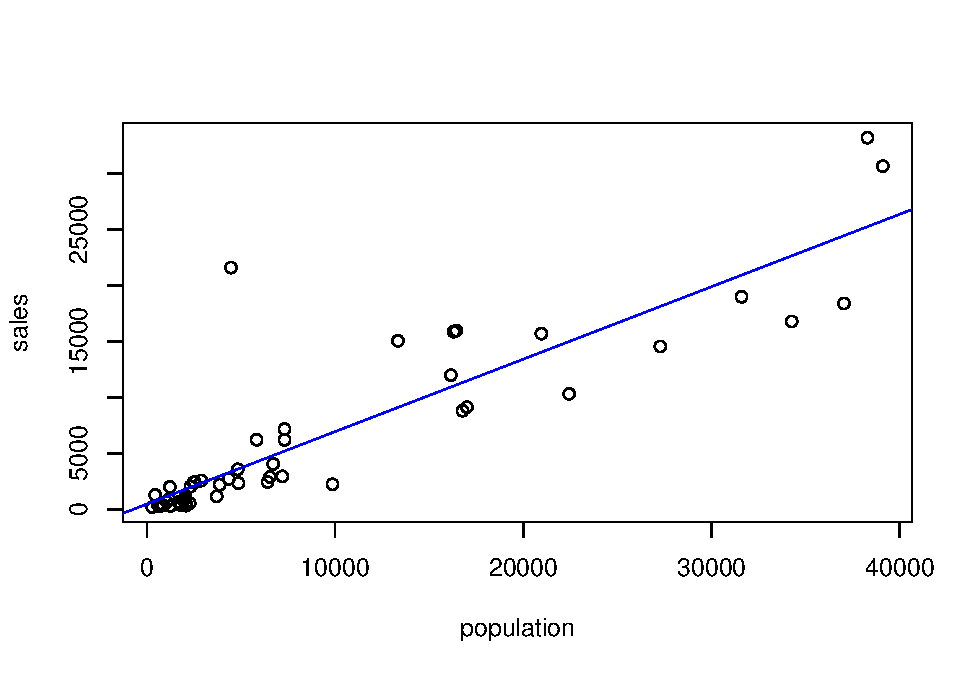
\includegraphics{RegressModelDataCamp_files/figure-latex/unnamed-chunk-53-1.pdf}

\begin{verbatim}
(Intercept)         pop 
   469.7036      0.6471 
\end{verbatim}

Show Overhead D Details. Prediction

\hypertarget{toggleOver2.2D}{}
\begin{Shaded}
\begin{Highlighting}[]
\KeywordTok{round}\NormalTok{(}\KeywordTok{coefficients}\NormalTok{(model_blr), }\DataTypeTok{digits=}\DecValTok{6}\NormalTok{)}
\KeywordTok{coefficients}\NormalTok{(model_blr)[}\DecValTok{1}\NormalTok{] }\OperatorTok{+}\StringTok{ }\KeywordTok{coefficients}\NormalTok{(model_blr)[}\DecValTok{2}\NormalTok{]}\OperatorTok{*}\DecValTok{30000}

\NormalTok{newdata <-}\StringTok{ }\KeywordTok{data.frame}\NormalTok{(}\DataTypeTok{pop =} \DecValTok{30000}\NormalTok{)}
\KeywordTok{predict}\NormalTok{(model_blr, newdata)}
\end{Highlighting}
\end{Shaded}

\begin{verbatim}
(Intercept)         pop 
 469.703598    0.647095 
(Intercept) 
   19882.55 
       1 
19882.55 
\end{verbatim}

\subsection{Exercise. Least squares fit using housing
prices}\label{exercise.-least-squares-fit-using-housing-prices}

\textbf{Assignment Text}

The prior video analyzed the effect that a zip code's population has on
lottery sales. Instead of population, suppose that you wish to
understand the effect that housing prices have on the sale of lottery
tickets. The dataframe \texttt{Lot}, read in from the Wisconsin lottery
dataset \texttt{Wisc\_lottery}, contains the variable \texttt{medhome}
which is the median house price for each zip code, in thousands of
dollars. In this exercise, you will get a feel for the distribution of
this variable by examining summary statistics, examine its relationship
with sales graphically and via correlations, fit a basic linear
regression model and use this model to predict sales.

\textbf{Instructions}

\begin{itemize}
\tightlist
\item
  Summarize the dataframe \texttt{Lot} that contains \texttt{medhome}
  and \texttt{sales}.
\item
  Plot \texttt{medhome} versus \texttt{sales}. Summarize this
  relationship by calculating the corresponding correlation coefficient
  using the function
  \href{https://www.rdocumentation.org/packages/stats/versions/3.5.0/topics/cor}{cor()}.
\item
  Using the function
  \href{https://www.rdocumentation.org/packages/stats/versions/3.5.0/topics/lm}{lm()},
  regress \texttt{medhome}, the explanatory variable, on \texttt{sales},
  the outcome variable. Display the regression coefficients to four
  significant digits.
\item
  Use the function
  \href{https://www.rdocumentation.org/packages/stats/versions/3.5.0/topics/predict}{predict()}
  and the fitted regression model to predict sales assuming that the
  median house price for a zip code is 50 (in thousands of dollars).
\end{itemize}

eyJsYW5ndWFnZSI6InIiLCJwcmVfZXhlcmNpc2VfY29kZSI6IiNMb3QgPC0gcmVhZC5jc3YoXCJDU1ZEYXRhXFxcXFdpc2NfbG90dGVyeS5jc3ZcIiwgaGVhZGVyID0gVFJVRSlcbkxvdCA8LSByZWFkLmNzdihcImh0dHBzOi8vYXNzZXRzLmRhdGFjYW1wLmNvbS9wcm9kdWN0aW9uL3JlcG9zaXRvcmllcy8yNjEwL2RhdGFzZXRzL2E3OTJiMzBmYjMyYjA4OTZkZDY4OTQ1MDFjYmFiMzJiNWQ0OGRmNTEvV2lzY19sb3R0ZXJ5LmNzdlwiLCBoZWFkZXIgPSBUUlVFKSIsInNhbXBsZSI6IiMgU3VtbWFyaXplIHRoZSBkYXRhZnJhbWUgYExvdGAgdGhhdCBjb250YWlucyBgbWVkaG9tZWAgYW5kIGBzYWxlc2BcbnN1bW1hcnkoTG90KVxuIyBQbG90IGFuZCBjYWxjdWxhdGUgdGhlIGNvcnJlbGF0aW9uIG9mIGBtZWRob21lYCB2ZXJzdXMgYHNhbGVzYC4gXG5jb3IoX19fLCBfX18pXG5wbG90KF9fXywgX19fKVxuXG4jIFJlZ3Jlc3MgYG1lZGhvbWVgICBvbiBgc2FsZXNgLiBEaXNwbGF5IHRoZSByZWdyZXNzaW9uIGNvZWZmaWNpZW50cyB0byBmb3VyIHNpZ25pZmljYW50IGRpZ2l0cy5cbm1vZGVsX2JscjEgPC0gbG0oX19fIH4gX19fLCBkYXRhID0gTG90KVxucm91bmQoY29lZmZpY2llbnRzKG1vZGVsX2JscjEpLCBkaWdpdHM9IC0tLSlcblxuIyBQcmVkaWN0IHNhbGVzIGFzc3VtaW5nIHRoYXQgdGhlIG1lZGlhbiBob3VzZSBwcmljZSBpcyA1MCBcbm5ld2RhdGEgPC0gZGF0YS5mcmFtZShtZWRob21lID0gX19fKVxucHJlZGljdChtb2RlbF9ibHIxLCBuZXdkYXRhKSIsInNvbHV0aW9uIjoic3VtbWFyeShMb3QpXG5jb3IoTG90JG1lZGhvbWUsTG90JHNhbGVzKVxucGxvdChMb3QkbWVkaG9tZSxMb3Qkc2FsZXMpXG5tb2RlbF9ibHIxIDwtIGxtKHNhbGVzIH4gbWVkaG9tZSwgZGF0YSA9IExvdClcbnJvdW5kKGNvZWZmaWNpZW50cyhtb2RlbF9ibHIxKSwgZGlnaXRzPTQpXG5uZXdkYXRhIDwtIGRhdGEuZnJhbWUobWVkaG9tZSA9IDUwKVxucHJlZGljdChtb2RlbF9ibHIxLCBuZXdkYXRhKSIsInNjdCI6ImV4KCkgJT4lIGNoZWNrX2Z1bmN0aW9uKFwiY29yXCIpICU+JSBjaGVja19yZXN1bHQoKSAlPiUgY2hlY2tfZXF1YWwoKVxuZXgoKSAlPiUgY2hlY2tfZnVuY3Rpb24oXCJwbG90XCIpICU+JSB7XG4gIGNoZWNrX2FyZyguLCBcInhcIikgJT4lIGNoZWNrX2VxdWFsKClcbiAgY2hlY2tfYXJnKC4sIFwieVwiKSAlPiUgY2hlY2tfZXF1YWwoKVxufVxuZXgoKSAlPiUgY2hlY2tfb2JqZWN0KFwibW9kZWxfYmxyMVwiKSAlPiUgY2hlY2tfZXF1YWwoKVxuZXgoKSAlPiUgY2hlY2tfZnVuY3Rpb24oXCJsbVwiKSAlPiUge1xuICBjaGVja19hcmcoLiwgXCJmb3JtdWxhXCIpICU+JSBjaGVja19lcXVhbCgpXG4gIGNoZWNrX2FyZyguLCBcImRhdGFcIikgJT4lIGNoZWNrX2VxdWFsKClcbn1cbmV4KCkgJT4lIGNoZWNrX2Z1bmN0aW9uKFwicm91bmRcIikgJT4lIHtcbiAgY2hlY2tfYXJnKC4sIFwieFwiKSAlPiUgY2hlY2tfZXF1YWwoKVxuICBjaGVja19hcmcoLiwgXCJkaWdpdHNcIikgJT4lIGNoZWNrX2VxdWFsKClcbn1cbmV4KCkgJT4lIGNoZWNrX29iamVjdChcIm5ld2RhdGFcIikgJT4lIGNoZWNrX2VxdWFsKClcbmV4KCkgJT4lIGNoZWNrX2Z1bmN0aW9uKFwicHJlZGljdFwiKSAlPiUge1xuICBjaGVja19hcmcoLiwgXCJvYmplY3RcIikgJT4lIGNoZWNrX2VxdWFsKClcbiAgY2hlY2tfYXJnKC4sIFwibmV3ZGF0YVwiKSAlPiUgY2hlY2tfZXF1YWwoKVxufVxuc3VjY2Vzc19tc2coXCJDb25ncmF0dWxhdGlvbnMhIFlvdSBub3cgaGF2ZSBleHBlcmllbmNlIGZpdHRpbmcgYSByZWdyZXNzaW9uIGxpbmUgYW5kIHVzaW5nIHRoaXMgbGluZSBmb3IgcHJlZGljdGlvbnMsIGp1c3QgYXMgR2FsdG9uIGRpZCB3aGVuIGhlIHVzZWQgcGFyZW50cycgaGVpZ2h0cyB0byBwcmVkaWN0IHRoZSBoZWlnaHQgb2YgYW4gYWR1bHQgY2hpbGQuIFdlbGwgZG9uZSFcIikifQ==

\section{Understanding variability}\label{understanding-variability}

\begin{center}\rule{0.5\linewidth}{\linethickness}\end{center}

In this section, you learn how to:

\begin{itemize}
\tightlist
\item
  Visualize the ANOVA decomposition of variability
\item
  Calculate and interpret \(R^2\), the coefficient of determination
\item
  Calculate and interpret \(s^2\) the mean square error
\item
  Explain the components of the ANOVA table
\end{itemize}

\begin{center}\rule{0.5\linewidth}{\linethickness}\end{center}

\subsection{Video}\label{video-6}

\subsubsection*{Video Overhead Details}\label{video-overhead-details-5}
\addcontentsline{toc}{subsubsection}{Video Overhead Details}

Show OverheadS A and B Details. Visualizing the uncertainty about a line

\hypertarget{toggleOver2.3A}{}
\begin{Shaded}
\begin{Highlighting}[]
\KeywordTok{par}\NormalTok{(}\DataTypeTok{mar=}\KeywordTok{c}\NormalTok{(}\FloatTok{2.2}\NormalTok{,}\FloatTok{2.1}\NormalTok{,.}\DecValTok{2}\NormalTok{,.}\DecValTok{2}\NormalTok{),}\DataTypeTok{cex=}\FloatTok{1.2}\NormalTok{)}
\NormalTok{x <-}\StringTok{ }\KeywordTok{seq}\NormalTok{(}\OperatorTok{-}\DecValTok{4}\NormalTok{, }\DecValTok{4}\NormalTok{, }\DataTypeTok{len=}\DecValTok{101}\NormalTok{)}
\NormalTok{y <-}\StringTok{ }\NormalTok{x}
\KeywordTok{plot}\NormalTok{(x, y, }\DataTypeTok{type =} \StringTok{"l"}\NormalTok{, }\DataTypeTok{xlim=}\KeywordTok{c}\NormalTok{(}\OperatorTok{-}\DecValTok{3}\NormalTok{, }\DecValTok{4}\NormalTok{), }\DataTypeTok{xaxt=}\StringTok{"n"}\NormalTok{, }\DataTypeTok{yaxt=}\StringTok{"n"}\NormalTok{, }\DataTypeTok{xlab=}\StringTok{""}\NormalTok{, }\DataTypeTok{ylab=}\StringTok{""}\NormalTok{)}
\KeywordTok{axis}\NormalTok{(}\DecValTok{1}\NormalTok{, }\DataTypeTok{at =} \KeywordTok{c}\NormalTok{(}\OperatorTok{-}\DecValTok{1}\NormalTok{, }\DecValTok{1}\NormalTok{),}\DataTypeTok{lab =} \KeywordTok{expression}\NormalTok{(}\KeywordTok{bar}\NormalTok{(x), x))}
\KeywordTok{axis}\NormalTok{(}\DecValTok{2}\NormalTok{, }\DataTypeTok{at =} \KeywordTok{c}\NormalTok{(}\OperatorTok{-}\DecValTok{1}\NormalTok{, }\DecValTok{1}\NormalTok{, }\DecValTok{3}\NormalTok{),}\DataTypeTok{lab =} \KeywordTok{expression}\NormalTok{(}\KeywordTok{bar}\NormalTok{(y), }\KeywordTok{hat}\NormalTok{(y), y), }\DataTypeTok{las=}\DecValTok{1}\NormalTok{)}
\KeywordTok{abline}\NormalTok{(}\OperatorTok{-}\DecValTok{1}\NormalTok{, }\DecValTok{0}\NormalTok{, }\DataTypeTok{lty =} \DecValTok{2}\NormalTok{)}
\KeywordTok{segments}\NormalTok{(}\OperatorTok{-}\DecValTok{4}\NormalTok{, }\DecValTok{1}\NormalTok{, }\DecValTok{1}\NormalTok{, }\DecValTok{1}\NormalTok{, }\DataTypeTok{lty=}\DecValTok{2}\NormalTok{)}
\KeywordTok{segments}\NormalTok{(}\OperatorTok{-}\DecValTok{4}\NormalTok{, }\DecValTok{3}\NormalTok{, }\DecValTok{1}\NormalTok{, }\DecValTok{3}\NormalTok{, }\DataTypeTok{lty =} \DecValTok{2}\NormalTok{)}
\KeywordTok{segments}\NormalTok{(}\DecValTok{1}\NormalTok{, }\OperatorTok{-}\DecValTok{4}\NormalTok{, }\DecValTok{1}\NormalTok{, }\DecValTok{3}\NormalTok{, }\DataTypeTok{lty =} \DecValTok{2}\NormalTok{)}
\KeywordTok{segments}\NormalTok{(}\OperatorTok{-}\DecValTok{1}\NormalTok{, }\OperatorTok{-}\DecValTok{4}\NormalTok{, }\OperatorTok{-}\DecValTok{1}\NormalTok{, }\OperatorTok{-}\DecValTok{1}\NormalTok{, }\DataTypeTok{lty =} \DecValTok{2}\NormalTok{)}

\KeywordTok{points}\NormalTok{(}\DecValTok{1}\NormalTok{, }\DecValTok{3}\NormalTok{, }\DataTypeTok{cex=}\FloatTok{1.5}\NormalTok{, }\DataTypeTok{pch=}\DecValTok{19}\NormalTok{)}

\KeywordTok{arrows}\NormalTok{(}\FloatTok{1.0}\NormalTok{, }\DecValTok{1}\NormalTok{, }\FloatTok{1.0}\NormalTok{, }\DecValTok{3}\NormalTok{, }\DataTypeTok{code =} \DecValTok{3}\NormalTok{, }\DataTypeTok{lty =} \DecValTok{1}\NormalTok{, }\DataTypeTok{angle=}\DecValTok{15}\NormalTok{, }\DataTypeTok{length=}\FloatTok{0.12}\NormalTok{, }\DataTypeTok{lwd=}\DecValTok{2}\NormalTok{)}
\KeywordTok{text}\NormalTok{(}\FloatTok{1.3}\NormalTok{, }\FloatTok{2.2}\NormalTok{,   }\KeywordTok{expression}\NormalTok{( y}\OperatorTok{-}\KeywordTok{hat}\NormalTok{(y)),}\DataTypeTok{cex=}\FloatTok{0.8}\NormalTok{) }
\KeywordTok{text}\NormalTok{(}\OperatorTok{-}\NormalTok{.}\DecValTok{3}\NormalTok{,}\FloatTok{2.2}\NormalTok{,}\StringTok{"'unexplained' deviation"}\NormalTok{, }\DataTypeTok{cex=}\NormalTok{.}\DecValTok{8}\NormalTok{) }
\KeywordTok{arrows}\NormalTok{(}\FloatTok{1.0}\NormalTok{, }\OperatorTok{-}\DecValTok{1}\NormalTok{, }\FloatTok{1.0}\NormalTok{, }\DecValTok{1}\NormalTok{, }\DataTypeTok{code =} \DecValTok{3}\NormalTok{, }\DataTypeTok{lty =} \DecValTok{1}\NormalTok{, }\DataTypeTok{angle=}\DecValTok{15}\NormalTok{, }\DataTypeTok{length=}\FloatTok{0.12}\NormalTok{, }\DataTypeTok{lwd=}\DecValTok{2}\NormalTok{)}
\KeywordTok{text}\NormalTok{(}\FloatTok{1.85}\NormalTok{, }\DecValTok{0}\NormalTok{, }\KeywordTok{expression}\NormalTok{(}\KeywordTok{hat}\NormalTok{(y)}\OperatorTok{-}\KeywordTok{bar}\NormalTok{(y) }\OperatorTok{==}\StringTok{ }\NormalTok{b[}\DecValTok{1}\NormalTok{](x}\OperatorTok{-}\KeywordTok{bar}\NormalTok{(x)) ), }\DataTypeTok{cex=}\FloatTok{0.8}\NormalTok{ )}
\KeywordTok{text}\NormalTok{(}\FloatTok{2.1}\NormalTok{, }\OperatorTok{-}\FloatTok{0.5}\NormalTok{, }\StringTok{" 'explained' deviation"}\NormalTok{, }\DataTypeTok{cex=}\FloatTok{0.8}\NormalTok{)}
\KeywordTok{arrows}\NormalTok{(}\OperatorTok{-}\DecValTok{1}\NormalTok{, }\OperatorTok{-}\FloatTok{1.0}\NormalTok{, }\DecValTok{1}\NormalTok{, }\OperatorTok{-}\FloatTok{1.0}\NormalTok{, }\DataTypeTok{code =} \DecValTok{3}\NormalTok{, }\DataTypeTok{lty =} \DecValTok{1}\NormalTok{, }\DataTypeTok{angle=}\DecValTok{15}\NormalTok{, }\DataTypeTok{length=}\FloatTok{0.12}\NormalTok{, }\DataTypeTok{lwd =} \DecValTok{2}\NormalTok{)}
\KeywordTok{text}\NormalTok{(}\DecValTok{0}\NormalTok{, }\OperatorTok{-}\FloatTok{1.3}\NormalTok{, }\KeywordTok{expression}\NormalTok{( x}\OperatorTok{-}\KeywordTok{bar}\NormalTok{(x)), }\DataTypeTok{cex=}\FloatTok{0.8}\NormalTok{  )}
\KeywordTok{text}\NormalTok{(}\FloatTok{3.5}\NormalTok{, }\FloatTok{2.7}\NormalTok{, }\KeywordTok{expression}\NormalTok{( }\KeywordTok{hat}\NormalTok{(y)}\OperatorTok{==}\StringTok{ }\NormalTok{b[}\DecValTok{0}\NormalTok{]}\OperatorTok{+}\StringTok{ }\NormalTok{b[}\DecValTok{1}\NormalTok{]}\OperatorTok{*}\NormalTok{x), }\DataTypeTok{cex=}\FloatTok{0.8}\NormalTok{  )}
\end{Highlighting}
\end{Shaded}

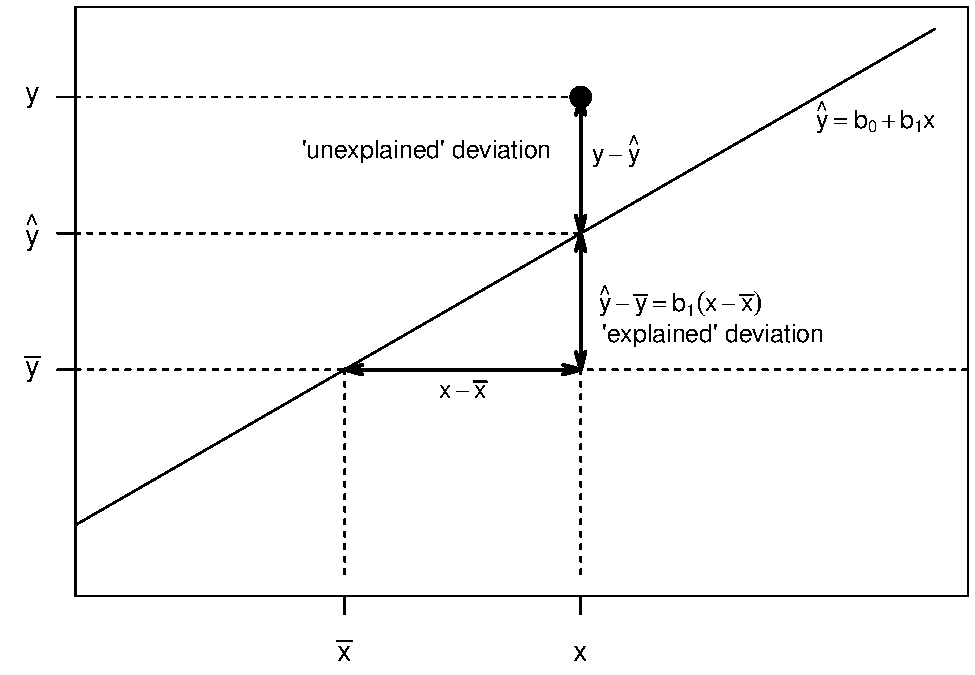
\includegraphics{RegressModelDataCamp_files/figure-latex/unnamed-chunk-59-1.pdf}

Show Overheads C, D and E Details. ANOVA Table

\hypertarget{toggleOver2.3C}{}
\begin{Shaded}
\begin{Highlighting}[]
\NormalTok{model_blr <-}\StringTok{ }\KeywordTok{lm}\NormalTok{(sales }\OperatorTok{~}\StringTok{ }\NormalTok{pop, }\DataTypeTok{data =}\NormalTok{ Lot)}
\KeywordTok{anova}\NormalTok{(model_blr)}
\KeywordTok{sqrt}\NormalTok{(}\KeywordTok{anova}\NormalTok{(model_blr)}\OperatorTok{$}\NormalTok{Mean[}\DecValTok{2}\NormalTok{])}
\KeywordTok{summary}\NormalTok{(model_blr)}\OperatorTok{$}\NormalTok{r.squared}
\end{Highlighting}
\end{Shaded}

\begin{verbatim}
Analysis of Variance Table

Response: sales
          Df     Sum Sq    Mean Sq F value    Pr(>F)    
pop        1 2527165015 2527165015  175.77 < 2.2e-16 ***
Residuals 48  690116755   14377432                      
---
Signif. codes:  0 '***' 0.001 '**' 0.01 '*' 0.05 '.' 0.1 ' ' 1
[1] 3791.758
[1] 0.7854969
\end{verbatim}

\subsection{Exercise. Summarizing measures of
uncertainty}\label{exercise.-summarizing-measures-of-uncertainty}

\textbf{Assignment Text}

In a previous exercise, you developed a regression line to fit the
variable \texttt{medhome}, the median house price for each zip code, as
a predictor of lottery sales. The regression of \texttt{medhome} on
\texttt{sales} has been summarized in the \texttt{R} object
\texttt{model\_blr}.

How reliable is the regression line? In this excercise, you will compute
some of the standard measures that are used to summarize the goodness of
this fit.

\textbf{Instructions}

\begin{itemize}
\tightlist
\item
  Summarize the fitted regression model in an ANOVA table.
\item
  Determine the size of the typical residual, \(s\).
\item
  Determine the coefficient of determination, \(R^2\).
\end{itemize}

\textbf{Hint.} Learn more about possibilities through the
\texttt{Rdocumentation} site. If you have not done so already, check out
the function
\href{https://www.rdocumentation.org/packages/stats/versions/3.5.1/topics/anova}{anova()}

eyJsYW5ndWFnZSI6InIiLCJwcmVfZXhlcmNpc2VfY29kZSI6IiNMb3QgPC0gcmVhZC5jc3YoXCJDU1ZEYXRhXFxcXFdpc2NfbG90dGVyeS5jc3ZcIiwgaGVhZGVyID0gVFJVRSlcbkxvdCA8LSByZWFkLmNzdihcImh0dHBzOi8vYXNzZXRzLmRhdGFjYW1wLmNvbS9wcm9kdWN0aW9uL3JlcG9zaXRvcmllcy8yNjEwL2RhdGFzZXRzL2E3OTJiMzBmYjMyYjA4OTZkZDY4OTQ1MDFjYmFiMzJiNWQ0OGRmNTEvV2lzY19sb3R0ZXJ5LmNzdlwiLCBoZWFkZXIgPSBUUlVFKSIsInNhbXBsZSI6Im1vZGVsX2JsciA8LSBsbShzYWxlcyAgfiBtZWRob21lLCBkYXRhID0gTG90KVxuXG4jIFN1bW1hcml6ZSB0aGUgZml0dGVkIHJlZ3Jlc3Npb24gbW9kZWwgaW4gYW4gQU5PVkEgdGFibGUuXG5hbm92YShfX18pXG5cbiMgRGV0ZXJtaW5lIHRoZSBzaXplIG9mIHRoZSB0eXBpY2FsIHJlc2lkdWFsLCAkcyQuXG5zcXJ0KGFub3ZhKF9fXykkTWVhblsyXSlcblxuIyBEZXRlcm1pbmUgdGhlIGNvZWZmaWNpZW50IG9mIGRldGVybWluYXRpb24sICRSXjIkLiBcbnN1bW1hcnkoX19fKSRyLnNxdWFyZWQiLCJzb2x1dGlvbiI6Im1vZGVsX2JsciA8LSBsbShzYWxlcyAgfiBtZWRob21lLCBkYXRhID0gTG90KVxuYW5vdmEobW9kZWxfYmxyKVxuc3FydChhbm92YShtb2RlbF9ibHIpJE1lYW5bMl0pXG5zdW1tYXJ5KG1vZGVsX2Jscikkci5zcXVhcmVkIiwic2N0IjoiZXgoKSAlPiUgY2hlY2tfb2JqZWN0KFwibW9kZWxfYmxyXCIpICU+JSBjaGVja19lcXVhbCgpXG5leCgpICU+JSBjaGVja19mdW5jdGlvbihcImxtXCIpICU+JSB7XG4gIGNoZWNrX2FyZyguLCBcImZvcm11bGFcIikgJT4lIGNoZWNrX2VxdWFsKClcbiAgY2hlY2tfYXJnKC4sIFwiZGF0YVwiKSAlPiUgY2hlY2tfZXF1YWwoKVxufVxuZXgoKSAlPiUgY2hlY2tfZnVuY3Rpb24oXCJhbm92YVwiKSAlPiUgY2hlY2tfYXJnKFwib2JqZWN0XCIpICU+JSBjaGVja19lcXVhbCgpXG5leCgpICU+JSBjaGVja19mdW5jdGlvbihcInNxcnRcIikgJT4lIGNoZWNrX3Jlc3VsdCgpICU+JSBjaGVja19lcXVhbCgpXG5leCgpICU+JSBjaGVja19mdW5jdGlvbihcInN1bW1hcnlcIikgJT4lIGNoZWNrX3Jlc3VsdCgpICU+JSBjaGVja19lcXVhbCgpXG5zdWNjZXNzX21zZyhcIkNvbmdyYXR1bGF0aW9ucyEgSXQgd2lsbCBiZSBoZWxwZnVsIGlmIHlvdSBjb21wYXJlIHRoZSByZXN1bHRzIG9mIHRoaXMgZXhlcmNpc2UgdG8gdGhlIHJlZ3Jlc3Npb24gb2YgYHBvcGAgb24gYHNhbGVzYCBmcm9tIHRoZSBwcmlvciB2aWRlby4gV2UgaGF2ZSBzZWVuIHRoYXQgYHBvcGAgaXMgbW9yZSBoaWdobHkgY29ycmVsYXRlZCB3aXRoIGBzYWxlc2AgdGhhbiBgbWVkaG9tZWAsIHNvIHdlIGFyZSBleHBlY3RpbmcgZ3JlYXRlciB1bmNlcnRhaW50eSBpbiB0aGlzIHJlZ3Jlc3Npb24gZml0LlwiKSJ9

\subsection{Exercise. Effects of linear transforms on measures of
uncertainty}\label{exercise.-effects-of-linear-transforms-on-measures-of-uncertainty}

\textbf{Assignment Text}

Let us see how rescaling, a linear transformation, affects our measures
of uncertainty. As before, the Wisconsin lottery dataset
\texttt{Wisc\_lottery} has been read into a dataframe \texttt{Lot} that
also contains \texttt{sales\_1000}, sales in thousands of dollars, and
\texttt{pop\_1000}, zip code population in thousands. How do measures of
uncertainty change when going from the original units to thousands of
those units?

\textbf{Instructions}

\begin{itemize}
\tightlist
\item
  Run a regression of \texttt{pop} on \texttt{sales\_1000} and summarize
  this in an ANOVA table.
\item
  For this regression, determine the \(s\) and the coefficient of
  determination, \(R^2\).\\
\item
  Run a regression of \texttt{pop\_1000} on \texttt{sales\_1000} and
  summarize this in an ANOVA table.
\item
  For this regression, determine the \(s\) and the coefficient of
  determination, \(R^2\).
\end{itemize}

\textbf{Hint.} The residual standard error is also available as
\texttt{summary(model\_blr1)\$sigma}. The coefficient of determination
is also available as \texttt{summary(model\_blr1)\$r.squared}.

eyJsYW5ndWFnZSI6InIiLCJwcmVfZXhlcmNpc2VfY29kZSI6IiNMb3QgPC0gcmVhZC5jc3YoXCJDU1ZEYXRhXFxcXFdpc2NfbG90dGVyeS5jc3ZcIiwgaGVhZGVyID0gVFJVRSlcbkxvdCA8LSByZWFkLmNzdihcImh0dHBzOi8vYXNzZXRzLmRhdGFjYW1wLmNvbS9wcm9kdWN0aW9uL3JlcG9zaXRvcmllcy8yNjEwL2RhdGFzZXRzL2E3OTJiMzBmYjMyYjA4OTZkZDY4OTQ1MDFjYmFiMzJiNWQ0OGRmNTEvV2lzY19sb3R0ZXJ5LmNzdlwiLCBoZWFkZXIgPSBUUlVFKVxuTG90JHBvcF8xMDAwIDwtIExvdCRwb3AvMTAwMFxuTG90JHNhbGVzXzEwMDAgPC0gTG90JHNhbGVzLzEwMDAiLCJzYW1wbGUiOiIjIFJ1biBhIHJlZ3Jlc3Npb24gb2YgYHBvcGAgb24gYHNhbGVzXzEwMDBgIGFuZCBzdW1tYXJpemUgdGhpcyBpbiBhbiBBTk9WQSB0YWJsZS5cbm1vZGVsX2JscjEgPC0gbG0oc2FsZXNfMTAwMCAgfiBwb3AsIGRhdGEgPSBMb3QpXG5hbm92YShfX18pXG5cbiMgRGV0ZXJtaW5lIHRoZSAkcyQgYW5kIHRoZSBjb2VmZmljaWVudCBvZiBkZXRlcm1pbmF0aW9uLCAkUl4yJC4gIFxuc3FydChhbm92YShfX18pJE1lYW5bMl0pXG5zdW1tYXJ5KF9fXykkci5zcXVhcmVkXG5cbiMgUnVuIGEgcmVncmVzc2lvbiBvZiBgcG9wXzEwMDBgIG9uIGBzYWxlc18xMDAwYCBhbmQgc3VtbWFyaXplIHRoaXMgaW4gYW4gQU5PVkEgdGFibGUuXG5tb2RlbF9ibHIyIDwtIGxtKF9fXyAgfiBfX18sIGRhdGEgPSBMb3QpXG5hbm92YShtb2RlbF9ibHIyKVxuXG4jIERldGVybWluZSB0aGUgJHMkIGFuZCB0aGUgY29lZmZpY2llbnQgb2YgZGV0ZXJtaW5hdGlvbiwgJFJeMiQuIFxuX19fXG5fX18iLCJzb2x1dGlvbiI6Im1vZGVsX2JscjEgPC0gbG0oc2FsZXNfMTAwMCAgfiBwb3AsIGRhdGEgPSBMb3QpXG5hbm92YShtb2RlbF9ibHIxKVxuc3FydChhbm92YShtb2RlbF9ibHIxKSRNZWFuWzJdKVxuc3VtbWFyeShtb2RlbF9ibHIxKSRyLnNxdWFyZWRcbm1vZGVsX2JscjIgPC0gbG0oc2FsZXNfMTAwMCAgfiBwb3BfMTAwMCAsIGRhdGEgPSBMb3QpXG5hbm92YShtb2RlbF9ibHIyKVxuc3FydChhbm92YShtb2RlbF9ibHIyKSRNZWFuWzJdKVxuc3VtbWFyeShtb2RlbF9ibHIyKSRyLnNxdWFyZWQiLCJzY3QiOiJleCgpICU+JSBjaGVja19vYmplY3QoXCJtb2RlbF9ibHIxXCIpICU+JSBjaGVja19lcXVhbCgpXG5leCgpICU+JSBjaGVja19mdW5jdGlvbihcImFub3ZhXCIsaW5kZXg9MSkgJT4lIGNoZWNrX3Jlc3VsdCgpICU+JSBjaGVja19lcXVhbCgpXG5leCgpICU+JSBjaGVja19mdW5jdGlvbihcInNxcnRcIixpbmRleD0xKSAlPiUgY2hlY2tfcmVzdWx0KCkgJT4lIGNoZWNrX2VxdWFsKClcbmV4KCkgJT4lIGNoZWNrX2Z1bmN0aW9uKFwiYW5vdmFcIixpbmRleD0yKSAlPiUgY2hlY2tfcmVzdWx0KCkgJT4lIGNoZWNrX2VxdWFsKClcbmV4KCkgJT4lIGNoZWNrX2Z1bmN0aW9uKFwic3VtbWFyeVwiLGluZGV4PTEpICU+JSBjaGVja19yZXN1bHQoKSAlPiUgY2hlY2tfZXF1YWwoKVxuZXgoKSAlPiUgY2hlY2tfb2JqZWN0KFwibW9kZWxfYmxyMlwiKSAlPiUgY2hlY2tfZXF1YWwoKVxuZXgoKSAlPiUgY2hlY2tfZnVuY3Rpb24oXCJsbVwiLGluZGV4PTIpICU+JSB7XG4gIGNoZWNrX2FyZyguLCBcImZvcm11bGFcIikgJT4lIGNoZWNrX2VxdWFsKClcbiAgY2hlY2tfYXJnKC4sIFwiZGF0YVwiKSAlPiUgY2hlY2tfZXF1YWwoKVxufVxuZXgoKSAlPiUgY2hlY2tfZnVuY3Rpb24oXCJhbm92YVwiLGluZGV4PTMpICU+JSBjaGVja19yZXN1bHQoKSAlPiUgY2hlY2tfZXF1YWwoKVxuZXgoKSAlPiUgY2hlY2tfZnVuY3Rpb24oXCJzcXJ0XCIsaW5kZXg9MikgJT4lIGNoZWNrX3Jlc3VsdCgpICU+JSBjaGVja19lcXVhbCgpXG5leCgpICU+JSBjaGVja19mdW5jdGlvbihcImFub3ZhXCIsaW5kZXg9NCkgJT4lIGNoZWNrX3Jlc3VsdCgpICU+JSBjaGVja19lcXVhbCgpXG5leCgpICU+JSBjaGVja19mdW5jdGlvbihcInN1bW1hcnlcIixpbmRleD0yKSAlPiUgY2hlY2tfcmVzdWx0KCkgJT4lIGNoZWNrX2VxdWFsKClcbnN1Y2Nlc3NfbXNnKFwiQ29uZ3JhdHVsYXRpb25zISBJbiB0aGlzIGV4ZXJjaXNlLCB5b3UgaGF2ZSBzZWVuIHRoYXQgcmVzY2FsaW5nIGRvZXMgbm90IGFmZmVjdCBvdXIgbWVhc3VyZXMgb2YgZ29vZG5lc3Mgb2YgZml0IGluIGFueSBtZWFuaW5nZnVsIHdheS4gRm9yIGV4YW1wbGUsIGNvZWZmY2llbnQgb2YgZGV0ZXJtaW5hdGlvbnMgYXJlIGNvbXBsZXRlbHkgdW5hZmZlY3RlZC4gVGhpcyBpcyBoZWxwZnVsIGJlY2F1c2Ugd2Ugd2lsbCByZXNjYWxlIHZhcmlhYmxlcyBleHRlbnNpdmVseSBpbiBvdXIgc2VhcmNoIGZvciBwYXR0ZXJucyBpbiB0aGUgZGF0YS5cIikifQ==

\section{Statistical inference}\label{statistical-inference}

\begin{center}\rule{0.5\linewidth}{\linethickness}\end{center}

In this section, you learn how to:

\begin{itemize}
\tightlist
\item
  Conduct a hypothesis test for a regression coefficient using either a
  rejection/acceptance procedure or a p-value
\item
  Calculate and interpret a confidence interval for a regression
  coefficient
\item
  Calculate and interpret a prediction interval at a specific value of a
  predictor variable
\end{itemize}

\begin{center}\rule{0.5\linewidth}{\linethickness}\end{center}

\subsection{Video}\label{video-7}

\subsubsection*{Video Overhead Details}\label{video-overhead-details-6}
\addcontentsline{toc}{subsubsection}{Video Overhead Details}

Show Overhead A Details. Summary of basic linear regression model

\hypertarget{toggleOver2.4A}{}
Introduce the output in the \emph{summary} of the basic linear
regression model.

\begin{Shaded}
\begin{Highlighting}[]
\NormalTok{Lot <-}\StringTok{ }\KeywordTok{read.csv}\NormalTok{(}\StringTok{"CSVData}\CharTok{\textbackslash{}\textbackslash{}}\StringTok{Wisc_lottery.csv"}\NormalTok{, }\DataTypeTok{header =} \OtherTok{TRUE}\NormalTok{)}
\CommentTok{#Lot <- read.csv("https://assets.datacamp.com/production/repositories/2610/datasets/a792b30fb32b0896dd6894501cbab32b5d48df51/Wisc_lottery.csv", header = TRUE)}
\CommentTok{#options(scipen = 8, digits = 4)}
\NormalTok{model_blr <-}\StringTok{ }\KeywordTok{lm}\NormalTok{(sales }\OperatorTok{~}\StringTok{ }\NormalTok{pop, }\DataTypeTok{data =}\NormalTok{ Lot)}
\KeywordTok{summary}\NormalTok{(model_blr)}
\end{Highlighting}
\end{Shaded}

\begin{verbatim}

Call:
lm(formula = sales ~ pop, data = Lot)

Residuals:
    Min      1Q  Median      3Q     Max 
-6046.7 -1460.9  -670.5   485.6 18229.5 

Coefficients:
             Estimate Std. Error t value Pr(>|t|)    
(Intercept) 469.70360  702.90619   0.668    0.507    
pop           0.64709    0.04881  13.258   <2e-16 ***
---
Signif. codes:  0 '***' 0.001 '**' 0.01 '*' 0.05 '.' 0.1 ' ' 1

Residual standard error: 3792 on 48 degrees of freedom
Multiple R-squared:  0.7855,    Adjusted R-squared:  0.781 
F-statistic: 175.8 on 1 and 48 DF,  p-value: < 2.2e-16
\end{verbatim}

Show Overhead B Details. Hypothesis testing

\hypertarget{toggleOver2.4B}{}
\begin{verbatim}
> summary(model_blr)$coefficients
            Estimate Std. Error t value  Pr(>|t|)
(Intercept) 469.7036  702.90619  0.6682 5.072e-01
pop           0.6471    0.04881 13.2579 1.158e-17
\end{verbatim}

Show Overhead C Details. Confidence intervals

\hypertarget{toggleOver2.4C}{}
\begin{Shaded}
\begin{Highlighting}[]
\KeywordTok{confint}\NormalTok{(model_blr, }\DataTypeTok{level =}\NormalTok{ .}\DecValTok{90}\NormalTok{)}
\KeywordTok{confint}\NormalTok{(model_blr, }\DataTypeTok{level =}\NormalTok{ .}\DecValTok{95}\NormalTok{)}
\end{Highlighting}
\end{Shaded}

\begin{verbatim}
                     5 %         95 %
(Intercept) -709.2276710 1648.6348666
pop            0.5652327    0.7289569
                   2.5 %     97.5 %
(Intercept) -943.5840183 1882.99121
pop            0.5489596    0.74523
\end{verbatim}

Show Overhead D Details. Confidence intervals check

\hypertarget{toggleOver2.4D}{}
\begin{Shaded}
\begin{Highlighting}[]
\CommentTok{# Just for checking}
\KeywordTok{summary}\NormalTok{(model_blr)}\OperatorTok{$}\NormalTok{coefficients[}\DecValTok{2}\NormalTok{,}\DecValTok{1}\NormalTok{]}
\KeywordTok{summary}\NormalTok{(model_blr)}\OperatorTok{$}\NormalTok{coefficients[}\DecValTok{2}\NormalTok{,}\DecValTok{2}\NormalTok{]}
\KeywordTok{qt}\NormalTok{(.}\DecValTok{975}\NormalTok{, }\DecValTok{48}\NormalTok{)}

\KeywordTok{summary}\NormalTok{(model_blr)}\OperatorTok{$}\NormalTok{coefficients[}\DecValTok{2}\NormalTok{,}\DecValTok{1}\NormalTok{] }\OperatorTok{-}\StringTok{ }
\StringTok{  }\KeywordTok{summary}\NormalTok{(model_blr)}\OperatorTok{$}\NormalTok{coefficients[}\DecValTok{2}\NormalTok{,}\DecValTok{2}\NormalTok{]}\OperatorTok{*}\KeywordTok{qt}\NormalTok{(.}\DecValTok{975}\NormalTok{, }\DecValTok{48}\NormalTok{)}

\KeywordTok{confint}\NormalTok{(model_blr, }\DataTypeTok{level =}\NormalTok{ .}\DecValTok{95}\NormalTok{)}
\KeywordTok{confint}\NormalTok{(model_blr, }\DataTypeTok{level =}\NormalTok{ .}\DecValTok{95}\NormalTok{)}
\end{Highlighting}
\end{Shaded}

\begin{verbatim}
[1] 0.6470948
[1] 0.04880808
[1] 2.010635
[1] 0.5489596
                   2.5 %     97.5 %
(Intercept) -943.5840183 1882.99121
pop            0.5489596    0.74523
                   2.5 %     97.5 %
(Intercept) -943.5840183 1882.99121
pop            0.5489596    0.74523
\end{verbatim}

Show Overhead E Details. Prediction intervals

\hypertarget{toggleOver2.4E}{}
\begin{Shaded}
\begin{Highlighting}[]
\NormalTok{NewData <-}\StringTok{ }\KeywordTok{data.frame}\NormalTok{(}\DataTypeTok{pop =} \DecValTok{10000}\NormalTok{)}
\KeywordTok{predict}\NormalTok{(model_blr, NewData, }\DataTypeTok{interval =} \StringTok{"prediction"}\NormalTok{, }\DataTypeTok{level =}\NormalTok{ .}\DecValTok{90}\NormalTok{)}
\KeywordTok{predict}\NormalTok{(model_blr, NewData, }\DataTypeTok{interval =} \StringTok{"prediction"}\NormalTok{, }\DataTypeTok{level =}\NormalTok{ .}\DecValTok{99}\NormalTok{)}
\end{Highlighting}
\end{Shaded}

\begin{verbatim}
       fit      lwr      upr
1 6940.651 517.4933 13363.81
       fit       lwr      upr
1 6940.651 -3331.214 17212.52
\end{verbatim}

\subsection{Exercise. Statistical inference and Wisconsin
lottery}\label{exercise.-statistical-inference-and-wisconsin-lottery}

\textbf{Assignment Text}

In a previous exercise, you developed a regression line with the
variable \texttt{medhome}, the median house price for each zip code, as
a predictor of lottery sales. The regression of \texttt{medhome} on
\texttt{sales} has been summarized in the \texttt{R} object
\texttt{model\_blr}.

This exercise allows you to practice the standard inferential tasks:
hypothesis testing, confidence intervals, and prediction.

\textbf{Instructions}

\begin{itemize}
\tightlist
\item
  Summarize the regression model and identify the \emph{t}-statistic for
  testing the importance of the regression coefficient associated with
  \texttt{medhome}.
\item
  Use the function
  \href{https://www.rdocumentation.org/packages/stats/versions/3.5.0/topics/confint}{confint()}
  to provide a 95\% confidence interval for the regression coefficient
  associated with \texttt{medhome}.
\item
  Consider a zip code with a median housing price equal to 50 (in
  thousands of dollars). Use the function
  \href{https://www.rdocumentation.org/packages/stats/versions/3.5.0/topics/predict}{predict()}
  to provide a point prediction and a 95\% prediction interval for
  sales.
\end{itemize}

\textbf{Hint.} Taking a {[}summary(){]} of a regression object produces
a new objeect. You can use the {[}str(){]} structure command to learn
more about the new object. Try out a command such as
\texttt{str(summary(model\_blr))}

eyJsYW5ndWFnZSI6InIiLCJwcmVfZXhlcmNpc2VfY29kZSI6IiNMb3QgPC0gcmVhZC5jc3YoXCJDU1ZEYXRhXFxcXFdpc2NfbG90dGVyeS5jc3ZcIiwgaGVhZGVyID0gVFJVRSlcbkxvdCA8LSByZWFkLmNzdihcImh0dHBzOi8vYXNzZXRzLmRhdGFjYW1wLmNvbS9wcm9kdWN0aW9uL3JlcG9zaXRvcmllcy8yNjEwL2RhdGFzZXRzL2E3OTJiMzBmYjMyYjA4OTZkZDY4OTQ1MDFjYmFiMzJiNWQ0OGRmNTEvV2lzY19sb3R0ZXJ5LmNzdlwiLCBoZWFkZXIgPSBUUlVFKSIsInNhbXBsZSI6Im1vZGVsX2JscjEgPC0gbG0oc2FsZXMgfiBtZWRob21lLCBkYXRhID0gTG90KVxuIyBTdW1tYXJpemUgdGhlIHJlZ3Jlc3Npb24gbW9kZWwgYW5kIGlkZW50aWZ5IHRoZSAkdCQtc3RhdGlzdGljIGZvciB0ZXN0aW5nIHRoZSBpbXBvcnRhbmNlIG9mIHRoZSByZWdyZXNzaW9uIGNvZWZmaWNpZW50IGFzc29jaWF0ZWQgd2l0aCBgbWVkaG9tZWAuXG5zdW1tYXJ5KF9fXylcbnN1bW1hcnkoX19fKSRjb2VmZmljaWVudHNcbnN1bW1hcnkoX19fKSRjb2VmZmljaWVudHNbLDNdXG5cbiMgUHJvdmlkZSBhIDk1XFwlIGNvbmZpZGVuY2UgaW50ZXJ2YWwgZm9yIHRoZSByZWdyZXNzaW9uIGNvZWZmaWNpZW50IGFzc29jaWF0ZWQgd2l0aCBgbWVkaG9tZWAuXG5jb25maW50KF9fXywgbGV2ZWwgPSBfX18pXG5cbiMgUHJvdmlkZSBhIHBvaW50IHByZWRpY3Rpb24gYW5kIGEgOTVcXCUgcHJlZGljdGlvbiBpbnRlcnZhbCBmb3Igc2FsZXMuXG5OZXdEYXRhMSA8LSBkYXRhLmZyYW1lKG1lZGhvbWUgPSA1MClcbnByZWRpY3QoX19fLCBOZXdEYXRhMSwgaW50ZXJ2YWwgPSBcInByZWRpY3Rpb25cIiwgbGV2ZWwgPSBfX18pIiwic29sdXRpb24iOiJtb2RlbF9ibHIxIDwtIGxtKHNhbGVzIH4gbWVkaG9tZSwgZGF0YSA9IExvdClcbnN1bW1hcnkobW9kZWxfYmxyMSlcbnN1bW1hcnkobW9kZWxfYmxyMSkkY29lZmZpY2llbnRzXG5zdW1tYXJ5KG1vZGVsX2JscjEpJGNvZWZmaWNpZW50c1ssM11cblxuY29uZmludChtb2RlbF9ibHIxLCBsZXZlbCA9IC45NSlcblxuTmV3RGF0YTEgPC0gZGF0YS5mcmFtZShtZWRob21lID0gNTApXG5wcmVkaWN0KG1vZGVsX2JscjEsIE5ld0RhdGExLCBpbnRlcnZhbCA9IFwicHJlZGljdGlvblwiLCBsZXZlbCA9IC45NSkiLCJzY3QiOiJleCgpICU+JSBjaGVja19vYmplY3QoXCJtb2RlbF9ibHIxXCIpICU+JSBjaGVja19lcXVhbCgpXG5leCgpICU+JSBjaGVja19mdW5jdGlvbihcImxtXCIpICU+JSB7XG4gIGNoZWNrX2FyZyguLCBcImZvcm11bGFcIikgJT4lIGNoZWNrX2VxdWFsKClcbiAgY2hlY2tfYXJnKC4sIFwiZGF0YVwiKSAlPiUgY2hlY2tfZXF1YWwoKVxufVxuZXgoKSAlPiUgY2hlY2tfZnVuY3Rpb24oXCJzdW1tYXJ5XCIsaW5kZXg9MSkgJT4lIGNoZWNrX2FyZyhcIm9iamVjdFwiKSAlPiUgY2hlY2tfZXF1YWwoKVxuZXgoKSAlPiUgY2hlY2tfZnVuY3Rpb24oXCJzdW1tYXJ5XCIsaW5kZXg9MikgJT4lIGNoZWNrX3Jlc3VsdCgpICU+JSBjaGVja19lcXVhbCgpXG5leCgpICU+JSBjaGVja19mdW5jdGlvbihcInN1bW1hcnlcIixpbmRleD0zKSAlPiUgY2hlY2tfcmVzdWx0KCkgJT4lIGNoZWNrX2VxdWFsKClcbmV4KCkgJT4lIGNoZWNrX2Z1bmN0aW9uKFwiY29uZmludFwiKSAlPiUge1xuICBjaGVja19hcmcoLiwgXCJvYmplY3RcIikgJT4lIGNoZWNrX2VxdWFsKClcbiAgY2hlY2tfYXJnKC4sIFwibGV2ZWxcIikgJT4lIGNoZWNrX2VxdWFsKClcbn1cbmV4KCkgJT4lIGNoZWNrX2Z1bmN0aW9uKFwiY29uZmludFwiKSAlPiUgY2hlY2tfcmVzdWx0KCkgJT4lIGNoZWNrX2VxdWFsKClcbmV4KCkgJT4lIGNoZWNrX29iamVjdChcIk5ld0RhdGExXCIpICU+JSBjaGVja19lcXVhbCgpXG5leCgpICU+JSBjaGVja19mdW5jdGlvbihcInByZWRpY3RcIikgJT4lIHtcbiAgY2hlY2tfYXJnKC4sIFwib2JqZWN0XCIpICU+JSBjaGVja19lcXVhbCgpXG4gIGNoZWNrX2FyZyguLCBcIm5ld2RhdGFcIikgJT4lIGNoZWNrX2VxdWFsKClcbiAgY2hlY2tfYXJnKC4sIFwiaW50ZXJ2YWxcIikgJT4lIGNoZWNrX2VxdWFsKClcbiAgY2hlY2tfYXJnKC4sIFwibGV2ZWxcIikgJT4lIGNoZWNrX2VxdWFsKClcbn1cbmV4KCkgJT4lIGNoZWNrX2Z1bmN0aW9uKFwicHJlZGljdFwiKSAlPiUgY2hlY2tfcmVzdWx0KCkgJT4lIGNoZWNrX2VxdWFsKClcbnN1Y2Nlc3NfbXNnKFwiQ29uZ3JhdHVsYXRpb25zISBNdWNoIG9mIHdoYXQgd2UgbGVhcm4gZnJvbSBhIGRhdGEgbW9kZWxpbmcgZXhlcmNpc2UgY2FuIGJlIHN1bW1hcml6ZWQgdXNpbmcgc3RhbmRhcmQgaW5mZXJlbnRpYWwgdG9vbHM6IGh5cG90aGVzaXMgdGVzdGluZywgY29uZmlkZW5jZSBpbnRlcnZhbHMsIGFuZCBwcmVkaWN0aW9uLlwiKSJ9

\section{Diagnostics}\label{diagnostics}

\begin{center}\rule{0.5\linewidth}{\linethickness}\end{center}

In this section, you learn how to:

\begin{itemize}
\tightlist
\item
  Describe how diagnostic checking and residual analysis are used in a
  statistical analysis
\item
  Describe several model misspecifications commonly encountered in a
  regression analysis
\end{itemize}

\begin{center}\rule{0.5\linewidth}{\linethickness}\end{center}

\subsection{Video}\label{video-8}

\subsubsection*{Video Overhead Details}\label{video-overhead-details-7}
\addcontentsline{toc}{subsubsection}{Video Overhead Details}

Show Overhead A Details. Unusual observations in regression

\hypertarget{toggleOver2.5A}{}
\begin{itemize}
\tightlist
\item
  We have defined regression estimates as minimizers of a least squares
  objective function.
\item
  An appealing intuitive feature of linear regressions is that
  regression estimates can be expressed as weighted averages of
  outcomes.
\item
  The weights vary by observation, some observations are more important
  than others.
\item
  ``Unusual'' observations are far from the majority of the data set:
\item
  Unusual in the vertical direction is called an \emph{outlier}.
\item
  Unusual in the horizontal directional is called a \emph{high leverage
  point}.
\end{itemize}

Show Overhead B Details. Example. Outliers and High Leverage Points

\hypertarget{toggleOver2.5B}{}
\begin{Shaded}
\begin{Highlighting}[]
\NormalTok{outlr <-}\StringTok{ }\KeywordTok{read.csv}\NormalTok{(}\StringTok{"CSVData}\CharTok{\textbackslash{}\textbackslash{}}\StringTok{Outlier.csv"}\NormalTok{, }\DataTypeTok{header =} \OtherTok{TRUE}\NormalTok{)}

\CommentTok{#  FIGURE 2.7}
\KeywordTok{plot}\NormalTok{(outlr}\OperatorTok{$}\NormalTok{x, outlr}\OperatorTok{$}\NormalTok{y, }\DataTypeTok{xlim =} \KeywordTok{c}\NormalTok{(}\DecValTok{0}\NormalTok{, }\DecValTok{10}\NormalTok{), }\DataTypeTok{ylim =} \KeywordTok{c}\NormalTok{(}\DecValTok{2}\NormalTok{, }\DecValTok{9}\NormalTok{), }\DataTypeTok{xlab =} \StringTok{"x"}\NormalTok{, }\DataTypeTok{ylab =} \StringTok{"y"}\NormalTok{)}
\KeywordTok{text}\NormalTok{(}\FloatTok{4.5}\NormalTok{, }\FloatTok{8.0}\NormalTok{, }\StringTok{"A"}\NormalTok{)}
\KeywordTok{text}\NormalTok{(}\FloatTok{9.8}\NormalTok{, }\FloatTok{8.0}\NormalTok{, }\StringTok{"B"}\NormalTok{)}
\KeywordTok{text}\NormalTok{(}\FloatTok{9.8}\NormalTok{, }\FloatTok{2.5}\NormalTok{, }\StringTok{"C"}\NormalTok{)}
\end{Highlighting}
\end{Shaded}

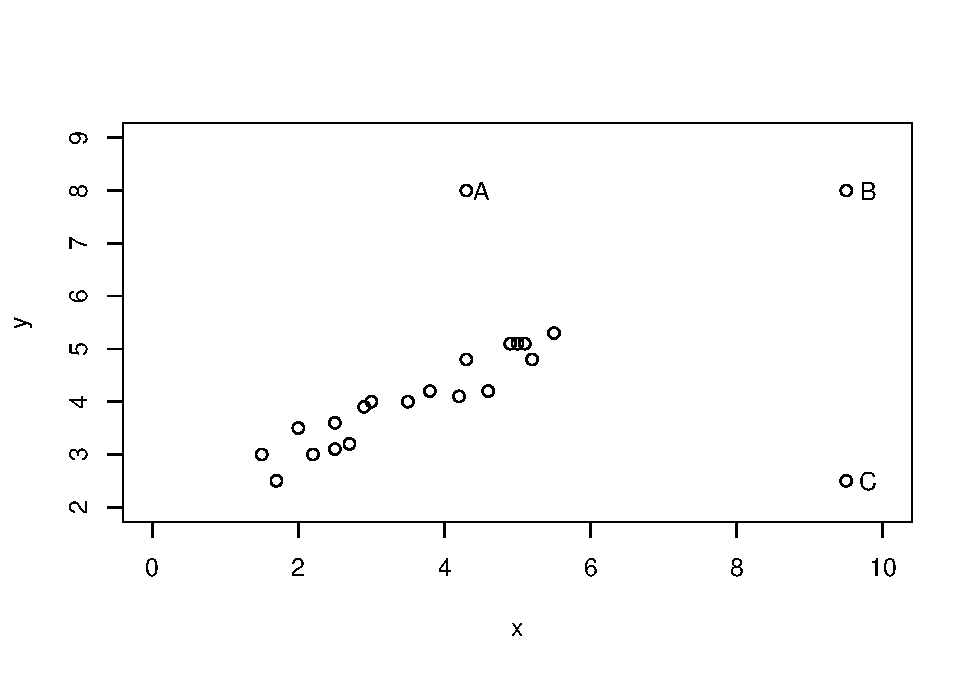
\includegraphics{RegressModelDataCamp_files/figure-latex/unnamed-chunk-77-1.pdf}

Show Overhead C Details. Regression fit with 19 base observations

\hypertarget{toggleOver2.5C}{}
\begin{Shaded}
\begin{Highlighting}[]
\NormalTok{model_outlr0 <-}\StringTok{ }\KeywordTok{lm}\NormalTok{(y }\OperatorTok{~}\StringTok{ }\NormalTok{x, }\DataTypeTok{data =}\NormalTok{ outlr, }\DataTypeTok{subset =} \OperatorTok{-}\KeywordTok{c}\NormalTok{(}\DecValTok{20}\NormalTok{,}\DecValTok{21}\NormalTok{,}\DecValTok{22}\NormalTok{))}
\KeywordTok{summary}\NormalTok{(model_outlr0)}
\KeywordTok{plot}\NormalTok{(outlr}\OperatorTok{$}\NormalTok{x[}\DecValTok{1}\OperatorTok{:}\DecValTok{19}\NormalTok{], outlr}\OperatorTok{$}\NormalTok{y[}\DecValTok{1}\OperatorTok{:}\DecValTok{19}\NormalTok{], }\DataTypeTok{xlab =} \StringTok{"x"}\NormalTok{, }\DataTypeTok{ylab =} \StringTok{"y"}\NormalTok{, }\DataTypeTok{xlim =} \KeywordTok{c}\NormalTok{(}\DecValTok{0}\NormalTok{, }\DecValTok{10}\NormalTok{), }\DataTypeTok{ylim =} \KeywordTok{c}\NormalTok{(}\DecValTok{2}\NormalTok{, }\DecValTok{9}\NormalTok{))}
\KeywordTok{abline}\NormalTok{(model_outlr0)}
\end{Highlighting}
\end{Shaded}

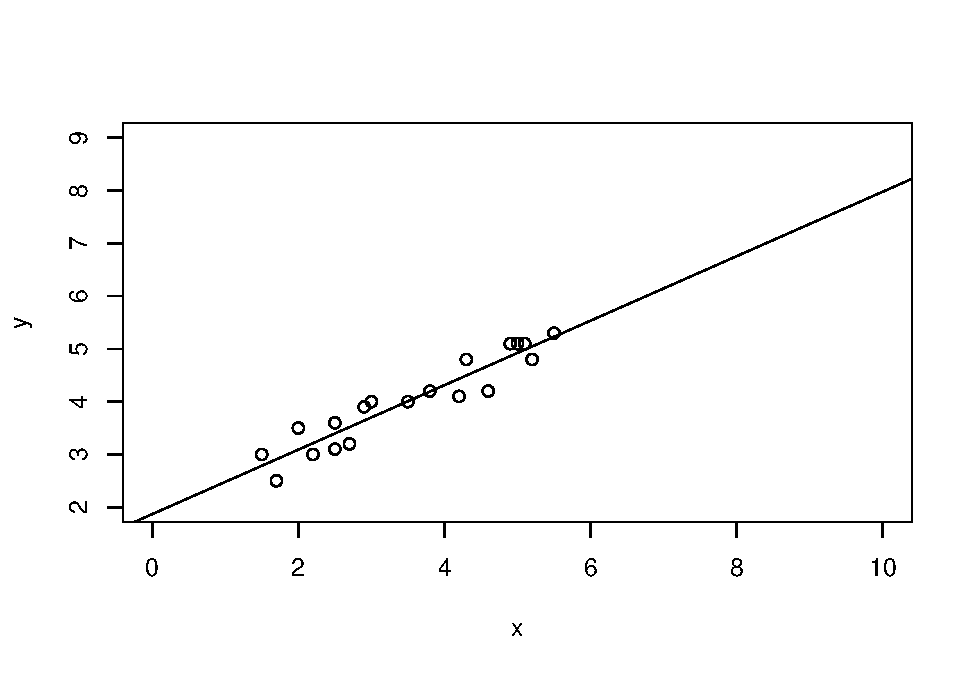
\includegraphics{RegressModelDataCamp_files/figure-latex/unnamed-chunk-78-1.pdf}

\begin{verbatim}

Call:
lm(formula = y ~ x, data = outlr, subset = -c(20, 21, 22))

Residuals:
    Min      1Q  Median      3Q     Max 
-0.4790 -0.2708  0.0711  0.2263  0.4094 

Coefficients:
            Estimate Std. Error t value Pr(>|t|)    
(Intercept)  1.86874    0.19583   9.543 3.06e-08 ***
x            0.61094    0.05219  11.705 1.47e-09 ***
---
Signif. codes:  0 '***' 0.001 '**' 0.01 '*' 0.05 '.' 0.1 ' ' 1

Residual standard error: 0.2883 on 17 degrees of freedom
Multiple R-squared:  0.8896,    Adjusted R-squared:  0.8831 
F-statistic:   137 on 1 and 17 DF,  p-value: 1.471e-09
\end{verbatim}

Show Overhead D Details. Regression fit with 19 base observations plus C

\hypertarget{toggleOver2.5D}{}
\begin{Shaded}
\begin{Highlighting}[]
\NormalTok{model_outlrC <-}\StringTok{ }\KeywordTok{lm}\NormalTok{(y }\OperatorTok{~}\StringTok{ }\NormalTok{x, }\DataTypeTok{data =}\NormalTok{ outlr, }\DataTypeTok{subset =} \OperatorTok{-}\KeywordTok{c}\NormalTok{(}\DecValTok{20}\NormalTok{,}\DecValTok{21}\NormalTok{))}
\KeywordTok{summary}\NormalTok{(model_outlrC)}
\KeywordTok{plot}\NormalTok{(outlr}\OperatorTok{$}\NormalTok{x[}\KeywordTok{c}\NormalTok{(}\DecValTok{1}\OperatorTok{:}\DecValTok{19}\NormalTok{,}\DecValTok{22}\NormalTok{)], outlr}\OperatorTok{$}\NormalTok{y[}\KeywordTok{c}\NormalTok{(}\DecValTok{1}\OperatorTok{:}\DecValTok{19}\NormalTok{,}\DecValTok{22}\NormalTok{)], }\DataTypeTok{xlab =} \StringTok{"x"}\NormalTok{, }\DataTypeTok{ylab =} \StringTok{"y"}\NormalTok{, }\DataTypeTok{xlim =} \KeywordTok{c}\NormalTok{(}\DecValTok{0}\NormalTok{, }\DecValTok{10}\NormalTok{), }\DataTypeTok{ylim =} \KeywordTok{c}\NormalTok{(}\DecValTok{2}\NormalTok{, }\DecValTok{9}\NormalTok{))}
\KeywordTok{text}\NormalTok{(}\FloatTok{9.8}\NormalTok{, }\FloatTok{2.5}\NormalTok{, }\StringTok{"C"}\NormalTok{, }\DataTypeTok{col =} \StringTok{"blue"}\NormalTok{)}
\KeywordTok{abline}\NormalTok{(model_outlrC)}
\end{Highlighting}
\end{Shaded}

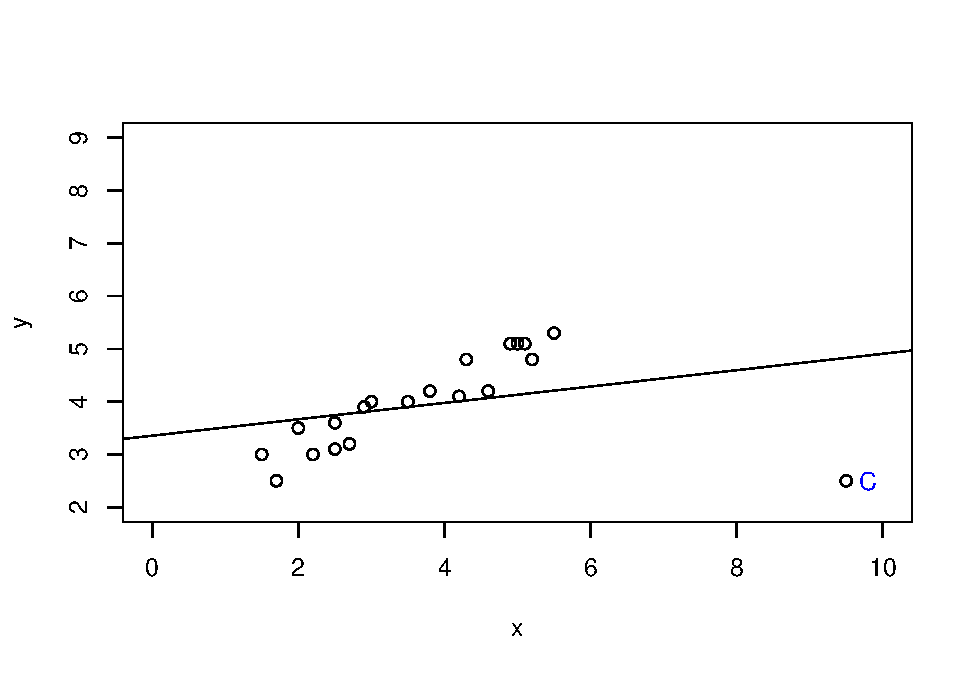
\includegraphics{RegressModelDataCamp_files/figure-latex/unnamed-chunk-79-1.pdf}

\begin{verbatim}

Call:
lm(formula = y ~ x, data = outlr, subset = -c(20, 21))

Residuals:
     Min       1Q   Median       3Q      Max 
-2.32947 -0.57819  0.09772  0.67240  1.09097 

Coefficients:
            Estimate Std. Error t value Pr(>|t|)    
(Intercept)   3.3559     0.4560   7.360 7.87e-07 ***
x             0.1551     0.1078   1.439    0.167    
---
Signif. codes:  0 '***' 0.001 '**' 0.01 '*' 0.05 '.' 0.1 ' ' 1

Residual standard error: 0.8648 on 18 degrees of freedom
Multiple R-squared:  0.1031,    Adjusted R-squared:  0.0533 
F-statistic:  2.07 on 1 and 18 DF,  p-value: 0.1674
\end{verbatim}

Show Overhead E Details. R code

\hypertarget{toggleOver2.5E}{}
\begin{Shaded}
\begin{Highlighting}[]
\NormalTok{model_outlr0 <-}\StringTok{ }\KeywordTok{lm}\NormalTok{(y }\OperatorTok{~}\StringTok{ }\NormalTok{x, }\DataTypeTok{data =}\NormalTok{ outlr, }\DataTypeTok{subset =} \OperatorTok{-}\KeywordTok{c}\NormalTok{(}\DecValTok{20}\NormalTok{,}\DecValTok{21}\NormalTok{,}\DecValTok{22}\NormalTok{))}
\KeywordTok{summary}\NormalTok{(model_outlr0)}
\NormalTok{model_outlrA <-}\StringTok{ }\KeywordTok{lm}\NormalTok{(y }\OperatorTok{~}\StringTok{ }\NormalTok{x, }\DataTypeTok{data =}\NormalTok{ outlr, }\DataTypeTok{subset =} \OperatorTok{-}\KeywordTok{c}\NormalTok{(}\DecValTok{21}\NormalTok{,}\DecValTok{22}\NormalTok{))}
\KeywordTok{summary}\NormalTok{(model_outlrA)}
\NormalTok{model_outlrB <-}\StringTok{ }\KeywordTok{lm}\NormalTok{(y }\OperatorTok{~}\StringTok{ }\NormalTok{x, }\DataTypeTok{data =}\NormalTok{ outlr, }\DataTypeTok{subset =} \OperatorTok{-}\KeywordTok{c}\NormalTok{(}\DecValTok{20}\NormalTok{,}\DecValTok{22}\NormalTok{))}
\KeywordTok{summary}\NormalTok{(model_outlrB)}
\NormalTok{model_outlrC <-}\StringTok{ }\KeywordTok{lm}\NormalTok{(y }\OperatorTok{~}\StringTok{ }\NormalTok{x, }\DataTypeTok{data =}\NormalTok{ outlr, }\DataTypeTok{subset =} \OperatorTok{-}\KeywordTok{c}\NormalTok{(}\DecValTok{20}\NormalTok{,}\DecValTok{21}\NormalTok{))}
\KeywordTok{summary}\NormalTok{(model_outlrC)}
\end{Highlighting}
\end{Shaded}

\begin{verbatim}

Call:
lm(formula = y ~ x, data = outlr, subset = -c(20, 21, 22))

Residuals:
    Min      1Q  Median      3Q     Max 
-0.4790 -0.2708  0.0711  0.2263  0.4094 

Coefficients:
            Estimate Std. Error t value Pr(>|t|)    
(Intercept)  1.86874    0.19583   9.543 3.06e-08 ***
x            0.61094    0.05219  11.705 1.47e-09 ***
---
Signif. codes:  0 '***' 0.001 '**' 0.01 '*' 0.05 '.' 0.1 ' ' 1

Residual standard error: 0.2883 on 17 degrees of freedom
Multiple R-squared:  0.8896,    Adjusted R-squared:  0.8831 
F-statistic:   137 on 1 and 17 DF,  p-value: 1.471e-09


Call:
lm(formula = y ~ x, data = outlr, subset = -c(21, 22))

Residuals:
    Min      1Q  Median      3Q     Max 
-0.7391 -0.3928 -0.1805  0.1225  3.2689 

Coefficients:
            Estimate Std. Error t value Pr(>|t|)    
(Intercept)   1.7500     0.5736   3.051 0.006883 ** 
x             0.6933     0.1517   4.570 0.000237 ***
---
Signif. codes:  0 '***' 0.001 '**' 0.01 '*' 0.05 '.' 0.1 ' ' 1

Residual standard error: 0.8455 on 18 degrees of freedom
Multiple R-squared:  0.5371,    Adjusted R-squared:  0.5114 
F-statistic: 20.89 on 1 and 18 DF,  p-value: 0.0002374


Call:
lm(formula = y ~ x, data = outlr, subset = -c(20, 22))

Residuals:
     Min       1Q   Median       3Q      Max 
-0.51763 -0.28094  0.03452  0.23586  0.44581 

Coefficients:
            Estimate Std. Error t value Pr(>|t|)    
(Intercept)  1.77463    0.15020   11.81 6.48e-10 ***
x            0.63978    0.03551   18.02 5.81e-13 ***
---
Signif. codes:  0 '***' 0.001 '**' 0.01 '*' 0.05 '.' 0.1 ' ' 1

Residual standard error: 0.2849 on 18 degrees of freedom
Multiple R-squared:  0.9474,    Adjusted R-squared:  0.9445 
F-statistic: 324.5 on 1 and 18 DF,  p-value: 5.808e-13


Call:
lm(formula = y ~ x, data = outlr, subset = -c(20, 21))

Residuals:
     Min       1Q   Median       3Q      Max 
-2.32947 -0.57819  0.09772  0.67240  1.09097 

Coefficients:
            Estimate Std. Error t value Pr(>|t|)    
(Intercept)   3.3559     0.4560   7.360 7.87e-07 ***
x             0.1551     0.1078   1.439    0.167    
---
Signif. codes:  0 '***' 0.001 '**' 0.01 '*' 0.05 '.' 0.1 ' ' 1

Residual standard error: 0.8648 on 18 degrees of freedom
Multiple R-squared:  0.1031,    Adjusted R-squared:  0.0533 
F-statistic:  2.07 on 1 and 18 DF,  p-value: 0.1674
\end{verbatim}

Show Overhead F Details. Visualizing four regression fits

\hypertarget{toggleOver2.5F}{}
\begin{Shaded}
\begin{Highlighting}[]
\KeywordTok{plot}\NormalTok{(outlr}\OperatorTok{$}\NormalTok{x, outlr}\OperatorTok{$}\NormalTok{y, }\DataTypeTok{xlim =} \KeywordTok{c}\NormalTok{(}\DecValTok{0}\NormalTok{, }\DecValTok{10}\NormalTok{), }\DataTypeTok{ylim =} \KeywordTok{c}\NormalTok{(}\DecValTok{2}\NormalTok{, }\DecValTok{9}\NormalTok{), }\DataTypeTok{xlab =} \StringTok{"x"}\NormalTok{, }\DataTypeTok{ylab =} \StringTok{"y"}\NormalTok{)}
\KeywordTok{text}\NormalTok{(}\FloatTok{4.5}\NormalTok{, }\FloatTok{8.0}\NormalTok{, }\StringTok{"A"}\NormalTok{, }\DataTypeTok{col =} \StringTok{"red"}\NormalTok{)}
\KeywordTok{text}\NormalTok{(}\FloatTok{9.8}\NormalTok{, }\FloatTok{8.0}\NormalTok{, }\StringTok{"B"}\NormalTok{, }\DataTypeTok{col =} \StringTok{"green"}\NormalTok{)}
\KeywordTok{text}\NormalTok{(}\FloatTok{9.8}\NormalTok{, }\FloatTok{2.5}\NormalTok{, }\StringTok{"C"}\NormalTok{, }\DataTypeTok{col =} \StringTok{"blue"}\NormalTok{)}
\KeywordTok{abline}\NormalTok{(model_outlr0)}
\KeywordTok{abline}\NormalTok{(model_outlrA, }\DataTypeTok{col =} \StringTok{"red"}\NormalTok{)}
\KeywordTok{abline}\NormalTok{(model_outlrB, }\DataTypeTok{col =} \StringTok{"green"}\NormalTok{)}
\KeywordTok{abline}\NormalTok{(model_outlrC, }\DataTypeTok{col =} \StringTok{"blue"}\NormalTok{)}
\end{Highlighting}
\end{Shaded}

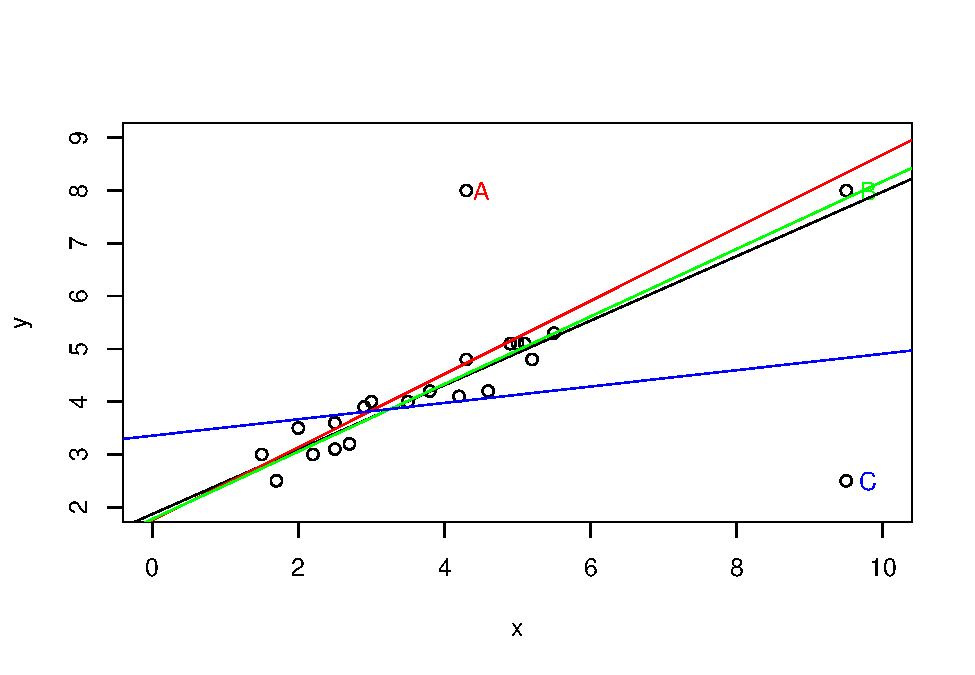
\includegraphics{RegressModelDataCamp_files/figure-latex/unnamed-chunk-81-1.pdf}

Show Overhead G Details. Results from four regression models

\hypertarget{toggleOver2.5G}{}
\[\begin{matrix}
\begin{array}{c}
\text{Results from Four Regressions}
\end{array}\\\scriptsize
\begin{array}{l|rrrrr} \hline \text{Data} & b_0 & b_1 & s & R^2(\%) & t(b_1) \\ \hline \text{19 Base Points} & 1.869 & 0.611 & 0.288 & 89.0 & 11.71 \\ \text{19 Base Points} ~+~ A & 1.750 & 0.693 & 0.846 & 53.7 & 4.57 \\ \text{19 Base Points} ~+~ B & 1.775 & 0.640 & 0.285 & 94.7 & 18.01 \\ \text{19 Base Points} ~+~ C & 3.356 & 0.155 & 0.865 & 10.3 & 1.44 \\ \hline \end{array} 
\end{matrix}\]

\subsection{Exercise. Assessing outliers in lottery
sales}\label{exercise.-assessing-outliers-in-lottery-sales}

\textbf{Assignment Text}

In an earlier video, we made a scatter plot of population versus sales.
This plot exhibits an outlier; the point in the upper left-hand side of
the plot represents a zip code that includes Kenosha, Wisconsin. Sales
for this zip code are unusually high given its population.

This exercise summarizes the regression fit both with and without this
zip code in order to see how robust our results are to the inclusion of
this unusual observation.

\textbf{Instructions}

\begin{itemize}
\tightlist
\item
  A basic linear regression fit of population on sales has already been
  fit in the object \texttt{model\_blr}. Re-fit this same model to the
  data, this time omitting Kenosha (observation number 9).
\item
  Plot these two least squares fitted lines superimposed on the full
  data set.
\item
  What is the effect on the distribution of residuals by removing this
  point? Calculate a normal qq plot with and without Kenosha.
\end{itemize}

\textbf{Hint.} You can extract the residuals from a regression object
with the function {[}residuals(){]}.

eyJsYW5ndWFnZSI6InIiLCJwcmVfZXhlcmNpc2VfY29kZSI6IiNMb3QgPC0gcmVhZC5jc3YoXCJDU1ZEYXRhXFxcXFdpc2NfbG90dGVyeS5jc3ZcIiwgaGVhZGVyID0gVFJVRSlcbkxvdCA8LSByZWFkLmNzdihcImh0dHBzOi8vYXNzZXRzLmRhdGFjYW1wLmNvbS9wcm9kdWN0aW9uL3JlcG9zaXRvcmllcy8yNjEwL2RhdGFzZXRzL2E3OTJiMzBmYjMyYjA4OTZkZDY4OTQ1MDFjYmFiMzJiNWQ0OGRmNTEvV2lzY19sb3R0ZXJ5LmNzdlwiLCBoZWFkZXIgPSBUUlVFKSIsInNhbXBsZSI6Im1vZGVsX2JsciA8LWxtKHNhbGVzIH4gcG9wLCBkYXRhID0gTG90KVxuc3VtbWFyeShtb2RlbF9ibHIpXG4jIFJlLWZpdCB0aGlzIG1vZGVsIHRvIHRoZSBkYXRhLCB0aGlzIHRpbWUgb21pdHRpbmcgS2Vub3NoYSAob2JzZXJ2YXRpb24gbnVtYmVyIDkpLlxubW9kZWxfS2Vub3NoYSA8LSBsbShfX18gfiBfX18sIGRhdGEgPSBMb3QsIHN1YnNldCA9IC1jKDkpKVxuc3VtbWFyeShfX18pXG5cbiMgUGxvdCB0aGVzZSB0d28gbGVhc3Qgc3F1YXJlcyBmaXR0ZWQgbGluZXMgc3VwZXJpbXBvc2VkIG9uIHRoZSBmdWxsIGRhdGEgc2V0LlxucGxvdChfX18sIF9fXywgeGxhYiA9IFwicG9wdWxhdGlvblwiLCB5bGFiID0gXCJzYWxlc1wiKVxudGV4dCg1MDAwLCAyNDAwMCwgXCJLZW5vc2hhXCIpXG5hYmxpbmUobW9kZWxfYmxyLCBjb2w9XCJibHVlXCIpXG5hYmxpbmUoX19fLCBjb2w9XCJyZWRcIilcblxuIyBDYWxjdWxhdGUgYSBub3JtYWwgcXEgcGxvdCB3aXRoIGFuZCB3aXRob3V0IEtlbm9zaGEuXG5wYXIobWZyb3cgPSBjKDEsIDIpKVxucXFub3JtKHJlc2lkdWFscyhfX18pLCBtYWluID0gXCJcIilcbnFxbGluZShyZXNpZHVhbHMoX19fKSkpXG5xcW5vcm0ocmVzaWR1YWxzKF9fXykpLCBtYWluID0gXCJcIilcbnFxbGluZShyZXNpZHVhbHMoX19fKSkpIiwic29sdXRpb24iOiJtb2RlbF9ibHIgPC1sbShzYWxlcyB+IHBvcCwgZGF0YSA9IExvdClcbnN1bW1hcnkobW9kZWxfYmxyKVxubW9kZWxfS2Vub3NoYSA8LSBsbShzYWxlcyB+IHBvcCwgZGF0YSA9IExvdCwgc3Vic2V0ID0gLWMoOSkpXG5zdW1tYXJ5KG1vZGVsX0tlbm9zaGEpXG5cbnBsb3QoTG90JHBvcCwgTG90JHNhbGVzLCB4bGFiID0gXCJwb3B1bGF0aW9uXCIsIHlsYWIgPSBcInNhbGVzXCIpXG50ZXh0KDUwMDAsIDI0MDAwLCBcIktlbm9zaGFcIilcbmFibGluZShtb2RlbF9ibHIsIGNvbD1cImJsdWVcIilcbmFibGluZShtb2RlbF9LZW5vc2hhLCBjb2w9XCJyZWRcIilcblxucGFyKG1mcm93ID0gYygxLCAyKSlcbnFxbm9ybShyZXNpZHVhbHMobW9kZWxfYmxyKSwgbWFpbiA9IFwiXCIpXG5xcWxpbmUocmVzaWR1YWxzKG1vZGVsX2JscikpXG5xcW5vcm0ocmVzaWR1YWxzKG1vZGVsX0tlbm9zaGEpLCBtYWluID0gXCJcIilcbnFxbGluZShyZXNpZHVhbHMobW9kZWxfS2Vub3NoYSkpIiwic2N0IjoiZXgoKSAlPiUgY2hlY2tfb2JqZWN0KFwibW9kZWxfYmxyXCIpICU+JSBjaGVja19lcXVhbCgpXG5leCgpICU+JSBjaGVja19mdW5jdGlvbihcImxtXCIsaW5kZXg9MSkgJT4lIHtcbiAgY2hlY2tfYXJnKC4sIFwiZm9ybXVsYVwiKSAlPiUgY2hlY2tfZXF1YWwoKVxuICBjaGVja19hcmcoLiwgXCJkYXRhXCIpICU+JSBjaGVja19lcXVhbCgpXG59XG5leCgpICU+JSBjaGVja19mdW5jdGlvbihcInN1bW1hcnlcIiwgaW5kZXg9MSkgJT4lIGNoZWNrX2FyZyguLCBcIm9iamVjdFwiKSAlPiUgY2hlY2tfZXF1YWwoKVxuZXgoKSAlPiUgY2hlY2tfZnVuY3Rpb24oXCJzdW1tYXJ5XCIsIGluZGV4PTEpICU+JSBjaGVja19yZXN1bHQoKSAlPiUgY2hlY2tfZXF1YWwoKVxuZXgoKSAlPiUgY2hlY2tfb2JqZWN0KFwibW9kZWxfS2Vub3NoYVwiKSAlPiUgY2hlY2tfZXF1YWwoKVxuZXgoKSAlPiUgY2hlY2tfZnVuY3Rpb24oXCJsbVwiLCBpbmRleD0yKSAlPiUge1xuICBjaGVja19hcmcoLiwgXCJmb3JtdWxhXCIpICU+JSBjaGVja19lcXVhbCgpXG4gIGNoZWNrX2FyZyguLCBcImRhdGFcIikgJT4lIGNoZWNrX2VxdWFsKClcbiAgY2hlY2tfYXJnKC4sIFwic3Vic2V0XCIpICU+JSBjaGVja19lcXVhbCgpXG59XG5leCgpICU+JSBjaGVja19mdW5jdGlvbihcInN1bW1hcnlcIiwgaW5kZXg9MikgJT4lIGNoZWNrX2FyZyguLCBcIm9iamVjdFwiKSAlPiUgY2hlY2tfZXF1YWwoKVxuZXgoKSAlPiUgY2hlY2tfZnVuY3Rpb24oXCJzdW1tYXJ5XCIsIGluZGV4PTIpICU+JSBjaGVja19yZXN1bHQoKSAlPiUgY2hlY2tfZXF1YWwoKVxuZXgoKSAlPiUgY2hlY2tfZnVuY3Rpb24oXCJwbG90XCIpICU+JSB7XG4gIGNoZWNrX2FyZyguLCBcInhcIikgJT4lIGNoZWNrX2VxdWFsKClcbiAgY2hlY2tfYXJnKC4sIFwieVwiKSAlPiUgY2hlY2tfZXF1YWwoKVxufVxuZXgoKSAlPiUgY2hlY2tfZnVuY3Rpb24oXCJhYmxpbmVcIixpbmRleD0xKSAlPiUgY2hlY2tfYXJnKC4sIFwicmVnXCIpICU+JSBjaGVja19lcXVhbCgpXG5leCgpICU+JSBjaGVja19mdW5jdGlvbihcImFibGluZVwiLGluZGV4PTIpICU+JSBjaGVja19hcmcoLiwgXCJyZWdcIikgJT4lIGNoZWNrX2VxdWFsKClcbmV4KCkgJT4lIGNoZWNrX2Z1bmN0aW9uKFwicGFyXCIpICU+JSBjaGVja19hcmcoLiwgXCJtZnJvd1wiKSAlPiUgY2hlY2tfZXF1YWwoKVxuZXgoKSAlPiUgY2hlY2tfZnVuY3Rpb24oXCJxcW5vcm1cIixpbmRleD0xKSAlPiUgY2hlY2tfYXJnKC4sIFwieVwiKSAlPiUgY2hlY2tfZXF1YWwoKVxuZXgoKSAlPiUgY2hlY2tfZnVuY3Rpb24oXCJxcWxpbmVcIixpbmRleD0xKSAlPiUgY2hlY2tfYXJnKC4sIFwieVwiKSAlPiUgY2hlY2tfZXF1YWwoKVxuZXgoKSAlPiUgY2hlY2tfZnVuY3Rpb24oXCJxcW5vcm1cIixpbmRleD0yKSAlPiUgY2hlY2tfYXJnKC4sIFwieVwiKSAlPiUgY2hlY2tfZXF1YWwoKVxuZXgoKSAlPiUgY2hlY2tfZnVuY3Rpb24oXCJxcWxpbmVcIixpbmRleD0yKSAlPiUgY2hlY2tfYXJnKC4sIFwieVwiKSAlPiUgY2hlY2tfZXF1YWwoKVxuc3VjY2Vzc19tc2coXCJDb25ncmF0dWxhdGlvbnMhIEp1c3QgYmVjYXVzZSBhbiBvYnNlcnZhdGlvbiBpcyB1bnVzdWFsIGRvZXMgbm90IG1ha2UgaXQgYmFkIG9yIG5vbmluZm9ybWF0aXZlLiBLZW5vc2hhIGlzIGNsb3NlIHRvIHRoZSBJbGxpbm9pcyBib3JkZXI7IHJlc2lkZW50cyBmcm9tIElsbGlub2lzIHByb2JhYmx5IHBhcnRpY2lwYXRlIGluIHRoZSBXaXNjb25zaW4gbG90dGVyeSB0aHVzIGVmZmVjdGl2ZWx5IGluY3JlYXNpbmcgdGhlIHBvdGVudGlhbCBwb29sIG9mIHNhbGVzIGluIEtlbm9zaGEuIEFsdGhvdWdoIHVudXN1YWwsIHRoZXJlIGlzIGludGVyZXN0aW5nIGluZm9ybWF0aW9uIHRvIGJlIGxlYXJuZWQgZnJvbSB0aGlzIG9ic2VydmF0aW9uLlwiKSJ9

\chapter{Multiple Linear Regression}\label{multiple-linear-regression}

\textbf{Chapter description}

This chapter introduces linear regression in the case of several
explanatory variables, known as multiple linear regression
(\textbf{MLR}). Many basic linear regression concepts extend directly,
including goodness of fit measures such as the coefficient of
determination and inference using t-statistics. Multiple linear
regression models provide a framework for summarizing highly complex,
multivariate data. Because this framework requires only linearity in the
parameters, we are able to fit models that are nonlinear functions of
the explanatory variables, thus providing a wide scope of potential
applications.

\section*{Term Life Data}\label{term-life-data}
\addcontentsline{toc}{section}{Term Life Data}

\subsubsection*{Video Overhead Details}\label{video-overhead-details-8}
\addcontentsline{toc}{subsubsection}{Video Overhead Details}

Show Overhead A Details. Demand for term life insurance

\hypertarget{toggleOver3.0A}{}
``Who buys insurance and how much do they buy?''

\begin{itemize}
\tightlist
\item
  Companies have data on current customers
\item
  How do get info on potential (new) customers?
\end{itemize}

To understand demand, consider the Survey of Consumer Finances
(\emph{SCF})

\begin{itemize}
\tightlist
\item
  This is a nationally representative sample that contains extensive
  information on potential U.S. customers.
\item
  We study a random sample of 500 of the 4,519 households with positive
  income that were interviewed in the 2004 survey.
\item
  We now focus on \emph{n} = 275 households that purchased term life
  insurance
\end{itemize}

Show Overhead B Details. Term life insurance summary statistics

\hypertarget{toggleOver3.0B}{}
We study \emph{y = face}, the amount that the company will pay in the
event of the death of the named insured.

We focus on \emph{k} = 3 explanatory variables - annual \emph{income}, -
the number of years of \emph{education} of the survey respondent and -
the number of household members, \emph{numhh}.

The data suggest that \emph{income} and \emph{face} are skewed so we
also introduce logarithmic versions.

Show Overhead C Details. Summary statistics

\hypertarget{toggleOver3.0C}{}
\begin{Shaded}
\begin{Highlighting}[]
\CommentTok{#Term <- read.csv("CSVData\textbackslash{}\textbackslash{}term_life.csv", header = TRUE)}
\NormalTok{Term <-}\StringTok{ }\KeywordTok{read.csv}\NormalTok{(}\StringTok{"https://assets.datacamp.com/production/repositories/2610/datasets/efc64bc2d78cf6b48ad2c3f5e31800cb773de261/term_life.csv"}\NormalTok{, }\DataTypeTok{header =} \OtherTok{TRUE}\NormalTok{)}
\CommentTok{#  PICK THE SUBSET OF THE DATA CORRESPONDING TO TERM PURCHASE}
\NormalTok{Term1 <-}\StringTok{ }\KeywordTok{subset}\NormalTok{(Term, }\DataTypeTok{subset =}\NormalTok{ face }\OperatorTok{>}\StringTok{ }\DecValTok{0}\NormalTok{)}
\KeywordTok{str}\NormalTok{(Term1)}
\KeywordTok{head}\NormalTok{(Term1)}

\KeywordTok{library}\NormalTok{(psych)}
\NormalTok{Term2 <-}\StringTok{ }\NormalTok{Term1[, }\KeywordTok{c}\NormalTok{(}\StringTok{"education"}\NormalTok{, }\StringTok{"face"}\NormalTok{, }\StringTok{"income"}\NormalTok{, }\StringTok{"logface"}\NormalTok{, }\StringTok{"logincome"}\NormalTok{, }\StringTok{"numhh"}\NormalTok{)]}
\CommentTok{#options(scipen = 100, digits = 4)}
\KeywordTok{head}\NormalTok{(Term2)}
\KeywordTok{describe}\NormalTok{(Term2)[,}\KeywordTok{c}\NormalTok{(}\DecValTok{3}\NormalTok{,}\DecValTok{4}\NormalTok{,}\DecValTok{8}\NormalTok{,}\DecValTok{5}\NormalTok{,}\DecValTok{9}\NormalTok{,}\DecValTok{2}\NormalTok{)]}
\end{Highlighting}
\end{Shaded}

\begin{verbatim}
'data.frame':   275 obs. of  7 variables:
 $ education: int  16 9 16 17 11 16 17 16 14 12 ...
 $ face     : int  20000 130000 1500000 50000 220000 600000 100000 2500000 250000 50000 ...
 $ income   : int  43000 12000 120000 40000 28000 100000 112000 15000 32000 25000 ...
 $ logface  : num  9.9 11.8 14.2 10.8 12.3 ...
 $ logincome: num  10.67 9.39 11.7 10.6 10.24 ...
 $ numhh    : int  3 3 5 4 4 3 2 4 1 2 ...
 $ marstat  : int  1 1 1 1 2 1 1 1 0 1 ...
  education    face income   logface logincome numhh marstat
1        16   20000  43000  9.903488 10.668955     3       1
2         9  130000  12000 11.775290  9.392662     3       1
3        16 1500000 120000 14.220976 11.695247     5       1
4        17   50000  40000 10.819778 10.596635     4       1
6        11  220000  28000 12.301383 10.239960     4       2
8        16  600000 100000 13.304685 11.512925     3       1
  education    face income   logface logincome numhh
1        16   20000  43000  9.903488 10.668955     3
2         9  130000  12000 11.775290  9.392662     3
3        16 1500000 120000 14.220976 11.695247     5
4        17   50000  40000 10.819778 10.596635     4
6        11  220000  28000 12.301383 10.239960     4
8        16  600000 100000 13.304685 11.512925     3
               mean         sd    min    median       max   n
education     14.52       2.55   2.00     16.00 1.700e+01 275
face      747581.45 1674362.43 800.00 150000.00 1.400e+07 275
income    208974.62  824009.77 260.00  65000.00 1.000e+07 275
logface       11.99       1.87   6.68     11.92 1.645e+01 275
logincome     11.15       1.30   5.56     11.08 1.612e+01 275
numhh          2.96       1.49   1.00      3.00 9.000e+00 275
\end{verbatim}

Show Overhead D Details. Scatter plots of income versus face in original
and logarithmic units

\hypertarget{toggleOver3.0D}{}
\begin{Shaded}
\begin{Highlighting}[]
\KeywordTok{par}\NormalTok{(}\DataTypeTok{mfrow =} \KeywordTok{c}\NormalTok{(}\DecValTok{1}\NormalTok{, }\DecValTok{2}\NormalTok{))}
\KeywordTok{plot}\NormalTok{(Term2}\OperatorTok{$}\NormalTok{income, Term2}\OperatorTok{$}\NormalTok{face, }\DataTypeTok{xlab =} \StringTok{"income"}\NormalTok{, }\DataTypeTok{ylab =} \StringTok{"face"}\NormalTok{)}
\KeywordTok{plot}\NormalTok{(Term2}\OperatorTok{$}\NormalTok{logincome, Term2}\OperatorTok{$}\NormalTok{logface, }\DataTypeTok{xlab =} \StringTok{"log"}\NormalTok{, }\DataTypeTok{ylab =} \StringTok{"log face"}\NormalTok{)}
\end{Highlighting}
\end{Shaded}

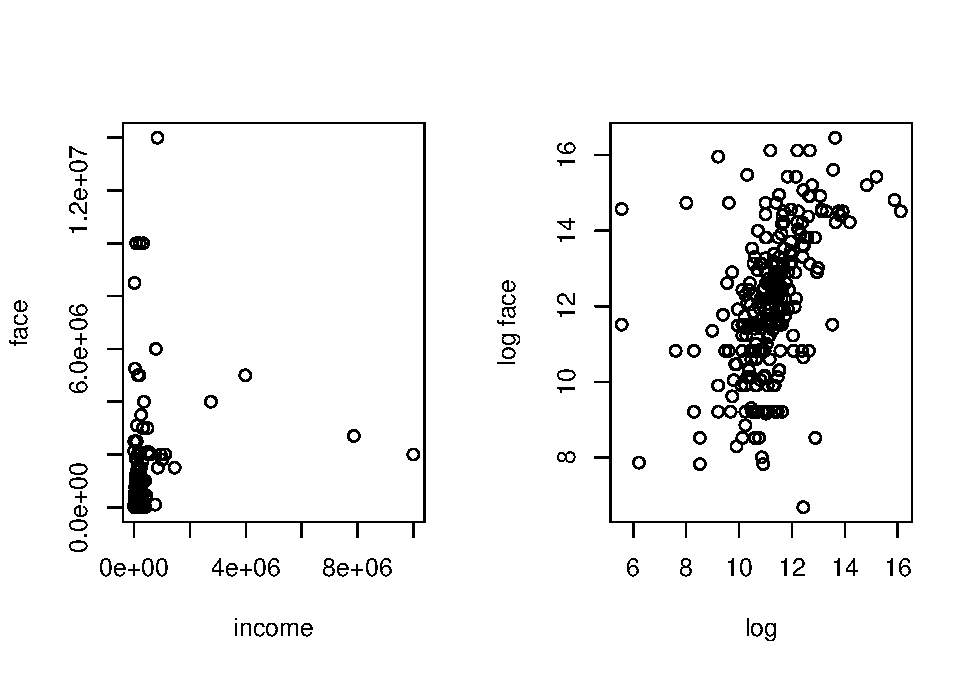
\includegraphics{RegressModelDataCamp_files/figure-latex/unnamed-chunk-91-1.pdf}

\section{Method of least squares}\label{method-of-least-squares-1}

\begin{center}\rule{0.5\linewidth}{\linethickness}\end{center}

In this section, you learn how to:

\begin{itemize}
\tightlist
\item
  Interpret correlation coefficients by visualizing a scatterplot matrix
\item
  Fit a plane to data using the method of least squares
\item
  Predict an observation using a least squares fitted plane
\end{itemize}

\begin{center}\rule{0.5\linewidth}{\linethickness}\end{center}

\subsection{Video}\label{video-9}

\subsubsection*{Video Overhead Details}\label{video-overhead-details-9}
\addcontentsline{toc}{subsubsection}{Video Overhead Details}

Show Overhead A Details. Correlation table

\hypertarget{toggleOver3.1A}{}
\begin{Shaded}
\begin{Highlighting}[]
\KeywordTok{round}\NormalTok{(}\KeywordTok{cor}\NormalTok{(Term2), }\DataTypeTok{digits=}\DecValTok{3}\NormalTok{)}
\end{Highlighting}
\end{Shaded}

\begin{verbatim}
          education  face income logface logincome  numhh
education     1.000 0.244  0.163   0.383     0.343 -0.064
face          0.244 1.000  0.217   0.656     0.323  0.107
income        0.163 0.217  1.000   0.251     0.518  0.142
logface       0.383 0.656  0.251   1.000     0.482  0.288
logincome     0.343 0.323  0.518   0.482     1.000  0.179
numhh        -0.064 0.107  0.142   0.288     0.179  1.000
\end{verbatim}

Show Overhead B Details. Scatterplot matrix

\hypertarget{toggleOver3.1B}{}
\begin{Shaded}
\begin{Highlighting}[]
\NormalTok{Term3 <-}\StringTok{ }\NormalTok{Term1[,}\KeywordTok{c}\NormalTok{(}\StringTok{"numhh"}\NormalTok{, }\StringTok{"education"}\NormalTok{, }\StringTok{"logincome"}\NormalTok{, }\StringTok{"logface"}\NormalTok{)]}
\KeywordTok{pairs}\NormalTok{(Term3, }\DataTypeTok{upper.panel =} \OtherTok{NULL}\NormalTok{, }\DataTypeTok{gap =} \DecValTok{0}\NormalTok{, }\DataTypeTok{cex.labels =} \FloatTok{1.25}\NormalTok{)}
\end{Highlighting}
\end{Shaded}

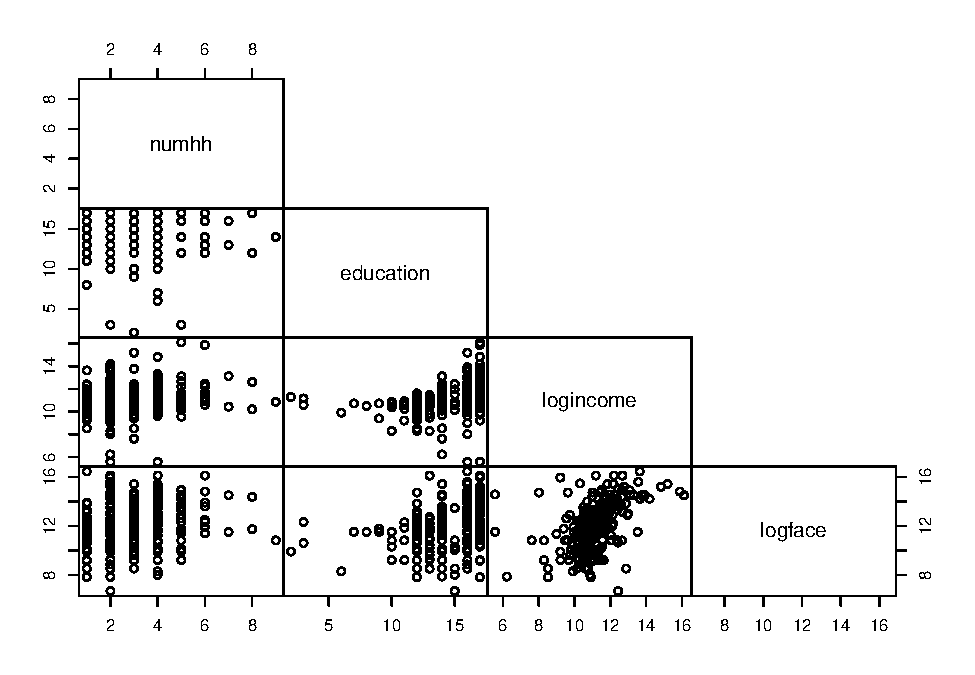
\includegraphics{RegressModelDataCamp_files/figure-latex/unnamed-chunk-93-1.pdf}

Show Overhead C Details. Visualizing a regression plane

\hypertarget{toggleOver3.1C}{}
\begin{Shaded}
\begin{Highlighting}[]
\NormalTok{education <-}\StringTok{ }\KeywordTok{seq}\NormalTok{(}\DecValTok{3}\NormalTok{, }\DecValTok{16}\NormalTok{, }\DataTypeTok{length =} \DecValTok{15}\NormalTok{)}
\NormalTok{logincome <-}\StringTok{ }\KeywordTok{seq}\NormalTok{(}\DecValTok{5}\NormalTok{, }\DecValTok{15}\NormalTok{, }\DataTypeTok{length =} \DecValTok{15}\NormalTok{)}
\NormalTok{f <-}\StringTok{ }\ControlFlowTok{function}\NormalTok{(education,logincome)\{ }
\NormalTok{  r <-}\StringTok{ }\DecValTok{5} \OperatorTok{+}\StringTok{ }\FloatTok{0.221}\OperatorTok{*}\NormalTok{education }\OperatorTok{+}\StringTok{ }\FloatTok{0.354}\OperatorTok{*}\NormalTok{logincome}
\NormalTok{\}}
\NormalTok{logface <-}\StringTok{ }\KeywordTok{outer}\NormalTok{(education, logincome, f)}
\KeywordTok{persp}\NormalTok{(education, logincome, logface, }\DataTypeTok{theta =} \DecValTok{30}\NormalTok{, }
      \DataTypeTok{phi =} \DecValTok{30}\NormalTok{, }\DataTypeTok{expand =} \FloatTok{0.5}\NormalTok{, }\DataTypeTok{ticktype =} \StringTok{"detailed"}\NormalTok{)}
\end{Highlighting}
\end{Shaded}

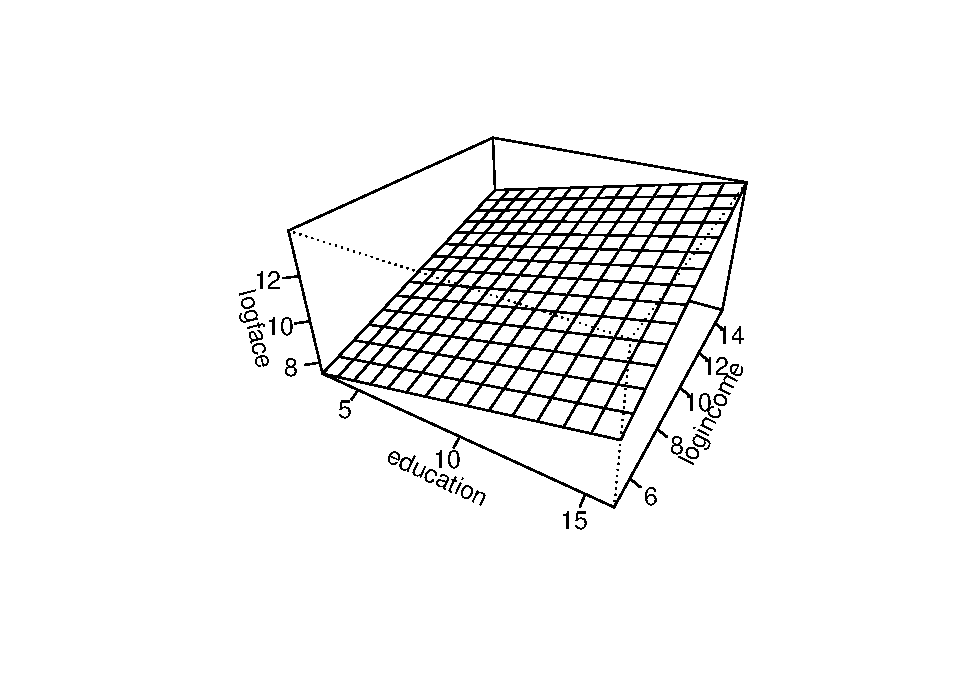
\includegraphics{RegressModelDataCamp_files/figure-latex/unnamed-chunk-94-1.pdf}

\begin{Shaded}
\begin{Highlighting}[]
\KeywordTok{rm}\NormalTok{(education,logincome,logface)}
\end{Highlighting}
\end{Shaded}

\begin{Shaded}
\begin{Highlighting}[]
\NormalTok{education <-}\StringTok{ }\KeywordTok{seq}\NormalTok{(}\DecValTok{3}\NormalTok{, }\DecValTok{16}\NormalTok{, }\DataTypeTok{length =} \DecValTok{15}\NormalTok{)}
\NormalTok{logincome <-}\StringTok{ }\KeywordTok{seq}\NormalTok{(}\DecValTok{5}\NormalTok{, }\DecValTok{15}\NormalTok{, }\DataTypeTok{length =} \DecValTok{15}\NormalTok{)}
\NormalTok{f <-}\StringTok{ }\ControlFlowTok{function}\NormalTok{(education,logincome)\{ }
\NormalTok{  r <-}\StringTok{ }\DecValTok{5} \OperatorTok{+}\StringTok{ }\FloatTok{0.221}\OperatorTok{*}\NormalTok{education }\OperatorTok{+}\StringTok{ }\FloatTok{0.354}\OperatorTok{*}\NormalTok{logincome}
\NormalTok{\}}
\NormalTok{logface <-}\StringTok{ }\KeywordTok{outer}\NormalTok{(education, logincome, f)}
\KeywordTok{persp}\NormalTok{(education, logincome, logface, }\DataTypeTok{theta =} \DecValTok{30}\NormalTok{, }
      \DataTypeTok{phi =} \DecValTok{30}\NormalTok{, }\DataTypeTok{expand =} \FloatTok{0.5}\NormalTok{, }\DataTypeTok{ticktype =} \StringTok{"simple"}\NormalTok{, }\CommentTok{#ticktype = "detailed", #}
      \DataTypeTok{xlab =} \StringTok{"x1"}\NormalTok{, }\DataTypeTok{ylab=}\StringTok{"x2"}\NormalTok{,}\DataTypeTok{zlab=}\StringTok{"y"}\NormalTok{, }\DataTypeTok{nticks =} \DecValTok{1}\NormalTok{)}
\end{Highlighting}
\end{Shaded}

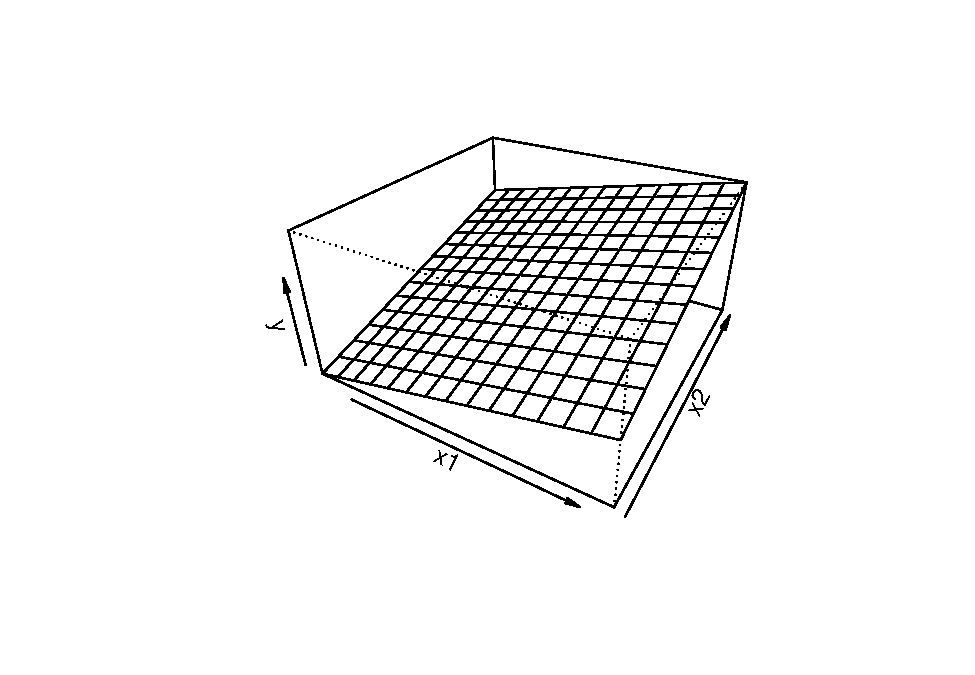
\includegraphics{RegressModelDataCamp_files/figure-latex/unnamed-chunk-95-1.pdf}

\begin{Shaded}
\begin{Highlighting}[]
\KeywordTok{rm}\NormalTok{(education,logincome,logface)}
\end{Highlighting}
\end{Shaded}

Show Overhead D Details. Method of least squares

\hypertarget{toggleOver3.1D}{}
\begin{itemize}
\tightlist
\item
  For observation \(\{(y, x_1, \ldots, x_k)\}\), the height of the
  regression plane is \[b_0 + b_1 x_1 + \cdots + b_k x_k .\]
\item
  Thus, \(y - (b_0 + b_1 x_1 + \cdots + b_k x_k)\) represents the
  deviation.
\item
  The sum of squared deviations is
  \[SS(b_0, \ldots, b_k) = \sum (y - (b_0 + b_1 x_1 + \cdots + b_k x_k))^2 .\]
\item
  The \emph{method of least squares} -- determine values of
  \(b_0, \ldots, b_k\) that minimize \(SS\).
\end{itemize}

Show Overhead E Details. Fit a multiple linear regression model

\hypertarget{toggleOver3.1E}{}
\begin{Shaded}
\begin{Highlighting}[]
\NormalTok{Term_mlr <-}\StringTok{ }\KeywordTok{lm}\NormalTok{(logface }\OperatorTok{~}\StringTok{ }\NormalTok{education }\OperatorTok{+}\StringTok{ }\NormalTok{numhh }\OperatorTok{+}\StringTok{ }\NormalTok{logincome, }\DataTypeTok{data =}\NormalTok{ Term2)}
\KeywordTok{round}\NormalTok{(}\KeywordTok{coefficients}\NormalTok{(Term_mlr), }\DataTypeTok{digits=}\DecValTok{4}\NormalTok{)}
\NormalTok{newdata <-}\StringTok{ }\KeywordTok{data.frame}\NormalTok{(}\DataTypeTok{logincome =} \KeywordTok{log}\NormalTok{(}\DecValTok{60000}\NormalTok{), }\DataTypeTok{education =} \DecValTok{12}\NormalTok{, }\DataTypeTok{numhh =} \DecValTok{3}\NormalTok{)}
\KeywordTok{exp}\NormalTok{(}\KeywordTok{predict}\NormalTok{(Term_mlr, newdata))}
\end{Highlighting}
\end{Shaded}

\begin{verbatim}
(Intercept)   education       numhh   logincome 
     2.5841      0.2064      0.3060      0.4935 
       1 
90135.86 
\end{verbatim}

\subsection{Exercise. Least squares and term life
data}\label{exercise.-least-squares-and-term-life-data}

\textbf{Assignment Text}

The prior video introduced the \emph{Survey of Consumer Finances} (SCF)
term life data. A subset consisting of only those who purchased term
life insurance, has already been read into a dataframe \texttt{Term2}.

Suppose that you wish to predict the amount of term life insurance that
someone will purchase but are uneasy about the \texttt{education}
variable. The SCF \texttt{education} variable is the number of completed
years of schooling and so 12 corresponds to completing high school in
the US. Your sense is that, for purposes of purchasing life insurance,
high school graduates and those that attend college should be treated
the same. So, in this exercise, your will create a new variable,
\texttt{education1}, that is equal to years of education for those with
education less than or equal to 12 and is equal to 12 otherwise.

\textbf{Instructions}

\begin{itemize}
\tightlist
\item
  Use the
  \href{https://www.rdocumentation.org/packages/mc2d/versions/0.1-17/topics/pmin}{pmin()}
  function to create the \texttt{education1} variable as part of the
  \texttt{Term2} dataframe.
\item
  Check your work by examining summary statistics for the revised
  \texttt{Term2} dataframe.
\item
  Examine correlations for the revised dataframe.
\item
  Using the method of least squares and the function
  \href{https://www.rdocumentation.org/packages/stats/versions/3.5.0/topics/lm}{lm()},
  fit a MLR model using \texttt{logface} as the dependent variables and
  using \texttt{education}, \texttt{numhh}, and \texttt{logincome} as
  explanatory variables.
\item
  With this fitted model and the function
  \href{https://www.rdocumentation.org/packages/stats/versions/3.5.0/topics/predict}{predict()},
  predict the face amount of insurance that someone with income of
  40,000, 11 years of education, and 4 people in the household would
  purchase.
\end{itemize}

\textbf{Hint.} Remember that your prediction is in log dollars so you
need to exponentiate it to get the results in the original dollar units

eyJsYW5ndWFnZSI6InIiLCJwcmVfZXhlcmNpc2VfY29kZSI6IiNUZXJtIDwtIHJlYWQuY3N2KFwiQ1NWRGF0YVxcXFx0ZXJtX2xpZmUuY3N2XCIsIGhlYWRlciA9IFRSVUUpXG5UZXJtIDwtIHJlYWQuY3N2KFwiaHR0cHM6Ly9hc3NldHMuZGF0YWNhbXAuY29tL3Byb2R1Y3Rpb24vcmVwb3NpdG9yaWVzLzI2MTAvZGF0YXNldHMvZWZjNjRiYzJkNzhjZjZiNDhhZDJjM2Y1ZTMxODAwY2I3NzNkZTI2MS90ZXJtX2xpZmUuY3N2XCIsIGhlYWRlciA9IFRSVUUpXG5UZXJtMSA8LSBzdWJzZXQoVGVybSwgc3Vic2V0ID0gZmFjZSA+IDApXG5UZXJtMiA8LSBUZXJtMVssIGMoXCJlZHVjYXRpb25cIiwgXCJmYWNlXCIsIFwiaW5jb21lXCIsIFwibG9nZmFjZVwiLCBcImxvZ2luY29tZVwiLCBcIm51bWhoXCIpXSIsInNhbXBsZSI6IiMgQ3JlYXRlIHRoZSBgZWR1Y2F0aW9uMWAgdmFyaWFibGUgYXMgcGFydCBvZiB0aGUgYFRlcm0yYCBkYXRhZnJhbWUuXG5UZXJtMiRlZHVjYXRpb24xIDwtIHBtaW4oMTIsIFRlcm0yJGVkdWNhdGlvbilcblxuIyBDaGVjayB5b3VyIHdvcmsgYnkgZXhhbWluaW5nIHN1bW1hcnkgc3RhdGlzdGljcyBmb3IgdGhlIHJldmlzZWQgYFRlcm0yYCBkYXRhZnJhbWUuXG5zdW1tYXJ5KF9fXylcblxuIyBFeGFtaW5lIGNvcnJlbGF0aW9ucyBmb3IgdGhlIHJldmlzZWQgZGF0YWZyYW1lLlxucm91bmQoY29yKF9fXyksIGRpZ2l0cz0zKVxuXG4jIEZpdCBhIE1MUiBtb2RlbCB1c2luZyBgbG9nZmFjZWAgYXMgdGhlIGRlcGVuZGVudCB2YXJpYWJsZXMgYW5kIHVzaW5nIGBlZHVjYXRpb25gLCBgbnVtaGhgLCBhbmQgYGxvZ2luY29tZWAgYXMgZXhwbGFuYXRvcnkgdmFyaWFibGVzLlxuVGVybV9tbHIyIDwtIGxtKGxvZ2ZhY2UgfiBfX18gKyBudW1oaCArIGxvZ2luY29tZSwgZGF0YSA9IFRlcm0yKVxuXG4jIFByZWRpY3QgdGhlIGZhY2UgYW1vdW50IG9mIGluc3VyYW5jZSB0aGF0IHNvbWVvbmUgd2l0aCBpbmNvbWUgb2YgNDAsMDAwLCAxMSB5ZWFycyBvZiBlZHVjYXRpb24sIGFuZCA0IHBlb3BsZSBpbiB0aGUgaG91c2Vob2xkIHdvdWxkIHB1cmNoYXNlLlxubmV3ZGF0YSA8LSBkYXRhLmZyYW1lKGxvZ2luY29tZSA9IGxvZyg0MDAwMCksIGVkdWNhdGlvbjEgPSAxMSwgbnVtaGggPSA0KVxuZXhwKHByZWRpY3QoX19fLCBuZXdkYXRhKSkiLCJzb2x1dGlvbiI6IlRlcm0yJGVkdWNhdGlvbjEgPC0gcG1pbigxMiwgVGVybTIkZWR1Y2F0aW9uKVxuc3VtbWFyeShUZXJtMilcbnJvdW5kKGNvcihUZXJtMiksIGRpZ2l0cz0zKVxuVGVybV9tbHIyIDwtIGxtKGxvZ2ZhY2UgfiBlZHVjYXRpb24xICsgbnVtaGggKyBsb2dpbmNvbWUsIGRhdGEgPSBUZXJtMilcbm5ld2RhdGEgPC0gZGF0YS5mcmFtZShsb2dpbmNvbWUgPSBsb2coNDAwMDApLCBlZHVjYXRpb24xID0gMTEsIG51bWhoID0gNClcbmV4cChwcmVkaWN0KFRlcm1fbWxyMiwgbmV3ZGF0YSkpIiwic2N0IjoiZXgoKSAlPiUgY2hlY2tfb2JqZWN0KFwiVGVybTJcIikgJT4lIGNoZWNrX2NvbHVtbihcImVkdWNhdGlvbjFcIikgJT4lIGNoZWNrX2VxdWFsKClcbmV4KCkgJT4lIGNoZWNrX2Z1bmN0aW9uKFwic3VtbWFyeVwiKSAlPiUge1xuICBjaGVja19hcmcoLiwgXCJvYmplY3RcIikgJT4lIGNoZWNrX2VxdWFsKClcbiAgY2hlY2tfcmVzdWx0KCkgJT4lIGNoZWNrX2VxdWFsKClcbn1cbmV4KCkgJT4lIGNoZWNrX2Z1bmN0aW9uKFwicm91bmRcIikgJT4lIHtcbiAgY2hlY2tfYXJnKC4sIFwieFwiKSAlPiUgY2hlY2tfZXF1YWwoKVxuICBjaGVja19hcmcoLiwgXCJkaWdpdHNcIikgJT4lIGNoZWNrX2VxdWFsKClcbn1cbmV4KCkgJT4lIGNoZWNrX29iamVjdChcIlRlcm1fbWxyMlwiKSAlPiUgY2hlY2tfZXF1YWwoKVxuZXgoKSAlPiUgY2hlY2tfZnVuY3Rpb24oXCJsbVwiKSAlPiUge1xuICBjaGVja19hcmcoLiwgXCJmb3JtdWxhXCIpICU+JSBjaGVja19lcXVhbCgpXG4gIGNoZWNrX2FyZyguLCBcImRhdGFcIikgJT4lIGNoZWNrX2VxdWFsKClcbn1cbmV4KCkgJT4lIGNoZWNrX29iamVjdChcIm5ld2RhdGFcIikgJT4lIGNoZWNrX2VxdWFsKClcbmV4KCkgJT4lIGNoZWNrX2Z1bmN0aW9uKFwiZXhwXCIpICU+JSBjaGVja19yZXN1bHQoKSAlPiUgY2hlY2tfZXF1YWwoKVxuZXgoKSAlPiUgY2hlY2tfZnVuY3Rpb24oXCJwcmVkaWN0XCIpICU+JSB7XG4gIGNoZWNrX2FyZyguLCBcIm9iamVjdFwiKSAlPiUgY2hlY2tfZXF1YWwoKVxuICBjaGVja19hcmcoLiwgXCJuZXdkYXRhXCIpICU+JSBjaGVja19lcXVhbCgpXG59XG5zdWNjZXNzX21zZyhcIkNvbmdyYXR1bGF0aW9ucyEgWW91IG5vdyBoYXZlIGV4cGVyaWVuY2UgZml0dGluZyBhIHJlZ3Jlc3Npb24gcGxhbmUgYW5kIHVzaW5nIHRoaXMgcGxhbmUgZm9yIHByZWRpY3Rpb25zLiBQcmVkaWN0aW9uIGlzIG9uZSBvZiB0aGUga2V5IHRhc2tzIG9mICdwcmVkaWN0aXZlIG1vZGVsaW5nLicgV2VsbCBkb25lIVwiKSJ9

\subsection{Exercise. Interpreting coefficients as proportional
changes}\label{exercise.-interpreting-coefficients-as-proportional-changes}

\textbf{Assignment Text}

In a previous exercise, you fit a MLR model using \texttt{logface} as
the outcome variable and using \texttt{education}, \texttt{numhh}, and
\texttt{logincome} as explanatory variables; the resulting fit is in the
object \texttt{Term\_mlr}. For this fit, the coefficient associated with
\texttt{education} is 0.2064. We now wish to interpret this regression
coefficient.

The typical interpretation of coefficients in a regression model is as a
partial slope. That is, for the coefficient \(b_1\) associated with
\(x_1\), we interpret \(b_1\) to be amount that the expected outcome
changes per unit change in \(x_1\), holding the other explanatory
variables fixed.

For the term life example, the units of the outcome are in logarithmic
dollars. So, for small values of \(b_1\), we can interpret this to be a
\emph{proportional} change in dollars.

\textbf{Instructions}

\begin{itemize}
\tightlist
\item
  Determine least square fitted values for several selected values of
  \texttt{education}, holding other explantory variables fixed. For this
  part of the demonstration, we used their mean values.
\item
  Determine the proportional changes. Note the relation between these
  values from a discrete change approximation to the regression
  coefficient for \texttt{education} equal to 0.2064.
\end{itemize}

eyJsYW5ndWFnZSI6InIiLCJwcmVfZXhlcmNpc2VfY29kZSI6IiNUZXJtIDwtIHJlYWQuY3N2KFwiQ1NWRGF0YVxcXFx0ZXJtX2xpZmUuY3N2XCIsIGhlYWRlciA9IFRSVUUpXG5UZXJtIDwtIHJlYWQuY3N2KFwiaHR0cHM6Ly9hc3NldHMuZGF0YWNhbXAuY29tL3Byb2R1Y3Rpb24vcmVwb3NpdG9yaWVzLzI2MTAvZGF0YXNldHMvZWZjNjRiYzJkNzhjZjZiNDhhZDJjM2Y1ZTMxODAwY2I3NzNkZTI2MS90ZXJtX2xpZmUuY3N2XCIsIGhlYWRlciA9IFRSVUUpXG5UZXJtMSA8LSBzdWJzZXQoVGVybSwgc3Vic2V0ID0gZmFjZSA+IDApXG5UZXJtMiA8LSBUZXJtMVssIGMoXCJlZHVjYXRpb25cIiwgXCJmYWNlXCIsIFwiaW5jb21lXCIsIFwibG9nZmFjZVwiLCBcImxvZ2luY29tZVwiLCBcIm51bWhoXCIpXVxuVGVybV9tbHIgPC0gbG0obG9nZmFjZSB+IGVkdWNhdGlvbiArIG51bWhoICsgbG9naW5jb21lLCBkYXRhID0gVGVybTIpIiwic2FtcGxlIjoiVGVybV9tbHIgPC0gbG0obG9nZmFjZSB+IGVkdWNhdGlvbiArIG51bWhoICsgbG9naW5jb21lLCBkYXRhID0gVGVybTIpXG5zdW1tYXJ5KFRlcm1fbWxyKSRjb2VmZmljaWVudHNbLDFdXG5cbiMgRGV0ZXJtaW5lIGxlYXN0IHNxdWFyZSBmaXR0ZWQgdmFsdWVzIGZvciBzZXZlcmFsIHNlbGVjdGVkIHZhbHVlcyBvZiBgZWR1Y2F0aW9uYCwgaG9sZGluZyBvdGhlciBleHBsYW50b3J5IHZhcmlhYmxlcyBmaXhlZC5cbmVkdWNfcHJlZGljdCA8LSBjKDE0LDE0LjEsMTQuMiwxNC4zKVxubmV3ZGF0YTEgPC0gZGF0YS5mcmFtZShsb2dpbmNvbWUgPSBtZWFuKFRlcm0yJGxvZ2luY29tZSksIGVkdWNhdGlvbiA9IGVkdWNfcHJlZGljdCwgbnVtaGggPSBtZWFuKFRlcm0yJG51bWhoKSlcbmxzZml0czEgPC0gcHJlZGljdChUZXJtX21sciwgbmV3ZGF0YTEpXG5sc2ZpdHMxXG5cbiMgRGV0ZXJtaW5lIHRoZSBwcm9wb3J0aW9uYWwgY2hhbmdlcy4gTm90ZSB0aGUgcmVsYXRpb24gYmV0d2VlbiB0aGVzZSB2YWx1ZXMgZnJvbSBhIGRpc2NyZXRlIGNoYW5nZSBhcHByb3hpbWF0aW9uIHRvIHRoZSByZWdyZXNzaW9uIGNvZWZmaWNpZW50IGZvciBgZWR1Y2F0aW9uYCBlcXVhbCB0byAwLjIwNjQuXG5sc2ZpdHMxWzI6NF0gLSBsc2ZpdHMxWzE6M11cbnBjaGFuZ2VfZml0czEgPC0gZXhwKGxzZml0czFbMjo0XSAtIGxzZml0czFbMTozXSlcbnBjaGFuZ2VfZml0czEiLCJzb2x1dGlvbiI6ImVkdWNfcHJlZGljdCA8LSBjKDE0LDE0LjEsMTQuMiwxNC4zKVxubmV3ZGF0YTEgPC0gZGF0YS5mcmFtZShsb2dpbmNvbWUgPSBtZWFuKFRlcm0yJGxvZ2luY29tZSksIGVkdWNhdGlvbiA9IGVkdWNfcHJlZGljdCwgbnVtaGggPSBtZWFuKFRlcm0yJG51bWhoKSlcbmxzZml0czEgPC0gcHJlZGljdChUZXJtX21sciwgbmV3ZGF0YTEpXG5sc2ZpdHMxXG5sc2ZpdHMxWzI6NF0gLSBsc2ZpdHMxWzE6M11cbnBjaGFuZ2VfZml0czEgPC0gZXhwKGxzZml0czFbMjo0XSAtIGxzZml0czFbMTozXSlcbnBjaGFuZ2VfZml0czEiLCJzY3QiOiJleCgpICU+JSBjaGVja19vYmplY3QoXCJlZHVjX3ByZWRpY3RcIikgJT4lIGNoZWNrX2VxdWFsKClcbmV4KCkgJT4lIGNoZWNrX29iamVjdChcIm5ld2RhdGExXCIpICU+JSBjaGVja19lcXVhbCgpXG5leCgpICU+JSBjaGVja19mdW5jdGlvbihcInByZWRpY3RcIikgJT4lIHtcbiAgY2hlY2tfYXJnKC4sIFwib2JqZWN0XCIpICU+JSBjaGVja19lcXVhbCgpXG4gIGNoZWNrX2FyZyguLCBcIm5ld2RhdGFcIikgJT4lIGNoZWNrX2VxdWFsKClcbn1cbmV4KCkgJT4lIGNoZWNrX29iamVjdChcImxzZml0czFcIikgJT4lIGNoZWNrX2VxdWFsKClcbmV4KCkgJT4lIGNoZWNrX29wZXJhdG9yKFwiLVwiLGluZGV4PTEpICU+JSBjaGVja19yZXN1bHQoKSAlPiUgY2hlY2tfZXF1YWwoKVxuZXgoKSAlPiUgY2hlY2tfb2JqZWN0KFwicGNoYW5nZV9maXRzMVwiKSAlPiUgY2hlY2tfZXF1YWwoKVxuZXgoKSAlPiUgY2hlY2tfZnVuY3Rpb24oXCJleHBcIikgJT4lIGNoZWNrX2FyZyhcInhcIikgJT4lIGNoZWNrX2VxdWFsKClcbnN1Y2Nlc3NfbXNnKFwiQ29uZ3JhdHVsYXRpb25zISBGcm9tIGNhbGN1bHVzLCBzbWFsbCBjaGFuZ2VzIGluIGxvZ2FyaXRobWljIHZhbHVlcyBjYW4gYmUgaW50ZXJwcmV0ZWQgYXMgcHJvcG9ydGlvbmFsIGNoYW5nZXMuIFRoaXMgaXMgdGhlIHJlYXNvbiBmb3IgdXNpbmcgbmF0dXJhbCBsb2dhcml0aG1zLlwiKSJ9

\subsection{Exercise. Interpreting coefficients as
elasticities}\label{exercise.-interpreting-coefficients-as-elasticities}

\textbf{Assignment Text}

In a previous exercise, you fit a MLR model using \texttt{logface} as
the outcome variable and using \texttt{education}, \texttt{numhh}, and
\texttt{logincome} as explanatory variables; the resulting fit is in the
object \texttt{Term\_mlr}. From this fit, the coefficient associated
with \texttt{logincome} is 0.4935. We now wish to interpret this
regression coefficient.

The typical interpretation of coefficients in a regression model is as a
partial slope. When both \(x_1\) and \(y\) are in logarithmic units,
then we can interpret \(b_1\) to be ratio of two percentage changes,
known as an \emph{elasticity} in economics. Mathematically, we summarize
this as \[
\frac{\partial \ln y}{\partial \ln x} = \left(\frac{\partial y}{y}\right) ~/ ~\left(\frac{\partial x}{x}\right) .
\]

\textbf{Instructions}

\begin{itemize}
\tightlist
\item
  For several selected values of \texttt{logincome}, determine the
  corresponding proportional changes.
\item
  Determine least square fitted values for several selected values of
  \texttt{logincome}, holding other explantory variables fixed.
\item
  Determine the corresponding proportional changes for the fitted
  values.
\item
  Calculate the ratio of proportional changes of fitted values to those
  for income. Note the relation between these values (from a discrete
  change approximation) to the regression coefficient for
  \texttt{logincome} equal to 0.4935.
\end{itemize}

\textbf{Hint.} When you calculate the ratio of proportional changes of
fitted values to those for income, note the relation between these
values (from a discrete change approximation) to the regression
coefficient for \texttt{logincome} equal to 0.4935.

eyJsYW5ndWFnZSI6InIiLCJwcmVfZXhlcmNpc2VfY29kZSI6IiNUZXJtIDwtIHJlYWQuY3N2KFwiQ1NWRGF0YVxcXFx0ZXJtX2xpZmUuY3N2XCIsIGhlYWRlciA9IFRSVUUpXG5UZXJtIDwtIHJlYWQuY3N2KFwiaHR0cHM6Ly9hc3NldHMuZGF0YWNhbXAuY29tL3Byb2R1Y3Rpb24vcmVwb3NpdG9yaWVzLzI2MTAvZGF0YXNldHMvZWZjNjRiYzJkNzhjZjZiNDhhZDJjM2Y1ZTMxODAwY2I3NzNkZTI2MS90ZXJtX2xpZmUuY3N2XCIsIGhlYWRlciA9IFRSVUUpXG5UZXJtMSA8LSBzdWJzZXQoVGVybSwgc3Vic2V0ID0gZmFjZSA+IDApXG5UZXJtMiA8LSBUZXJtMVssIGMoXCJlZHVjYXRpb25cIiwgXCJmYWNlXCIsIFwiaW5jb21lXCIsIFwibG9nZmFjZVwiLCBcImxvZ2luY29tZVwiLCBcIm51bWhoXCIpXVxuVGVybV9tbHIgPC0gbG0obG9nZmFjZSB+IGVkdWNhdGlvbiArIG51bWhoICsgbG9naW5jb21lLCBkYXRhID0gVGVybTIpIiwic2FtcGxlIjoiVGVybV9tbHIgPC0gbG0obG9nZmFjZSB+IGVkdWNhdGlvbiArIG51bWhoICsgbG9naW5jb21lLCBkYXRhID0gVGVybTIpXG5zdW1tYXJ5KFRlcm1fbWxyKSRjb2VmZmljaWVudHNbLDFdXG4jIEZvciBzZXZlcmFsIHNlbGVjdGVkIHZhbHVlcyBvZiBgbG9naW5jb21lYCwgZGV0ZXJtaW5lIHRoZSBjb3JyZXNwb25kaW5nIHByb3BvcnRpb25hbCBjaGFuZ2VzLlxubG9naW5jb21lX3ByZWQgPC0gYygxMSwxMS4xLDExLjIsMTEuMylcbnBjaGFuZ2VfaW5jb21lIDwtIDEwMCooZXhwKGxvZ2luY29tZV9wcmVkWzI6NF0pL2V4cChsb2dpbmNvbWVfcHJlZFsxOjNdKS0xKVxucGNoYW5nZV9pbmNvbWVcblxuIyBEZXRlcm1pbmUgbGVhc3Qgc3F1YXJlIGZpdHRlZCB2YWx1ZXMgZm9yIHNldmVyYWwgc2VsZWN0ZWQgdmFsdWVzIG9mIGBsb2dpbmNvbWVgLCBob2xkaW5nIG90aGVyIGV4cGxhbnRvcnkgdmFyaWFibGVzIGZpeGVkLlxubmV3ZGF0YTIgPC0gZGF0YS5mcmFtZShsb2dpbmNvbWUgPSBsb2dpbmNvbWVfcHJlZCwgZWR1Y2F0aW9uID0gbWVhbihUZXJtMiRlZHVjYXRpb24pLCBudW1oaCA9IG1lYW4oVGVybTIkbnVtaGgpKVxubHNmaXRzMiA8LSBwcmVkaWN0KFRlcm1fbWxyLCBuZXdkYXRhMilcblxuIyBEZXRlcm1pbmUgdGhlIGNvcnJlc3BvbmRpbmcgcHJvcG9ydGlvbmFsIGNoYW5nZXMgZm9yIHRoZSBmaXR0ZWQgdmFsdWVzLiBcbnBjaGFuZ2VfZml0czIgPC0gMTAwKihleHAobHNmaXRzMlsyOjRdKS9leHAobHNmaXRzMlsxOjNdKS0xKVxucGNoYW5nZV9maXRzMlxuXG4jIENhbGN1bGF0ZSB0aGUgcmF0aW8gb2YgcHJvcG9ydGlvbmFsIGNoYW5nZXMgb2YgZml0dGVkIHZhbHVlcyB0byB0aG9zZSBmb3IgaW5jb21lLlxucGNoYW5nZV9maXRzMi9wY2hhbmdlX2luY29tZSIsInNvbHV0aW9uIjoibG9naW5jb21lX3ByZWQgPC0gYygxMSwxMS4xLDExLjIsMTEuMylcbnBjaGFuZ2VfaW5jb21lIDwtIDEwMCooZXhwKGxvZ2luY29tZV9wcmVkWzI6NF0pL2V4cChsb2dpbmNvbWVfcHJlZFsxOjNdKS0xKVxucGNoYW5nZV9pbmNvbWVcbm5ld2RhdGEyIDwtIGRhdGEuZnJhbWUobG9naW5jb21lID0gbG9naW5jb21lX3ByZWQsIGVkdWNhdGlvbiA9IG1lYW4oVGVybTIkZWR1Y2F0aW9uKSwgbnVtaGggPSBtZWFuKFRlcm0yJG51bWhoKSlcbmxzZml0czIgPC0gcHJlZGljdChUZXJtX21sciwgbmV3ZGF0YTIpXG5wY2hhbmdlX2ZpdHMyIDwtIDEwMCooZXhwKGxzZml0czJbMjo0XSkvZXhwKGxzZml0czJbMTozXSktMSlcbnBjaGFuZ2VfZml0czJcbnBjaGFuZ2VfZml0czIvcGNoYW5nZV9pbmNvbWUiLCJzY3QiOiJleCgpICU+JSBjaGVja19vYmplY3QoXCJsb2dpbmNvbWVfcHJlZFwiKSAlPiUgY2hlY2tfZXF1YWwoKVxuZXgoKSAlPiUgY2hlY2tfb2JqZWN0KFwicGNoYW5nZV9pbmNvbWVcIikgJT4lIGNoZWNrX2VxdWFsKClcbmV4KCkgJT4lIGNoZWNrX29iamVjdChcIm5ld2RhdGEyXCIpICU+JSBjaGVja19lcXVhbCgpXG5leCgpICU+JSBjaGVja19vYmplY3QoXCJsc2ZpdHMyXCIpICU+JSBjaGVjX2VxdWFsKClcbmV4KCkgJT4lIGNoZWNrX2Z1bmN0aW9uKFwicHJlZGljdFwiKSAlPiUge1xuICBjaGVja19hcmcoLiwgXCJvYmplY3RcIikgJT4lIGNoZWNrX2VxdWFsKClcbiAgY2hlY2tfYXJnKC4sIFwibmV3ZGF0YVwiKSAlPiUgY2hlY2tfZXF1YWwoKVxufVxuZXgoKSAlPiUgY2hlY2tfb2JqZWN0KFwicGNoYW5nZV9maXRzMlwiKSAlPiUgY2hlY2tfZXF1YWwoKVxuZXgoKSAlPiUgY2hlY2tfZXhwcmVzc2lvbihcIi9cIixpbmRleD0zKSAlPiUgY2hlY2tfcmVzdWx0KCkgJT4lIGNoZWNrX2VxdWFsKClcbnN1Y2Nlc3NfbXNnKFwiQ29uZ3JhdHVsYXRpb25zISBXaGVuIGJvdGggJHhfMSQgYW5kICR5JCBhcmUgaW4gbG9nYXJpdGhtaWMgdW5pdHMsIHRoZW4gd2UgY2FuIGludGVycHJldCAkYl8xJCB0byBiZSByYXRpbyBvZiB0d28gcGVyY2VudGFnZSBjaGFuZ2VzLCBrbm93biBhcyBhbiAqZWxhc3RpY2l0eSogaW4gZWNvbm9taWNzLlwiKSJ9

\section{Statistical inference and multiple linear
regresson}\label{statistical-inference-and-multiple-linear-regresson}

\begin{center}\rule{0.5\linewidth}{\linethickness}\end{center}

In this section, you learn how to:

\begin{itemize}
\tightlist
\item
  Explain mean square error and residual standard error in terms of
  degrees of freedom
\item
  Develop an ANOVA table and use it to derive the coefficient of
  determination
\item
  Calculate and interpret the coefficient of determination adjusted for
  degrees of freedom
\item
  Conduct a test of a regression coefficient
\item
  Summarize regression coefficients using point and interval estimators
\end{itemize}

\begin{center}\rule{0.5\linewidth}{\linethickness}\end{center}

\subsection{Video}\label{video-10}

\subsubsection*{Video Overhead Details}\label{video-overhead-details-10}
\addcontentsline{toc}{subsubsection}{Video Overhead Details}

Show Overhead A Details. Goodness of fit

\hypertarget{toggleOver3.2A}{}
Summarize

\begin{itemize}
\tightlist
\item
  deviations
\item
  \(s^2\)
\item
  \(R^2\)
\item
  \(R_a^2\)
\item
  ANOVA table
\end{itemize}

Show Overhead B Details. Goodness of fit and term life

\hypertarget{toggleOver3.2B}{}
\begin{Shaded}
\begin{Highlighting}[]
\NormalTok{Term_mlr <-}\StringTok{ }\KeywordTok{lm}\NormalTok{(logface }\OperatorTok{~}\StringTok{ }\NormalTok{education }\OperatorTok{+}\StringTok{ }\NormalTok{numhh }\OperatorTok{+}\StringTok{ }\NormalTok{logincome, }\DataTypeTok{data =}\NormalTok{ Term2)}
\KeywordTok{summary}\NormalTok{(Term_mlr)}
\KeywordTok{anova}\NormalTok{(Term_mlr)}
\end{Highlighting}
\end{Shaded}

\begin{verbatim}

Call:
lm(formula = logface ~ education + numhh + logincome, data = Term2)

Residuals:
    Min      1Q  Median      3Q     Max 
-5.7420 -0.8681  0.0549  0.9093  4.7187 

Coefficients:
            Estimate Std. Error t value Pr(>|t|)    
(Intercept)  2.58408    0.84643   3.053  0.00249 ** 
education    0.20641    0.03883   5.316 2.22e-07 ***
numhh        0.30605    0.06333   4.833 2.26e-06 ***
logincome    0.49353    0.07754   6.365 8.32e-10 ***
---
Signif. codes:  0 '***' 0.001 '**' 0.01 '*' 0.05 '.' 0.1 ' ' 1

Residual standard error: 1.525 on 271 degrees of freedom
Multiple R-squared:  0.3425,    Adjusted R-squared:  0.3353 
F-statistic: 47.07 on 3 and 271 DF,  p-value: < 2.2e-16

Analysis of Variance Table

Response: logface
           Df Sum Sq Mean Sq F value    Pr(>F)    
education   1 140.55 140.549  60.417 1.601e-13 ***
numhh       1  93.68  93.681  40.270 9.251e-10 ***
logincome   1  94.24  94.238  40.510 8.316e-10 ***
Residuals 271 630.43   2.326                      
---
Signif. codes:  0 '***' 0.001 '**' 0.01 '*' 0.05 '.' 0.1 ' ' 1
\end{verbatim}

Show Overhead C Details. Statistical inference

\hypertarget{toggleOver3.2C}{}
\begin{itemize}
\tightlist
\item
  hypothesis testing of a regression coefficient
\item
  confidence intervals
\end{itemize}

Show Overhead D Details. Statistical inference and term life

\hypertarget{toggleOver3.2D}{}
\begin{Shaded}
\begin{Highlighting}[]
\NormalTok{Term_mlr <-}\StringTok{ }\KeywordTok{lm}\NormalTok{(logface }\OperatorTok{~}\StringTok{ }\NormalTok{education }\OperatorTok{+}\StringTok{ }\NormalTok{numhh }\OperatorTok{+}\StringTok{ }\NormalTok{logincome, }\DataTypeTok{data =}\NormalTok{ Term2)}
\NormalTok{model_sum <-}\StringTok{ }\KeywordTok{summary}\NormalTok{(Term_mlr)}
\NormalTok{model_sum}\OperatorTok{$}\NormalTok{coefficients}

\KeywordTok{round}\NormalTok{(}\KeywordTok{confint}\NormalTok{(Term_mlr, }\DataTypeTok{level =}\NormalTok{ .}\DecValTok{95}\NormalTok{), }\DataTypeTok{digits =} \DecValTok{3}\NormalTok{)}

\KeywordTok{round}\NormalTok{(}\KeywordTok{confint}\NormalTok{(Term_mlr, }\DataTypeTok{level =}\NormalTok{ .}\DecValTok{95}\NormalTok{), }\DataTypeTok{digits =} \DecValTok{3}\NormalTok{)}
\end{Highlighting}
\end{Shaded}

\begin{verbatim}
             Estimate Std. Error  t value     Pr(>|t|)
(Intercept) 2.5840786 0.84642972 3.052916 2.491588e-03
education   0.2064139 0.03883186 5.315581 2.223619e-07
numhh       0.3060455 0.06332511 4.832926 2.255708e-06
logincome   0.4935323 0.07754198 6.364711 8.316097e-10
            2.5 % 97.5 %
(Intercept) 0.918  4.250
education   0.130  0.283
numhh       0.181  0.431
logincome   0.341  0.646
            2.5 % 97.5 %
(Intercept) 0.918  4.250
education   0.130  0.283
numhh       0.181  0.431
logincome   0.341  0.646
\end{verbatim}

\subsection{Exercise. Statistical inference and term
life}\label{exercise.-statistical-inference-and-term-life}

\textbf{Assignment Text}

In later chapters, we will learn how to specify a model using
diagnostics techniques; these techniques were used to specify face in
log dollars for the outcome and similarly income in log dollars as an
explanatory variable. Just to see how things work, in this exercise we
will create new variables \texttt{face} and \texttt{income} that are in
the original units and run a regression with these. We have already seen
that rescaling by constants do not affect relationships but can be
helpful with interpretations, so we define both \texttt{face} and
\texttt{income} to be in thousands of dollars. A prior video introduced
the term life dataframe \texttt{Term2}.

\textbf{Instructions}

\begin{itemize}
\tightlist
\item
  Create \texttt{Term2\$face} by exponentiating \texttt{logface} and
  dividing by 1000. For convenience, we are storing this variable in the
  data set \texttt{Term2}. Use the same process to create
  \texttt{Term2\$income}.
\item
  Run a regression using \texttt{face} as the outcome variable and
  \texttt{education}, \texttt{numhh}, and \texttt{income} as explanatory
  variables.
\item
  Summarize this model and identify the residual standard error (\(s\))
  as well as the coefficient of determination (\(R^2\)) and the version
  adjusted for degrees of freedom (\(R_a^2\)).
\end{itemize}

eyJsYW5ndWFnZSI6InIiLCJwcmVfZXhlcmNpc2VfY29kZSI6IiNUZXJtIDwtIHJlYWQuY3N2KFwiQ1NWRGF0YVxcXFx0ZXJtX2xpZmUuY3N2XCIsIGhlYWRlciA9IFRSVUUpXG5UZXJtIDwtIHJlYWQuY3N2KFwiaHR0cHM6Ly9hc3NldHMuZGF0YWNhbXAuY29tL3Byb2R1Y3Rpb24vcmVwb3NpdG9yaWVzLzI2MTAvZGF0YXNldHMvZWZjNjRiYzJkNzhjZjZiNDhhZDJjM2Y1ZTMxODAwY2I3NzNkZTI2MS90ZXJtX2xpZmUuY3N2XCIsIGhlYWRlciA9IFRSVUUpXG5UZXJtMSA8LSBzdWJzZXQoVGVybSwgc3Vic2V0ID0gZmFjZSA+IDApXG5UZXJtMiA8LSBUZXJtMVssIGMoXCJlZHVjYXRpb25cIiwgXCJmYWNlXCIsIFwiaW5jb21lXCIsIFwibG9nZmFjZVwiLCBcImxvZ2luY29tZVwiLCBcIm51bWhoXCIpXSIsInNhbXBsZSI6IiMgQ3JlYXRlIGBUZXJtMiRmYWNlYCBhbmQgIGBUZXJtMiRpbmNvbWVgXG5UZXJtMiRmYWNlIDwtIGV4cChfX18pL19fX1xuVGVybTIkaW5jb21lIDwtIGV4cChfX18pL19fX1xuXG4jIFJ1biBhIHJlZ3Jlc3Npb24gdXNpbmcgYGZhY2VgIGFzIHRoZSBvdXRjb21lIHZhcmlhYmxlIGFuZCBgZWR1Y2F0aW9uYCwgYG51bWhoYCwgYW5kIGBpbmNvbWVgIGFzIGV4cGxhbmF0b3J5IHZhcmlhYmxlcy5cblRlcm1fbWxyMSA8LSBsbShmYWNlIH4gX19fLCBkYXRhID0gVGVybTIpXG5cbiMgU3VtbWFyaXplIHRoaXMgbW9kZWxcbnN1bW1hcnkoVGVybV9tbHIxKSIsInNvbHV0aW9uIjoiVGVybTIkZmFjZSA8LSBleHAoVGVybTIkbG9nZmFjZSkvMTAwMFxuVGVybTIkaW5jb21lIDwtIGV4cChUZXJtMiRsb2dpbmNvbWUpLzEwMDBcblRlcm1fbWxyMSA8LSBsbShmYWNlIH4gZWR1Y2F0aW9uICsgbnVtaGggKyBpbmNvbWUsIGRhdGEgPSBUZXJtMilcbnN1bW1hcnkoVGVybV9tbHIxKSIsInNjdCI6ImV4KCkgJT4lIGNoZWNrX29iamVjdChcIlRlcm0yXCIpICU+JSB7XG4gIGNoZWNrX2NvbHVtbiguLCBcImZhY2VcIikgJT4lIGNoZWNrX2VxdWFsKClcbiAgY2hlY2tfY29sdW1uKC4sIFwiaW5jb21lXCIpICU+JSBjaGVja19lcXVhbCgpXG4gfVxuZXgoKSAlPiUgY2hlY2tfb2JqZWN0KFwiVGVybV9tbHIxXCIpICU+JSBjaGVja19lcXVhbCgpXG5leCgpICU+JSBjaGVja19mdW5jdGlvbihcImxtXCIpICU+JSB7XG4gIGNoZWNrX2FyZyguLCBcImZvcm11bGFcIikgJT4lIGNoZWNrX2VxdWFsKClcbiAgY2hlY2tfYXJnKC4sIFwiZGF0YVwiKSAlPiUgY2hlY2tfZXF1YWwoKVxufVxuZXgoKSAlPiUgY2hlY2tfZnVuY3Rpb24oXCJzdW1tYXJ5XCIpICU+JSBjaGVja19yZXN1bHQoKSAlPiUgY2hlY2tfZXF1YWwoKVxuc3VjY2Vzc19tc2coXCJDb25ncmF0dWxhdGlvbnMhIENvbXBhcmUgdGhlc2UgZ29vZG5lc3Mgb2YgZml0IG1lYXN1cmVzIHRvIHRob3NlIHdoZXJlIGluY29tZSBhbmQgZmFjZSBhcmUgaW4gbG9nYXJpdGhtaWMgdW5pdHMuIEFsdGhvdWdoIG5vdCB0aGUgb25seSBpbmRpY2F0b3JzLCB5b3Ugd2lsbCBzZWUgdGhhdCB0aGUgcHJvcG9ydGlvbiBvZiB2YXJpYWJpbGl0eSBleHBsYWluZWQgKFIgc3F1YXJlKSBhbmQgdGhlIHN0YXRpc3RpY2FsIHNpZ25pZmljYW5jZSBvZiBjb2VmZmljaWVudHMgYXJlIHN0cmlraW5nbHkgaGlnaGVyIGluIHRoZSBtb2RlbCB3aXRoIHZhcmlhYmxlcyBpbiBsb2dnZWQgdW5pdHMuXCIpIn0=

\section{Binary variables}\label{binary-variables}

\begin{center}\rule{0.5\linewidth}{\linethickness}\end{center}

In this section, you learn how to:

\begin{itemize}
\tightlist
\item
  Interpret regression coefficients associated with binary variables
\item
  Use binary variables and interaction terms to create regression models
  that are nonlinear in the covariates
\end{itemize}

\begin{center}\rule{0.5\linewidth}{\linethickness}\end{center}

\subsection{Video}\label{video-11}

\subsubsection*{Video Overhead Details}\label{video-overhead-details-11}
\addcontentsline{toc}{subsubsection}{Video Overhead Details}

Show Overhead A Details. Binary variables

\hypertarget{toggleOver3.3A}{}
\begin{itemize}
\item
  We can define a new variable \[
  single= \left\{ \begin{array}{ll}
      0 & \text{for other respondents} \\
      1 & \text{for single respondents}
  \end{array} \right.
  \]
\item
  The variable \emph{single} is said to be an \emph{indicator}, or
  \emph{dummy}, variable.
\item
  To interpret coefficients, we now consider the regression function
\end{itemize}

\[
\text{E }logface = \beta_0 + \beta_1 logincome + \beta_2 single
\] - This can be expressed as two lines \[
\text{E }logface = \left\{ \begin{array}{ll}
        \beta_0 + \beta_1  logincome           & \textrm{for other respondents} \\
        \beta_0 + \beta_2 + \beta_1  logincome & \textrm{for single respondents}
\end{array} \right. .
\] - The least squares method of calculating the estimators, and the
resulting theoretical properties, are the still valid when using binary
variables.

Show Overhead B Details. Visualize effect of binary variables

\hypertarget{toggleOver3.3B}{}

Show Overhead C Details. R script for visualization

\hypertarget{toggleOver3.3C}{}
\begin{Shaded}
\begin{Highlighting}[]
\NormalTok{Term4 <-}\StringTok{ }\NormalTok{Term1[,}\KeywordTok{c}\NormalTok{(}\StringTok{"numhh"}\NormalTok{, }\StringTok{"education"}\NormalTok{, }\StringTok{"logincome"}\NormalTok{, }\StringTok{"logface"}\NormalTok{, }\StringTok{"marstat"}\NormalTok{)]}
\NormalTok{Term4}\OperatorTok{$}\NormalTok{marstat <-}\StringTok{ }\KeywordTok{as.factor}\NormalTok{(Term4}\OperatorTok{$}\NormalTok{marstat)}
\KeywordTok{table}\NormalTok{(Term4}\OperatorTok{$}\NormalTok{marstat)}
\NormalTok{Term4}\OperatorTok{$}\NormalTok{single <-}\StringTok{ }\DecValTok{1}\OperatorTok{*}\NormalTok{(Term4}\OperatorTok{$}\NormalTok{marstat }\OperatorTok{==}\StringTok{ }\DecValTok{0}\NormalTok{)}
\NormalTok{model_single <-}\StringTok{ }\KeywordTok{lm}\NormalTok{(logface }\OperatorTok{~}\StringTok{ }\NormalTok{logincome }\OperatorTok{+}\StringTok{ }\NormalTok{single, }\DataTypeTok{data =}\NormalTok{ Term4)}
\KeywordTok{summary}\NormalTok{(model_single)}

\KeywordTok{plot}\NormalTok{(Term4}\OperatorTok{$}\NormalTok{logincome,Term4}\OperatorTok{$}\NormalTok{logface,}\DataTypeTok{xlab=}\StringTok{"logarithmic income"}\NormalTok{, }\DataTypeTok{ylab=}\StringTok{"log face"}\NormalTok{,}
    \DataTypeTok{pch=} \DecValTok{1}\OperatorTok{+}\DecValTok{16}\OperatorTok{*}\NormalTok{Term4}\OperatorTok{$}\NormalTok{single, }\DataTypeTok{col =} \KeywordTok{c}\NormalTok{(}\StringTok{"red"}\NormalTok{, }\StringTok{"black"}\NormalTok{, }\StringTok{"black"}\NormalTok{)[Term4}\OperatorTok{$}\NormalTok{marstat])}
\NormalTok{Ey1 <-}\StringTok{ }\NormalTok{model_single}\OperatorTok{$}\NormalTok{coefficients[}\DecValTok{1}\NormalTok{]}\OperatorTok{+}\NormalTok{model_single}\OperatorTok{$}\NormalTok{coefficients[}\DecValTok{2}\NormalTok{]}\OperatorTok{*}\NormalTok{Term4}\OperatorTok{$}\NormalTok{logincome}
\NormalTok{Ey2 <-}\StringTok{ }\NormalTok{Ey1 }\OperatorTok{+}\StringTok{ }\NormalTok{model_single}\OperatorTok{$}\NormalTok{coefficients[}\DecValTok{3}\NormalTok{]}
\KeywordTok{lines}\NormalTok{(Term4}\OperatorTok{$}\NormalTok{logincome, Ey1)}
\KeywordTok{lines}\NormalTok{(Term4}\OperatorTok{$}\NormalTok{logincome, Ey2, }\DataTypeTok{col=}\StringTok{"red"}\NormalTok{)}
\end{Highlighting}
\end{Shaded}

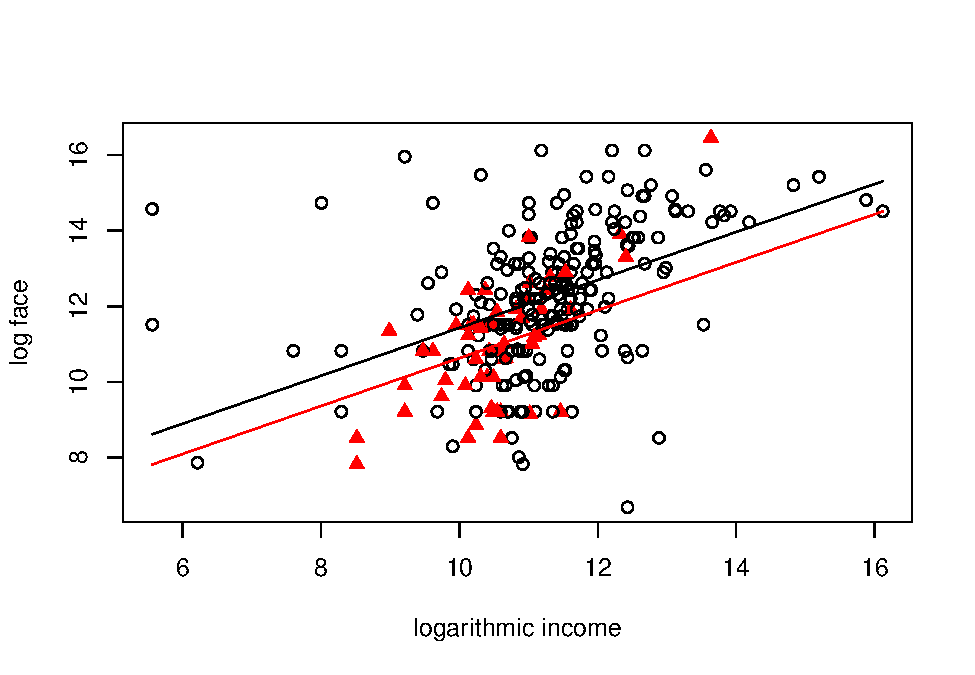
\includegraphics{RegressModelDataCamp_files/figure-latex/unnamed-chunk-115-1.pdf}

\begin{verbatim}

  0   1   2 
 57 208  10 

Call:
lm(formula = logface ~ logincome + single, data = Term4)

Residuals:
    Min      1Q  Median      3Q     Max 
-6.2828 -0.8785  0.0364  0.9227  5.9573 

Coefficients:
            Estimate Std. Error t value Pr(>|t|)    
(Intercept)  5.09007    0.88643   5.742 2.49e-08 ***
logincome    0.63378    0.07776   8.151 1.33e-14 ***
single      -0.80006    0.24796  -3.227  0.00141 ** 
---
Signif. codes:  0 '***' 0.001 '**' 0.01 '*' 0.05 '.' 0.1 ' ' 1

Residual standard error: 1.615 on 272 degrees of freedom
Multiple R-squared:  0.2605,    Adjusted R-squared:  0.255 
F-statistic:  47.9 on 2 and 272 DF,  p-value: < 2.2e-16
\end{verbatim}

Show Overhead D Details. Interaction Terms

\hypertarget{toggleOver3.3D}{}
\begin{itemize}
\tightlist
\item
  Linear regression models are defined in terms of linear combinations
  of explanatory varibles but we can expand their scope through
  nonlinear transformations
\item
  One type of nonlinear transform is the product of two varibles that is
  used to create what is known as an \emph{interaction} variable
\item
  To interpret coefficients, we now consider the regression function
\end{itemize}

\[
\text{E }logface = \beta_0 + \beta_1 logincome + \beta_2 single + \beta_3 single*logincome
\] - This can be expressed as two lines with different slopes \[
\text{E }logface = \left\{ \begin{array}{ll}
        \beta_0 + \beta_1   logincome           & \textrm{for other respondents} \\
        \beta_0 + \beta_2 + (\beta_1  + \beta_3) logincome & \textrm{for single respondents}
\end{array} \right. .
\]

Show Overhead E Details. Visualizing binary variables with interactions
terms

\hypertarget{toggleOver3.3E}{}
\begin{Shaded}
\begin{Highlighting}[]
\NormalTok{Term4 <-}\StringTok{ }\NormalTok{Term1[,}\KeywordTok{c}\NormalTok{(}\StringTok{"numhh"}\NormalTok{, }\StringTok{"education"}\NormalTok{, }\StringTok{"logincome"}\NormalTok{, }\StringTok{"logface"}\NormalTok{, }\StringTok{"marstat"}\NormalTok{)]}
\NormalTok{Term4}\OperatorTok{$}\NormalTok{marstat <-}\StringTok{ }\KeywordTok{as.factor}\NormalTok{(Term4}\OperatorTok{$}\NormalTok{marstat)}
\KeywordTok{table}\NormalTok{(Term4}\OperatorTok{$}\NormalTok{marstat)}
\NormalTok{Term4}\OperatorTok{$}\NormalTok{single <-}\StringTok{ }\DecValTok{1}\OperatorTok{*}\NormalTok{(Term4}\OperatorTok{$}\NormalTok{marstat }\OperatorTok{==}\StringTok{ }\DecValTok{0}\NormalTok{)}
\NormalTok{model_single_inter <-}\StringTok{ }\KeywordTok{lm}\NormalTok{(logface }\OperatorTok{~}\StringTok{ }\NormalTok{logincome }\OperatorTok{+}\StringTok{ }\NormalTok{single }\OperatorTok{+}\StringTok{ }\NormalTok{single}\OperatorTok{*}\NormalTok{logincome, }\DataTypeTok{data =}\NormalTok{ Term4)}
\KeywordTok{summary}\NormalTok{(model_single_inter)}

\KeywordTok{plot}\NormalTok{(Term4}\OperatorTok{$}\NormalTok{logincome,Term4}\OperatorTok{$}\NormalTok{logface,}\DataTypeTok{xlab=}\StringTok{"logarithmic income"}\NormalTok{, }\DataTypeTok{ylab=}\StringTok{"log face"}\NormalTok{,}
    \DataTypeTok{pch=} \DecValTok{1}\OperatorTok{+}\DecValTok{16}\OperatorTok{*}\NormalTok{Term4}\OperatorTok{$}\NormalTok{single, }\DataTypeTok{col =} \KeywordTok{c}\NormalTok{(}\StringTok{"red"}\NormalTok{, }\StringTok{"black"}\NormalTok{, }\StringTok{"black"}\NormalTok{)[Term4}\OperatorTok{$}\NormalTok{marstat])}
\NormalTok{Ey1 <-}\StringTok{ }\NormalTok{model_single_inter}\OperatorTok{$}\NormalTok{coefficients[}\DecValTok{1}\NormalTok{]}\OperatorTok{+}\NormalTok{model_single_inter}\OperatorTok{$}\NormalTok{coefficients[}\DecValTok{2}\NormalTok{]}\OperatorTok{*}\NormalTok{Term4}\OperatorTok{$}\NormalTok{logincome}
\NormalTok{Ey2 <-}\StringTok{ }\NormalTok{Ey1 }\OperatorTok{+}\StringTok{ }\NormalTok{model_single_inter}\OperatorTok{$}\NormalTok{coefficients[}\DecValTok{3}\NormalTok{]}\OperatorTok{+}\NormalTok{model_single_inter}\OperatorTok{$}\NormalTok{coefficients[}\DecValTok{4}\NormalTok{]}\OperatorTok{*}\NormalTok{Term4}\OperatorTok{$}\NormalTok{logincome}
\KeywordTok{lines}\NormalTok{(Term4}\OperatorTok{$}\NormalTok{logincome, Ey1)}
\KeywordTok{lines}\NormalTok{(Term4}\OperatorTok{$}\NormalTok{logincome, Ey2, }\DataTypeTok{col=}\StringTok{"red"}\NormalTok{)}
\end{Highlighting}
\end{Shaded}

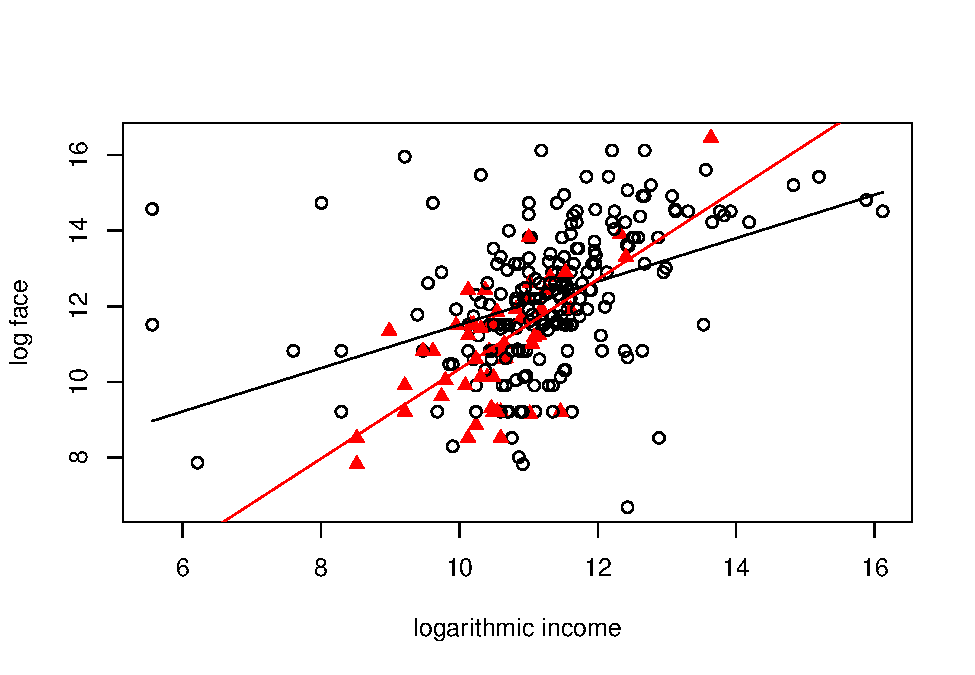
\includegraphics{RegressModelDataCamp_files/figure-latex/unnamed-chunk-116-1.pdf}

\begin{verbatim}

  0   1   2 
 57 208  10 

Call:
lm(formula = logface ~ logincome + single + single * logincome, 
    data = Term4)

Residuals:
    Min      1Q  Median      3Q     Max 
-6.2149 -0.8287  0.0696  0.9308  5.6070 

Coefficients:
                 Estimate Std. Error t value Pr(>|t|)    
(Intercept)       5.77902    0.92550   6.244 1.64e-09 ***
logincome         0.57288    0.08124   7.051 1.47e-11 ***
single           -7.29211    2.74216  -2.659   0.0083 ** 
logincome:single  0.61244    0.25764   2.377   0.0181 *  
---
Signif. codes:  0 '***' 0.001 '**' 0.01 '*' 0.05 '.' 0.1 ' ' 1

Residual standard error: 1.601 on 271 degrees of freedom
Multiple R-squared:  0.2756,    Adjusted R-squared:  0.2676 
F-statistic: 34.36 on 3 and 271 DF,  p-value: < 2.2e-16
\end{verbatim}

\subsection{Exercise. Binary variables and term
life}\label{exercise.-binary-variables-and-term-life}

\textbf{Assignment Text}

In the prior video, we saw how the variable \texttt{single} can be used
with logarithmic income to explain logarithmic face amounts of term life
insurance that people purchase. The coefficient associated with this
variable turns out to be negative which is intuitively appealing; if an
individual is single, then that person may not have the strong need to
purchase financial security for others in the event of unexpected death.

In this exercise, we will extend this by incorporating \texttt{single}
into our larger regression model that contains other explanatory
varibles, \texttt{logincome}, \texttt{education} and \texttt{numhh}. The
data have been pre-loaded into the dataframe \texttt{Term4}.

\textbf{Instructions}

\begin{itemize}
\tightlist
\item
  Calculate a table of correlation coefficients to examine pairwise
  linear relationships among the variables \texttt{numhh},
  \texttt{education}, \texttt{logincome}, \texttt{single}, and
  \texttt{logface}.
\item
  Fit a MLR model of \texttt{logface} using explanatory variables
  \texttt{numhh}, \texttt{education}, \texttt{logincome}, and
  \texttt{single}. Examine the residual standard deviation \(s\), the
  coefficient of determination \(R^2\), and the adjusted version
  \(R_a^2\). Also note the statistical significance of the coefficient
  associated with \texttt{single}.
\item
  Repeat the MLR model fit while adding the interaction term
  \texttt{single*logincome}.
\end{itemize}

eyJsYW5ndWFnZSI6InIiLCJwcmVfZXhlcmNpc2VfY29kZSI6IiNUZXJtIDwtIHJlYWQuY3N2KFwiQ1NWRGF0YVxcXFx0ZXJtX2xpZmUuY3N2XCIsIGhlYWRlciA9IFRSVUUpXG5UZXJtIDwtIHJlYWQuY3N2KFwiaHR0cHM6Ly9hc3NldHMuZGF0YWNhbXAuY29tL3Byb2R1Y3Rpb24vcmVwb3NpdG9yaWVzLzI2MTAvZGF0YXNldHMvZWZjNjRiYzJkNzhjZjZiNDhhZDJjM2Y1ZTMxODAwY2I3NzNkZTI2MS90ZXJtX2xpZmUuY3N2XCIsIGhlYWRlciA9IFRSVUUpXG5UZXJtMSA8LSBzdWJzZXQoVGVybSwgc3Vic2V0ID0gZmFjZSA+IDApXG5UZXJtNCA8LSBUZXJtMVssYyhcIm51bWhoXCIsIFwiZWR1Y2F0aW9uXCIsIFwibG9naW5jb21lXCIsIFwibWFyc3RhdFwiLCBcImxvZ2ZhY2VcIildXG5UZXJtNCRzaW5nbGUgPC0gMSooVGVybTQkbWFyc3RhdCA9PSAwKSIsInNhbXBsZSI6IiMgQ2FsY3VsYXRlIGEgdGFibGUgb2YgY29ycmVsYXRpb24gY29lZmZpY2llbnRzXG5yb3VuZChfX18oVGVybTRbLGMoXCJudW1oaFwiLCBcImVkdWNhdGlvblwiLCBcImxvZ2luY29tZVwiLCBcInNpbmdsZVwiLCBcImxvZ2ZhY2VcIildKSwgZGlnaXRzID0gMylcblxuIyBGaXQgYSBNTFIgbW9kZWwgb2YgYGxvZ2ZhY2VgIHVzaW5nIGV4cGxhbmF0b3J5IHZhcmlhYmxlcyBgbnVtaGhgLCBgZWR1Y2F0aW9uYCwgYGxvZ2luY29tZWAsIGFuZCBgc2luZ2xlYC5cblRlcm1fbWxyMyA8LSBsbShsb2dmYWNlIH4gZWR1Y2F0aW9uICsgbnVtaGggKyBsb2dpbmNvbWUgKyBzaW5nbGUsIGRhdGEgPSBUZXJtNClcbnN1bW1hcnkoVGVybV9tbHIzKVxuXG4jIFJlcGVhdCB0aGUgTUxSIG1vZGVsIGZpdCB3aGlsZSBhZGRpbmcgdGhlIGludGVyYWN0aW9uIHRlcm0gIGBzaW5nbGUqbG9naW5jb21lYC5cblRlcm1fbWxyNCA8LSBsbShsb2dmYWNlIH4gZWR1Y2F0aW9uICsgbnVtaGggKyBsb2dpbmNvbWUgKyBzaW5nbGUgKyBzaW5nbGUqbG9naW5jb21lLCBkYXRhID0gVGVybTQpXG5zdW1tYXJ5KFRlcm1fbWxyNCkiLCJzb2x1dGlvbiI6InJvdW5kKGNvcihUZXJtNFssYyhcIm51bWhoXCIsIFwiZWR1Y2F0aW9uXCIsIFwibG9naW5jb21lXCIsIFwic2luZ2xlXCIsIFwibG9nZmFjZVwiKV0pLCBkaWdpdHMgPSAzKVxuVGVybV9tbHIzIDwtIGxtKGxvZ2ZhY2UgfiBlZHVjYXRpb24gKyBudW1oaCArIGxvZ2luY29tZSArIHNpbmdsZSwgZGF0YSA9IFRlcm00KVxuc3VtbWFyeShUZXJtX21scjMpXG5UZXJtX21scjQgPC0gbG0obG9nZmFjZSB+IGVkdWNhdGlvbiArIG51bWhoICsgbG9naW5jb21lICsgc2luZ2xlICsgc2luZ2xlKmxvZ2luY29tZSwgZGF0YSA9IFRlcm00KVxuc3VtbWFyeShUZXJtX21scjQpIiwic2N0IjoiZXgoKSAlPiUgY2hlY2tfZnVuY3Rpb24oXCJyb3VuZFwiKSAlPiUgY2hlY2tfcmVzdWx0KCkgJT4lIGNoZWNrX2VxdWFsKClcbmV4KCkgJT4lIGNoZWNrX29iamVjdChcIlRlcm1fbWxyM1wiKSAlPiUgY2hlY2tfZXF1YWwoKVxuZXgoKSAlPiUgY2hlY2tfZnVuY3Rpb24oXCJsbVwiLGluZGV4PTEpICU+JSB7XG4gIGNoZWNrX2FyZyguLCBcImZvcm11bGFcIikgJT4lIGNoZWNrX2VxdWFsKClcbiAgY2hlY2tfYXJnKC4sIFwiZGF0YVwiKSAlPiUgY2hlY2tfZXF1YWwoKVxufVxuZXgoKSAlPiUgY2hlY2tfZnVuY3Rpb24oXCJzdW1tYXJ5XCIsaW5kZXg9MSkgJT4lIGNoZWNrX3Jlc3VsdCgpICU+JSBjaGVja19lcXVhbCgpXG5leCgpICU+JSBjaGVja19vYmplY3QoXCJUZXJtX21scjRcIikgJT4lIGNoZWNrX2VxdWFsKClcbmV4KCkgJT4lIGNoZWNrX2Z1bmN0aW9uKFwibG1cIixpbmRleD0yKSAlPiUge1xuICBjaGVja19hcmcoLiwgXCJmb3JtdWxhXCIpICU+JSBjaGVja19lcXVhbCgpXG4gIGNoZWNrX2FyZyguLCBcImRhdGFcIikgJT4lIGNoZWNrX2VxdWFsKClcbn1cbmV4KCkgJT4lIGNoZWNrX2Z1bmN0aW9uKFwic3VtbWFyeVwiLGluZGV4PTIpICU+JSBjaGVja19yZXN1bHQoKSAlPiUgY2hlY2tfZXF1YWwoKVxuc3VjY2Vzc19tc2coXCJDb25ncmF0dWxhdGlvbnMhIEZyb20gYSBjb3JyZWxhdGlvbiB0YWJsZSwgeW91IHNhdyB0aGF0IHRoZXJlIGFyZSByZWxhdGlvbnNoaXBzIHdpdGggYW1vbmcgZXhwbGFuYXRvcnkgdmFyaWFibGVzIGFuZCBzbyBpdCBpcyBub3QgY2xlYXIgd2hldGhlciBhZGRpbmcgYHNpbmdsZWAgdG8gdGhlIG1vZGVsIHdvdWxkIGJlIGhlbHBmdWwuIFlvdSBleHBsb3JlZCB0aGlzIGJ5IGZpcnN0IGZpdHRpbmcgYSBtb2RlbCBieSBqdXN0IGFkZGluZyB0aGUgYmluYXJ5IHZhcmlhYmxlIHNpbmdsZSwgZXhhbWluZWQgc3VtbWFyeSBzdGF0aXN0aWNzLCBhbmQgY2hlY2tlZCB0aGUgc2lnbmlmaWNhbmNlIG9mIHRoZSB2YXJpYWJsZS4gVGhlbiwgeW91IGV4cGxvcmVkIHRoZSB1dGlsaXR5IG9mIHRoZSBpbnRlcmFjdGlvbiBvZiBgc2luZ2xlYCB3aXRoIGxvZ2FyaXRobWljIGluY29tZS4gV2VsbCBkb25lIVwiKSJ9

\section{Categorical variables}\label{categorical-variables}

\begin{center}\rule{0.5\linewidth}{\linethickness}\end{center}

In this section, you learn how to:

\begin{itemize}
\tightlist
\item
  Represent categorical variables using a set of binary variables
\item
  Interpret the regression coefficients associated with categorical
  variables
\item
  Describe the effect of the reference level choice on the model fit
\end{itemize}

\begin{center}\rule{0.5\linewidth}{\linethickness}\end{center}

\subsection{Video}\label{video-12}

\subsubsection*{Video Overhead Details}\label{video-overhead-details-12}
\addcontentsline{toc}{subsubsection}{Video Overhead Details}

Show Overhead A Details. Categorical variables

\hypertarget{toggleOver3.4A}{}
\begin{itemize}
\tightlist
\item
  \emph{Categorical variables} provide labels for observations to denote
  membership in distinct groups, or categories.
\item
  A \emph{binary variable} is a special case of a categorical variable.

  \begin{itemize}
  \tightlist
  \item
    To illustrate, a binary variable may tell us whether or not someone
    has health insurance.
  \item
    A categorical variable could tell us whether someone has (i) private
    individual health insurance, (ii) private group insurance, (iii)
    public insurance or (iv) no health insurance.
  \end{itemize}
\item
  For categorical variables, there may or may not be an ordering of the
  groups.

  \begin{itemize}
  \tightlist
  \item
    For health insurance, it is difficult to say which is `larger',
    private individual versus public health insurance (such as
    Medicare).
  \item
    However, for education, we may group individuals from a dataset into
    `low', `intermediate' and `high' years of education.
  \end{itemize}
\item
  \emph{Factor} is another term used for a (unordered) categorical
  explanatory variable.
\end{itemize}

Show Overhead B Details. Term life example

\hypertarget{toggleOver3.4B}{}
\begin{itemize}
\tightlist
\item
  We studied \emph{y = logface}, the amount that the company will pay in
  the event of the death of the named insured (in logarithmic dollars),
  focusing on the explanatory variables \emph{logincome},
  \emph{education}, and \emph{numhh}.
\item
  We now supplement this by including the categorical variable,
  \emph{marstat}, that is the marital status of the survey respondent.
  This may be:

  \begin{itemize}
  \tightlist
  \item
    1, for married
  \item
    2, for living with partner
  \item
    0, for other (SCF actually breaks this category into separated,
    divorced, widowed, never married and inapplicable, for persons age
    17 or less or no further persons)
  \end{itemize}
\end{itemize}

Show Overhead C Details. Term life boxplots

\hypertarget{toggleOver3.4C}{}
\begin{Shaded}
\begin{Highlighting}[]
\CommentTok{# Pre-exercise code}
\CommentTok{#Term <- read.csv("CSVData\textbackslash{}\textbackslash{}term_life.csv", header = TRUE)}
\NormalTok{Term <-}\StringTok{ }\KeywordTok{read.csv}\NormalTok{(}\StringTok{"https://assets.datacamp.com/production/repositories/2610/datasets/efc64bc2d78cf6b48ad2c3f5e31800cb773de261/term_life.csv"}\NormalTok{, }\DataTypeTok{header =} \OtherTok{TRUE}\NormalTok{)}
\NormalTok{Term1 <-}\StringTok{ }\KeywordTok{subset}\NormalTok{(Term, }\DataTypeTok{subset =}\NormalTok{ face }\OperatorTok{>}\StringTok{ }\DecValTok{0}\NormalTok{)}
\NormalTok{Term4 <-}\StringTok{ }\NormalTok{Term1[,}\KeywordTok{c}\NormalTok{(}\StringTok{"numhh"}\NormalTok{, }\StringTok{"education"}\NormalTok{, }\StringTok{"logincome"}\NormalTok{, }\StringTok{"marstat"}\NormalTok{, }\StringTok{"logface"}\NormalTok{)]}
\NormalTok{Term4}\OperatorTok{$}\NormalTok{single <-}\StringTok{ }\DecValTok{1}\OperatorTok{*}\NormalTok{(Term4}\OperatorTok{$}\NormalTok{marstat }\OperatorTok{==}\StringTok{ }\DecValTok{0}\NormalTok{)}
\NormalTok{Term4}\OperatorTok{$}\NormalTok{marstat<-}\StringTok{ }\KeywordTok{as.factor}\NormalTok{(Term4}\OperatorTok{$}\NormalTok{marstat)}
\KeywordTok{boxplot}\NormalTok{(logface }\OperatorTok{~}\StringTok{ }\NormalTok{marstat, }\DataTypeTok{ylab =} \StringTok{"log face"}\NormalTok{, }\DataTypeTok{xlab =} \StringTok{"Marital Status"}\NormalTok{, }\DataTypeTok{data =}\NormalTok{ Term4)}
\end{Highlighting}
\end{Shaded}

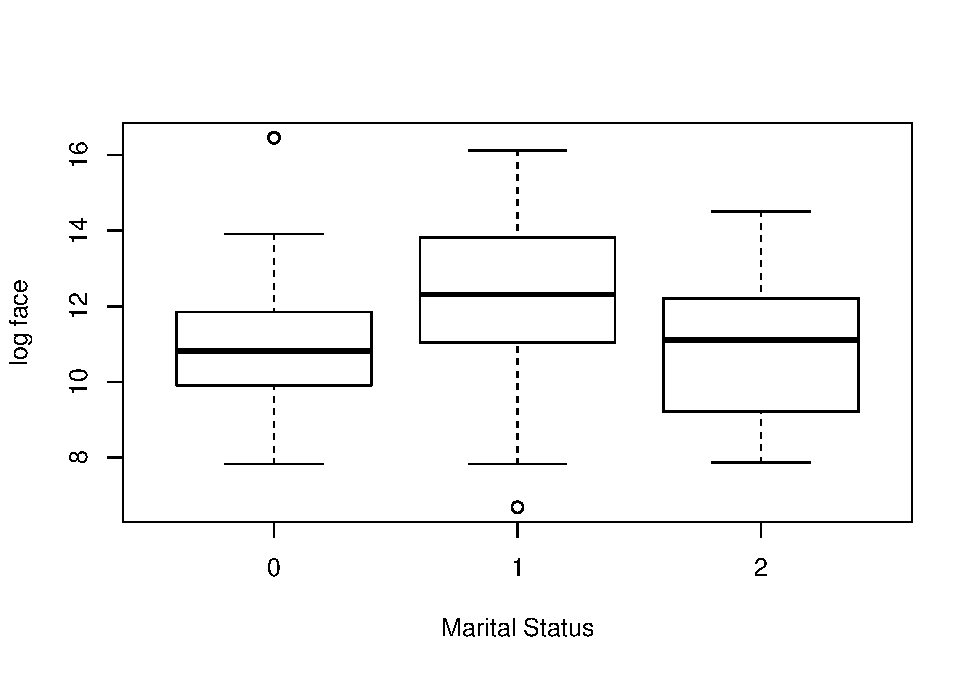
\includegraphics{RegressModelDataCamp_files/figure-latex/unnamed-chunk-121-1.pdf}

\begin{Shaded}
\begin{Highlighting}[]
\KeywordTok{table}\NormalTok{(Term4}\OperatorTok{$}\NormalTok{marstat)}
\CommentTok{#  SUMMARY BY LEVEL OF MARSTAT}
\CommentTok{#library(Rcmdr)}
\CommentTok{#numSummary(Term4[, "logface"], groups = Term4$marstat, statistics = c("mean", "sd"))}
\CommentTok{#numSummary(Term4[, "logface"], statistics = c("mean", "sd"))}
\end{Highlighting}
\end{Shaded}

\begin{verbatim}

  0   1   2 
 57 208  10 
\end{verbatim}

Show Overhead D Details. Regression with a categorical variable

\hypertarget{toggleOver3.4D}{}
\begin{Shaded}
\begin{Highlighting}[]
\NormalTok{Term4}\OperatorTok{$}\NormalTok{marstat <-}\StringTok{ }\KeywordTok{as.factor}\NormalTok{(Term4}\OperatorTok{$}\NormalTok{marstat)}
\NormalTok{Term4}\OperatorTok{$}\NormalTok{marstat <-}\StringTok{ }\KeywordTok{relevel}\NormalTok{(Term4}\OperatorTok{$}\NormalTok{marstat, }\DataTypeTok{ref =} \StringTok{"2"}\NormalTok{)}
\KeywordTok{summary}\NormalTok{(}\KeywordTok{lm}\NormalTok{(logface }\OperatorTok{~}\StringTok{ }\NormalTok{logincome}\OperatorTok{+}\NormalTok{education}\OperatorTok{+}\NormalTok{numhh}\OperatorTok{+}\NormalTok{marstat, }\DataTypeTok{data =}\NormalTok{ Term4))}
\end{Highlighting}
\end{Shaded}

\begin{verbatim}

Call:
lm(formula = logface ~ logincome + education + numhh + marstat, 
    data = Term4)

Residuals:
    Min      1Q  Median      3Q     Max 
-5.8875 -0.8505  0.1124  0.8468  4.5173 

Coefficients:
            Estimate Std. Error t value Pr(>|t|)    
(Intercept)  2.60536    0.95218   2.736 0.006629 ** 
logincome    0.45151    0.07872   5.736 2.61e-08 ***
education    0.20467    0.03862   5.299 2.42e-07 ***
numhh        0.24770    0.06940   3.569 0.000424 ***
marstat0     0.23234    0.53283   0.436 0.663155    
marstat1     0.78941    0.49532   1.594 0.112169    
---
Signif. codes:  0 '***' 0.001 '**' 0.01 '*' 0.05 '.' 0.1 ' ' 1

Residual standard error: 1.513 on 269 degrees of freedom
Multiple R-squared:  0.358, Adjusted R-squared:  0.3461 
F-statistic:    30 on 5 and 269 DF,  p-value: < 2.2e-16
\end{verbatim}

Show Overhead E Details. t-ratios depend on the reference level

\hypertarget{toggleOver3.4E}{}
\[
\begin{array}{l|rr|rr|rr}
 \hline
 & \text{Model 1}&& \text{Model 2}&& \text{Model 3}&\\
 \hline
 \text{Var}& \text{Coef} & \text{t-stat} & \text{Coef} & \text{t-stat} &\text{Coef} & \text{t-stat} \\\hline
logincome & 0.452 & 5.74 & 0.452 & 5.74 & 0.452 & 5.74 \\
education &0.205 & 5.30 &0.205 & 5.30&0.205 & 5.30 \\
numhh     & 0.248 & 3.57 & 0.248 & 3.57 & 0.248 & 3.57 \\\hline
\text{Intercept} & 3.395 & 3.77  & 2.605&  2.74 & 2.838 & 3.34\\
\text{mar=0}    & -0.557 & -2.15&  0.232 &  0.44\\
\text{mar=1} & & & 0.789 & 1.59 & 0.557 & 2.15\\
\text{mar=2}& -0.789 & -1.59 & & & -0.232 & -0.44\\
\hline
\end{array}
\]

\subsection{Exercise. Categorical variables and Wisconsin hospital
costs}\label{exercise.-categorical-variables-and-wisconsin-hospital-costs}

\textbf{Assignment Text}

This exercise examines the impact of various predictors on hospital
charges. Identifying predictors of hospital charges can provide
direction for hospitals, government, insurers and consumers in
controlling these variables that in turn leads to better control of
hospital costs. The data, from 1989, are aggregated by:

\begin{itemize}
\tightlist
\item
  \texttt{drg}, diagnostic related groups of costs,
\item
  \texttt{payer}, type of health care provider (Fee for service, HMO,
  and other), and
\item
  \texttt{hsa}, nine major geographic areas in Wisconsin.
\end{itemize}

Some preliminary analysis of the data has already been done. In this
exercise, we will analyze \texttt{logcharge}, the logarithm of total
hospital charges per number of discharges, in terms of
\texttt{log\_numdschg}, the logarithm of the number of discharges. In
the dataframe \texttt{Hcost} which has been loaded in advance, we
restrict consideration to three types of drgs, numbers 209, 391, and
431.

\textbf{Instructions}

\begin{itemize}
\tightlist
\item
  Fit a basic linear regression model using logarithmic number of
  discharges to predict logarithmic hospital costs and superimposed the
  fitted regression line on the scatter plot.
\item
  Produce a scatter plot of logarithmic number of discharges to predict
  logarithmic hospital costs. Allow plotting symbols and colors to vary
  by diagnostic related group.
\item
  Fit a MLR model using logarithmic number of discharges to predict
  logarithmic hospital costs, allowing intercepts and slopes to vary by
  diagnostic related groups.
\item
  Superimpose the fits from the MLR model on the scatter plot of
  logarithmic number of discharges to predict logarithmic hospital
  costs.
\end{itemize}

eyJsYW5ndWFnZSI6InIiLCJwcmVfZXhlcmNpc2VfY29kZSI6IiNIY29zdCA8LSByZWFkLmNzdihcIkNTVkRhdGFcXFxcV2lzY0hjb3N0cy5jc3ZcIiwgaGVhZGVyID0gVFJVRSlcbkhjb3N0IDwtIHJlYWQuY3N2KFwiaHR0cHM6Ly9hc3NldHMuZGF0YWNhbXAuY29tL3Byb2R1Y3Rpb24vcmVwb3NpdG9yaWVzLzI2MTAvZGF0YXNldHMvMmNjMWUyNzM5YmY4MjcwOTNkYjMxZDdjNGU2ZGNkYzM0OGFjOTg0ZS9XaXNjSGNvc3RzLmNzdlwiLCBoZWFkZXIgPSBUUlVFKVxuSGNvc3QxIDwtIHN1YnNldChIY29zdCwgZHJnID09IDIwOXxkcmcgPT0gMzkxfGRyZyA9PSA0MzApIiwic2FtcGxlIjoiIyBGaXQgYSBiYXNpYyBsaW5lYXIgcmVncmVzc2lvbiBtb2RlbCB1c2luZyBsb2dhcml0aG1pYyBudW1iZXIgb2YgZGlzY2hhcmdlcyB0byBwcmVkaWN0IGxvZ2FyaXRobWljIGhvc3BpdGFsIGNvc3RzIGFuZCBzdXBlcmltcG9zZWQgdGhlIGZpdHRlZCByZWdyZXNzaW9uIGxpbmUgb24gdGhlIHNjYXR0ZXIgcGxvdC5cbmhvc3BfYmxyIDwtIGxtKGxvZ2NoYXJnZX5sb2dfbnVtZHNjaGcsIGRhdGE9SGNvc3QxKVxucGxvdChsb2djaGFyZ2V+bG9nX251bWRzY2hnLCBkYXRhPUhjb3N0MSwgeGxhYiA9IFwibG9nIG51bWJlciBkaXNjaGFyZ2VzXCIsIHlsYWIgPSBcImxvZyBjaGFyZ2VcIilcbmFibGluZShob3NwX2JsciwgY29sPVwicmVkXCIpXG5cbiMgUHJvZHVjZSBhIHNjYXR0ZXIgcGxvdCBvZiBsb2dhcml0aG1pYyBudW1iZXIgb2YgZGlzY2hhcmdlcyB0byBwcmVkaWN0IGxvZ2FyaXRobWljIGhvc3BpdGFsIGNvc3RzLiBBbGxvdyBwbG90dGluZyBzeW1ib2xzIGFuZCBjb2xvcnMgdG8gdmFyeSBieSBkaWFnbm9zdGljIHJlbGF0ZWQgZ3JvdXAuXG5wbG90KGxvZ2NoYXJnZX5sb2dfbnVtZHNjaGcsIGRhdGE9SGNvc3QxLCB4bGFiID0gXCJsb2cgbnVtYmVyIGRpc2NoYXJnZXNcIiwgeWxhYiA9IFwibG9nIGNoYXJnZVwiLFxuICAgIHBjaD0gYXMubnVtZXJpYyhhcy5mYWN0b3IoSGNvc3QxJGRyZykpLCBcbiAgICBjb2wgPSBjKFwicmVkXCIsIFwiYmxhY2tcIiwgXCJibHVlXCIpW2FzLmZhY3RvcihIY29zdDEkZHJnKV0pXG5sZWdlbmQoXCJsZWZ0XCIsIGxlZ2VuZD1jKFwiZHJnIDIwOVwiLFwiZHJnIDM5MVwiLCBcImRyZyA0MzBcIiksIGNvbD1jKFwicmVkXCIsIFwiYmxhY2tcIiwgXCJibHVlXCIpLCBwY2ggPSBjKDEsMiwzKSlcblxuIyBGaXQgYSBNTFIgbW9kZWwgYWxsb3dpbmcgaW50ZXJjZXB0cyBhbmQgc2xvcGVzIHRvIHZhcnkgYnkgZHJnLlxuaG9zcF9tbHIgPC0gbG0obG9nY2hhcmdlfmxvZ19udW1kc2NoZyArIGFzLmZhY3RvcihkcmcpKmxvZ19udW1kc2NoZywgZGF0YT1IY29zdDEpXG5cbiMgU3VwZXJpbXBvc2UgdGhlIGZpdHMgZnJvbSB0aGUgTUxSIG1vZGVsIG9uIHRoZSBzY2F0dGVyIHBsb3Qgb2YgbG9nYXJpdGhtaWMgbnVtYmVyIG9mIGRpc2NoYXJnZXMgdG8gcHJlZGljdCBsb2dhcml0aG1pYyBob3NwaXRhbCBjb3N0cy5cbnBsb3QobG9nY2hhcmdlfmxvZ19udW1kc2NoZywgZGF0YT1IY29zdDEsIHhsYWIgPSBcImxvZyBudW1iZXIgZGlzY2hhcmdlc1wiLCB5bGFiID0gXCJsb2cgY2hhcmdlXCIsXG4gICAgICAgICBwY2g9IGFzLm51bWVyaWMoYXMuZmFjdG9yKEhjb3N0MSRkcmcpKSwgXG4gICAgY29sID0gYyhcInJlZFwiLCBcImJsYWNrXCIsIFwiYmx1ZVwiKVthcy5mYWN0b3IoSGNvc3QxJGRyZyldKVxueHNlcSA8LSBzZXEoMCwxMCxsZW5ndGgub3V0PTEwMClcbmNvZWYgPC0gc3VtbWFyeShob3NwX21scikkY29lZmZpY2llbnRzWywxXVxuZml0MjA5IDwtIGNvZWZbMV0gKyBjb2VmWzJdKnhzZXFcbmxpbmVzKHhzZXEsZml0MjA5LCBjb2w9XCJyZWRcIilcbmZpdDM5MSA8LSBjb2VmWzFdICsgY29lZlszXSArIChjb2VmWzJdICsgY29lZls1XSkqeHNlcVxubGluZXMoeHNlcSxmaXQzOTEsIGNvbD1cImJsYWNrXCIpXG5maXQ0MzAgPC0gY29lZlsxXSArIGNvZWZbNF0gKyAoY29lZlsyXSArIGNvZWZbNl0pKnhzZXFcbmxpbmVzKHhzZXEsZml0NDMwLCBjb2w9XCJibHVlXCIpIiwic29sdXRpb24iOiIjcGFyKG1mcm93ID0gYygyLCAxKSlcbmhvc3BfYmxyIDwtIGxtKGxvZ2NoYXJnZX5sb2dfbnVtZHNjaGcsIGRhdGE9SGNvc3QxKVxucGxvdChsb2djaGFyZ2V+bG9nX251bWRzY2hnLCBkYXRhPUhjb3N0MSwgeGxhYiA9IFwibG9nIG51bWJlciBkaXNjaGFyZ2VzXCIsIHlsYWIgPSBcImxvZyBjaGFyZ2VcIilcbmFibGluZShob3NwX2JsciwgY29sPVwicmVkXCIpXG5cbnBsb3QobG9nY2hhcmdlfmxvZ19udW1kc2NoZywgZGF0YT1IY29zdDEsIHhsYWIgPSBcImxvZyBudW1iZXIgZGlzY2hhcmdlc1wiLCB5bGFiID0gXCJsb2cgY2hhcmdlXCIsXG4gICAgcGNoPSBhcy5udW1lcmljKGFzLmZhY3RvcihIY29zdDEkZHJnKSksIFxuICAgIGNvbCA9IGMoXCJyZWRcIiwgXCJibGFja1wiLCBcImJsdWVcIilbYXMuZmFjdG9yKEhjb3N0MSRkcmcpXSlcbmxlZ2VuZChcImxlZnRcIiwgbGVnZW5kPWMoXCJkcmcgMjA5XCIsXCJkcmcgMzkxXCIsIFwiZHJnIDQzMFwiKSwgY29sPWMoXCJyZWRcIiwgXCJibGFja1wiLCBcImJsdWVcIiksIHBjaCA9IGMoMSwyLDMpKVxuXG5ob3NwX21sciA8LSBsbShsb2djaGFyZ2V+bG9nX251bWRzY2hnICsgYXMuZmFjdG9yKGRyZykqbG9nX251bWRzY2hnLCBkYXRhPUhjb3N0MSlcbiNzdW1tYXJ5KGhvc3BfbWxyKSRjb2VmZmljaWVudHNbLDFdXG5wbG90KGxvZ2NoYXJnZX5sb2dfbnVtZHNjaGcsIGRhdGE9SGNvc3QxLCB4bGFiID0gXCJsb2cgbnVtYmVyIGRpc2NoYXJnZXNcIiwgeWxhYiA9IFwibG9nIGNoYXJnZVwiLFxuICAgICAgICAgcGNoPSBhcy5udW1lcmljKGFzLmZhY3RvcihIY29zdDEkZHJnKSksIFxuICAgIGNvbCA9IGMoXCJyZWRcIiwgXCJibGFja1wiLCBcImJsdWVcIilbYXMuZmFjdG9yKEhjb3N0MSRkcmcpXSlcbnhzZXEgPC0gc2VxKDAsMTAsbGVuZ3RoLm91dD0xMDApXG5jb2VmIDwtIHN1bW1hcnkoaG9zcF9tbHIpJGNvZWZmaWNpZW50c1ssMV1cbmZpdDIwOSA8LSBjb2VmWzFdICsgY29lZlsyXSp4c2VxXG5saW5lcyh4c2VxLGZpdDIwOSwgY29sPVwicmVkXCIpXG5maXQzOTEgPC0gY29lZlsxXSArIGNvZWZbM10gKyAoY29lZlsyXSArIGNvZWZbNV0pKnhzZXFcbmxpbmVzKHhzZXEsZml0MzkxLCBjb2w9XCJibGFja1wiKVxuZml0NDMwIDwtIGNvZWZbMV0gKyBjb2VmWzRdICsgKGNvZWZbMl0gKyBjb2VmWzZdKSp4c2VxXG5saW5lcyh4c2VxLGZpdDQzMCwgY29sPVwiYmx1ZVwiKSIsInNjdCI6InN1Y2Nlc3NfbXNnKFwiQ29uZ3JhdHVsYXRpb25zISBXaGVuIHlvdSBzdXBlcmltcG9zZWQgdGhlIGZpdHMgZnJvbSB0aGUgTUxSIG1vZGVsIG9uIHRoZSBzY2F0dGVyIHBsb3Qgb2YgbG9nYXJpdGhtaWMgbnVtYmVyIG9mIGRpc2NoYXJnZXMgdG8gcHJlZGljdCBsb2dhcml0aG1pYyBob3NwaXRhbCBjb3N0cywgbm90ZSBob3cgc2xvcGVzIGRpZmZlciBkcmFtYXRpY2FsbHkgZnJvbSB0aGUgc2xvcGUgZnJvbSB0aGUgYmFzaWMgbGluZWFyIHJlZ3Jlc3Npb24gbW9kZWwuXCIpIn0=

\section{General linear hypothesis}\label{general-linear-hypothesis}

\begin{center}\rule{0.5\linewidth}{\linethickness}\end{center}

In this section, you learn how to:

\begin{itemize}
\tightlist
\item
  Jointly test the significance of a set of regression coefficients
  using the general linear hypothesis
\item
  Conduct a test of a regression coefficient versus one- or two-side
  alternatives
\end{itemize}

\begin{center}\rule{0.5\linewidth}{\linethickness}\end{center}

\subsection{Video}\label{video-13}

\subsubsection*{Video Overhead Details}\label{video-overhead-details-13}
\addcontentsline{toc}{subsubsection}{Video Overhead Details}

Show Overhead A Details. Testing the significance of a categorical
variable

\hypertarget{toggleOver3.5A}{}
\begin{Shaded}
\begin{Highlighting}[]
\CommentTok{#Term <- read.csv("CSVData\textbackslash{}\textbackslash{}term_life.csv", header = TRUE)}
\NormalTok{Term <-}\StringTok{ }\KeywordTok{read.csv}\NormalTok{(}\StringTok{"https://assets.datacamp.com/production/repositories/2610/datasets/efc64bc2d78cf6b48ad2c3f5e31800cb773de261/term_life.csv"}\NormalTok{, }\DataTypeTok{header =} \OtherTok{TRUE}\NormalTok{)}
\NormalTok{Term1 <-}\StringTok{ }\KeywordTok{subset}\NormalTok{(Term, }\DataTypeTok{subset =}\NormalTok{ face }\OperatorTok{>}\StringTok{ }\DecValTok{0}\NormalTok{)}
\NormalTok{Term4 <-}\StringTok{ }\NormalTok{Term1[,}\KeywordTok{c}\NormalTok{(}\StringTok{"numhh"}\NormalTok{, }\StringTok{"education"}\NormalTok{, }\StringTok{"logincome"}\NormalTok{, }\StringTok{"marstat"}\NormalTok{, }\StringTok{"logface"}\NormalTok{)]}
\NormalTok{Term_mlr1 <-}\StringTok{ }\KeywordTok{lm}\NormalTok{(logface }\OperatorTok{~}\StringTok{ }\NormalTok{logincome }\OperatorTok{+}\StringTok{ }\NormalTok{education }\OperatorTok{+}\StringTok{ }\NormalTok{numhh }\OperatorTok{+}\StringTok{ }\KeywordTok{as.factor}\NormalTok{(Term4}\OperatorTok{$}\NormalTok{marstat), }\DataTypeTok{data =}\NormalTok{ Term4)}
\KeywordTok{anova}\NormalTok{(Term_mlr1)}
\NormalTok{Term_mlr2 <-}\StringTok{ }\KeywordTok{lm}\NormalTok{(logface }\OperatorTok{~}\StringTok{ }\NormalTok{logincome }\OperatorTok{+}\StringTok{ }\NormalTok{education }\OperatorTok{+}\StringTok{ }\NormalTok{numhh, }\DataTypeTok{data =}\NormalTok{ Term4)}

\NormalTok{Fstat <-}\StringTok{ }\NormalTok{(}\KeywordTok{anova}\NormalTok{(Term_mlr2)}\OperatorTok{$}\StringTok{`}\DataTypeTok{Sum Sq}\StringTok{`}\NormalTok{[}\DecValTok{4}\NormalTok{] }\OperatorTok{-}\StringTok{ }\KeywordTok{anova}\NormalTok{(Term_mlr1)}\OperatorTok{$}\StringTok{`}\DataTypeTok{Sum Sq}\StringTok{`}\NormalTok{[}\DecValTok{5}\NormalTok{])}\OperatorTok{/}\NormalTok{(}\DecValTok{2}\OperatorTok{*}\KeywordTok{anova}\NormalTok{(Term_mlr1)}\OperatorTok{$}\StringTok{`}\DataTypeTok{Mean Sq}\StringTok{`}\NormalTok{[}\DecValTok{5}\NormalTok{])}
\NormalTok{Fstat}
\KeywordTok{cat}\NormalTok{(}\StringTok{"p-value is"}\NormalTok{, }\DecValTok{1} \OperatorTok{-}\StringTok{ }\KeywordTok{pf}\NormalTok{(Fstat, }\DataTypeTok{df1 =} \DecValTok{2}\NormalTok{ , }\DataTypeTok{df2 =} \KeywordTok{anova}\NormalTok{(Term_mlr1)}\OperatorTok{$}\NormalTok{Df[}\DecValTok{5}\NormalTok{]))}
\end{Highlighting}
\end{Shaded}

\begin{verbatim}
Analysis of Variance Table

Response: logface
                          Df Sum Sq Mean Sq F value    Pr(>F)    
logincome                  1 222.63 222.629  97.280 < 2.2e-16 ***
education                  1  51.50  51.502  22.504 3.407e-06 ***
numhh                      1  54.34  54.336  23.743 1.883e-06 ***
as.factor(Term4$marstat)   2  14.81   7.406   3.236   0.04085 *  
Residuals                269 615.62   2.289                      
---
Signif. codes:  0 '***' 0.001 '**' 0.01 '*' 0.05 '.' 0.1 ' ' 1
[1] 3.236048
p-value is 0.04085475
\end{verbatim}

Show Overhead B Details. Overview of the general linear hypothesis

\hypertarget{toggleOver3.5B}{}
\begin{itemize}
\tightlist
\item
  The likelihood ratio is a general statistical test procedure that
  compares a model to a subset
\item
  The general linear hypothesis test procedure is similar.

  \begin{itemize}
  \tightlist
  \item
    Start with a (large) linear regression model, examine the fit to a
    set of data
  \item
    Compare this to smaller model that is a subset of the large model.
  \item
    ``Subset'' is the sense that regression coefficients from the small
    model are linear combinations of regression coefficients of the
    large model (e.g., set them to zero)
  \end{itemize}
\item
  Although the likelihood ratio test is more generally available, the
  general linear hypothesis test is more accurate for smaller data sets
  (for normally distributed data)
\end{itemize}

Show Overhead C Details. Procedure for conducting the general linear
hypothesis

\hypertarget{toggleOver3.5C}{}
\begin{itemize}
\tightlist
\item
  Run the full regression and get the error sum of squares and mean
  square error, which we label as \((Error SS)_{full}\) and
  \(s^2_{full}\), respectively.
\item
  Run a reduced regression and get the error sum of squares, labelled
  \((Error SS)_{reduced}\).
\item
  Using \(p\) for the number of linear restrictions, calculate \[
  F-ratio = \frac{(Error SS)_{reduced}-(Error SS)_{full}}{p s^2_{full}} .
  \]
\item
  The probability value is \(p-value = \Pr(F_{p,df} > F-ratio)\) where
  \(F_{p,df}\) has an \emph{F} distribution with degrees of freedom
  \emph{p} and \emph{df}, respectively. (Here, \emph{df} is the degrees
  of freedom for the full model.)
\end{itemize}

Show Overhead D Details. The general linear hypothesis for a single
variable

\hypertarget{toggleOver3.5D}{}
\begin{itemize}
\tightlist
\item
  Suppose that you wish to test the hypothesisthat a regression
  coefficient equals 0.

  \begin{itemize}
  \tightlist
  \item
    One could use the general linear hypothsis procedure with \(p=1\).
  \item
    One could also examine the corresponding \(t-ratio\).
  \item
    Which is correct?
  \end{itemize}
\item
  Both. One can show that \((t-ratio)^2 = F-ratio\), so they are
  equivalent statistics.

  \begin{itemize}
  \tightlist
  \item
    The general linear hypothesis is useful because it can be extended
    to multiple coefficients.
  \item
    The \emph{t-ratio} is useful because it can be used to examine
    one-sided alternative hypotheses.
  \end{itemize}
\end{itemize}

\subsection{Exercise. Hypothesis testing and term
life}\label{exercise.-hypothesis-testing-and-term-life}

\textbf{Assignment Text}

With our \texttt{Term\ life} data, let us compare a model based on the
binary variable that indicates whether a survey respondent is single
versus the more complex marital status, \texttt{marstat}. In principle,
more detailed information is better. But, it may be that the additional
information in \texttt{marstat}, compared to \texttt{single}, does not
help fit the data in a significantly better way.

As part of the preparatory work, the dataframe \texttt{Term4} is
available that includes the binary variable \texttt{single} and the
factor \texttt{marstat}. Moreover, the regression object
\texttt{Term\_mlr} contains information in a multiple linear regression
fit of \texttt{logface} on the base explanatory variables
'logincome\texttt{,}education\texttt{,\ and}numhh`.

\textbf{Instructions}

\begin{itemize}
\tightlist
\item
  Fit a MLR model using the base explanatory variables plus
  \texttt{single} and another model using the base variables plus
  \texttt{marstat}.
\item
  Use the F test to decide whether the additional complexity
  \texttt{marstat} is warranted by calculating the p-value associated
  with this test.
\item
  Fit a MLR model using the base explanatory variables plus
  \texttt{single} interacted with \texttt{logincome} and another model
  using the base variables plus \texttt{marstat} interacted with
  \texttt{logincome}.
\item
  Use the F test to decide whether the additional complexity
  \texttt{marstat} is warranted by calculating the p-value associated
  with this test.
\end{itemize}

\textbf{Hint}

\begin{verbatim}
Here is the code to calculate it by hand
Fstat12 <- (anova(Term_mlr1)$`Sum Sq`[5] - 
              anova(Term_mlr2)$`Sum Sq`[5])/(1*anova(Term_mlr2)$`Mean Sq`[5])
Fstat12
cat("p-value is", 1 - pf(Fstat12, df1 = 1 , df2 = anova(Term_mlr2)$Df[5]))
\end{verbatim}

eyJsYW5ndWFnZSI6InIiLCJwcmVfZXhlcmNpc2VfY29kZSI6IiNUZXJtIDwtIHJlYWQuY3N2KFwiQ1NWRGF0YVxcXFx0ZXJtX2xpZmUuY3N2XCIsIGhlYWRlciA9IFRSVUUpXG5UZXJtIDwtIHJlYWQuY3N2KFwiaHR0cHM6Ly9hc3NldHMuZGF0YWNhbXAuY29tL3Byb2R1Y3Rpb24vcmVwb3NpdG9yaWVzLzI2MTAvZGF0YXNldHMvZWZjNjRiYzJkNzhjZjZiNDhhZDJjM2Y1ZTMxODAwY2I3NzNkZTI2MS90ZXJtX2xpZmUuY3N2XCIsIGhlYWRlciA9IFRSVUUpXG5UZXJtMSA8LSBzdWJzZXQoVGVybSwgc3Vic2V0ID0gZmFjZSA+IDApXG5UZXJtNCA8LSBUZXJtMVssYyhcIm51bWhoXCIsIFwiZWR1Y2F0aW9uXCIsIFwibG9naW5jb21lXCIsIFwibWFyc3RhdFwiLCBcImxvZ2ZhY2VcIildXG5UZXJtNCRzaW5nbGUgPC0gMSooVGVybTQkbWFyc3RhdCA9PSAwKVxuVGVybTQkbWFyc3RhdCA8LSBhcy5mYWN0b3IoVGVybTQkbWFyc3RhdClcblRlcm1fbWxyIDwtIGxtKGxvZ2ZhY2UgfiBsb2dpbmNvbWUgKyBlZHVjYXRpb24gKyBudW1oaCAsIGRhdGEgPSBUZXJtNClcbmFub3ZhKFRlcm1fbWxyKSIsInNhbXBsZSI6IiMgRml0IGEgTUxSIG1vZGVsIHVzaW5nIHRoZSBiYXNlIGV4cGxhbmF0b3J5IHZhcmlhYmxlcyBwbHVzIGBzaW5nbGVgIGFuZCBhbm90aGVyIG1vZGVsIHVzaW5nIHRoZSBiYXNlIHZhcmlhYmxlcyBwbHVzIGBtYXJzdGF0YC5cblRlcm1fbWxyMSA8LSBsbShsb2dmYWNlIH4gbG9naW5jb21lICsgZWR1Y2F0aW9uICsgbnVtaGggK3NpbmdsZSwgZGF0YSA9IFRlcm00KVxuVGVybV9tbHIyIDwtIGxtKGxvZ2ZhY2UgfiBsb2dpbmNvbWUgKyBlZHVjYXRpb24gKyBudW1oaCArbWFyc3RhdCwgZGF0YSA9IFRlcm00KVxuXG4jIFVzZSB0aGUgRiB0ZXN0IHRvIGRlY2lkZSB3aGV0aGVyIHRoZSBhZGRpdGlvbmFsIGNvbXBsZXhpdHkgYG1hcnN0YXRgIGlzIHdhcnJhbnRlZCBieSBjYWxjdWxhdGluZyB0aGUgcC12YWx1ZSBhc3NvY2lhdGVkIHdpdGggdGhpcyB0ZXN0LlxuYW5vdmEoVGVybV9tbHIxLFRlcm1fbWxyMilcblxuIyBGaXQgYSBNTFIgbW9kZWwgdXNpbmcgdGhlIGJhc2UgZXhwbGFuYXRvcnkgdmFyaWFibGVzIHBsdXMgYHNpbmdsZWAgaW50ZXJhY3RlZCB3aXRoIGBsb2dpbmNvbWVgIGFuZCBhbm90aGVyIG1vZGVsIHVzaW5nIHRoZSBiYXNlIHZhcmlhYmxlcyBwbHVzIGBtYXJzdGF0YCBpbnRlcmFjdGVkIHdpdGggYGxvZ2luY29tZWAuXG5UZXJtX21scjMgPC0gbG0obG9nZmFjZSB+IGxvZ2luY29tZSArIGVkdWNhdGlvbiArIG51bWhoICsgc2luZ2xlKmxvZ2luY29tZSwgZGF0YSA9IFRlcm00KVxuVGVybV9tbHI0IDwtIGxtKGxvZ2ZhY2UgfiBsb2dpbmNvbWUgKyBlZHVjYXRpb24gKyBudW1oaCArbWFyc3RhdCpsb2dpbmNvbWUsIGRhdGEgPSBUZXJtNClcblxuIyBVc2UgdGhlIEYgdGVzdCB0byBkZWNpZGUgd2hldGhlciB0aGUgYWRkaXRpb25hbCBjb21wbGV4aXR5IGBtYXJzdGF0YCBpcyB3YXJyYW50ZWQgYnkgY2FsY3VsYXRpbmcgdGhlIHAtdmFsdWUgYXNzb2NpYXRlZCB3aXRoIHRoaXMgdGVzdC5cbmFub3ZhKFRlcm1fbWxyMyxUZXJtX21scjQpIiwic29sdXRpb24iOiJUZXJtX21scjEgPC0gbG0obG9nZmFjZSB+IGxvZ2luY29tZSArIGVkdWNhdGlvbiArIG51bWhoICtzaW5nbGUsIGRhdGEgPSBUZXJtNClcblRlcm1fbWxyMiA8LSBsbShsb2dmYWNlIH4gbG9naW5jb21lICsgZWR1Y2F0aW9uICsgbnVtaGggK21hcnN0YXQsIGRhdGEgPSBUZXJtNClcbmFub3ZhKFRlcm1fbWxyMSxUZXJtX21scjIpXG4jRnN0YXQxMiA8LSAoYW5vdmEoVGVybV9tbHIxKSRgU3VtIFNxYFs1XSAtIFxuIyAgICAgICAgICAgICAgYW5vdmEoVGVybV9tbHIyKSRgU3VtIFNxYFs1XSkvKDEqYW5vdmEoVGVybV9tbHIyKSRgTWVhbiBTcWBbNV0pXG4jRnN0YXQxMlxuI2NhdChcInAtdmFsdWUgaXNcIiwgMSAtIHBmKEZzdGF0MTIsIGRmMSA9IDEgLCBkZjIgPSBhbm92YShUZXJtX21scjIpJERmWzVdKSlcblRlcm1fbWxyMyA8LSBsbShsb2dmYWNlIH4gbG9naW5jb21lICsgZWR1Y2F0aW9uICsgbnVtaGggKyBzaW5nbGUqbG9naW5jb21lLCBkYXRhID0gVGVybTQpXG5UZXJtX21scjQgPC0gbG0obG9nZmFjZSB+IGxvZ2luY29tZSArIGVkdWNhdGlvbiArIG51bWhoICttYXJzdGF0KmxvZ2luY29tZSwgZGF0YSA9IFRlcm00KVxuYW5vdmEoVGVybV9tbHIzLFRlcm1fbWxyNCkiLCJzY3QiOiJleCgpICU+JSBjaGVja19vYmplY3QoXCJUZXJtX21scjFcIikgJT4lIGNoZWNrX2VxdWFsKClcbmV4KCkgJT4lIGNoZWNrX29iamVjdChcIlRlcm1fbWxyMlwiKSAlPiUgY2hlY2tfZXF1YWwoKVxuZXgoKSAlPiUgY2hlY2tfZnVuY3Rpb24oXCJhbm92YVwiLGluZGV4PTEpICU+JSBjaGVja19yZXN1bHQoKSAlPiUgY2hlY2tfZXF1YWwoKVxuZXgoKSAlPiUgY2hlY2tfb2JqZWN0KFwiVGVybV9tbHIzXCIpICU+JSBjaGVja19lcXVhbCgpXG5leCgpICU+JSBjaGVja19vYmplY3QoXCJUZXJtX21scjRcIikgJT4lIGNoZWNrX2VxdWFsKClcbmV4KCkgJT4lIGNoZWNrX2Z1bmN0aW9uKFwiYW5vdmFcIixpbmRleD0yKSAlPiUgY2hlY2tfcmVzdWx0KCkgJT4lIGNoZWNrX2VxdWFsKClcbnN1Y2Nlc3NfbXNnKFwiQ29uZ3JhdHVsYXRpb25zISBIeXBvdGhlc2lzIHRlc3RpbmcgaXMgYSBwcmltYXJ5IHRvb2wgZm9yICAnaW5mZXJyaW5nJyBhYm91dCB0aGUgcmVhbCB3b3JsZCB7aW4gY29udHJhc3QgdG8gbWF0aGVtYXRpY2FsICdkZWR1Y3Rpb24nLn0gTW9yZW92ZXIsIGFzIHdlIHdpbGwgc2VlIGluIHRoZSBuZXh0IGNoYXB0ZXIsIGl0IGNhbiBhbHNvIGJlIHVzZWQgdG8gZGV2ZWxvcCBhIG1vZGVsLlwiKSJ9

\subsection{Exercise. Hypothesis testing and Wisconsin hospital
costs}\label{exercise.-hypothesis-testing-and-wisconsin-hospital-costs}

\textbf{Assignment Text}

In a previous exercise, you were introduced to a dataset with hospital
charges aggregated by:

\begin{itemize}
\tightlist
\item
  \texttt{drg}, diagnostic related groups of costs,
\item
  \texttt{payer}, type of health care provider (Fee for service, HMO,
  and other), and
\item
  \texttt{hsa}, nine major geographic areas.
\end{itemize}

We continue our analysis of the outcome variable \texttt{logcharge}, the
logarithm of total hospital charges per number of discharges, in terms
of \texttt{log\_numdschg}, the logarithm of the number of discharges, as
well as the three categorical variables used in the aggregation. As
before, we restrict consideration to three types of drgs, numbers 209,
391, and 431 that has been preloaded in the dataframe \texttt{Hcost1}.

\textbf{Instructions}

\begin{itemize}
\tightlist
\item
  Fit a basic linear regression model using logarithmic hospital costs
  as the outcome variable and explanatory variable logarithmic number of
  discharges.
\item
  Fit a MLR model using logarithmic hospital costs as the outcome
  variable and explanatory variables logarithmic number of discharges
  and the categorical variable diagnostic related group. Identify the
  \emph{F} statistic and \emph{p} value that test the importance of
  diagnostic related group.
\item
  Fit a MLR model using logarithmic hospital costs as the outcome
  variable and explanatory variable logarithmic number of discharges
  interacted with diagnostic related group. Identify the \emph{F}
  statistic and \emph{p} value that test the importance of diagnostic
  related group interaction with logarithmic number of discharges.
\item
  Calculate a coefficient of determination, \(R^2\), for each of these
  models as well as for a model using logarithmic number of discharges
  and categorical variable \texttt{hsa} as predictors.
\end{itemize}

eyJsYW5ndWFnZSI6InIiLCJwcmVfZXhlcmNpc2VfY29kZSI6IiNIY29zdCA8LSByZWFkLmNzdihcIkNTVkRhdGFcXFxcV2lzY0hjb3N0cy5jc3ZcIiwgaGVhZGVyID0gVFJVRSlcbkhjb3N0IDwtIHJlYWQuY3N2KFwiaHR0cHM6Ly9hc3NldHMuZGF0YWNhbXAuY29tL3Byb2R1Y3Rpb24vcmVwb3NpdG9yaWVzLzI2MTAvZGF0YXNldHMvMmNjMWUyNzM5YmY4MjcwOTNkYjMxZDdjNGU2ZGNkYzM0OGFjOTg0ZS9XaXNjSGNvc3RzLmNzdlwiLCBoZWFkZXIgPSBUUlVFKVxuSGNvc3QxIDwtIHN1YnNldChIY29zdCwgZHJnID09IDIwOXxkcmcgPT0gMzkxfGRyZyA9PSA0MzApIiwic2FtcGxlIjoiIyBSZWdyZXNzIGxvZyBjaGFyZ2VzIG9uIGxvZyBudW1iZXIgb2YgZGlzY2hhcmdlc1xuaG9zcF9ibHIgPC0gbG0obG9nY2hhcmdlIH4gbG9nX251bWRzY2hnICwgZGF0YT1IY29zdDEpXG5hbm92YShob3NwX2JscilcblxuIyBSZWdyZXNzIGxvZyBjaGFyZ2VzIG9uIGxvZyBudW1iZXIgb2YgZGlzY2hhcmdlcyBhbmQgZHJnLiBJZGVudGlmeSB0aGUgKkYqIHN0YXRpc3RpYyBhbmQgKnAqIHZhbHVlIHRoYXQgdGVzdCB0aGUgaW1wb3J0YW5jZSBvZiBkaWFnbm9zdGljIHJlbGF0ZWQgZ3JvdXAuXG5ob3NwX21scjEgPC0gbG0obG9nY2hhcmdlIH4gbG9nX251bWRzY2hnICsgYXMuZmFjdG9yKGRyZyksIGRhdGE9SGNvc3QxKVxuYW5vdmEoaG9zcF9tbHIxKVxuXG4jIFJlZ3Jlc3MgbG9nIGNoYXJnZXMgb24gdGhlIGludGVyYWN0aW9uIG9mIGxvZyBudW1iZXIgb2YgZGlzY2hhcmdlcyBhbmQgZHJnLiBcbmhvc3BfbWxyMiA8LSBsbShsb2djaGFyZ2UgfiBsb2dfbnVtZHNjaGcgKyBhcy5mYWN0b3IoZHJnKSpsb2dfbnVtZHNjaGcsIGRhdGE9SGNvc3QxKVxuYW5vdmEoaG9zcF9tbHIyKVxuXG4jIENhbGN1bGF0ZSBhIGNvZWZmaWNpZW50IG9mIGRldGVybWluYXRpb24sICRSXjIkLCBmb3IgZWFjaCBvZiB0aGVzZSBtb2RlbHMgYXMgd2VsbCBhcyBmb3IgYSBtb2RlbCB1c2luZyBsb2dhcml0aG1pYyBudW1iZXIgb2YgZGlzY2hhcmdlcyBhbmQgY2F0ZWdvcmljYWwgdmFyaWFibGUgYGhzYWAgYXMgcHJlZGljdG9ycy5cbnN1bW1hcnkoaG9zcF9ibHIpJHIuc3F1YXJlZFxuc3VtbWFyeShob3NwX21scjEpJHIuc3F1YXJlZFxuc3VtbWFyeShob3NwX21scjIpJHIuc3F1YXJlZFxuXG5ob3NwX21scjMgPC0gbG0obG9nY2hhcmdlIH4gbG9nX251bWRzY2hnICsgYXMuZmFjdG9yKGhzYSkqbG9nX251bWRzY2hnLCBkYXRhPUhjb3N0MSlcbnN1bW1hcnkoaG9zcF9tbHIzKSRyLnNxdWFyZWQiLCJzb2x1dGlvbiI6Imhvc3BfYmxyIDwtIGxtKGxvZ2NoYXJnZSB+IGxvZ19udW1kc2NoZyAsIGRhdGE9SGNvc3QxKVxuYW5vdmEoaG9zcF9ibHIpXG5ob3NwX21scjEgPC0gbG0obG9nY2hhcmdlIH4gbG9nX251bWRzY2hnICsgYXMuZmFjdG9yKGRyZyksIGRhdGE9SGNvc3QxKVxuYW5vdmEoaG9zcF9tbHIxKVxuaG9zcF9tbHIyIDwtIGxtKGxvZ2NoYXJnZSB+IGxvZ19udW1kc2NoZyArIGFzLmZhY3RvcihkcmcpKmxvZ19udW1kc2NoZywgZGF0YT1IY29zdDEpXG5hbm92YShob3NwX21scjIpXG5zdW1tYXJ5KGhvc3BfYmxyKSRyLnNxdWFyZWRcbnN1bW1hcnkoaG9zcF9tbHIxKSRyLnNxdWFyZWRcbnN1bW1hcnkoaG9zcF9tbHIyKSRyLnNxdWFyZWRcblxuaG9zcF9tbHIzIDwtIGxtKGxvZ2NoYXJnZSB+IGxvZ19udW1kc2NoZyArIGFzLmZhY3Rvcihoc2EpKmxvZ19udW1kc2NoZywgZGF0YT1IY29zdDEpXG5zdW1tYXJ5KGhvc3BfbWxyMykkci5zcXVhcmVkIiwic2N0Ijoic3VjY2Vzc19tc2coXCJDb25ncmF0dWxhdGlvbnMhIEJ5IGV4YW1pbmluZyB0aGUgY29lZmZpY2llbnRzIG9mIGRldGVybWluYXRpb24sICRSXjIkLCBmb3IgZWFjaCBvZiB0aGVzZSBtb2RlbHMsIHlvdSBzZWUgdGhhdCB0aGlzIHByb3ZpZGVzIG9uZSBwaWVjZSBvZiBldmlkZW5jZSB0aGF0IHRoZSBgaHNhYCBpcyBhIGZhciBwb29yZXIgcHJlZGljdG9yIG9mIGNvc3RzIHRoYW4gYGRyZ2AuXCIpIn0=

\subsection{Exercise. Hypothesis testing and auto
claims}\label{exercise.-hypothesis-testing-and-auto-claims}

\textbf{Assignment Text}

As an actuarial analyst, you are working with a large insurance company
to help them understand their claims distribution for their private
passenger automobile policies. You have available claims data for a
recent year, consisting of:

\begin{itemize}
\tightlist
\item
  \texttt{state}: codes 01 through 17 used, with each code randomly
  assigned to an actual individual state
\item
  \texttt{class}: rating class of operator, based on age, gender,
  marital status, and use of vehicle
\item
  \texttt{gender}: operator gender
\item
  \texttt{age}: operator age
\item
  \texttt{paid}: amount paid to settle and close a claim.
\end{itemize}

You are focusing on older drivers, 50 and higher, for which there are
\emph{n} = 6,773 claims available.

\textbf{Instructions}

\begin{enumerate}
\def\labelenumi{\alph{enumi}.}
\item
  Run a regression of \texttt{logpaid} on \texttt{age}. Is \texttt{age}
  a statistically significant variable? To respond to this question, use
  a formal test of hypothesis. State your null and alternative
  hypotheses, decision-making criterion, and your decision-making rule.
  Also comment on the goodness of fit of this variable.
\item
  Consider using class as a single explanatory variable. Use the one
  factor to estimate the model and respond to the following questions.

  b (i). What is the point estimate of claims in class C7, drivers
  50-69, driving to work or school, less than 30 miles per week with
  annual mileage under 7500, in natural logarithmic units?

  b (ii). Determine the corresponding 95\% confidence interval of
  expected claims, in natural logarithmic units.

  b (iii). Convert the 95\% confidence interval of expected claims that
  you determined in part b(ii) to dollars.
\item
  Run a regression of \texttt{logpaid} on \texttt{age}, \texttt{gender}
  and the categorical variables \texttt{state} and \texttt{class}.

  c (i). Is \texttt{gender} a statistically significant variable? To
  respond to this question, use a formal test of hypothesis. State your
  null and alternative hypotheses, decision-making criterion, and your
  decision-making rule.

  c (ii). Is \texttt{class} a statistically significant variable? To
  respond to this question, use a formal test of hypothesis. State your
  null and alternative hypotheses, decision-making criterion, and your
  decision-making rule.

  c (iii). Use the model to provide a point estimate of claims in
  dollars (not log dollars) for a male age 60 in STATE 2 in
  \texttt{class} C7.

  c (iv). Write down the coefficient associated with \texttt{class} C7
  and interpret this coefficient.
\end{enumerate}

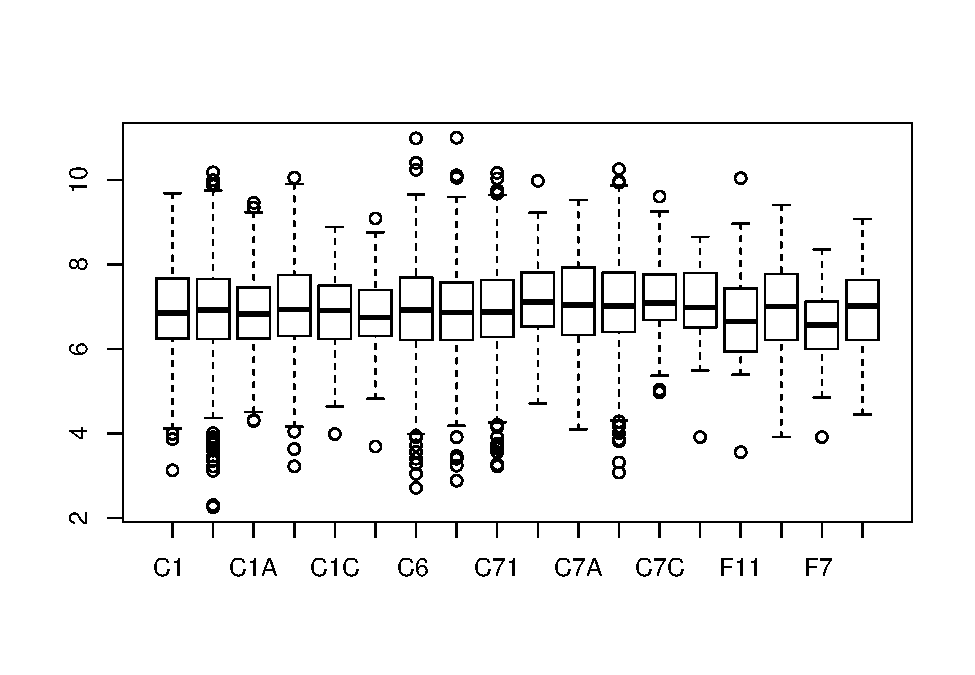
\includegraphics{RegressModelDataCamp_files/figure-latex/unnamed-chunk-136-1.pdf}
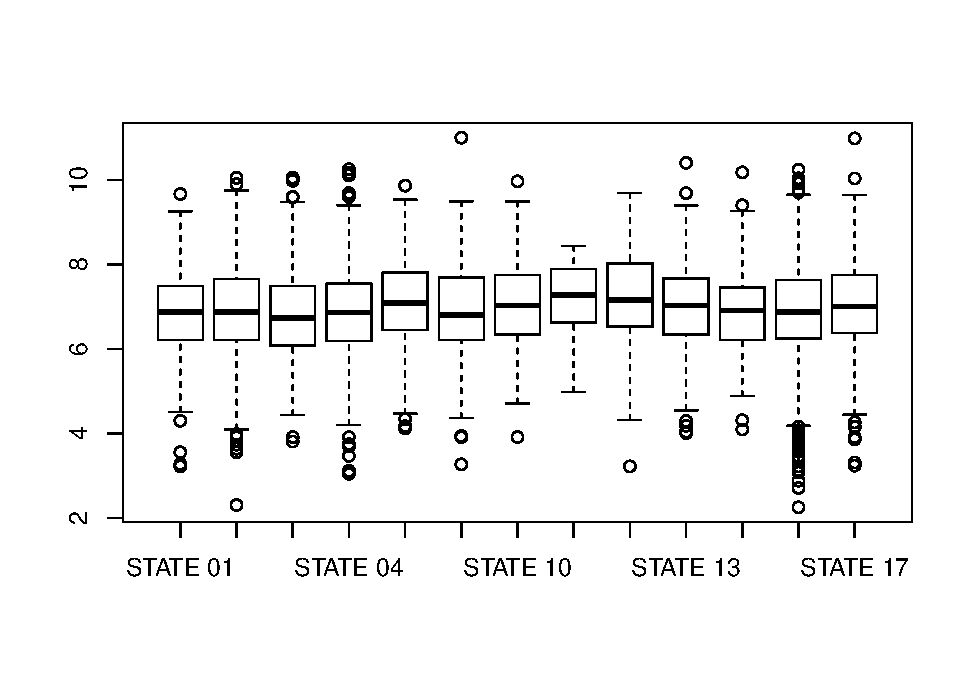
\includegraphics{RegressModelDataCamp_files/figure-latex/unnamed-chunk-136-2.pdf}

\begin{verbatim}

Call:
lm(formula = logpaid ~ class, data = AutoC)

Residuals:
    Min      1Q  Median      3Q     Max 
-4.7002 -0.6912 -0.0437  0.7128  4.1009 

Coefficients:
             Estimate Std. Error t value Pr(>|t|)    
(Intercept)  6.940938   0.039699 174.838   <2e-16 ***
classC11     0.010564   0.050696   0.208   0.8349    
classC1A    -0.075432   0.128202  -0.588   0.5563    
classC1B     0.057420   0.065380   0.878   0.3798    
classC1C    -0.154707   0.178007  -0.869   0.3848    
classC2     -0.139442   0.142595  -0.978   0.3282    
classC6     -0.015057   0.053217  -0.283   0.7772    
classC7     -0.039775   0.053191  -0.748   0.4546    
classC71     0.012730   0.050887   0.250   0.8025    
classC72     0.241716   0.122626   1.971   0.0487 *  
classC7A     0.122755   0.108174   1.135   0.2565    
classC7B     0.131512   0.056956   2.309   0.0210 *  
classC7C     0.302596   0.125307   2.415   0.0158 *  
classF1      0.062962   0.202561   0.311   0.7559    
classF11    -0.136891   0.173726  -0.788   0.4307    
classF6     -0.030546   0.094148  -0.324   0.7456    
classF7     -0.363874   0.144807  -2.513   0.0120 *  
classF71    -0.005476   0.117810  -0.046   0.9629    
---
Signif. codes:  0 '***' 0.001 '**' 0.01 '*' 0.05 '.' 0.1 ' ' 1

Residual standard error: 1.07 on 6755 degrees of freedom
Multiple R-squared:  0.005048,  Adjusted R-squared:  0.002544 
F-statistic: 2.016 on 17 and 6755 DF,  p-value: 0.00786


Call:
lm(formula = logpaid ~ state, data = AutoC)

Residuals:
    Min      1Q  Median      3Q     Max 
-4.6555 -0.6847 -0.0415  0.7005  4.0788 

Coefficients:
              Estimate Std. Error t value Pr(>|t|)    
(Intercept)    6.82202    0.08286  82.328  < 2e-16 ***
stateSTATE 02  0.11739    0.08878   1.322 0.186133    
stateSTATE 03  0.02224    0.10071   0.221 0.825246    
stateSTATE 04  0.05195    0.09262   0.561 0.574893    
stateSTATE 06  0.30735    0.09327   3.295 0.000988 ***
stateSTATE 07  0.10127    0.10537   0.961 0.336562    
stateSTATE 10  0.21247    0.10486   2.026 0.042787 *  
stateSTATE 11  0.17462    0.36540   0.478 0.632751    
stateSTATE 12  0.40876    0.10715   3.815 0.000138 ***
stateSTATE 13  0.21792    0.11111   1.961 0.049890 *  
stateSTATE 14  0.06485    0.11667   0.556 0.578297    
stateSTATE 15  0.08479    0.08596   0.986 0.323956    
stateSTATE 17  0.22406    0.09585   2.338 0.019442 *  
---
Signif. codes:  0 '***' 0.001 '**' 0.01 '*' 0.05 '.' 0.1 ' ' 1

Residual standard error: 1.068 on 6760 degrees of freedom
Multiple R-squared:  0.008109,  Adjusted R-squared:  0.006348 
F-statistic: 4.606 on 12 and 6760 DF,  p-value: 1.749e-07

Analysis of Variance Table

Response: logpaid
            Df Sum Sq Mean Sq F value    Pr(>F)    
state       12   63.0  5.2495  4.6055 1.749e-07 ***
Residuals 6760 7705.2  1.1398                      
---
Signif. codes:  0 '***' 0.001 '**' 0.01 '*' 0.05 '.' 0.1 ' ' 1

Call:
lm(formula = logpaid ~ class + state + age + gender, data = AutoC)

Residuals:
    Min      1Q  Median      3Q     Max 
-4.7266 -0.6802 -0.0433  0.7072  4.1809 

Coefficients:
               Estimate Std. Error t value Pr(>|t|)    
(Intercept)    6.974923   0.140144  49.770  < 2e-16 ***
classC11       0.055573   0.051695   1.075 0.282410    
classC1A      -0.110591   0.128238  -0.862 0.388506    
classC1B       0.022671   0.066388   0.341 0.732740    
classC1C      -0.160355   0.178056  -0.901 0.367842    
classC2       -0.183935   0.142784  -1.288 0.197719    
classC6        0.057560   0.058767   0.979 0.327395    
classC7       -0.021854   0.054531  -0.401 0.688605    
classC71       0.024622   0.053049   0.464 0.642569    
classC72       0.260057   0.123451   2.107 0.035192 *  
classC7A       0.119315   0.108879   1.096 0.273183    
classC7B       0.124196   0.059098   2.102 0.035634 *  
classC7C       0.299023   0.126300   2.368 0.017934 *  
classF1        0.130054   0.202380   0.643 0.520491    
classF11      -0.058684   0.174394  -0.337 0.736503    
classF6        0.068612   0.098270   0.698 0.485079    
classF7       -0.309974   0.145271  -2.134 0.032898 *  
classF71       0.029459   0.118848   0.248 0.804239    
stateSTATE 02  0.098538   0.089280   1.104 0.269765    
stateSTATE 03  0.006302   0.101050   0.062 0.950272    
stateSTATE 04  0.019266   0.093712   0.206 0.837118    
stateSTATE 06  0.283853   0.094105   3.016 0.002568 ** 
stateSTATE 07  0.076593   0.106361   0.720 0.471475    
stateSTATE 10  0.181802   0.105448   1.724 0.084739 .  
stateSTATE 11  0.172272   0.365574   0.471 0.637487    
stateSTATE 12  0.388006   0.108333   3.582 0.000344 ***
stateSTATE 13  0.188491   0.111980   1.683 0.092371 .  
stateSTATE 14  0.068141   0.116720   0.584 0.559373    
stateSTATE 15  0.065570   0.086624   0.757 0.449110    
stateSTATE 17  0.199398   0.096914   2.057 0.039680 *  
age           -0.003021   0.001690  -1.787 0.073914 .  
genderM        0.038953   0.026907   1.448 0.147747    
---
Signif. codes:  0 '***' 0.001 '**' 0.01 '*' 0.05 '.' 0.1 ' ' 1

Residual standard error: 1.066 on 6741 degrees of freedom
Multiple R-squared:  0.01365,   Adjusted R-squared:  0.009113 
F-statistic: 3.009 on 31 and 6741 DF,  p-value: 4.354e-08

Analysis of Variance Table

Response: logpaid
            Df Sum Sq Mean Sq F value    Pr(>F)    
class       17   39.2  2.3066  2.0293  0.007346 ** 
state       12   61.0  5.0841  4.4728 3.354e-07 ***
age          1    3.4  3.4284  3.0162  0.082480 .  
gender       1    2.4  2.3823  2.0958  0.147747    
Residuals 6741 7662.2  1.1367                      
---
Signif. codes:  0 '***' 0.001 '**' 0.01 '*' 0.05 '.' 0.1 ' ' 1
\end{verbatim}

\textbf{Submission Correctness Tests (SCT)}

success\_msg(``Congratulations!'')

\chapter{Variable Selection}\label{variable-selection}

\textbf{Chapter description}

This chapter describes tools and techniques to help you select variables
to enter into a linear regression model, beginning with an iterative
model selection process. In applications with many potential explanatory
variables, automatic variable selection procedures are available that
will help you quickly evaluate many models. Nonetheless, automatic
procedures have serious limitations including the inability to account
properly for nonlinearities such as the impact of unusual points; this
chapter expands upon the Chapter 2 discussion of unusual points. It also
describes collinearity, a common feature of regression data where
explanatory variables are linearly related to one another. Other topics
that impact variable selection, including out-of-sample validation, are
also introduced.

\section{An iterative approach to data analysis and
modeling}\label{an-iterative-approach-to-data-analysis-and-modeling}

\begin{center}\rule{0.5\linewidth}{\linethickness}\end{center}

In this section, you learn how to:

\begin{itemize}
\tightlist
\item
  Describe the iterative approach to data analysis and modeling.
\end{itemize}

\begin{center}\rule{0.5\linewidth}{\linethickness}\end{center}

\subsection{Video}\label{video-14}

\subsubsection*{Video Overhead Details}\label{video-overhead-details-14}
\addcontentsline{toc}{subsubsection}{Video Overhead Details}

Show Overhead A Details. Iterative approach

\hypertarget{toggleOver4.1A}{}
\begin{itemize}
\tightlist
\item
  Model formulation stage
\item
  Fitting
\item
  Diagnostic checking - the data and model must be consistent with one
  another before additional inferences can be made.
\end{itemize}

\begin{Shaded}
\begin{Highlighting}[]
\KeywordTok{plot.new}\NormalTok{()}
\KeywordTok{par}\NormalTok{(}\DataTypeTok{mar=}\KeywordTok{c}\NormalTok{(}\DecValTok{0}\NormalTok{,}\DecValTok{0}\NormalTok{,}\DecValTok{0}\NormalTok{,}\DecValTok{0}\NormalTok{), }\DataTypeTok{cex=}\FloatTok{0.9}\NormalTok{)}
\KeywordTok{plot.window}\NormalTok{(}\DataTypeTok{xlim=}\KeywordTok{c}\NormalTok{(}\DecValTok{0}\NormalTok{,}\DecValTok{18}\NormalTok{),}\DataTypeTok{ylim=}\KeywordTok{c}\NormalTok{(}\OperatorTok{-}\DecValTok{5}\NormalTok{,}\DecValTok{5}\NormalTok{))}

\KeywordTok{text}\NormalTok{(}\DecValTok{1}\NormalTok{,}\DecValTok{3}\NormalTok{,}\DataTypeTok{labels=}\StringTok{"DATA"}\NormalTok{,}\DataTypeTok{adj=}\DecValTok{0}\NormalTok{, }\DataTypeTok{cex=}\FloatTok{0.8}\NormalTok{)}
\KeywordTok{text}\NormalTok{(}\DecValTok{1}\NormalTok{,}\DecValTok{0}\NormalTok{,}\DataTypeTok{labels=}\StringTok{"PLOTS"}\NormalTok{,}\DataTypeTok{adj=}\DecValTok{0}\NormalTok{, }\DataTypeTok{cex=}\FloatTok{0.8}\NormalTok{)}
\KeywordTok{text}\NormalTok{(}\DecValTok{1}\NormalTok{,}\OperatorTok{-}\DecValTok{3}\NormalTok{,}\DataTypeTok{labels=}\StringTok{"THEORY"}\NormalTok{,}\DataTypeTok{adj=}\DecValTok{0}\NormalTok{, }\DataTypeTok{cex=}\FloatTok{0.8}\NormalTok{)}
\KeywordTok{text}\NormalTok{(}\FloatTok{3.9}\NormalTok{,}\DecValTok{0}\NormalTok{,}\DataTypeTok{labels=}\StringTok{"MODEL}\CharTok{\textbackslash{}n}\StringTok{FORMULATION"}\NormalTok{,}\DataTypeTok{adj=}\DecValTok{0}\NormalTok{, }\DataTypeTok{cex=}\FloatTok{0.8}\NormalTok{)}
\KeywordTok{text}\NormalTok{(}\FloatTok{8.1}\NormalTok{,}\DecValTok{0}\NormalTok{,}\DataTypeTok{labels=}\StringTok{"FITTING"}\NormalTok{,}\DataTypeTok{adj=}\DecValTok{0}\NormalTok{, }\DataTypeTok{cex=}\FloatTok{0.8}\NormalTok{)}
\KeywordTok{text}\NormalTok{(}\DecValTok{11}\NormalTok{,}\DecValTok{0}\NormalTok{,}\DataTypeTok{labels=}\StringTok{"DIAGNOSTIC}\CharTok{\textbackslash{}n}\StringTok{CHECKING"}\NormalTok{,}\DataTypeTok{adj=}\DecValTok{0}\NormalTok{, }\DataTypeTok{cex=}\FloatTok{0.8}\NormalTok{)}
\KeywordTok{text}\NormalTok{(}\DecValTok{15}\NormalTok{,}\DecValTok{0}\NormalTok{,}\DataTypeTok{labels=}\StringTok{"INFERENCE"}\NormalTok{,}\DataTypeTok{adj=}\DecValTok{0}\NormalTok{, }\DataTypeTok{cex=}\FloatTok{0.8}\NormalTok{)}
\KeywordTok{text}\NormalTok{(}\FloatTok{14.1}\NormalTok{,}\FloatTok{0.5}\NormalTok{,}\DataTypeTok{labels=}\StringTok{"OK"}\NormalTok{,}\DataTypeTok{adj=}\DecValTok{0}\NormalTok{, }\DataTypeTok{cex=}\FloatTok{0.6}\NormalTok{)}

\KeywordTok{rect}\NormalTok{(}\FloatTok{0.8}\NormalTok{,}\FloatTok{2.0}\NormalTok{,}\FloatTok{2.6}\NormalTok{,}\FloatTok{4.0}\NormalTok{)}
\KeywordTok{arrows}\NormalTok{(}\FloatTok{1.7}\NormalTok{,}\FloatTok{2.0}\NormalTok{,}\FloatTok{1.7}\NormalTok{,}\FloatTok{1.0}\NormalTok{,}\DataTypeTok{code=}\DecValTok{2}\NormalTok{,}\DataTypeTok{lwd=}\DecValTok{2}\NormalTok{,}\DataTypeTok{angle=}\DecValTok{25}\NormalTok{,}\DataTypeTok{length=}\FloatTok{0.10}\NormalTok{)}
\KeywordTok{rect}\NormalTok{(}\FloatTok{0.8}\NormalTok{,}\OperatorTok{-}\FloatTok{1.0}\NormalTok{,}\FloatTok{2.6}\NormalTok{,}\FloatTok{1.0}\NormalTok{)}
\KeywordTok{arrows}\NormalTok{(}\FloatTok{1.7}\NormalTok{,}\OperatorTok{-}\FloatTok{2.0}\NormalTok{,}\FloatTok{1.7}\NormalTok{,}\OperatorTok{-}\FloatTok{1.0}\NormalTok{,}\DataTypeTok{code=}\DecValTok{2}\NormalTok{,}\DataTypeTok{lwd=}\DecValTok{2}\NormalTok{,}\DataTypeTok{angle=}\DecValTok{25}\NormalTok{,}\DataTypeTok{length=}\FloatTok{0.10}\NormalTok{)}
\KeywordTok{rect}\NormalTok{(}\FloatTok{0.8}\NormalTok{,}\OperatorTok{-}\FloatTok{4.0}\NormalTok{,}\FloatTok{2.6}\NormalTok{,}\OperatorTok{-}\FloatTok{2.0}\NormalTok{)}

\KeywordTok{arrows}\NormalTok{(}\FloatTok{2.6}\NormalTok{,}\DecValTok{0}\NormalTok{,}\FloatTok{3.2}\NormalTok{,}\DecValTok{0}\NormalTok{,}\DataTypeTok{code=}\DecValTok{2}\NormalTok{,}\DataTypeTok{lwd=}\DecValTok{2}\NormalTok{,}\DataTypeTok{angle=}\DecValTok{25}\NormalTok{,}\DataTypeTok{length=}\FloatTok{0.10}\NormalTok{)}

\NormalTok{x<-}\KeywordTok{c}\NormalTok{(}\DecValTok{5}\NormalTok{,}\FloatTok{7.0}\NormalTok{,}\DecValTok{5}\NormalTok{,}\FloatTok{3.2}\NormalTok{)}
\NormalTok{y<-}\KeywordTok{c}\NormalTok{(}\DecValTok{2}\NormalTok{,}\DecValTok{0}\NormalTok{,}\OperatorTok{-}\DecValTok{2}\NormalTok{,}\DecValTok{0}\NormalTok{)}
\KeywordTok{polygon}\NormalTok{(x,y)}
\KeywordTok{arrows}\NormalTok{(}\FloatTok{7.0}\NormalTok{,}\DecValTok{0}\NormalTok{,}\FloatTok{8.0}\NormalTok{,}\DecValTok{0}\NormalTok{,}\DataTypeTok{code=}\DecValTok{2}\NormalTok{,}\DataTypeTok{lwd=}\DecValTok{2}\NormalTok{,}\DataTypeTok{angle=}\DecValTok{25}\NormalTok{,}\DataTypeTok{length=}\FloatTok{0.10}\NormalTok{)}

\KeywordTok{rect}\NormalTok{(}\FloatTok{8.0}\NormalTok{,}\OperatorTok{-}\FloatTok{1.0}\NormalTok{,}\FloatTok{9.7}\NormalTok{,}\FloatTok{1.0}\NormalTok{)}
\KeywordTok{arrows}\NormalTok{(}\FloatTok{9.7}\NormalTok{,}\DecValTok{0}\NormalTok{,}\FloatTok{10.2}\NormalTok{,}\DecValTok{0}\NormalTok{,}\DataTypeTok{code=}\DecValTok{2}\NormalTok{,}\DataTypeTok{lwd=}\DecValTok{2}\NormalTok{,}\DataTypeTok{angle=}\DecValTok{25}\NormalTok{,}\DataTypeTok{length=}\FloatTok{0.10}\NormalTok{)}

\NormalTok{x1<-}\KeywordTok{c}\NormalTok{(}\DecValTok{12}\NormalTok{,}\FloatTok{14.0}\NormalTok{,}\DecValTok{12}\NormalTok{,}\FloatTok{10.2}\NormalTok{)}
\NormalTok{y1<-}\KeywordTok{c}\NormalTok{(}\DecValTok{2}\NormalTok{,}\DecValTok{0}\NormalTok{,}\OperatorTok{-}\DecValTok{2}\NormalTok{,}\DecValTok{0}\NormalTok{)}
\KeywordTok{polygon}\NormalTok{(x1,y1)}
\KeywordTok{arrows}\NormalTok{(}\FloatTok{14.0}\NormalTok{,}\DecValTok{0}\NormalTok{,}\FloatTok{14.8}\NormalTok{,}\DecValTok{0}\NormalTok{,}\DataTypeTok{code=}\DecValTok{2}\NormalTok{,}\DataTypeTok{lwd=}\DecValTok{2}\NormalTok{,}\DataTypeTok{angle=}\DecValTok{25}\NormalTok{,}\DataTypeTok{length=}\FloatTok{0.10}\NormalTok{)}

\KeywordTok{rect}\NormalTok{(}\FloatTok{14.8}\NormalTok{,}\OperatorTok{-}\FloatTok{1.0}\NormalTok{,}\FloatTok{17.5}\NormalTok{,}\FloatTok{1.0}\NormalTok{)}
\KeywordTok{arrows}\NormalTok{(}\DecValTok{12}\NormalTok{,}\OperatorTok{-}\FloatTok{2.0}\NormalTok{,}\DecValTok{12}\NormalTok{,}\OperatorTok{-}\DecValTok{3}\NormalTok{,}\DataTypeTok{code=}\DecValTok{2}\NormalTok{,}\DataTypeTok{lwd=}\DecValTok{2}\NormalTok{,}\DataTypeTok{angle=}\DecValTok{25}\NormalTok{,}\DataTypeTok{length=}\FloatTok{0.10}\NormalTok{)}
\KeywordTok{arrows}\NormalTok{(}\DecValTok{12}\NormalTok{,}\OperatorTok{-}\FloatTok{3.0}\NormalTok{,}\DecValTok{5}\NormalTok{,}\OperatorTok{-}\DecValTok{3}\NormalTok{,}\DataTypeTok{code=}\DecValTok{2}\NormalTok{,}\DataTypeTok{lwd=}\DecValTok{2}\NormalTok{,}\DataTypeTok{angle=}\DecValTok{25}\NormalTok{,}\DataTypeTok{length=}\FloatTok{0.10}\NormalTok{)}
\KeywordTok{arrows}\NormalTok{(}\DecValTok{5}\NormalTok{,}\OperatorTok{-}\FloatTok{3.0}\NormalTok{,}\DecValTok{5}\NormalTok{,}\OperatorTok{-}\DecValTok{2}\NormalTok{,}\DataTypeTok{code=}\DecValTok{2}\NormalTok{,}\DataTypeTok{lwd=}\DecValTok{2}\NormalTok{,}\DataTypeTok{angle=}\DecValTok{25}\NormalTok{,}\DataTypeTok{length=}\FloatTok{0.10}\NormalTok{)}
\end{Highlighting}
\end{Shaded}

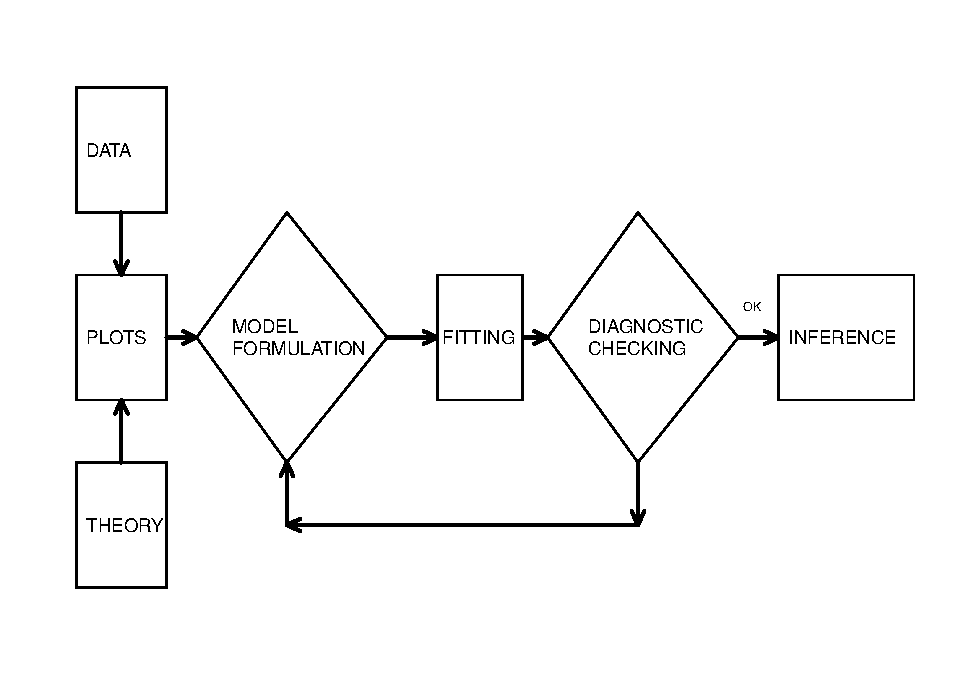
\includegraphics{RegressModelDataCamp_files/figure-latex/unnamed-chunk-138-1.pdf}

Show Overhead B Details. Many possible models

\hypertarget{toggleOver4.1B}{}
\[
\begin{array}{l|r}
\hline
\text{E }y = \beta _{0} &     \text{1 model with no variables }  \\
\text{E }y = \beta _{0}+\beta_1 x_{i}, &  \text{4 models with one variable}  \\
\text{E }y = \beta _{0}+\beta_1 x_{i}+\beta_{2} x_{j}, &  \text{6 models with two variables}  \\
\text{E }y = \beta _{0}+\beta_{1} x_{1}+\beta_{2} x_{j} +\beta_{3} x_{k},&  \text{4 models with three variables} \\
\text{E }y = \beta_{0} + \beta_{1} x_{1} + \beta_{2} x_{2} +\beta_{3} x_{3}+\beta_{4} x_{4} &  \text{1 model with all variables}  \\ 
\hline
\end{array}
\]

\begin{itemize}
\tightlist
\item
  With \emph{k} explanatory variables, there are \(2^k\) possible linear
  models
\item
  There are infinitely many nonlinear ones!!
\end{itemize}

Show Overhead C Details. Model validation

\hypertarget{toggleOver4.1C}{}
\begin{itemize}
\tightlist
\item
  Model validation is the process of confirming our proposed model.
\item
  Concern: \emph{data-snooping} - fitting many models to a single set of
  data.

  \begin{itemize}
  \tightlist
  \item
    Response to concern: \emph{out-of-sample validation}.
  \item
    Divide the data into \emph{model development}, or \emph{training}
    and \emph{validation}, or \emph{test}, subsamples.
  \end{itemize}
\end{itemize}

\begin{Shaded}
\begin{Highlighting}[]
\KeywordTok{par}\NormalTok{(}\DataTypeTok{mai=}\KeywordTok{c}\NormalTok{(}\DecValTok{0}\NormalTok{,}\FloatTok{0.1}\NormalTok{,}\DecValTok{0}\NormalTok{,}\DecValTok{0}\NormalTok{))}
\KeywordTok{plot.new}\NormalTok{()}
\KeywordTok{plot.window}\NormalTok{(}\DataTypeTok{xlim=}\KeywordTok{c}\NormalTok{(}\DecValTok{0}\NormalTok{,}\DecValTok{18}\NormalTok{),}\DataTypeTok{ylim=}\KeywordTok{c}\NormalTok{(}\OperatorTok{-}\DecValTok{10}\NormalTok{,}\DecValTok{10}\NormalTok{))}
\KeywordTok{rect}\NormalTok{(}\DecValTok{1}\NormalTok{,}\OperatorTok{-}\FloatTok{1.2}\NormalTok{,}\DecValTok{14}\NormalTok{,}\FloatTok{1.2}\NormalTok{)}
\KeywordTok{rect}\NormalTok{(}\DecValTok{7}\NormalTok{,}\DecValTok{4}\NormalTok{,}\DecValTok{15}\NormalTok{,}\DecValTok{8}\NormalTok{)}
\KeywordTok{rect}\NormalTok{(}\DecValTok{1}\NormalTok{,}\OperatorTok{-}\DecValTok{8}\NormalTok{,}\DecValTok{6}\NormalTok{,}\OperatorTok{-}\DecValTok{4}\NormalTok{)}
\NormalTok{x<-}\KeywordTok{seq}\NormalTok{(}\FloatTok{1.5}\NormalTok{,}\DecValTok{9}\NormalTok{,}\DataTypeTok{length=}\DecValTok{6}\NormalTok{)}
\NormalTok{y<-}\KeywordTok{rep}\NormalTok{(}\DecValTok{0}\NormalTok{,}\DecValTok{6}\NormalTok{)}
\KeywordTok{text}\NormalTok{(x,y,}\DataTypeTok{labels=}\KeywordTok{c}\NormalTok{(}\DecValTok{1}\OperatorTok{:}\DecValTok{6}\NormalTok{),}\DataTypeTok{cex=}\FloatTok{1.5}\NormalTok{)}
\NormalTok{x1<-}\KeywordTok{seq}\NormalTok{(}\FloatTok{10.5}\NormalTok{,}\FloatTok{11.5}\NormalTok{,}\DataTypeTok{length=}\DecValTok{3}\NormalTok{)}
\NormalTok{y1<-}\KeywordTok{rep}\NormalTok{(}\DecValTok{0}\NormalTok{,}\DecValTok{3}\NormalTok{)}
\KeywordTok{text}\NormalTok{(x1,y1,}\DataTypeTok{labels=}\KeywordTok{rep}\NormalTok{(}\StringTok{"."}\NormalTok{,}\DecValTok{3}\NormalTok{),}\DataTypeTok{cex=}\DecValTok{3}\NormalTok{)}
\KeywordTok{text}\NormalTok{(}\DecValTok{13}\NormalTok{,}\DecValTok{0}\NormalTok{,}\DataTypeTok{labels=}\StringTok{"n"}\NormalTok{,}\DataTypeTok{cex=}\FloatTok{1.5}\NormalTok{)}

\KeywordTok{text}\NormalTok{(}\DecValTok{15}\NormalTok{,}\DecValTok{0}\NormalTok{,}\DataTypeTok{labels=}\StringTok{"ORIGINAL}\CharTok{\textbackslash{}n}\StringTok{SAMPLE}\CharTok{\textbackslash{}n}\StringTok{SIZE n"}\NormalTok{,}\DataTypeTok{adj=}\DecValTok{0}\NormalTok{)}
\KeywordTok{text}\NormalTok{(}\FloatTok{7.5}\NormalTok{,}\DecValTok{6}\NormalTok{,}\DataTypeTok{labels=}\StringTok{"MODEL DEVELOPMENT}\CharTok{\textbackslash{}n}\StringTok{SUBSAMPLE SIZE"}\NormalTok{,}\DataTypeTok{adj=}\DecValTok{0}\NormalTok{)}
\KeywordTok{text}\NormalTok{(}\FloatTok{12.5}\NormalTok{,}\FloatTok{5.3}\NormalTok{, }\KeywordTok{expression}\NormalTok{(n[}\DecValTok{1}\NormalTok{]), }\DataTypeTok{adj=}\DecValTok{0}\NormalTok{, }\DataTypeTok{cex=}\FloatTok{1.1}\NormalTok{)}
\KeywordTok{text}\NormalTok{(}\FloatTok{1.4}\NormalTok{,}\OperatorTok{-}\DecValTok{6}\NormalTok{,}\DataTypeTok{labels=}\StringTok{"VALIDATION}\CharTok{\textbackslash{}n}\StringTok{SUBSAMPLE}\CharTok{\textbackslash{}n}\StringTok{SIZE"}\NormalTok{,}\DataTypeTok{adj=}\DecValTok{0}\NormalTok{)}
\KeywordTok{text}\NormalTok{(}\FloatTok{2.8}\NormalTok{,}\OperatorTok{-}\FloatTok{7.2}\NormalTok{,}\KeywordTok{expression}\NormalTok{(n[}\DecValTok{2}\NormalTok{]),}\DataTypeTok{adj=}\DecValTok{0}\NormalTok{, }\DataTypeTok{cex=}\FloatTok{1.1}\NormalTok{)}

\KeywordTok{arrows}\NormalTok{(}\FloatTok{1.8}\NormalTok{,}\FloatTok{0.8}\NormalTok{,}\FloatTok{8.3}\NormalTok{,}\FloatTok{3.9}\NormalTok{,}\DataTypeTok{code=}\DecValTok{2}\NormalTok{,}\DataTypeTok{lwd=}\DecValTok{2}\NormalTok{,}\DataTypeTok{angle=}\DecValTok{15}\NormalTok{,}\DataTypeTok{length=}\FloatTok{0.2}\NormalTok{)}
\KeywordTok{arrows}\NormalTok{(}\FloatTok{4.8}\NormalTok{,}\FloatTok{0.8}\NormalTok{,}\DecValTok{9}\NormalTok{,}\FloatTok{3.8}\NormalTok{,}\DataTypeTok{code=}\DecValTok{2}\NormalTok{,}\DataTypeTok{lwd=}\DecValTok{2}\NormalTok{,}\DataTypeTok{angle=}\DecValTok{15}\NormalTok{,}\DataTypeTok{length=}\FloatTok{0.2}\NormalTok{)}
\KeywordTok{arrows}\NormalTok{(}\FloatTok{9.1}\NormalTok{,}\FloatTok{0.9}\NormalTok{,}\FloatTok{9.5}\NormalTok{,}\FloatTok{3.8}\NormalTok{,}\DataTypeTok{code=}\DecValTok{2}\NormalTok{,}\DataTypeTok{lwd=}\DecValTok{2}\NormalTok{,}\DataTypeTok{angle=}\DecValTok{15}\NormalTok{,}\DataTypeTok{length=}\FloatTok{0.2}\NormalTok{)}
\KeywordTok{arrows}\NormalTok{(}\FloatTok{12.8}\NormalTok{,}\FloatTok{0.8}\NormalTok{,}\DecValTok{10}\NormalTok{,}\FloatTok{3.8}\NormalTok{,}\DataTypeTok{code=}\DecValTok{2}\NormalTok{,}\DataTypeTok{lwd=}\DecValTok{2}\NormalTok{,}\DataTypeTok{angle=}\DecValTok{15}\NormalTok{,}\DataTypeTok{length=}\FloatTok{0.2}\NormalTok{)}
\KeywordTok{arrows}\NormalTok{(}\FloatTok{2.9}\NormalTok{,}\OperatorTok{-}\FloatTok{0.9}\NormalTok{,}\FloatTok{2.5}\NormalTok{,}\OperatorTok{-}\FloatTok{3.8}\NormalTok{,}\DataTypeTok{code=}\DecValTok{2}\NormalTok{,}\DataTypeTok{lwd=}\DecValTok{2}\NormalTok{,}\DataTypeTok{angle=}\DecValTok{15}\NormalTok{,}\DataTypeTok{length=}\FloatTok{0.2}\NormalTok{)}
\KeywordTok{arrows}\NormalTok{(}\FloatTok{5.9}\NormalTok{,}\OperatorTok{-}\FloatTok{0.9}\NormalTok{,}\FloatTok{3.1}\NormalTok{,}\OperatorTok{-}\FloatTok{3.8}\NormalTok{,}\DataTypeTok{code=}\DecValTok{2}\NormalTok{,}\DataTypeTok{lwd=}\DecValTok{2}\NormalTok{,}\DataTypeTok{angle=}\DecValTok{15}\NormalTok{,}\DataTypeTok{length=}\FloatTok{0.2}\NormalTok{)}
\KeywordTok{arrows}\NormalTok{(}\FloatTok{7.4}\NormalTok{,}\OperatorTok{-}\FloatTok{0.9}\NormalTok{,}\FloatTok{3.5}\NormalTok{,}\OperatorTok{-}\FloatTok{3.8}\NormalTok{,}\DataTypeTok{code=}\DecValTok{2}\NormalTok{,}\DataTypeTok{lwd=}\DecValTok{2}\NormalTok{,}\DataTypeTok{angle=}\DecValTok{15}\NormalTok{,}\DataTypeTok{length=}\FloatTok{0.2}\NormalTok{)}
\end{Highlighting}
\end{Shaded}

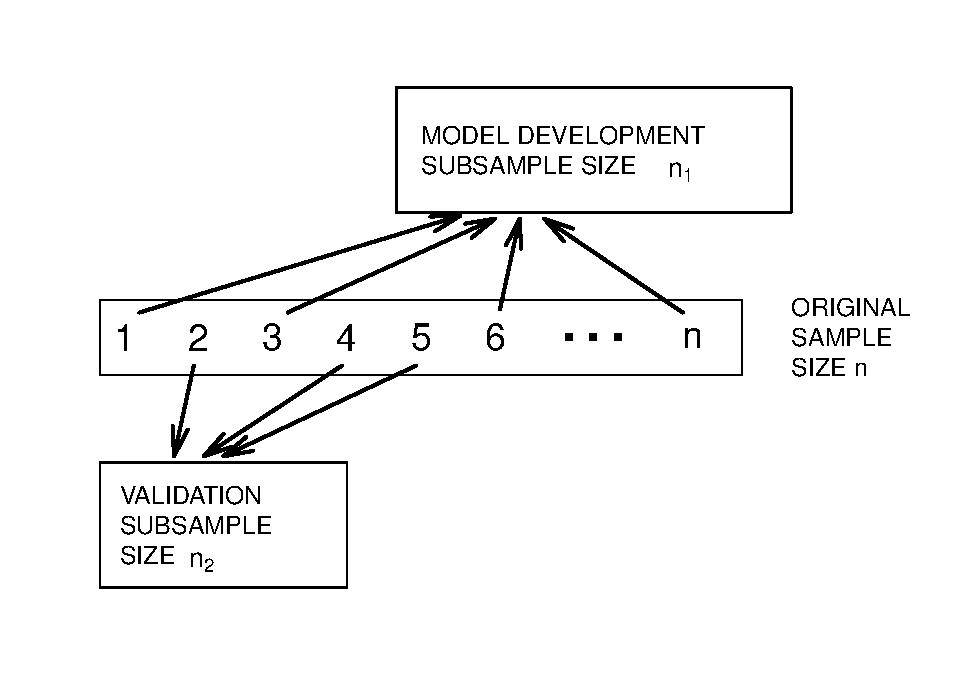
\includegraphics{RegressModelDataCamp_files/figure-latex/unnamed-chunk-139-1.pdf}

\subsection{MC Exercise. An iterative approach to data
modeling}\label{mc-exercise.-an-iterative-approach-to-data-modeling}

Which of the following is not true?

\begin{itemize}
\tightlist
\item
  A. Diagnostic checking reveals symptoms of mistakes made in previous
  specifications.
\item
  B. Diagnostic checking provides ways to correct mistakes made in
  previous specifications.
\item
  C. Model formulation is accomplished by using prior knowledge of
  relationships.
\item
  D. Understanding theoretical model properties is not really helpful
  when matching a model to data or inferring general relationships based
  on the data.
\end{itemize}

\section{Automatic variable selection
procedures}\label{automatic-variable-selection-procedures}

\begin{center}\rule{0.5\linewidth}{\linethickness}\end{center}

In this section, you learn how to:

\begin{itemize}
\tightlist
\item
  Identify some examples of automatic variable selection procedures
\item
  Describe the purpose of automatic variable selection procedures and
  their limitations
\item
  Describe ``data-snooping''
\end{itemize}

\begin{center}\rule{0.5\linewidth}{\linethickness}\end{center}

\subsection{Video}\label{video-15}

\subsubsection*{Video Overhead Details}\label{video-overhead-details-15}
\addcontentsline{toc}{subsubsection}{Video Overhead Details}

Show Overhead A Details. Classic stepwise regression algorithm

\hypertarget{toggleOver4.2A}{}
Suppose that the analyst has identified one variable as the outcome,
\(y\), and \(k\) potential explanatory variables,
\(x_1, x_2, \ldots, x_k\).

\begin{itemize}
\tightlist
\item
  (i). Consider all possible regressions using one explanatory variable.
  Choose the one with the highest \emph{t}-statistic.
\item
  (ii). Add a variable to the model from the previous step. The variable
  to enter is with the highest \emph{t}-statistic.
\item
  (iii). Delete a variable to the model from the previous step. Delete
  the variable with the small \emph{t}-statistic if the statistic is
  less than, e.g., 2 in absolute value.
\item
  (iv). Repeat steps (ii) and (iii) until all possible additions and
  deletions are performed.
\end{itemize}

Show Overhead B Details. Drawbacks of stepwise regression

\hypertarget{toggleOver4.2B}{}
\begin{itemize}
\tightlist
\item
  The procedure ``snoops'' through a large number of models and may fit
  the data ``too well.''
\item
  There is no guarantee that the selected model is the best.

  \begin{itemize}
  \tightlist
  \item
    The algorithm does not consider models that are based on nonlinear
    combinations of explanatory variables.
  \item
    It ignores the presence of outliers and high leverage points.
  \end{itemize}
\end{itemize}

Show Overhead C Details. Data-snooping in stepwise regression

\hypertarget{toggleOver4.2C}{}
\begin{itemize}
\tightlist
\item
  Generate \(y\) and \(x_1 - x_{50}\) using a random number generator
\item
  By design, there is no relation between \(y\) and \(x_1 - x_{50}\).
\item
  \textbf{But}, through stepwise regression, we \textbf{``discover''} a
  relationship that explains 14\% of the variation!!!
\end{itemize}

\begin{verbatim}
Call: lm(formula = y ~ xvar27 + xvar29 + xvar32, data = X)

Coefficients:
            Estimate Std. Error t value Pr(>|t|)  
(Intercept) -0.04885    0.09531  -0.513   0.6094  
xvar27        0.21063    0.09724   2.166   0.0328 *
xvar29        0.24887    0.10185   2.443   0.0164 *
xvar32        0.25390    0.09823   2.585   0.0112 *

Signif. codes:  0 '***' 0.001 '**' 0.01 '*' 0.05 '.' 0.1 ' ' 1

Residual standard error: 0.9171 on 96 degrees of freedom
Multiple R-squared:  0.1401,    Adjusted R-squared:  0.1132 
F-statistic: 5.212 on 3 and 96 DF,  p-value: 0.002233
\end{verbatim}

Show Overhead D Details. Variants of stepwise regression

\hypertarget{toggleOver4.2D}{}
This uses the \texttt{R} function
\href{https://www.rdocumentation.org/packages/stats/versions/3.5.0/topics/step}{step()}

\begin{itemize}
\tightlist
\item
  The option \texttt{direction} can be used to change how variables
  enter

  \begin{itemize}
  \tightlist
  \item
    Forward selection. Add one variable at a time without trying to
    delete variables.
  \item
    Backwards selection. Start with the full model and delete one
    variable at a time without trying to add variables.
  \end{itemize}
\item
  The option \texttt{scope} can be used to specify which variables must
  be included
\end{itemize}

Show Overhead E Details. Automatic variable selection procedures

\hypertarget{toggleOver4.2E}{}
\begin{itemize}
\tightlist
\item
  Stepwise regression is a type of automatic variable selection
  procedure.
\item
  These procedures are useful because they can quickly search through
  several candidate models. They mechanize certain routine tasks and are
  excellent at discovering patterns in data.
\item
  They are so good at detecting patterns that they analyst must be wary
  of overfitting (data-snooping)\\
\item
  They can miss certain patterns (nonlinearities, unusual points)
\item
  A model suggested by automatic variable selection procedures should be
  subject to the same careful diagnostic checking procedures as a model
  arrived at by any other means
\end{itemize}

\subsection{Exercise. Data-snooping in stepwise
regression}\label{exercise.-data-snooping-in-stepwise-regression}

\textbf{Assignment Text}

Automatic variable selection procedures, such as the classic stepwise
regression algorithm, are very good at detecting patterns. Sometimes
they are too good in the sense that they detect patterns in the sample
that are not evident in the population from which the data are drawn.
The detect ``spurious'' patterns.

This exercise illustrates this phenomenom by using a simulation,
designed so that the outcome variable (\emph{y}) and the explanatory
variables are mutually independent. So, by design, there is no
relationship between the outcome and the explanatory variables.

As part of the code set-up, we have \emph{n} = 100 observations
generated of the outcome \emph{y} and 50 explanatory variables,
\texttt{xvar1} through \texttt{xvar50}. As anticipated, collections of
explanatory variables are not statistically significant. However, with
the
\href{https://www.rdocumentation.org/packages/stats/versions/3.5.0/topics/step}{step()}
function, you will find some statistically significant relationships!

\textbf{Instructions}

\begin{itemize}
\tightlist
\item
  Fit a basic linear regression model and MLR model with the first ten
  explanatory variables. Compare the models via an \emph{F} test.
\item
  Fit a multiple linear regression model with all fifty explanatory
  variables. Compare this model to the one with ten variables via an
  \emph{F} test.
\item
  Use the \texttt{step} function to find the best model starting with
  the fitted model containing all fifty explanatory variables and
  summarize the fit.
\end{itemize}

\textbf{Hint.} The code shows stepwise regression using BIC, a criterion
that results in simpler models than AIC. For AIC, use the option
\texttt{k=2} in the {[}step(){]} function (the default)

eyJsYW5ndWFnZSI6InIiLCJwcmVfZXhlcmNpc2VfY29kZSI6InNldC5zZWVkKDEyMzcpXG5YIDwtIGFzLmRhdGEuZnJhbWUobWF0cml4KHJub3JtKDEwMCo1MCwgbWVhbiA9IDAsIHNkID0gMSksIG5jb2wgPSA1MCkpXG5jb2xuYW1lcyhYKSA8LSBwYXN0ZShcInh2YXJcIiwgMTo1MCwgc2VwID0gXCJcIilcblgkeSA8LSB3aXRoKFgsIG1hdHJpeChybm9ybSgxMDAqMSwgbWVhbiA9IDAsIHNkID0gMSksIG5jb2wgPSAxKSlcbiNjb3IoWFssYyhcInh2YXIxXCIsXCJ4dmFyMlwiLFwieHZhcjNcIixcInh2YXI0XCIsXCJ4dmFyNVwiLFwieHZhcjZcIixcInh2YXI3XCIsXCJ4dmFyOFwiLFwieHZhcjlcIixcInh2YXIxMFwiLFwieVwiKV0sIHVzZSA9IFwiY29tcGxldGUub2JzXCIpIiwic2FtcGxlIjoiIyBGaXQgYSBiYXNpYyBsaW5lYXIgcmVncmVzc2lvbiBtb2RlbCBhbmQgTUxSIG1vZGVsIHdpdGggdGhlIGZpcnN0IHRlbiBleHBsYW5hdG9yeSB2YXJpYWJsZXMuIENvbXBhcmUgdGhlIG1vZGVscyB2aWEgYW4gKkYqIHRlc3QuXG5tb2RlbF9zdGVwMSA8LSBsbSh5IH4geHZhcjEsIGRhdGEgPSBYKVxubW9kZWxfc3RlcDEwIDwtIGxtKHkgfiB4dmFyMSArIHh2YXIyICsgeHZhcjMgKyB4dmFyNCArIHh2YXI1ICsgeHZhcjYgKyB4dmFyNyArIHh2YXI4ICsgeHZhcjkgKyB4dmFyMTAsIGRhdGEgPSBYKVxuYW5vdmEoX19fLCBfX18pXG5cbiMgRml0IGEgbXVsdGlwbGUgbGluZWFyIHJlZ3Jlc3Npb24gbW9kZWwgd2l0aCBhbGwgZmlmdHkgZXhwbGFuYXRvcnkgdmFyaWFibGVzLiBDb21wYXJlIHRoaXMgbW9kZWwgdG8gdGhlIG9uZSB3aXRoIHRlbiB2YXJpYWJsZXMgdmlhIGFuICpGKiB0ZXN0LlxubW9kZWxfc3RlcDUwIDwtIGxtKHkgfiB4dmFyMSArIHh2YXIyICsgeHZhcjMgKyB4dmFyNCArIHh2YXI1ICsgeHZhcjYgKyB4dmFyNyArIHh2YXI4ICsgeHZhcjkgKyB4dmFyMTAgKyB4dmFyMTEgKyB4dmFyMTIgKyB4dmFyMTMgKyB4dmFyMTQgKyB4dmFyMTUgKyB4dmFyMTYgKyB4dmFyMTcgKyB4dmFyMTggKyB4dmFyMTkgKyB4dmFyMjAgKyB4dmFyMjEgKyB4dmFyMjIgKyB4dmFyMjMgKyB4dmFyMjQgKyB4dmFyMjUgKyB4dmFyMjYgKyB4dmFyMjcgKyB4dmFyMjggKyB4dmFyMjkgKyB4dmFyMzAgKyB4dmFyMzEgKyB4dmFyMzIgKyB4dmFyMzMgKyB4dmFyMzQgKyB4dmFyMzUgKyB4dmFyMzYgKyB4dmFyMzcgKyB4dmFyMzggKyB4dmFyMzkgKyB4dmFyNDAgKyB4dmFyNDEgKyB4dmFyNDIgKyB4dmFyNDMgKyB4dmFyNDQgKyB4dmFyNDUgKyB4dmFyNDYgKyB4dmFyNDcgKyB4dmFyNDggKyB4dmFyNDkgKyB4dmFyNTAsIGRhdGEgPSBYKVxuYW5vdmEoX19fLCBfX18pXG5cbiMgVXNlIHRoZSBgc3RlcGAgZnVuY3Rpb24sIHN0YXJ0aW5nIHdpdGggdGhlIGZpdHRlZCBtb2RlbCBjb250YWluaW5nIGFsbCBmaWZ0eSBleHBsYW5hdG9yeSB2YXJpYWJsZXMgYW5kIHN1bW1hcml6ZSB0aGUgZml0LlxuI0ZvciBCSUM6IFxubW9kZWxfc3RlcHdpc2UgPC0gc3RlcChfX18sIGRhdGEgPSBYLCBkaXJlY3Rpb249IFwiYm90aFwiLCBrID0gbG9nKG5yb3coWCkpLCB0cmFjZSA9IDApIFxuc3VtbWFyeShtb2RlbF9zdGVwd2lzZSkiLCJzb2x1dGlvbiI6Im1vZGVsX3N0ZXAxIDwtIGxtKHkgfiB4dmFyMSwgZGF0YSA9IFgpXG5tb2RlbF9zdGVwMTAgPC0gbG0oeSB+IHh2YXIxICsgeHZhcjIgKyB4dmFyMyArIHh2YXI0ICsgeHZhcjUgKyB4dmFyNiArIHh2YXI3ICsgeHZhcjggKyB4dmFyOSArIHh2YXIxMCwgZGF0YSA9IFgpXG5hbm92YShtb2RlbF9zdGVwMSxtb2RlbF9zdGVwMTApXG5tb2RlbF9zdGVwNTAgPC0gbG0oeSB+IHh2YXIxICsgeHZhcjIgKyB4dmFyMyArIHh2YXI0ICsgeHZhcjUgKyB4dmFyNiArIHh2YXI3ICsgeHZhcjggKyB4dmFyOSArIHh2YXIxMCArIHh2YXIxMSArIHh2YXIxMiArIHh2YXIxMyArIHh2YXIxNCArIHh2YXIxNSArIHh2YXIxNiArIHh2YXIxNyArIHh2YXIxOCArIHh2YXIxOSArIHh2YXIyMCArIHh2YXIyMSArIHh2YXIyMiArIHh2YXIyMyArIHh2YXIyNCArIHh2YXIyNSArIHh2YXIyNiArIHh2YXIyNyArIHh2YXIyOCArIHh2YXIyOSArIHh2YXIzMCArIHh2YXIzMSArIHh2YXIzMiArIHh2YXIzMyArIHh2YXIzNCArIHh2YXIzNSArIHh2YXIzNiArIHh2YXIzNyArIHh2YXIzOCArIHh2YXIzOSArIHh2YXI0MCArIHh2YXI0MSArIHh2YXI0MiArIHh2YXI0MyArIHh2YXI0NCArIHh2YXI0NSArIHh2YXI0NiArIHh2YXI0NyArIHh2YXI0OCArIHh2YXI0OSArIHh2YXI1MCwgZGF0YSA9IFgpXG5hbm92YShtb2RlbF9zdGVwMTAsbW9kZWxfc3RlcDUwKVxuXG4jRm9yIEJJQzogXG5tb2RlbF9zdGVwd2lzZSA8LSBzdGVwKG1vZGVsX3N0ZXA1MCwgZGF0YSA9IFgsIGRpcmVjdGlvbj0gXCJib3RoXCIsIGsgPSBsb2cobnJvdyhYKSksIHRyYWNlID0gMCkgXG5zdW1tYXJ5KG1vZGVsX3N0ZXB3aXNlKVxuXG4jIEFuIGV4YW1wbGUgd2l0aCBzY29wZVxuI21vZGVsX3N0ZXA1YSA8LSBzdGVwKG1vZGVsX3N0ZXA0LCBkYXRhID0gWCwgZGlyZWN0aW9uPSBcImJvdGhcIiwgaz1sb2cobnJvdyhYKSksIHRyYWNlID0gMCxcbiAgICAjICAgICAgICAgICAgc2NvcGUgPSBsaXN0KGxvd2VyID0gfnh2YXIxK3h2YXIyLCB1cHBlciA9IG1vZGVsX3N0ZXA0KSkgXG4jc3VtbWFyeShtb2RlbF9zdGVwNWEpXG4jRm9yIEFJQzogXG4jc3RlcChtb2RlbF9zdGVwNCwgZGF0YSA9IFgsIGRpcmVjdGlvbj0gXCJib3RoXCIsIGs9MiwgdHJhY2UgPSAwKSAjIGs9MiBpcyBieSBkZWZhdWx0ICIsInNjdCI6ImV4KCkgJT4lIGNoZWNrX29iamVjdChcIm1vZGVsX3N0ZXAxXCIpICU+JSBjaGVja19lcXVhbCgpXG5leCgpICU+JSBjaGVja19vYmplY3QoXCJtb2RlbF9zdGVwMTBcIikgJT4lIGNoZWNrX2VxdWFsKClcbmV4KCkgJT4lIGNoZWNrX2Z1bmN0aW9uKFwiYW5vdmFcIixpbmRleD0xKSAlPiUgY2hlY2tfcmVzdWx0KCkgJT4lIGNoZWNrX2VxdWFsKClcbmV4KCkgJT4lIGNoZWNrX29iamVjdChcIm1vZGVsX3N0ZXA1MFwiKSAlPiUgY2hlY2tfZXF1YWwoKVxuZXgoKSAlPiUgY2hlY2tfZnVuY3Rpb24oXCJhbm92YVwiLGluZGV4PTIpICU+JSBjaGVja19yZXN1bHQoKSAlPiUgY2hlY2tfZXF1YWwoKVxuZXgoKSAlPiUgY2hlY2tfb2JqZWN0KFwibW9kZWxfc3RlcHdpc2VcIikgJT4lIGNoZWNrX2VxdWFsKClcbmV4KCkgJT4lIGNoZWNrX2Z1bmN0aW9uKFwic3VtbWFyeVwiKSAlPiUgY2hlY2tfYXJnKC4sIFwib2JqZWN0XCIpICU+JSBjaGVja19lcXVhbCgpXG5zdWNjZXNzX21zZyhcIkV4Y2VsbGVudCEgVGhlIHN0ZXAgcHJvY2VkdXJlIHJlcGVhdGVkbHkgZml0cyBtYW55IG1vZGVscyB0byBhIGRhdGEgc2V0LiBXZSBzdW1tYXJpemUgZWFjaCBmaXQgd2l0aCBoeXBvdGhlc2lzIHRlc3Rpbmcgc3RhdGlzdGljcyBsaWtlIHQtc3RhdGlzdGljcyBhbmQgcC12YWx1ZXMuIEJ1dCwgcmVtZW1iZXIgdGhhdCBoeXBvdGhlc2lzIHRlc3RzIGFyZSBkZXNpZ25lZCB0byBmYWxzZWx5IGRldGVjdCBhIHJlbGF0aW9uc2hpcCBhIGZyYWN0aW9uIG9mIHRoZSB0aW1lICh0eXBpY2FsbHkgNSUpLiBGb3IgZXhhbXBsZSwgaWYgeW91IHJ1biBhIHQtdGVzdCA1MCB0aW1lcyAoZm9yIGVhY2ggZXhwbGFuYXRvcnkgdmFyaWFibGUpLCB5b3UgY2FuIGV4cGVjdCB0byBnZXQgdHdvIG9yIHRocmVlIHN0YXRpc3RpY2FsbHkgc2lnbmlmaWNhbnQgZXhwbGFuYXRvcnkgdmFyaWFibGVzIGV2ZW4gZm9yIHVucmVsYXRlZCB2YXJpYWJsZXMgKGJlY2F1c2UgNTAgdGltZXMgMC4wNSA9IDIuNSkuXCIpIn0=

\section{Residual analysis}\label{residual-analysis}

\begin{center}\rule{0.5\linewidth}{\linethickness}\end{center}

In this section, you learn how to:

\begin{itemize}
\tightlist
\item
  Explain how residual analysis can be used to improve a model
  specification
\item
  Use relationships between residuals and potential explanatory
  variables to improve model specification
\end{itemize}

\begin{center}\rule{0.5\linewidth}{\linethickness}\end{center}

\subsection{Video}\label{video-16}

\subsubsection*{Video Overhead Details}\label{video-overhead-details-16}
\addcontentsline{toc}{subsubsection}{Video Overhead Details}

Show Overhead A Details. Residual analysis

\hypertarget{toggleOver4.3A}{}
\begin{itemize}
\tightlist
\item
  Use \(e_i = y_i - \hat{y}_i\) as the \emph{i}th residual.
\item
  Later, I will discuss rescaling by, for example, \(s\), to get a
  standardized residual.
\item
  \emph{Role of residuals}: If the model formulation is correct, then
  residuals should be approximately equal to random errors or ``white
  noise.''
\item
  \emph{Method of attack}: Look for patterns in the residuals. Use this
  information to improve the model specification.
\end{itemize}

Show Overhead B Details. Using residuals to select explanatory variables

\hypertarget{toggleOver4.3B}{}
\begin{itemize}
\tightlist
\item
  Residual analysis can help identify additional explanatory variables
  that may be used to improve the formulation of the model.
\item
  If the model is correct, then residuals should resemble random errors
  and contain no discernible patterns.
\item
  Thus, when comparing residuals to explanatory variables, we do not
  expect any relationships.
\item
  If we do detect a relationship, then this suggests the need to control
  for this additional variable.
\end{itemize}

Show Overhead C Details. Detecting relationships between residuals and
explanatory variables

\hypertarget{toggleOver4.3C}{}
\begin{itemize}
\tightlist
\item
  Calculate summary statistics and display the distribution of residuals
  to identify outliers.
\item
  Calculate the correlation between the residuals and additional
  explanatory variables to search for linear relationships.
\item
  Create scatter plots between the residuals and additional explanatory
  variables to search for nonlinear relationships.
\end{itemize}

\subsection{Exercise. Residual analysis and risk manager
survey}\label{exercise.-residual-analysis-and-risk-manager-survey}

\textbf{Assignment Text}

This exercise examines data, pre-loaded in the dataframe
\texttt{survey}, from a survey on the cost effectiveness of risk
management practices. Risk management practices are activities
undertaken by a firm to minimize the potential cost of future losses,
such as the event of a fire in a warehouse or an accident that injures
employees. This exercise develops a model that can be used to make
statements about cost of managing risks.

A measure of risk management cost effectiveness, \texttt{logcost}, is
the outcome variable. This variable is defined as total property and
casualty premiums and uninsured losses as a proportion of total assets,
in logarithmic units. It is a proxy for annual expenditures associated
with insurable events, standardized by company size. Explanatory
variables include \texttt{logsize}, the logarithm of total firm assets,
and \texttt{indcost}, a measure of the firm's industry risk.

\textbf{Instructions}

\begin{itemize}
\tightlist
\item
  Fit and summarize a MLR model using \texttt{logcost} as the outcome
  variable and \texttt{logsize} and \texttt{indcost} as explanatory
  variables.
\item
  Plot residuals of the fitted model versus \texttt{indcost} and
  superimpose a locally fitted line using the \texttt{R} function
  \href{https://www.rdocumentation.org/packages/stats/versions/3.5.0/topics/lowess}{lowess()}.
\item
  Fit and summarize a MLR model of \texttt{logcost} on \texttt{logsize},
  \texttt{indcost} and a squared version of \texttt{indcost}.
\item
  Plot residuals of the fitted model versus `indcost' and superimpose a
  locally fitted line using
  \href{https://www.rdocumentation.org/packages/stats/versions/3.5.0/topics/lowess}{lowess()}.
\end{itemize}

\textbf{Hint.} You can access model residuals using
\texttt{mlr.survey1\$residuals} or \texttt{mlr.survey1(\$residuals)}

eyJsYW5ndWFnZSI6InIiLCJwcmVfZXhlcmNpc2VfY29kZSI6IiNzdXJ2ZXkgPC0gcmVhZC5jc3YoXCJDU1ZEYXRhXFxcXFJpc2tfc3VydmV5LmNzdlwiLCBoZWFkZXI9VFJVRSlcbnN1cnZleSA8LSByZWFkLmNzdihcImh0dHBzOi8vYXNzZXRzLmRhdGFjYW1wLmNvbS9wcm9kdWN0aW9uL3JlcG9zaXRvcmllcy8yNjEwL2RhdGFzZXRzL2RjMWM1YmNlNDNlZjA3NmFhNzcxNjlhMjQyMTE4ZTJlNThkMDFmODIvUmlza19zdXJ2ZXkuY3N2XCIsIGhlYWRlcj1UUlVFKVxuc3VydmV5JGxvZ2Nvc3QgPC0gbG9nKHN1cnZleSRmaXJtY29zdClcbiNzdHIoc3VydmV5KSIsInNhbXBsZSI6IiMgUmVncmVzcyBgbG9nY29zdGAgb24gYGxvZ3NpemVgIGFuZCBgaW5kY29zdGAgXG5tbHIuc3VydmV5MSA8LSBsbShsb2djb3N0IH4gbG9nc2l6ZSArIGluZGNvc3QsIGRhdGEgPSBzdXJ2ZXkpXG5zdW1tYXJ5KF9fXylcblxuIyBQbG90IHJlc2lkdWFscyBvZiB0aGUgZml0dGVkIG1vZGVsIHZlcnN1cyBgaW5kY29zdGAgYW5kIHN1cGVyaW1wb3NlIGEgbG9jYWxseSBmaXR0ZWQgbGluZSB1c2luZyB0aGUgIGZ1bmN0aW9uIFtsb3dlc3MoKV1cbnBsb3Qoc3VydmV5JGluZGNvc3QsICBfX18pXG5saW5lcyhsb3dlc3Moc3VydmV5JGluZGNvc3QsIF9fXykpXG5cbiMgUmVncmVzcyBgbG9nY29zdGAgb24gYGxvZ3NpemVgIGFuZCBgaW5kY29zdGAgYW5kIGBpbmRjb3N0YCBzcXVhcmVkXG5tbHIuc3VydmV5MiA8LSBsbShfX18gfiBsb2dzaXplICsgcG9seShpbmRjb3N0LDIpLCBkYXRhID0gc3VydmV5KVxuc3VtbWFyeShfX18pXG5cbiMgUGxvdCByZXNpZHVhbHMgb2YgdGhpcyBmaXR0ZWQgbW9kZWwgYW5kIHN1cGVyaW1wb3NlIGEgbG9jYWxseSBmaXR0ZWQgbGluZSB1c2luZyB0aGUgZnVuY3Rpb24gW2xvd2VzcygpXVxucGxvdChzdXJ2ZXkkaW5kY29zdCwgX19fKVxubGluZXMobG93ZXNzKHN1cnZleSRpbmRjb3N0LCBfX18pKSIsInNvbHV0aW9uIjoibWxyLnN1cnZleTEgPC0gbG0obG9nY29zdCB+IGxvZ3NpemUgKyBpbmRjb3N0LCBkYXRhID0gc3VydmV5KVxuc3VtbWFyeShtbHIuc3VydmV5MSlcblxucGxvdChzdXJ2ZXkkaW5kY29zdCwgbWxyLnN1cnZleTEkcmVzaWR1YWxzKVxubGluZXMobG93ZXNzKHN1cnZleSRpbmRjb3N0LG1sci5zdXJ2ZXkxJHJlc2lkdWFscykpXG5cbm1sci5zdXJ2ZXkyIDwtIGxtKGxvZ2Nvc3QgfiBsb2dzaXplICsgcG9seShpbmRjb3N0LDIpLCBkYXRhID0gc3VydmV5KVxuc3VtbWFyeShtbHIuc3VydmV5MilcblxucGxvdChzdXJ2ZXkkaW5kY29zdCwgbWxyLnN1cnZleTIkcmVzaWR1YWxzKVxubGluZXMobG93ZXNzKHN1cnZleSRpbmRjb3N0LG1sci5zdXJ2ZXkyJHJlc2lkdWFscykpIiwic2N0IjoiZXgoKSAlPiUgY2hlY2tfb2JqZWN0KFwibWxyLnN1cnZleTFcIikgJT4lIGNoZWNrX2VxdWFsKClcbmV4KCkgJT4lIGNoZWNrX2Z1bmN0aW9uKFwic3VtbWFyeVwiLGluZGV4PTEpICU+JSBjaGVja19hcmcoLiwgXCJvYmplY3RcIikgJT4lIGNoZWNrX2VxdWFsKClcbmV4KCkgJT4lIGNoZWNrX2Z1bmN0aW9uKFwicGxvdFwiLGluZGV4PTEpICU+JXtcbiAgY2hlY2tfYXJnKC4sIFwieFwiKSAlPiUgY2hlY2tfZXF1YWwoKVxuICBjaGVja19hcmcoLiwgXCJ5XCIpICU+JSBjaGVja19lcXVhbCgpXG59XG5leCgpICU+JSBjaGVja19mdW5jdGlvbihcImxpbmVzXCIsaW5kZXg9MSlcbmV4KCkgJT4lIGNoZWNrX2Z1bmN0aW9uKFwibG93ZXNzXCIsaW5kZXg9MSkgJT4le1xuICBjaGVja19hcmcoLiwgXCJ4XCIpICU+JSBjaGVja19lcXVhbCgpXG4gIGNoZWNrX2FyZyguLCBcInlcIikgJT4lIGNoZWNrX2VxdWFsKClcbn1cbmV4KCkgJT4lIGNoZWNrX29iamVjdChcIm1sci5zdXJ2ZXkyXCIpICU+JSBjaGVja19lcXVhbCgpXG5leCgpICU+JSBjaGVja19mdW5jdGlvbihcInN1bW1hcnlcIixpbmRleD0yKSAlPiUgY2hlY2tfYXJnKC4sIFwib2JqZWN0XCIpICU+JSBjaGVja19lcXVhbCgpXG5leCgpICU+JSBjaGVja19mdW5jdGlvbihcInBsb3RcIixpbmRleD0yKSAlPiV7XG4gIGNoZWNrX2FyZyguLCBcInhcIikgJT4lIGNoZWNrX2VxdWFsKClcbiAgY2hlY2tfYXJnKC4sIFwieVwiKSAlPiUgY2hlY2tfZXF1YWwoKVxufVxuZXgoKSAlPiUgY2hlY2tfZnVuY3Rpb24oXCJsaW5lc1wiLGluZGV4PTIpXG5leCgpICU+JSBjaGVja19mdW5jdGlvbihcImxvd2Vzc1wiLGluZGV4PTIpICU+JXtcbiAgY2hlY2tfYXJnKC4sIFwieFwiKSAlPiUgY2hlY2tfZXF1YWwoKVxuICBjaGVja19hcmcoLiwgXCJ5XCIpICU+JSBjaGVja19lcXVhbCgpXG59XG5zdWNjZXNzX21zZyhcIkV4Y2VsbGVudCEgSW4gdGhpcyBleGVyY2lzZSwgeW91IGV4YW1pbmVkIHJlc2lkdWFscyBmcm9tIGEgcHJlbGltaW5hcnkgbW9kZWwgZml0IGFuZCBkZXRlY3RlZCBhIG1pbGQgcXVhZHJhdGljIHBhdHRlcm4gaW4gYSB2YXJpYWJsZS4gVGhpcyBzdWdnZXN0ZWQgZW50ZXJpbmcgdGhlIHNxdWFyZWQgdGVybSBvZiB0aGF0IHZhcmlhYmxlIGludG8gdGhlIG1vZGVsIHNwZWNpZmljYXRpb24uIFRoZSByZWZpdCBvZiB0aGlzIG5ldyBtb2RlbCBzdWdnZXN0cyB0aGF0IHRoZSBzcXVhcmVkIHRlcm0gaGFzIGltcG9ydGFudCBleHBsYW5hdG9yeSBpbmZvcm1hdGlvbi4gVGhlIHNxdWFyZWQgdGVybSBpcyBhIG5vbmxpbmVhciBhbHRlcm5hdGl2ZSB0aGF0IGlzIG5vdCBhdmFpbGFibGUgaW4gbWFueSBhdXRvbWF0aWMgdmFyaWFibGUgc2VsZWN0aW9uIHByb2NlZHVyZXMuXCIpIn0=

\subsection{Exercise. Added variable plot and refrigerator
prices}\label{exercise.-added-variable-plot-and-refrigerator-prices}

\textbf{Assignment Text}

What characteristics of a refrigerator are important in determining its
price (\texttt{price})? We consider here several characteristics of a
refrigerator, including the size of the refrigerator in cubic feet
(\texttt{rsize}), the size of the freezer compartment in cubic feet
(\texttt{fsize}), the average amount of money spent per year to operate
the refrigerator (\texttt{ecost}, for energy cost), the number of
shelves in the refrigerator and freezer doors (\texttt{shelves}), and
the number of features (\texttt{features}). The features variable
includes shelves for cans, see-through crispers, ice makers, egg racks
and so on.

Both consumers and manufacturers are interested in models of
refrigerator prices. Other things equal, consumers generally prefer
larger refrigerators with lower energy costs that have more features.
Due to forces of supply and demand, we would expect consumers to pay
more for these refrigerators. A larger refrigerator with lower energy
costs that has more features at the similar price is considered a
bargain to the consumer. How much extra would the consumer be willing to
pay for this additional space? A model of prices for refrigerators on
the market provides some insight to this question.

To this end, we analyze data from \emph{n} = 37 refrigerators.

\textbf{Instructions}

\begin{Shaded}
\begin{Highlighting}[]
\CommentTok{# Pre-exercise code}
\NormalTok{Refrig <-}\StringTok{ }\KeywordTok{read.table}\NormalTok{(}\StringTok{"CSVData}\CharTok{\textbackslash{}\textbackslash{}}\StringTok{Refrig.csv"}\NormalTok{, }\DataTypeTok{header =} \OtherTok{TRUE}\NormalTok{, }\DataTypeTok{sep =} \StringTok{","}\NormalTok{)}
\KeywordTok{summary}\NormalTok{(Refrig)}
\NormalTok{Refrig1 <-}\StringTok{ }\NormalTok{Refrig[}\KeywordTok{c}\NormalTok{(}\StringTok{"price"}\NormalTok{, }\StringTok{"ecost"}\NormalTok{, }\StringTok{"rsize"}\NormalTok{, }\StringTok{"fsize"}\NormalTok{, }\StringTok{"shelves"}\NormalTok{, }\StringTok{"s_sq_ft"}\NormalTok{, }\StringTok{"features"}\NormalTok{)]}
\KeywordTok{round}\NormalTok{(}\KeywordTok{cor}\NormalTok{(Refrig1), }\DataTypeTok{digits =} \DecValTok{3}\NormalTok{)}
\NormalTok{refrig_mlr1 <-}\StringTok{ }\KeywordTok{lm}\NormalTok{(price }\OperatorTok{~}\StringTok{ }\NormalTok{rsize }\OperatorTok{+}\StringTok{ }\NormalTok{fsize }\OperatorTok{+}\StringTok{ }\NormalTok{shelves }\OperatorTok{+}\StringTok{ }\NormalTok{features, }\DataTypeTok{data =}\NormalTok{ Refrig)}
\KeywordTok{summary}\NormalTok{(refrig_mlr1)}
\NormalTok{Refrig}\OperatorTok{$}\NormalTok{residuals1 <-}\StringTok{ }\KeywordTok{residuals}\NormalTok{(refrig_mlr1)}
\NormalTok{refrig_mlr2 <-}\StringTok{ }\KeywordTok{lm}\NormalTok{(ecost }\OperatorTok{~}\StringTok{ }\NormalTok{rsize }\OperatorTok{+}\StringTok{ }\NormalTok{fsize }\OperatorTok{+}\StringTok{ }\NormalTok{shelves }\OperatorTok{+}\StringTok{ }\NormalTok{features, }\DataTypeTok{data =}\NormalTok{ Refrig)}
\KeywordTok{summary}\NormalTok{(refrig_mlr2)}
\NormalTok{Refrig}\OperatorTok{$}\NormalTok{residuals2 <-}\StringTok{ }\KeywordTok{residuals}\NormalTok{(refrig_mlr2)}
\KeywordTok{plot}\NormalTok{(Refrig}\OperatorTok{$}\NormalTok{residuals2, Refrig}\OperatorTok{$}\NormalTok{residuals1)}
\end{Highlighting}
\end{Shaded}

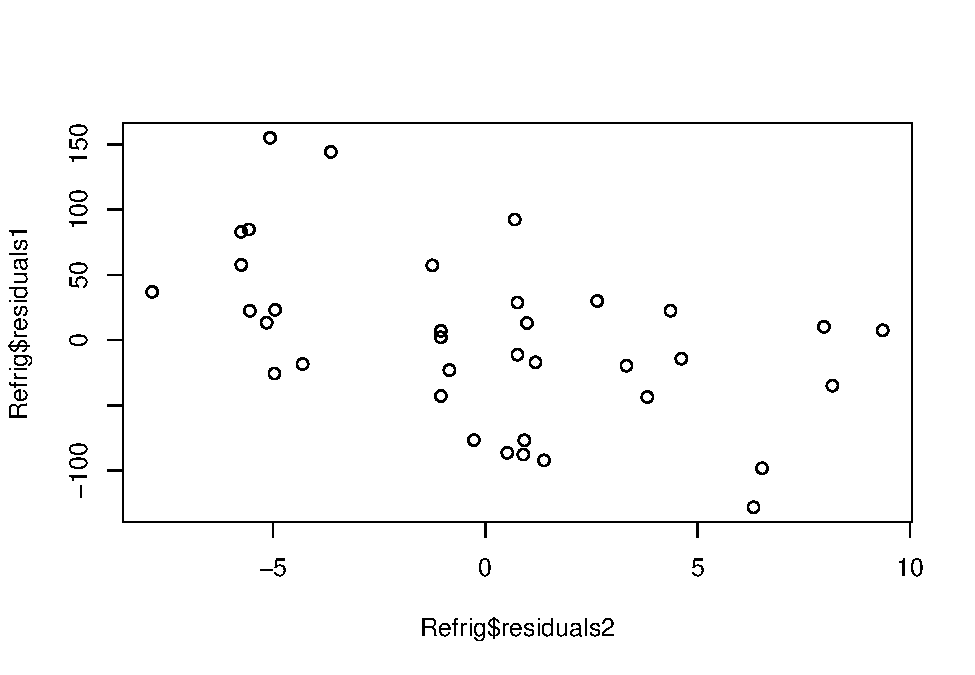
\includegraphics{RegressModelDataCamp_files/figure-latex/unnamed-chunk-148-1.pdf}

\begin{Shaded}
\begin{Highlighting}[]
\CommentTok{#library(Rcmdr)}
\CommentTok{#refrig_mlr3 <- lm(price ~ rsize + fsize + shelves + features + ecost, data = Refrig)}
\CommentTok{#avPlots(refrig_mlr3, terms = "ecost")}
\end{Highlighting}
\end{Shaded}

\begin{verbatim}
     price            ecost           rsize          fsize      
 Min.   : 460.0   Min.   :60.00   Min.   :12.6   Min.   :4.100  
 1st Qu.: 545.0   1st Qu.:66.00   1st Qu.:12.9   1st Qu.:4.400  
 Median : 590.0   Median :68.00   Median :13.2   Median :5.100  
 Mean   : 626.4   Mean   :70.51   Mean   :13.4   Mean   :5.184  
 3rd Qu.: 685.0   3rd Qu.:75.00   3rd Qu.:13.9   3rd Qu.:5.700  
 Max.   :1200.0   Max.   :94.00   Max.   :14.7   Max.   :7.400  
    shelves         s_sq_ft         features     
 Min.   :1.000   Min.   :20.60   Min.   : 1.000  
 1st Qu.:2.000   1st Qu.:23.40   1st Qu.: 2.000  
 Median :2.000   Median :24.00   Median : 3.000  
 Mean   :2.514   Mean   :24.53   Mean   : 3.459  
 3rd Qu.:3.000   3rd Qu.:25.50   3rd Qu.: 5.000  
 Max.   :5.000   Max.   :30.20   Max.   :12.000  
          price  ecost  rsize  fsize shelves s_sq_ft features
price     1.000  0.522 -0.024  0.720   0.400   0.155    0.697
ecost     0.522  1.000 -0.033  0.855   0.188   0.058    0.334
rsize    -0.024 -0.033  1.000 -0.235  -0.363   0.401   -0.096
fsize     0.720  0.855 -0.235  1.000   0.251   0.110    0.439
shelves   0.400  0.188 -0.363  0.251   1.000  -0.527    0.160
s_sq_ft   0.155  0.058  0.401  0.110  -0.527   1.000    0.083
features  0.697  0.334 -0.096  0.439   0.160   0.083    1.000

Call:
lm(formula = price ~ rsize + fsize + shelves + features, data = Refrig)

Residuals:
     Min       1Q   Median       3Q      Max 
-128.200  -34.963    7.081   28.716  155.096 

Coefficients:
            Estimate Std. Error t value Pr(>|t|)    
(Intercept)  -698.89     302.60  -2.310  0.02752 *  
rsize          56.50      20.56   2.748  0.00977 ** 
fsize          75.40      13.93   5.414 5.96e-06 ***
shelves        35.92      11.08   3.243  0.00277 ** 
features       25.16       5.04   4.992 2.04e-05 ***
---
Signif. codes:  0 '***' 0.001 '**' 0.01 '*' 0.05 '.' 0.1 ' ' 1

Residual standard error: 68.11 on 32 degrees of freedom
Multiple R-squared:  0.789, Adjusted R-squared:  0.7626 
F-statistic: 29.92 on 4 and 32 DF,  p-value: 2.102e-10


Call:
lm(formula = ecost ~ rsize + fsize + shelves + features, data = Refrig)

Residuals:
    Min      1Q  Median      3Q     Max 
-7.8483 -4.3064  0.5154  2.6324  9.3596 

Coefficients:
            Estimate Std. Error t value Pr(>|t|)    
(Intercept) -14.2165    20.9365  -0.679   0.5020    
rsize         2.8744     1.4225   2.021   0.0517 .  
fsize         8.9085     0.9636   9.245 1.49e-10 ***
shelves       0.2895     0.7664   0.378   0.7081    
features     -0.2006     0.3487  -0.575   0.5692    
---
Signif. codes:  0 '***' 0.001 '**' 0.01 '*' 0.05 '.' 0.1 ' ' 1

Residual standard error: 4.712 on 32 degrees of freedom
Multiple R-squared:  0.7637,    Adjusted R-squared:  0.7342 
F-statistic: 25.86 on 4 and 32 DF,  p-value: 1.247e-09
\end{verbatim}

\section{Unusual observations}\label{unusual-observations}

\begin{center}\rule{0.5\linewidth}{\linethickness}\end{center}

In this section, you learn how to:

\begin{itemize}
\tightlist
\item
  Compare and contrast three alternative definitions of a standardized
  residual
\item
  Evaluate three alternative options for dealing with outliers
\item
  Assess the impact of a high leverage observation
\item
  Evaluate options for dealing with high leverage observations
\item
  Describe the notion of influence and Cook's Distance for quantifying
  influence
\end{itemize}

\begin{center}\rule{0.5\linewidth}{\linethickness}\end{center}

\subsection{Video}\label{video-17}

\subsubsection*{Video Overhead Details}\label{video-overhead-details-17}
\addcontentsline{toc}{subsubsection}{Video Overhead Details}

Show Overhead A Details. Unusual observationsUnusual observations

\hypertarget{toggleOver4.4A}{}
\begin{itemize}
\tightlist
\item
  Regression coefficients can be expressed as (matrix) weighted averages
  of outcomes

  \begin{itemize}
  \tightlist
  \item
    Averages, even weighted averages can be strongly influenced by
    unusual observations
  \end{itemize}
\item
  Observations may be unusual in the \emph{y} direction or in the
  \emph{X} space
\item
  For unusual in the \emph{y} direction, we use a residual
  \(e = y - \hat{y}\)

  \begin{itemize}
  \tightlist
  \item
    By subtracting the fitted value \(\hat{y}\), we look to the \emph{y}
    distance from the regression plane
  \item
    In this way, we ``control'' for values of explanatory variables
  \end{itemize}
\end{itemize}

Show Overhead B Details. Standardized residuals

\hypertarget{toggleOver4.4B}{}
We standardize residuals so that we can focus on relationships of
interest and achieve carry-over of experience from one data set to
another.

Three commonly used definitions of standardize residuals are:

\[
\text{(a) }\frac{e_i}{s}, \ \ \ \text{ (b) }\frac{e_i}{s\sqrt{1-h_{ii}}}, \  \   \    
\text{(c)}\frac{e_i}{s_{(i)}\sqrt{1-h_{ii}}}.
\]

\begin{itemize}
\tightlist
\item
  First choice is simple
\item
  Second choice, from theory,
  \(\mathrm{Var}(e_i)=\sigma ^{2}(1-h_{ii}).\) Here, \(h_{ii}\) is the
  \(i\)th \emph{leverage} (defined later).
\item
  Third choice is termed ``studentized residuals''. Idea: numerator is
  independent of the denominator.
\end{itemize}

Show Overhead C Details. Outlier - an unusal standardized residual

\hypertarget{toggleOver4.4C}{}
\begin{itemize}
\tightlist
\item
  An \emph{outlier} is an observation that is not well fit by the model;
  these are observations where the residual is unusually large.
\item
  Unusual means what? Many packages mark a point if the
  \textbar{}standardized residual\textbar{} \textgreater{} 2.
\item
  Options for handling outliers

  \begin{itemize}
  \tightlist
  \item
    Ignore them in the analysis but be sure to discuss their effects.
  \item
    Delete them from the data set (but be sure to discuss their
    effects).
  \item
    Create a binary variable to indicator their presence. (This will
    increase your \(R^2\)!)
  \end{itemize}
\end{itemize}

Show Overhead D Details. High leverage points

\hypertarget{toggleOver4.4D}{}
\begin{itemize}
\tightlist
\item
  A high leverage point is an observation that is ``far away'' in the
  \(x\)-space from others.
\item
  One can get a feel for high leverage observations by looking a summary
  statistics (mins, maxs) for each explanatory variable.
\item
  Options for dealing with high leverage points are comparable to
  outliers, we can ignore their effects, delete them, or mark them with
  a binary indicator variable.
\end{itemize}

Show Overhead E Details. High leverage point graph

\hypertarget{toggleOver4.4E}{}
\begin{Shaded}
\begin{Highlighting}[]
\KeywordTok{library}\NormalTok{(cluster)}
\CommentTok{#library(MASS)}
\KeywordTok{par}\NormalTok{(}\DataTypeTok{mar=}\KeywordTok{c}\NormalTok{(}\FloatTok{3.2}\NormalTok{,}\FloatTok{5.4}\NormalTok{,.}\DecValTok{2}\NormalTok{,.}\DecValTok{2}\NormalTok{))}
\KeywordTok{plot}\NormalTok{(}\DecValTok{1}\NormalTok{,}\DecValTok{5}\NormalTok{,}\DataTypeTok{type=}\StringTok{"p"}\NormalTok{,}\DataTypeTok{pch=}\DecValTok{19}\NormalTok{,}\DataTypeTok{cex=}\FloatTok{1.5}\NormalTok{,}\DataTypeTok{xlab=}\StringTok{""}\NormalTok{,}\DataTypeTok{ylab=}\StringTok{""}\NormalTok{,}\DataTypeTok{cex.lab=}\FloatTok{1.5}\NormalTok{,}\DataTypeTok{xaxt=}\StringTok{"n"}\NormalTok{,}\DataTypeTok{yaxt=}\StringTok{"n"}\NormalTok{,}\DataTypeTok{xlim=}\KeywordTok{c}\NormalTok{(}\OperatorTok{-}\DecValTok{3}\NormalTok{,}\DecValTok{5}\NormalTok{),}\DataTypeTok{ylim=}\KeywordTok{c}\NormalTok{(}\OperatorTok{-}\DecValTok{12}\NormalTok{,}\DecValTok{12}\NormalTok{))}
\KeywordTok{mtext}\NormalTok{(}\KeywordTok{expression}\NormalTok{(x[}\DecValTok{2}\NormalTok{]), }\DataTypeTok{side=}\DecValTok{1}\NormalTok{,}\DataTypeTok{line=}\DecValTok{2}\NormalTok{, }\DataTypeTok{cex=}\FloatTok{2.0}\NormalTok{)}
\KeywordTok{mtext}\NormalTok{(}\KeywordTok{expression}\NormalTok{(x[}\DecValTok{1}\NormalTok{]), }\DataTypeTok{side=}\DecValTok{2}\NormalTok{, }\DataTypeTok{line=}\DecValTok{2}\NormalTok{, }\DataTypeTok{las=}\DecValTok{2}\NormalTok{, }\DataTypeTok{cex=}\FloatTok{2.0}\NormalTok{)}
\KeywordTok{arrows}\NormalTok{(}\FloatTok{1.5}\NormalTok{,}\DecValTok{5}\NormalTok{,}\DecValTok{4}\NormalTok{,}\DecValTok{5}\NormalTok{,}\DataTypeTok{code=}\DecValTok{1}\NormalTok{,}\DataTypeTok{lwd=}\DecValTok{2}\NormalTok{,}\DataTypeTok{angle=}\DecValTok{15}\NormalTok{,}\DataTypeTok{length=}\FloatTok{0.25}\NormalTok{)}
\NormalTok{xycov<-}\KeywordTok{matrix}\NormalTok{(}\KeywordTok{c}\NormalTok{(}\DecValTok{2}\NormalTok{, }\OperatorTok{-}\DecValTok{5}\NormalTok{,}\OperatorTok{-}\DecValTok{5}\NormalTok{, }\DecValTok{20}\NormalTok{),}\DataTypeTok{nrow=}\DecValTok{2}\NormalTok{,}\DataTypeTok{ncol=}\DecValTok{2}\NormalTok{)}
\NormalTok{xyloc<-}\KeywordTok{matrix}\NormalTok{(}\KeywordTok{c}\NormalTok{(}\DecValTok{0}\NormalTok{, }\DecValTok{0}\NormalTok{),}\DataTypeTok{nrow=}\DecValTok{1}\NormalTok{,}\DataTypeTok{ncol=}\DecValTok{2}\NormalTok{)}
\KeywordTok{polygon}\NormalTok{(}\KeywordTok{ellipsoidPoints}\NormalTok{(xycov, }\DataTypeTok{d2 =} \DecValTok{2}\NormalTok{, }\DataTypeTok{loc=}\NormalTok{xyloc),}\DataTypeTok{col=}\StringTok{"black"}\NormalTok{)}
\end{Highlighting}
\end{Shaded}

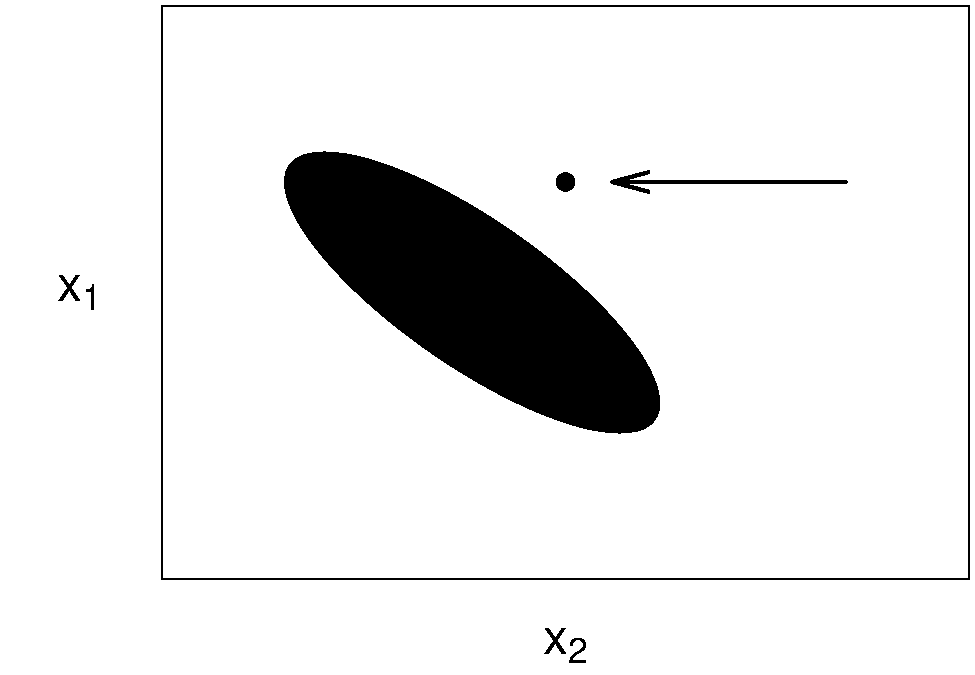
\includegraphics{RegressModelDataCamp_files/figure-latex/unnamed-chunk-149-1.pdf}

Show Overhead F Details. Leverage

\hypertarget{toggleOver4.4F}{}
\begin{itemize}
\tightlist
\item
  Using matrix algebra, one can express the \emph{i}th fitted value as a
  linear combination of observations
\end{itemize}

\[
\hat{y}_{i} = h_{i1} y_{1} + \cdots +h_{ii}y_{i}+\cdots+h_{in}y_{n}.
\]

\begin{itemize}
\tightlist
\item
  The term \(h_{ii}\) is known as the \emph{i}th leverage

  \begin{itemize}
  \tightlist
  \item
    The larger the value of \(h_{ii}\), the greater the effect of the
    \emph{i}th observation \(y_i\) on the \emph{i}th fitted value
    \(\hat{y}_i\).
  \item
    Statistical routines have values of the leverage coded, so computing
    this quantity. The key thing to know is that \(h_{ii}\) is based
    solely on the explanatory variables. If you change the \(y\) values,
    the leverage does not change.
  \item
    As a commonly used rule of thumb, a leverage is deemed to be
    ``unusual'' if its value exceeds three times the average (= number
    of regression coefficients divided by the number of observations.)
  \end{itemize}
\end{itemize}

\subsection{Exercise. Outlier example}\label{exercise.-outlier-example}

In chapter 2, we consider a fictitious data set of 19 ``base'' points
plus three different types of unusual points. In this exercise, we
consider the effect of one unusal point, ``C'', this both an outlier
(unusual in the ``y'' direction) and a high leverage point (usual in the
x-space). The data have been pre-loaded in the dataframe
\texttt{outlrC}.

\textbf{Instructions}

\begin{itemize}
\tightlist
\item
  Fit a basic linear regression model of \texttt{y} on \texttt{x} and
  store the result in an object.
\item
  Use the function
  \href{https://www.rdocumentation.org/packages/stats/versions/3.5.0/topics/influence.measures}{rstandard()}
  to extract the standardized residuals from the fitted regression model
  object and summarize them.
\item
  Use the function
  \href{https://www.rdocumentation.org/packages/stats/versions/3.5.0/topics/influence.measures}{hatvalues()}
  to extract the leverages from the model fitted and summarize them.
\item
  Plot the standardized residuals versus the leverages to see the
  relationship between these two measures that calibrate how unusual an
  observation is.
\end{itemize}

eyJsYW5ndWFnZSI6InIiLCJwcmVfZXhlcmNpc2VfY29kZSI6IiNvdXRsciA8LSByZWFkLmNzdihcIkNTVkRhdGFcXFxcT3V0bGllci5jc3ZcIiwgaGVhZGVyID0gVFJVRSlcbm91dGxyIDwtIHJlYWQuY3N2KFwiaHR0cHM6Ly9hc3NldHMuZGF0YWNhbXAuY29tL3Byb2R1Y3Rpb24vcmVwb3NpdG9yaWVzLzI2MTAvZGF0YXNldHMvN2EzODkxMmU1NDRjMzFmYzZmNWZjYTEyYjlhMmViNjQ1ZjJiY2QzMi9PdXRsaWVyLmNzdlwiLCBoZWFkZXIgPSBUUlVFKVxub3V0bHJDIDwtIG91dGxyWy1jKDIwLDIxKSxjKFwieFwiLFwieVwiKV0iLCJzYW1wbGUiOiJvdXRsckMgPC0gb3V0bHJbLWMoMjAsMjEpLGMoXCJ4XCIsXCJ5XCIpXVxuXG4jIEZpdCBhIGJhc2ljIGxpbmVhciByZWdyZXNzaW9uIG1vZGVsIG9mIGB5YCBvbiBgeGAgYW5kIHN0b3JlIHRoZSByZXN1bHQgaW4gYW4gb2JqZWN0LlxubW9kZWxfb3V0bHJDIDwtIGxtKHkgfiB4LCBkYXRhID0gb3V0bHJDKVxuXG4jIEV4dHJhY3QgdGhlIHN0YW5kYXJkaXplZCByZXNpZHVhbHMgZnJvbSB0aGUgZml0dGVkIHJlZ3Jlc3Npb24gbW9kZWwgb2JqZWN0IGFuZCBzdW1tYXJpemUgdGhlbS5cbnJpIDwtIHJzdGFuZGFyZChtb2RlbF9vdXRsckMpXG5zdW1tYXJ5KHJpKVxuXG4jIEV4dHJhY3QgdGhlIGxldmVyYWdlcyBmcm9tIHRoZSBtb2RlbCBmaXR0ZWQgYW5kIHN1bW1hcml6ZSB0aGVtLiBcbmhpaSA8LSBoYXR2YWx1ZXMobW9kZWxfb3V0bHJDKVxuc3VtbWFyeShoaWkpXG5cbiMgUGxvdCB0aGUgc3RhbmRhcmRpemVkIHJlc2lkdWFscyB2ZXJzdXMgdGhlIGxldmVyYWdlc1xucGxvdChoaWkscmkpIiwic29sdXRpb24iOiJwbG90KG91dGxyQylcbm1vZGVsX291dGxyQyA8LSBsbSh5IH4geCwgZGF0YSA9IG91dGxyQylcbnJpIDwtIHJzdGFuZGFyZChtb2RlbF9vdXRsckMpXG5zdW1tYXJ5KHJpKVxuaGlpIDwtIGhhdHZhbHVlcyhtb2RlbF9vdXRsckMpXG5zdW1tYXJ5KGhpaSlcbnBsb3QoaGlpLHJpKSIsInNjdCI6ImV4KCkgJT4lIGNoZWNrX2Z1bmN0aW9uKFwicGxvdFwiLGluZGV4PTEpICU+JSBjaGVja19hcmcoLiwgXCJ4XCIpICU+JSBjaGVja19lcXVhbCgpXG5leCgpICU+JSBjaGVja19vYmplY3QoXCJtb2RlbF9vdXRsckNcIikgJT4lIGNoZWNrX2VxdWFsKClcbmV4KCkgJT4lIGNoZWNrX29iamVjdChcInJpXCIpICU+JSBjaGVja19lcXVhbCgpXG5leCgpICU+JSBjaGVja19mdW5jdGlvbihcInN1bW1hcnlcIixpbmRleD0xKSAlPiUgY2hlY2tfYXJnKC4sIFwib2JqZWN0XCIpICU+JSBjaGVja19lcXVhbCgpXG5leCgpICU+JSBjaGVja19vYmplY3QoXCJoaWlcIikgJT4lIGNoZWNrX2VxdWFsKClcbmV4KCkgJT4lIGNoZWNrX2Z1bmN0aW9uKFwic3VtbWFyeVwiLGluZGV4PTIpICU+JSBjaGVja19hcmcoLiwgXCJvYmplY3RcIikgJT4lIGNoZWNrX2VxdWFsKClcbmV4KCkgJT4lIGNoZWNrX2Z1bmN0aW9uKFwicGxvdFwiLGluZGV4PTIpICU+JSB7XG4gIGNoZWNrX2FyZyguLCBcInhcIikgJT4lIGNoZWNrX2VxdWFsKClcbiAgY2hlY2tfYXJnKC4sIFwieVwiKSAlPiUgY2hlY2tfZXF1YWwoKVxufVxuc3VjY2Vzc19tc2coXCJFeGNlbGxlbnQhIFdpdGggb25seSB0d28gdmFyaWFibGVzLCB3ZSBjb3VsZCBhcmd1ZSBncmFwaGljYWxseSB0aGF0IG9ic2VydmF0aW9ucyB3ZXJlIHVudXN1YWwuIEluIHRoaXMgZXhlcmNpc2UsIHdlIHNob3dlZCBob3cgc3RhdGlzdGljcyBjb3VsZCBhbHNvIGJlIHVzZWQgdG8gaWRlbnRpZnkgdXN1YWwgb2JzZXJ2YXRpb25zLiBBbHRob3VnaCBub3QgcmVhbGx5IG5lY2Vzc2FyeSBpbiBiYXNpYyBsaW5lYXIgcmVncmVzc2lvbiwgdGhlIG1haW4gYWR2YW50YWdlIG9mIHRoZSBzdGF0aXN0aWNzIGlzIHRoYXQgdGhleSB3b3JrIHJlYWRpbHkgaW4gYSBtdWx0aXZhcmlhdGUgc2V0dGluZy5cIikifQ==

\subsection{Exercise. High leverage and risk manager
survey}\label{exercise.-high-leverage-and-risk-manager-survey}

\textbf{Assignment Text}

In a prior exercise, we fit a regression model of \texttt{logcost} on
\texttt{logsize}, \texttt{indcost} and a squared version of
\texttt{indcost}. This model is summarized in the object
\texttt{mlr\_survey2}. In this exercise, we examine the robustness of
the model to unusual observations.

\textbf{Instructions}

\begin{itemize}
\tightlist
\item
  Use the \texttt{R} functions
  \href{https://www.rdocumentation.org/packages/stats/versions/3.5.0/topics/influence.measures}{rstandard()}
  and
  \href{https://www.rdocumentation.org/packages/stats/versions/3.5.0/topics/influence.measures}{hatvalues()}
  to extract the standardized residuals and leverages from the model
  fitted. Summarize the distributions graphically.
\item
  You will see that there are two observations where the leverages are
  high, numbers 10 and 16. On looking at the dataset, these turn out to
  be observations in a high risk industry. Create a histogram of the
  variable \texttt{indcost} to corroborate this.
\item
  Re-run the regression omitting observations 10 and 16. Summarize this
  regression and the regression in the object \texttt{mlr\_survey2},
  noting differences in the coefficients.
\end{itemize}

eyJsYW5ndWFnZSI6InIiLCJwcmVfZXhlcmNpc2VfY29kZSI6IiNzdXJ2ZXkgPC0gcmVhZC5jc3YoXCJDU1ZEYXRhXFxcXFJpc2tfc3VydmV5LmNzdlwiLCBoZWFkZXI9VFJVRSlcbnN1cnZleSA8LSByZWFkLmNzdihcImh0dHBzOi8vYXNzZXRzLmRhdGFjYW1wLmNvbS9wcm9kdWN0aW9uL3JlcG9zaXRvcmllcy8yNjEwL2RhdGFzZXRzL2RjMWM1YmNlNDNlZjA3NmFhNzcxNjlhMjQyMTE4ZTJlNThkMDFmODIvUmlza19zdXJ2ZXkuY3N2XCIsIGhlYWRlcj1UUlVFKVxuc3VydmV5JGxvZ2Nvc3QgPC0gbG9nKHN1cnZleSRmaXJtY29zdClcbm1sci5zdXJ2ZXkyIDwtIGxtKGxvZ2Nvc3QgfiBsb2dzaXplICsgcG9seShpbmRjb3N0LDIpLCBkYXRhID0gc3VydmV5KSIsInNhbXBsZSI6Im1sci5zdXJ2ZXkyIDwtIGxtKGxvZ2Nvc3QgfiBsb2dzaXplICsgcG9seShpbmRjb3N0LDIpLCBkYXRhID0gc3VydmV5KVxuIyBFeHRyYWN0IHRoZSBzdGFuZGFyZGl6ZWQgcmVzaWR1YWxzIGFuZCBsZXZlcmFnZXMgZnJvbSB0aGUgbW9kZWwgZml0dGVkLiBTdW1tYXJpemUgdGhlIGRpc3RyaWJ1dGlvbnMgZ3JhcGhpY2FsbHkuXG5yaSA8LSBfX18obWxyLnN1cnZleTIpXG5oaWkgPC0gX19fKG1sci5zdXJ2ZXkyKVxucGFyKG1mcm93PWMoMSwgMikpXG5oaXN0KHJpLCBuY2xhc3M9MTYsIG1haW49XCJcIiwgeGxhYj1cIlN0YW5kYXJkaXplZCBSZXNpZHVhbHNcIilcbmhpc3QoaGlpLCBuY2xhc3M9MTYsIG1haW49XCJcIiwgeGxhYj1cIkxldmVyYWdlc1wiKVxuXG4jIENyZWF0ZSBhIGhpc3RvZ3JhbSBvZiB0aGUgdmFyaWFibGUgYGluZGNvc3RgXG5wYXIobWZyb3c9YygxLCAxKSlcbmhpc3QoX19fLCBuY2xhc3M9MTYpXG5cbiMgUmUtcnVuIHRoZSByZWdyZXNzaW9uIG9taXR0aW5nIG9ic2VydmF0aW9ucyAxMCBhbmQgMTYuIFN1bW1hcml6ZSB0aGlzIHJlZ3Jlc3Npb24gYW5kIHRoZSByZWdyZXNzaW9uIGluIHRoZSBvYmplY3QgIGBtbHJfc3VydmV5MmAsIG5vdGluZyBkaWZmZXJlbmNlcyBpbiB0aGUgY29lZmZpY2llbnRzLlxubWxyLnN1cnZleTMgPC0gbG0oX19fIH4gbG9nc2l6ZSArIHBvbHkoaW5kY29zdCwyKSwgZGF0YSA9IHN1cnZleSwgc3Vic2V0ID0tYygxMCwxNikpXG5zdW1tYXJ5KG1sci5zdXJ2ZXkyKVxuc3VtbWFyeShtbHIuc3VydmV5MykiLCJzb2x1dGlvbiI6InJpIDwtIHJzdGFuZGFyZChtbHIuc3VydmV5MilcbmhpaSA8LSBoYXR2YWx1ZXMobWxyLnN1cnZleTIpXG5cbnBhcihtZnJvdz1jKDEsIDIpKVxuaGlzdChyaSwgbmNsYXNzPTE2LCBtYWluPVwiXCIsIHhsYWI9XCJTdGFuZGFyZGl6ZWQgUmVzaWR1YWxzXCIpXG5oaXN0KGhpaSwgbmNsYXNzPTE2LCBtYWluPVwiXCIsIHhsYWI9XCJMZXZlcmFnZXNcIilcbnBhcihtZnJvdz1jKDEsIDEpKVxuaGlzdChzdXJ2ZXkkaW5kY29zdCwgbmNsYXNzPTE2KVxubWxyLnN1cnZleTMgPC0gbG0obG9nY29zdCB+IGxvZ3NpemUgKyBwb2x5KGluZGNvc3QsMiksIGRhdGEgPSAgc3VydmV5LCBzdWJzZXQgPS1jKDEwLDE2KSlcbnN1bW1hcnkobWxyLnN1cnZleTIpXG5zdW1tYXJ5KG1sci5zdXJ2ZXkzKSIsInNjdCI6ImV4KCkgJT4lIGNoZWNrX29iamVjdChcInJpXCIpICU+JSBjaGVja19lcXVhbCgpXG5leCgpICU+JSBjaGVja19vYmplY3QoXCJoaWlcIikgJT4lIGNoZWNrX2VxdWFsKClcbmV4KCkgJT4lIGNoZWNrX2Z1bmN0aW9uKFwicGFyXCIsaW5kZXg9MSkgJT4lIGNoZWNrX2FyZyguLCBcIm1mcm93XCIpICU+JSBjaGVja19lcXVhbCgpXG5leCgpICU+JSBjaGVja19mdW5jdGlvbihcImhpc3RcIixpbmRleD0xKSAlPiUge1xuICBjaGVja19hcmcoLiwgXCJ4XCIpICU+JSBjaGVja19lcXVhbCgpXG4gIGNoZWNrX2FyZyguLCBcIm5jbGFzc1wiKSAlPiUgY2hlY2tfZXF1YWwoKVxufVxuZXgoKSAlPiUgY2hlY2tfZnVuY3Rpb24oXCJoaXN0XCIsaW5kZXg9MikgJT4lIHtcbiAgY2hlY2tfYXJnKC4sIFwieFwiKSAlPiUgY2hlY2tfZXF1YWwoKVxuICBjaGVja19hcmcoLiwgXCJuY2xhc3NcIikgJT4lIGNoZWNrX2VxdWFsKClcbn1cbmV4KCkgJT4lIGNoZWNrX2Z1bmN0aW9uKFwicGFyXCIsaW5kZXg9MikgJT4lIGNoZWNrX2FyZyguLCBcIm1mcm93XCIpICU+JSBjaGVja19lcXVhbCgpXG5leCgpICU+JSBjaGVja19mdW5jdGlvbihcImhpc3RcIixpbmRleD0zKSAlPiUge1xuICBjaGVja19hcmcoLiwgXCJ4XCIpICU+JSBjaGVja19lcXVhbCgpXG4gIGNoZWNrX2FyZyguLCBcIm5jbGFzc1wiKSAlPiUgY2hlY2tfZXF1YWwoKVxufVxuZXgoKSAlPiUgY2hlY2tfb2JqZWN0KFwibWxyLnN1cnZleTNcIikgJT4lIGNoZWNrX2V1cWFsKClcbmV4KCkgJT4lIGNoZWNrX2Z1bmN0aW9uKFwic3VtbWFyeVwiLGluZGV4PTEpICU+JSBjaGVja19hcmcoLiwgXCJvYmplY3RcIikgJT4lIGNoZWNrX2VxdWFsKClcbmV4KCkgJT4lIGNoZWNrX2Z1bmN0aW9uKFwic3VtbWFyeVwiLGluZGV4PTIpICU+JSBjaGVja19hcmcoLiwgXCJvYmplY3RcIikgJT4lIGNoZWNrX2VxdWFsKClcbnN1Y2Nlc3NfbXNnKFwiRXhjZWxsZW50ISBZb3Ugd2lsbCBoYXZlIG5vdGVkIHRoYXQgYWZ0ZXIgcmVtb3ZpbmcgdGhlc2UgdHdvIGluZmx1ZW50aWFsIG9ic2VydmF0aW9ucyBmcm9tIGEgaGlnaCByaXNrIGluZHVzdHJ5LCB0aGUgdmFyaWFibGUgYXNzb2NpYXRlZCB3aXRoIHRoZSBgaW5kY29zdGAgc3F1YXJlZCBiZWNhbWUgbGVzcyBzdGF0aXN0aWNhbGx5IHNpZ25pZmljYW50LiBUaGlzIGlsbHVzdHJhdGVzIGEgZ2VuZXJhbCBwaGVub21lbmE7IHNvbWV0aW1lcywgdGhlICdzaWduaWNhbmNlJyBvZiBhIHZhcmlhYmxlIG1heSBhY3R1YWxseSBkdWUgdG8gYSBmZXcgdW51c3VhbCBvYnNlcnZhdGlvbnMsIG5vdCB0aGUgZW50aXJlIHZhcmlhYmxlLlwiKSJ9

\section{Collinearity}\label{collinearity}

\begin{center}\rule{0.5\linewidth}{\linethickness}\end{center}

In this section, you learn how to:

\begin{itemize}
\tightlist
\item
  Define collinearity and describe its potential impact on regression
  inference
\item
  Define a variance inflation factor and describe its effect on a
  regression coefficients standard error
\item
  Describe rules of thumb for assessing collinearity and options for
  model reformulation in the presence of severe collinearity
\item
  Compare and contrast effects of leverage and collinearity
\end{itemize}

\begin{center}\rule{0.5\linewidth}{\linethickness}\end{center}

\subsection{Video}\label{video-18}

\subsubsection*{Video Overhead Details}\label{video-overhead-details-18}
\addcontentsline{toc}{subsubsection}{Video Overhead Details}

Show Overhead A Details. Collinearity

\hypertarget{toggleOver4.5A}{}
\begin{itemize}
\tightlist
\item
  \emph{Collinearity}, or \emph{multicollinearity}, occurs when one
  explanatory variable is, or nearly is, a linear combination of the
  other explanatory variables.

  \begin{itemize}
  \tightlist
  \item
    Useful to think of the explanatory variables as being highly
    correlated with one another.
  \end{itemize}
\item
  Collinearity neither precludes us from getting good fits nor from
  making predictions of new observations.

  \begin{itemize}
  \tightlist
  \item
    Estimates of error variances and, therefore, tests of model
    adequacy, are still reliable.
  \end{itemize}
\item
  In cases of serious collinearity, standard errors of individual
  regression coefficients can be large.

  \begin{itemize}
  \tightlist
  \item
    With large standard errors, individual regression coefficients may
    not be meaningful.
  \item
    Because a large standard error means that the corresponding
    \emph{t}-ratio is small, it is difficult to detect the importance of
    a variable.
  \end{itemize}
\end{itemize}

Show Overhead B Details. Quantifying collinearity

\hypertarget{toggleOver4.5B}{}
A common way to quantify collinearity is through the \emph{variance
inflation factor (VIF)}.

\begin{itemize}
\tightlist
\item
  Suppose that the set of explanatory variables is labeled
  \(x_{1},x_{2},\dots,x_{k}\).
\item
  Run the regression using \(x_{j}\) as the ``outcome'' and the other
  \(x\)'s as the explanatory variables.
\item
  Denote the coefficient of determination from this regression by
  \(R_j^2\).
\item
  Define the variance inflation factor
\end{itemize}

\[
VIF_{j}=\frac{1}{1-R_{j}^{2}},\ \ \ \text{ for } j = 1,2,\ldots, k.
\]

Show Overhead C Details. Options for handling collinearity

\hypertarget{toggleOver4.5C}{}
\begin{itemize}
\tightlist
\item
  Rule of thumb: When \(VIF_{j}\) exceeds 10 (which is equivalent to
  \(R_{j}^{2}>90\%\)), we say that severe collinearity exists. This may
  signal is a need for action.
\item
  Recode the variables by ``centering'' - that is, subtract the mean and
  divide by the standard deviation.
\item
  Ignore the collinearity in the analysis but comment on it in the
  interpretation. Probably the most common approach.
\item
  Replace one or more variables by auxiliary variables or transformed
  versions.
\item
  Remove one or more variables. Easy. Which One? is hard.

  \begin{itemize}
  \tightlist
  \item
    Use interpretation. Which variable(s) do you feel most comfortable
    with?
  \item
    Use automatic variable selection procedures to suggest a model.
  \end{itemize}
\end{itemize}

\subsection{Exercise. Collinearity and term
life}\label{exercise.-collinearity-and-term-life}

\textbf{Assignment Text} We have seen that adding an explanatory
variable \(x^2\) to a model is sometimes helpful even though it is
perfectly related to \(x\) (such as through the function \(f(x)=x^2\)).
But, for some data sets, higher order polynomials and interactions can
be approximately linearly related (depending on the range of the data).

This exercise returns to our term life data set \texttt{Term1}
(preloaded) and demonstrates that collinearity can be severe when
introducing interaction terms.

\textbf{Instructions}

\begin{itemize}
\tightlist
\item
  Fit a MLR model of \texttt{logface} on explantory variables
  \texttt{education}, \texttt{numhh} and \texttt{logincome}
\item
  Use the function
  \href{https://www.rdocumentation.org/packages/car/versions/3.0-0/topics/vif}{vif()}
  from the \texttt{car} package (preloaded) to calculate variance
  inflation factors.
\item
  Fit and summarize a MLR model of \texttt{logface} on explantory
  variables \texttt{education} , \texttt{numhh} and \texttt{logincome}
  with an interaction between \texttt{numhh} and \texttt{logincome},
  then extract variance inflation factors.
\end{itemize}

\textbf{Hint.} If the \texttt{car} package is not available to you, then
you could calculate vifs using the {[}lm(){]} function, treating each
variable separately. For example

\texttt{1/(1-summary(lm(education\ \textasciitilde{}\ numhh\ +\ logincome,\ data\ =\ Term1))\$r.squared)}

gives the \texttt{education} vif.

eyJsYW5ndWFnZSI6InIiLCJwcmVfZXhlcmNpc2VfY29kZSI6IiNUZXJtIDwtIHJlYWQuY3N2KFwiQ1NWRGF0YVxcXFx0ZXJtX2xpZmUuY3N2XCIsIGhlYWRlciA9IFRSVUUpXG5UZXJtIDwtIHJlYWQuY3N2KFwiaHR0cHM6Ly9hc3NldHMuZGF0YWNhbXAuY29tL3Byb2R1Y3Rpb24vcmVwb3NpdG9yaWVzLzI2MTAvZGF0YXNldHMvZWZjNjRiYzJkNzhjZjZiNDhhZDJjM2Y1ZTMxODAwY2I3NzNkZTI2MS90ZXJtX2xpZmUuY3N2XCIsIGhlYWRlciA9IFRSVUUpXG5UZXJtMSA8LSBzdWJzZXQoVGVybSwgc3Vic2V0ID0gZmFjZSA+IDApXG4jc3RyKFRlcm0xKSIsInNhbXBsZSI6IiMgRml0IGEgTUxSIG1vZGVsIG9mIGBsb2dmYWNlYCBvbiBleHBsYW50b3J5IHZhcmlhYmxlcyBgZWR1Y2F0aW9uYCwgYG51bWhoYCBhbmQgYGxvZ2luY29tZWBcblRlcm1fbWxyIDwtIGxtKGxvZ2ZhY2UgfiBlZHVjYXRpb24gKyBudW1oaCArIGxvZ2luY29tZSwgZGF0YSA9IFRlcm0xKVxuXG4jIENhbGN1bGF0ZSB0aGUgdmFyaWFuY2UgaW5mbGF0aW9uIGZhY3RvcnMuXG5jYXI6OnZpZihUZXJtX21scilcblxuIyBGaXQgYW5kIHN1bW1hcml6ZSBhIE1MUiBtb2RlbCBvZiBgbG9nZmFjZWAgb24gZXhwbGFudG9yeSB2YXJpYWJsZXMgYGVkdWNhdGlvbmAgLCBgbnVtaGhgIGFuZCBgbG9naW5jb21lYCB3aXRoIGFuIGludGVyYWN0aW9uIGJldHdlZW4gYG51bWhoYCBhbmQgYGxvZ2luY29tZWAsIHRoZW4gZXh0cmFjdCB2YXJpYW5jZSBpbmZsYXRpb24gIGZhY3RvcnMuXG5UZXJtX21scjEgPC0gbG0obG9nZmFjZSB+IGVkdWNhdGlvbiArIG51bWhoKmxvZ2luY29tZSAsIGRhdGEgPSBUZXJtMSlcbnN1bW1hcnkoVGVybV9tbHIxKVxuY2FyOjp2aWYoVGVybV9tbHIxKSIsInNvbHV0aW9uIjoiVGVybV9tbHIgPC0gbG0obG9nZmFjZSB+IGVkdWNhdGlvbiArIG51bWhoICsgbG9naW5jb21lLCBkYXRhID0gVGVybTEpXG5jYXI6OnZpZihUZXJtX21scilcblRlcm1fbWxyMSA8LSBsbShsb2dmYWNlIH4gZWR1Y2F0aW9uICsgbnVtaGgqbG9naW5jb21lICwgZGF0YSA9IFRlcm0xKVxuc3VtbWFyeShUZXJtX21scjEpXG5jYXI6OnZpZihUZXJtX21scjEpIiwic2N0IjoiZXgoKSAlPiUgY2hlY2tfb2JqZWN0KFwiVGVybV9tbHJcIikgJT4lIGNoZWNrX2VxdWFsKClcbmV4KCkgJT4lIGNoZWNrX2Z1bmN0aW9uKFwidmlmXCIsaW5kZXg9MSkgJT4lIGNoZWNrX2FyZyguLCBcIm1vZFwiKSAlPiUgY2hlY2tfZXF1YWwoKVxuZXgoKSAlPiUgY2hlY2tfb2JqZWN0KFwiVGVybV9tbHIxXCIpICU+JSBjaGVja19lcXVhbCgpXG5leCgpICU+JSBjaGVja19mdW5jdGlvbihcInN1bW1hcnlcIikgJT4lIGNoZWNrX2FyZyguLCBcIm9iamVjdFwiKSAlPiUgY2hlY2tfZXF1YWwoKVxuZXgoKSAlPiUgY2hlY2tfZnVuY3Rpb24oXCJ2aWZcIixpbmRleD0yKSAlPiUgY2hlY2tfYXJnKC4sIFwibW9kXCIpICU+JSBjaGVja19lcXVhbCgpXG5zdWNjZXNzX21zZyhcIkV4Y2VsbGVudCEgVGhpcyBleGVyY2lzZSB1bmRlcnNjb3JlcyB0aGF0IGNvbGluZWFyaXR5IGFtb25nIGV4cGxhbmF0b3J5IHZhcmlhYmxlcyBjYW4gYmUgaW5kdWNlZCB3aGVuIGludHJvZHVjaW5nIGhpZ2hlciBvcmRlciB0ZXJtcyBzdWNoIGFzIGludGVyYWN0aW9ucy4gTm90ZSB0aGF0IGluIHRoZSBpbnRlcmFjdGlvbiBtb2RlbCB0aGUgdmFyaWFibGUgJ251bWhoJyBkb2VzIG5vdCBhcHBlYXIgdG8gYmUgc3RhdGlzdGljYWxseSBzaWduZmljYW50IGVmZmVjdC4gVGhpcyBpcyBvbmUgb2YgdGhlIGJpZyBkYW5nZXJzIG9mIGNvbGxpbmVhcml0eSAtIGl0IGNhbiBtYXNrIGltcG9ydGFudCBlZmZlY3RzLlwiKSJ9

\section{Selection criteria}\label{selection-criteria}

\begin{center}\rule{0.5\linewidth}{\linethickness}\end{center}

In this section, you learn how to:

\begin{itemize}
\tightlist
\item
  Summarize a regression fit using alternative goodness of fit measures
\item
  Validate a model using in-sample and out-of-sample data to mitigate
  issues of data-snooping
\item
  Compare and contrast \emph{SSPE} and \emph{PRESS} statistics for model
  validation
\end{itemize}

\begin{center}\rule{0.5\linewidth}{\linethickness}\end{center}

\subsection{Video}\label{video-19}

\subsubsection*{Video Overhead Details}\label{video-overhead-details-19}
\addcontentsline{toc}{subsubsection}{Video Overhead Details}

Show Overhead A Details. Goodness of fit

\hypertarget{toggleOver4.6A}{}
\begin{itemize}
\tightlist
\item
  Criteria that measure the proximity of the fitted model and realized
  data are known as \emph{goodness of fit} statistics.
\item
  Basic examples include:

  \begin{itemize}
  \tightlist
  \item
    the coefficient of determination \((R^{2})\),
  \item
    an adjusted version \((R_{a}^{2})\),
  \item
    the size of the typical error \((s)\), and
  \item
    \(t\)-ratios for each regression coefficient.
  \end{itemize}
\end{itemize}

Show Overhead B Details. Goodness of fit and information criteria

\hypertarget{toggleOver4.6B}{}
A general measure is \emph{Akaike's Information Criterion}, defined as

\[
AIC = -2 \times (fitted~log~likelihood) + 2 \times
(number~of~parameters)
\]

\begin{itemize}
\tightlist
\item
  For model comparison, the smaller the \(AIC,\) the better is the fit.
\item
  This measures balances the fit (in the first part) with a penalty for
  complexity (in the second part)
\item
  It is a general measure - for linear regression, it reduces to
\end{itemize}

\[
AIC = n \ln (s^2) + n \ln (2 \pi) +n +k + 3 .
\]

\begin{itemize}
\tightlist
\item
  So, selecting a model to minimize \(s\) or \(s^2\) is equivalent to
  model selection based on minimizing \(AIC\) (same \emph{k}).
\end{itemize}

Show Overhead C Details. Out of sample validation

\hypertarget{toggleOver4.6C}{}
\begin{itemize}
\tightlist
\item
  When you choose a model to minimize \(s\) or \(AIC\), it is based on
  how well the model fits the data at hand, or the \emph{model
  development}, or \emph{training}, data
\item
  As we have seen, this approach is susceptible to overfitting.
\item
  A better approach is to validate the model on a \emph{model
  validation}, or \emph{test} data set, held out for this purpose.
\end{itemize}

Show Overhead D Details. Out of sample validation procedure

\hypertarget{toggleOver4.6D}{}
\begin{itemize}
\item
  \begin{enumerate}
  \def\labelenumi{(\roman{enumi})}
  \tightlist
  \item
    Using the model development subsample, fit a candidate model.
  \end{enumerate}
\item
  \begin{enumerate}
  \def\labelenumi{(\roman{enumi})}
  \setcounter{enumi}{1}
  \tightlist
  \item
    Using the Step (ii) model and the explanatory variables from the
    validation subsample, ``predict'' the dependent variables in the
    validation subsample, \(\hat{y}_i\), where
    \(i=n_{1}+1,...,n_{1}+n_{2}\).
  \end{enumerate}
\item
  \begin{enumerate}
  \def\labelenumi{(\roman{enumi})}
  \setcounter{enumi}{2}
  \tightlist
  \item
    Calc the *sum of absolute prediction errors**
  \end{enumerate}
\end{itemize}

\[SAPE=\sum_{i=n_{1}+1}^{n_{1}+n_{2}} |y_{i}-\hat{y}_{i}| . \]

Repeat Steps (i) through (iii) for each candidate model. Choose the
model with the smallest \emph{SAPE}.

Show Overhead E Details. Cross - validation

\hypertarget{toggleOver4.6E}{}
\begin{itemize}
\tightlist
\item
  With out-of-sample validation, the statistic depends on a random split
  between in-sample and out-of-sample data (a problem for data sets that
  are not large)
\item
  Alternatively, one may use \emph{cross-validation}

  \begin{itemize}
  \tightlist
  \item
    Use a random mechanism to split the data into \emph{k} subsets,
    (e.g., 5-10)
  \item
    Use the first \emph{k-1} subsamples to estimate model parameters.
    Then, ``predict'' the outcomes for the \emph{k}th subsample and use
    \emph{SAE} to summarize the fit
  \item
    Repeat this by holding out each of the \emph{k} sub-samples,
    summarizing with a cumulative \emph{SAE}.
  \end{itemize}
\item
  Repeat these steps for several candidate models.

  \begin{itemize}
  \tightlist
  \item
    Choose the model with the lowest cumulative \emph{SAE} statistic.
  \end{itemize}
\end{itemize}

\subsection{Exercise. Cross-validation and term
life}\label{exercise.-cross-validation-and-term-life}

\textbf{Assignment Text}

Here is some sample code to give you a better feel for cross-validation.

The first part of the randomly re-orders (``shuffles'') the data. It
also identifies explanatory variables \texttt{explvars}.

The function starts by pulling out only the needed data into
\texttt{cvdata}. Then, for each subsample, a model is fit based on all
the data except for the subsample, in \texttt{train\_mlr} with the
subsample in \texttt{test}. This is repeated for each subsample, then
results are summarized.

Show Code

\hypertarget{toggleExer4.6}{}
\begin{verbatim}
# Randomly re-order data - "shuffle it"
n <- nrow(Term1)
set.seed(12347)
shuffled_Term1 <- Term1[sample(n), ]
explvars <- c("education", "numhh", "logincome")

## Cross - Validation
crossvalfct <- function(explvars){
  cvdata   <- shuffled_Term1[, c("logface", explvars)]
  crossval <- 0
  k <- 5
  for (i in 1:k) {
    indices <- (((i-1) * round((1/k)*nrow(cvdata))) + 1):((i*round((1/k) * nrow(cvdata))))
    # Exclude them from the train set
    train_mlr <- lm(logface ~ ., data = cvdata[-indices,])
    # Include them in the test set
    test  <- data.frame(cvdata[indices, explvars])
    names(test)  <- explvars
    predict_test <- exp(predict(train_mlr, test))
    # Compare predicted to held-out and summarize
    predict_err  <- exp(cvdata[indices, "logface"]) - predict_test
    crossval <- crossval + sum(abs(predict_err))
  }
  crossval/1000
}

crossvalfct(explvars)
\end{verbatim}

\textbf{Instructions}

\begin{itemize}
\tightlist
\item
  Calculate the cross-validation statistic using only logarithmic
  income, \texttt{logincome}.
\item
  Calculate the cross-validation statistic using \texttt{logincome},
  \texttt{education} and \texttt{numhh}.
\item
  Calculate the cross-validation statistic using \texttt{logincome},
  \texttt{education}, \texttt{numhh} and \texttt{marstat}.
\end{itemize}

The best model has the lowest cross-validation statistic.

\textbf{Hint.} The function {[}sample(){]} is for taking random samples.
We use it without replacement so it results in a re-ordering of data.

eyJsYW5ndWFnZSI6InIiLCJwcmVfZXhlcmNpc2VfY29kZSI6IiNUZXJtIDwtIHJlYWQuY3N2KFwiQ1NWRGF0YVxcXFx0ZXJtX2xpZmUuY3N2XCIsIGhlYWRlciA9IFRSVUUpXG5UZXJtIDwtIHJlYWQuY3N2KFwiaHR0cHM6Ly9hc3NldHMuZGF0YWNhbXAuY29tL3Byb2R1Y3Rpb24vcmVwb3NpdG9yaWVzLzI2MTAvZGF0YXNldHMvZWZjNjRiYzJkNzhjZjZiNDhhZDJjM2Y1ZTMxODAwY2I3NzNkZTI2MS90ZXJtX2xpZmUuY3N2XCIsIGhlYWRlciA9IFRSVUUpXG5UZXJtMSA8LSBzdWJzZXQoVGVybSwgc3Vic2V0ID0gZmFjZSA+IDApXG5UZXJtMSRtYXJzdGF0IDwtIGFzLmZhY3RvcihUZXJtMSRtYXJzdGF0KVxuXG5jcm9zc3ZhbGZjdCA8LSBmdW5jdGlvbihleHBsdmFycyl7XG4gIGN2ZGF0YSAgIDwtIHNodWZmbGVkX1Rlcm0xWywgYyhcImxvZ2ZhY2VcIiwgZXhwbHZhcnMpXVxuICBjcm9zc3ZhbCA8LSAwXG4gIGsgPC0gNVxuICBmb3IgKGkgaW4gMTprKSB7XG4gICAgaW5kaWNlcyA8LSAoKChpLTEpICogcm91bmQoKDEvaykqbnJvdyhjdmRhdGEpKSkgKyAxKTooKGkqcm91bmQoKDEvaykgKiBucm93KGN2ZGF0YSkpKSlcbiAgICAjIEV4Y2x1ZGUgdGhlbSBmcm9tIHRoZSB0cmFpbiBzZXRcbiAgICB0cmFpbl9tbHIgPC0gbG0obG9nZmFjZSB+IC4sIGRhdGEgPSBjdmRhdGFbLWluZGljZXMsXSlcbiAgICAjIEluY2x1ZGUgdGhlbSBpbiB0aGUgdGVzdCBzZXRcbiAgICB0ZXN0ICA8LSBkYXRhLmZyYW1lKGN2ZGF0YVtpbmRpY2VzLCBleHBsdmFyc10pXG4gICAgbmFtZXModGVzdCkgIDwtIGV4cGx2YXJzXG4gICAgcHJlZGljdF90ZXN0IDwtIGV4cChwcmVkaWN0KHRyYWluX21sciwgdGVzdCkpXG4gICAgIyBDb21wYXJlIHByZWRpY3RlZCB0byBoZWxkLW91dCBhbmQgc3VtbWFyaXplXG4gICAgcHJlZGljdF9lcnIgIDwtIGV4cChjdmRhdGFbaW5kaWNlcywgXCJsb2dmYWNlXCJdKSAtIHByZWRpY3RfdGVzdFxuICAgIGNyb3NzdmFsIDwtIGNyb3NzdmFsICsgc3VtKGFicyhwcmVkaWN0X2VycikpXG4gIH1cbiAgY3Jvc3N2YWwvMTAwMDAwMFxufSIsInNhbXBsZSI6IiMgUmFuZG9tbHkgcmUtb3JkZXIgZGF0YSAtIFwic2h1ZmZsZSBpdFwiXG5uIDwtIG5yb3coVGVybTEpXG5zZXQuc2VlZCgxMjM0NylcbnNodWZmbGVkX1Rlcm0xIDwtIFRlcm0xW3NhbXBsZShuKSwgXVxuXG4jIENhbGN1bGF0ZSB0aGUgY3Jvc3MtdmFsaWRhdGlvbiBzdGF0aXN0aWMgdXNpbmcgb25seSBsb2dhcml0aG1pYyBpbmNvbWUsIGBsb2dpbmNvbWVgLlxuZXhwbHZhcnMgPC0gYyhcImxvZ2luY29tZVwiKVxuY3Jvc3N2YWxmY3QoZXhwbHZhcnMpXG5cbiMgQ2FsY3VsYXRlIHRoZSBjcm9zcy12YWxpZGF0aW9uIHN0YXRpc3RpYyB1c2luZyBgbG9naW5jb21lYCwgYGVkdWNhdGlvbmAgYW5kIGBudW1oaGAuXG5leHBsdmFycyA8LSBjKFwiZWR1Y2F0aW9uXCIsIFwibnVtaGhcIiwgXCJsb2dpbmNvbWVcIilcbmNyb3NzdmFsZmN0KF9fXylcblxuIyBDYWxjdWxhdGUgdGhlIGNyb3NzLXZhbGlkYXRpb24gc3RhdGlzdGljIHVzaW5nIGBsb2dpbmNvbWVgLCBgZWR1Y2F0aW9uYCwgYG51bWhoYCBhbmQgYG1hcnN0YXRgLlxuZXhwbHZhcnMgPC0gYyhfX18pXG5jcm9zc3ZhbGZjdChleHBsdmFycykiLCJzb2x1dGlvbiI6IiMgUmFuZG9tbHkgcmUtb3JkZXIgZGF0YSAtIFwic2h1ZmZsZSBpdFwiXG5uIDwtIG5yb3coVGVybTEpXG5zZXQuc2VlZCgxMjM0NylcbnNodWZmbGVkX1Rlcm0xIDwtIFRlcm0xW3NhbXBsZShuKSwgXVxuIyBDcm9zcyAtIFZhbGlkYXRpb25cbmV4cGx2YXJzLjEgPC0gYyhcImxvZ2luY29tZVwiKVxuY3Jvc3N2YWxmY3QoZXhwbHZhcnMuMSlcbmV4cGx2YXJzLjIgPC0gYyhcImVkdWNhdGlvblwiLCBcIm51bWhoXCIsIFwibG9naW5jb21lXCIpXG5jcm9zc3ZhbGZjdChleHBsdmFycy4yKVxuZXhwbHZhcnMuMyA8LSBjKFwiZWR1Y2F0aW9uXCIsIFwibnVtaGhcIiwgXCJsb2dpbmNvbWVcIiwgXCJtYXJzdGF0XCIpXG5jcm9zc3ZhbGZjdChleHBsdmFycy4zKSIsInNjdCI6ImV4KCkgJT4lIGNoZWNrX29iamVjdChcImV4cGx2YXJzLjFcIikgJT4lIGNoZWNrX2VxdWFsKClcbmV4KCkgJT4lIGNoZWNrX2Z1bmN0aW9uKFwiY3Jvc3N2YWxmY3RcIixpbmRleD0xKSAlPiUgY2hlY2tfYXJnKC4sIFwiZXhwbHZhcnNcIikgJT4lIGNoZWNrX2VxdWFsKClcbmV4KCkgJT4lIGNoZWNrX29iamVjdChcImV4cGx2YXJzLjJcIikgJT4lIGNoZWNrX2VxdWFsKClcbmV4KCkgJT4lIGNoZWNrX2Z1bmN0aW9uKFwiY3Jvc3N2YWxmY3RcIixpbmRleD0yKSAlPiUgY2hlY2tfYXJnKC4sIFwiZXhwbHZhcnNcIikgJT4lIGNoZWNrX2VxdWFsKClcbmV4KCkgJT4lIGNoZWNrX29iamVjdChcImV4cGx2YXJzLjNcIikgJT4lIGNoZWNrX2VxdWFsKClcbmV4KCkgJT4lIGNoZWNrX2Z1bmN0aW9uKFwiY3Jvc3N2YWxmY3RcIixpbmRleD0zKSAlPiUgY2hlY2tfYXJnKC4sIFwiZXhwbHZhcnNcIikgJT4lIGNoZWNrX2VxdWFsKClcbnN1Y2Nlc3NfbXNnKFwiRXhjZWxsZW50ISBUaGlzIGV4ZXJjaXNlcyBkZW1vbnN0cmF0ZXMgdGhlIHVzZSBvZiBjcm9zcy12YWxpZGF0aW9uLCBhIHZlcnkgaW1wb3J0YW50IHRlY2huaXF1ZSBpbiBtb2RlbCBzZWxlY3Rpb24uIFRoZSBleGVyY2lzZSBidWlsZHMgdGhlIHByb2NlZHVyZSBmcm9tIHRoZSBncm91bmQgdXAgc28gdGhhdCB5b3UgY2FuIHNlZSBhbGwgdGhlIHN0ZXBzIGludm9sdmVkLiBGdXJ0aGVyLCBpdCBpbGx1c3RyYXRlcyBob3cgeW91IGNhbiBkZXZlbG9wIHlvdXIgb3duIGZ1bmN0aW9ucyB0byBhdXRvbWF0ZSBwcm9jZWR1cmVzIGFuZCBzYXZlIHN0ZXBzLlwiKSJ9

\chapter{Interpreting Regression
Results}\label{interpreting-regression-results}

\textbf{Chapter description}

A case study, on determining an individual's characteristics that
influence its health expenditures, illustrates the regression modeling
process from start to finish. Subsequently, the chapter summarizes what
we learn from the modeling process, underscoring the importance of
variable selection.

\section{Case study: MEPS health
expenditures}\label{case-study-meps-health-expenditures}

\subsection{Video}\label{video-20}

\subsubsection*{Video Overhead Details}\label{video-overhead-details-20}
\addcontentsline{toc}{subsubsection}{Video Overhead Details}

Show Overhead A Details. MEPS health expenditures

\hypertarget{toggleOver5.1A}{}
This exercise considers data from the \emph{Medical Expenditure Panel
Survey} (MEPS), conducted by the U.S. Agency of Health Research and
Quality. MEPS is a probability survey that provides nationally
representative estimates of health care use, expenditures, sources of
payment, and insurance coverage for the U.S. civilian population. This
survey collects detailed information on individuals of each medical care
episode by type of services including physician office visits, hospital
emergency room visits, hospital outpatient visits, hospital inpatient
stays, all other medical provider visits, and use of prescribed
medicines. This detailed information allows one to develop models of
health care utilization to predict future expenditures. You can learn
more about MEPS at \url{http://www.meps.ahrq.gov/mepsweb/}.

We consider MEPS data from the panels 7 and 8 of 2003 that consists of
18,735 individuals between ages 18 and 65. From this sample, we took a
random sample of 2,000 individuals that appear in the file
\texttt{HealthExpend}. From this sample, there are 1,352 that had
positive outpatient expenditures.

Our dependent variable is the amount of expenditures for outpatient
visits, \texttt{expendop}. For MEPS, outpatient events include hospital
outpatient department visits, office-based provider visits and emergency
room visits excluding dental services. (Dental services, compared to
other types of health care services, are more predictable and occur in a
more regular basis.) Hospital stays with the same date of admission and
discharge, known as ``zero-night stays,'' were included in outpatient
counts and expenditures. (Payments associated with emergency room visits
that immediately preceded an inpatient stay were included in the
inpatient expenditures. Prescribed medicines that can be linked to
hospital admissions were included in inpatient expenditures, not in
outpatient utilization.)

Show Overhead B Details. Overhead MEPS health expenditures

\hypertarget{toggleOver5.1B}{}
Data from the Medical Expenditure Panel Survey (MEPS), conducted by the
U.S. Agency of Health Research and Quality (AHRQ).

\begin{itemize}
\tightlist
\item
  A probability survey that provides nationally representative estimates
  of health care use, expenditures, sources of payment, and insurance
  coverage for the U.S. civilian population.
\item
  Collects detailed information on individuals of each medical care
  episode by type of services including

  \begin{itemize}
  \tightlist
  \item
    physician office visits,
  \item
    hospital emergency room visits,
  \item
    hospital outpatient visits,
  \item
    hospital inpatient stays,
  \item
    all other medical provider visits, and
  \item
    use of prescribed medicines.
  \end{itemize}
\item
  This detailed information allows one to develop models of health care
  utilization to predict future expenditures.
\item
  We consider MEPS data from the first panel of 2003 and take a random
  sample of \emph{n} = 2, 000 individuals between ages 18 and 65.
\end{itemize}

Show Overhead C Details. Outcome variable

\hypertarget{toggleOver5.1C}{}
Our dependent variable is expenditures for outpatient admissions.

\begin{itemize}
\tightlist
\item
  For MEPS, inpatient admissions include persons who were admitted to a
  hospital and stayed overnight.
\item
  In contrast, outpatient events include hospital outpatient department
  visits, office-based provider visits and emergency room visits
  excluding dental services.

  \begin{itemize}
  \tightlist
  \item
    Hospital stays with the same date of admission and discharge, known
    as ``zero-night stays,'' were included in outpatient counts and
    expenditures.
  \item
    Payments associated with emergency room visits that immediately
    preceded an inpatient stay were included in the inpatient
    expenditures.
  \item
    Prescribed medicines that can be linked to hospital admissions were
    included in inpatient expenditures, not in outpatient utilization.
  \end{itemize}
\end{itemize}

Show Overhead D Details. Explanatory variables

\hypertarget{toggleOver5.1D}{}
9 variables in the database. Here 13 most relevant.

\[
{\small \begin{array}{ll}
expendop    & \text{Amounts of expenditures for outpatient visits} \\
gender      & \text{Indicate gender of patient (=1 if female, =0 if male)} \\
age         & \text{Age in years between 18 and 65 }\\
race        & \text{Race of patient described as Asian, Black, Native, White and other} \\
region      & \text{Region of patient described as WEST, NORTHEAST, MIDWEST and SOUTH} \\
educ        & \text{Level of education received described by words (LHIGHSC, HIGHSCH and COLLEGE)} \\
phstat      & \text{Self-rated physical health status described as EXCE, VGOO, GOOD, FAIR and POOR} \\
mpoor       & \text{Self-rated mental health (=1 if poor or fair, =0 if good to excellent mental health)} \\
anylimit    & \text{Any activity limitation (=1 if any functional/activity limitation, =0 if otherwise)} \\
income      & \text{Income compared to poverty line described as POOR, NPOOR, LINCOME, MINCOME and HINCOME} \\
insure      & \text{Insurance coverage (=1 if covered by public/private health insurance in any month of 1996, =0 otherwise)} \\
usc         & \text{1 if dissatisfied with one's usual source of care} \\
unemploy    & \text{Employment status of patients} \\
managedcare & \text{1 if enrolled in an HMO or gatekeeper plan} \\
\end{array}}
\]

Show Overhead E Details. Case study outline

\hypertarget{toggleOver5.1E}{}
The next series of exercises leads you through an analysis of the steps
for understanding a complex data set. Because of the complexity of the
data, in each step only a sample of procedures will be executed.

The outline consists of:

\begin{itemize}
\tightlist
\item
  Summary statistics
\item
  Splitting the data into training and testing portions with initial
  model fits
\item
  Selecting variables to be included in the model
\end{itemize}

\subsection{Exercise. Summarizing
data}\label{exercise.-summarizing-data}

\textbf{Assignment Text}

With a complex dataset, you will probably want to take a look at the
structure of the data. You are already familiar with taking a
{[}summary(){]} of a dataframe which provides summary statistics for
many variables. You will see that several variables in this dataframe
are categorical, or factor, variables. We can use the
\href{https://www.rdocumentation.org/packages/base/versions/3.5.0/topics/table}{table()}
function to summarize them.

After getting a sense of the distributions of explanatory variables, we
want to take a deeper dive into the distribution of the outcome
variable, \texttt{expendop}. We will do this by comparing the histograms
of the variable to that of its logarithmic version.

To examine relationships of the outcome variable visually, we look to
scatterplots for continuous variables (such as \texttt{age}) and
boxplots for categorical variables (such as \texttt{phstat}).

\textbf{Instructions}

\begin{itemize}
\tightlist
\item
  Examine the structure of the \texttt{meps} dataframe using the
  \href{https://www.rdocumentation.org/packages/utils/versions/3.5.0/topics/str/}{str()}
  function. Also, get a {[}summary(){]} of the dataframe.
\item
  Examine the distribution of the \texttt{race} variable using the
  \href{https://www.rdocumentation.org/packages/base/versions/3.5.0/topics/table}{table()}
  function.
\item
  Compare the expenditures distribution to its logarithmic version
  visually via histograms plotted next to another.
  \texttt{par(mfrow\ =\ c(1,\ 2))} is used to organize the plots you
  create.
\item
  Examine the distribution of logarithmic expenditures in terms of
  levels of \texttt{phstat} visually using the
  \href{https://www.rdocumentation.org/packages/graphics/versions/3.5.0/topics/boxplot/}{boxplot()}
  function.
\item
  Examine the relationship of age versus logarithmic expenditures using
  a scatter plot. Superimpose a local fitting line using the
  \href{https://www.rdocumentation.org/packages/graphics/versions/3.5.0/topics/lines}{lines()}
  and
  \href{https://www.rdocumentation.org/packages/stats/versions/3.5.0/topics/lowess}{lowess()}
  functions.
\end{itemize}

eyJsYW5ndWFnZSI6InIiLCJwcmVfZXhlcmNpc2VfY29kZSI6IiNtZXBzIDwtIHJlYWQuY3N2KFwiQ1NWRGF0YVxcXFxIZWFsdGhNZXBzLmNzdlwiLCBoZWFkZXIgPSBUUlVFKVxubWVwcyA8LSByZWFkLmNzdihcImh0dHBzOi8vYXNzZXRzLmRhdGFjYW1wLmNvbS9wcm9kdWN0aW9uL3JlcG9zaXRvcmllcy8yNjEwL2RhdGFzZXRzLzdiN2RhYjZkMGM1MjhlNGNkMmY4ZDBlMGZjNzgyNGEyNTQ0MjliZjgvSGVhbHRoTWVwcy5jc3ZcIiwgaGVhZGVyID0gVFJVRSkiLCJzYW1wbGUiOiIjIEV4YW1pbmUgdGhlIHN0cnVjdHVyZSBhbmQgZ2V0IGEgc3VtbWFyeSBvZiB0aGUgYG1lcHNgIGRhdGFmcmFtZSBcbnN0cihfX18pXG5zdW1tYXJ5KF9fXylcblxuIyBFeGFtaW5lIHRoZSBkaXN0cmlidXRpb24gb2YgdGhlIGByYWNlYCB2YXJpYWJsZSBcbnRhYmxlKF9fXylcblxuIyBDb21wYXJlIHRoZSBleHBlbmRpdHVyZXMgZGlzdHJpYnV0aW9uIHRvIGl0cyBsb2dhcml0aG1pYyB2ZXJzaW9uIHZpc3VhbGx5XG5wYXIobWZyb3cgPSBjKDEsIDIpKVxuaGlzdChfX18sIG1haW4gPSBcIlwiLCB4bGFiID0gXCJvdXRwYXRpZW50IGV4cGVuZGl0dXJlc1wiKVxuaGlzdChsb2coX19fKSwgbWFpbiA9IFwiXCIsIHhsYWIgPSBcImxvZyBleHBlbmRpdHVyZXNcIilcblxuIyBFeGFtaW5lIHRoZSBkaXN0cmlidXRpb24gb2YgbG9nYXJpdGhtaWMgZXhwZW5kaXR1cmVzIGluIHRlcm1zIG9mIGxldmVscyBvZiBgcGhzdGF0YCBcbnBhcihtZnJvdyA9IGMoMSwgMSkpXG5tZXBzJGxvZ2V4cGVuZCA8LSBsb2cobWVwcyRleHBlbmRvcClcbmJveHBsb3QobG9nZXhwZW5kIH4gX19fLCBkYXRhID0gbWVwcywgbWFpbiA9IFwiYm94cGxvdCBvZiBsb2cgZXhwZW5kXCIpXG5cbiMgRXhhbWluZSB0aGUgcmVsYXRpb25zaGlwIG9mIGFnZSB2ZXJzdXMgbG9nYXJpdGhtaWMgZXhwZW5kaXR1cmVzLiBTdXBlcmltcG9zZSBhIGxvY2FsIGZpdHRpbmcgbGluZS5cbnBsb3QoX19fLF9fXywgeGxhYiA9IFwiYWdlXCIsIHlsYWIgPSBcImxvZyBleHBlbmRcIilcbmxpbmVzKGxvd2VzcyhfX18sIF9fXyksIGNvbD1cInJlZFwiKSIsInNvbHV0aW9uIjoic3RyKG1lcHMpXG5zdW1tYXJ5KG1lcHMpXG50YWJsZShtZXBzJHJhY2UpXG5wYXIobWZyb3cgPSBjKDEsIDIpKVxuaGlzdChtZXBzJGV4cGVuZG9wLCBtYWluID0gXCJcIiwgeGxhYiA9IFwib3V0cGF0aWVudCBleHBlbmRpdHVyZXNcIilcbmhpc3QobG9nKG1lcHMkZXhwZW5kb3ApLCBtYWluID0gXCJcIiwgeGxhYiA9IFwibG9nIGV4cGVuZGl0dXJlc1wiKVxucGFyKG1mcm93ID0gYygxLCAxKSlcbm1lcHMkbG9nZXhwZW5kIDwtIGxvZyhtZXBzJGV4cGVuZG9wKVxuYm94cGxvdChsb2dleHBlbmQgfiBwaHN0YXQsIGRhdGEgPSBtZXBzLCBtYWluID0gXCJib3hwbG90IG9mIGxvZyBleHBlbmRcIilcbnBsb3QobWVwcyRhZ2UsbWVwcyRsb2dleHBlbmQsIHhsYWIgPSBcImFnZVwiLCB5bGFiID0gXCJsb2cgZXhwZW5kXCIpXG5saW5lcyhsb3dlc3MobWVwcyRhZ2UsIG1lcHMkbG9nZXhwZW5kKSwgY29sPVwicmVkXCIpIiwic2N0IjoiZXgoKSAlPiUgY2hlY2tfZnVuY3Rpb24oXCJzdHJcIikgJT4lIGNoZWNrX2FyZyguLCBcIm9iamVjdFwiKSAlPiUgY2hlY2tfZXF1YWwoKVxuZXgoKSAlPiUgY2hlY2tfZnVuY3Rpb24oXCJzdW1tYXJ5XCIpICU+JSBjaGVja19hcmcoLiwgXCJvYmplY3RcIikgJT4lIGNoZWNrX2VxdWFsKClcbmV4KCkgJT4lIGNoZWNrX2Z1bmN0aW9uKFwidGFibGVcIikgJT4lIGNoZWNrX3Jlc3VsdCgpICU+JSBjaGVja19lcXVhbCgpXG5leCgpICU+JSBjaGVja19mdW5jdGlvbihcInBhclwiLGluZGV4PTEpICU+JSBjaGVja19hcmcoLiwgXCJtZnJvd1wiKSAlPiUgY2hlY2tfZXF1YWwoKVxuZXgoKSAlPiUgY2hlY2tfZnVuY3Rpb24oXCJoaXN0XCIsaW5kZXg9MSkgJT4lIGNoZWNrX2FyZyguLCBcInhcIikgJT4lIGNoZWNrX2VxdWFsKClcbmV4KCkgJT4lIGNoZWNrX2Z1bmN0aW9uKFwiaGlzdFwiLGluZGV4PTIpICU+JSBjaGVja19hcmcoLiwgXCJ4XCIpICU+JSBjaGVja19lcXVhbCgpXG5leCgpICU+JSBjaGVja19mdW5jdGlvbihcInBhclwiLGluZGV4PTIpICU+JSBjaGVja19hcmcoLiwgXCJtZnJvd1wiKSAlPiUgY2hlY2tfZXF1YWwoKVxuZXgoKSAlPiUgY2hlY2tfb2JqZWN0KFwibWVwc1wiKSAlPiUgY2hlY2tfY29sdW1uKFwibG9nZXhwZW5kXCIpICU+JSBjaGVja19lcXVhbCgpXG5leCgpICU+JSBjaGVja19mdW5jdGlvbihcImJveHBsb3RcIikgJT4lIHtcbiAgY2hlY2tfYXJnKC4sIFwiZm9ybXVsYVwiKSAlPiUgY2hlY2tfZXF1YWwoKVxuICBjaGVja19hcmcoLiwgXCJkYXRhXCIpICU+JSBjaGVja19lcXVhbCgpXG59XG5leCgpICU+JSBjaGVja19mdW5jdGlvbihcInBsb3RcIikgJT4lIHtcbiAgY2hlY2tfYXJnKC4sIFwieFwiKSAlPiUgY2hlY2tfZXF1YWwoKVxuICBjaGVja19hcmcoLiwgXCJ5XCIpICU+JSBjaGVja19lcXVhbCgpXG59XG5leCgpICU+JSBjaGVja19mdW5jdGlvbihcImxpbmVzXCIpIFxuZXgoKSAlPiUgY2hlY2tfZnVuY3Rpb24oXCJsb3dlc3NcIikgJT4lIHtcbiAgY2hlY2tfYXJnKC4sIFwieFwiKSAlPiUgY2hlY2tfZXF1YWwoKVxuICBjaGVja19hcmcoLiwgXCJ5XCIpICU+JSBjaGVja19lcXVhbCgpXG59XG5zdWNjZXNzX21zZyhcIkV4Y2VsbGVudCEgU3VtbWFyaXppbmcgZGF0YSwgd2l0aG91dCByZWZlcmVuY2UgdG8gYSBtb2RlbCwgaXMgcHJvYmFibHkgdGhlIG1vc3QgdGltZS1jb25zdW1pbmcgcGFydCBvZiBhbnkgcHJlZGljdGl2ZSBtb2RlbGluZyBleGVyY2lzZS4gU3VtbWFyeSBzdGF0aXN0aWNzIGFyZSBhbHNvIGEga2V5IHBhcnQgb2YgYW55IHJlcG9ydCBhcyB0aGV5IGlsbHVzdHJhdGUgZmVhdHVyZXMgb2YgdGhlIGRhdGEgdGhhdCBhcmUgYWNjZXNzaWJsZSB0byBhIGJyb2FkIGF1ZGllbmNlLlwiKSJ9

\subsection{Exercise. Fit a benchmark multiple linear regression
model}\label{exercise.-fit-a-benchmark-multiple-linear-regression-model}

\textbf{Assignment Text}

As part of the pre-processing for the model fitting, we will split the
data into training and test subsamples. For this exercise, we use a
75/25 split although other choices are certainly suitable. Some analysts
prefer to do this splitting before looking at the data. Another
approach, adopted here, is that the final report typically contains
summary statistcs of the entire data set and so it makes sense to do so
when examining summary statistics.

We start by fitting a benchmark model. It is common to use all available
explanatory variables with the outcome on the original scale and so we
use this as our benchmark model. This exercise shows that when you
\href{https://www.rdocumentation.org/packages/graphics/versions/3.5.0/topics/plot}{plot()}
a fitted linear regression model in \texttt{R}, the result provides four
graphs that you have seen before. These can be useful for identifying an
appropriate model.

\textbf{Instructions}

\begin{itemize}
\tightlist
\item
  Randomly split the data into a training and a testing data sets. Use
  75\% for the training, 25\% for the testing.
\item
  Fit a full model using \texttt{expendop} as the outcome and all
  explanatory variables. Summarize the results of this model fitting.
\item
  You can
  \href{https://www.rdocumentation.org/packages/graphics/versions/3.5.0/topics/plot}{plot()}
  the fitted model to view several diagnostic plots. These plots provide
  evidence that expenditures may not be the best scale for linear
  regression.
\item
  Fit a full model using \texttt{logexpend} as the outcome and all
  explanatory variables and summarize the fit. Use the \href{}{plot()}
  function for evidence that this variable is more suited for linear
  regression methods than expenditures on the original scale.
\end{itemize}

\textbf{Hint.} A \texttt{plot} of a regression object such as plot(mlr)
provides four diagnostic plots. These can be organized as a 2 by 2 array
using \texttt{par(mfrow\ =\ c(2,\ 2))}.

eyJsYW5ndWFnZSI6InIiLCJwcmVfZXhlcmNpc2VfY29kZSI6IiNtZXBzIDwtIHJlYWQuY3N2KFwiQ1NWRGF0YVxcXFxIZWFsdGhNZXBzLmNzdlwiLCBoZWFkZXIgPSBUUlVFKVxubWVwcyA8LSByZWFkLmNzdihcImh0dHBzOi8vYXNzZXRzLmRhdGFjYW1wLmNvbS9wcm9kdWN0aW9uL3JlcG9zaXRvcmllcy8yNjEwL2RhdGFzZXRzLzdiN2RhYjZkMGM1MjhlNGNkMmY4ZDBlMGZjNzgyNGEyNTQ0MjliZjgvSGVhbHRoTWVwcy5jc3ZcIiwgaGVhZGVyID0gVFJVRSlcbm1lcHMkbG9nZXhwZW5kIDwtIGxvZyhtZXBzJGV4cGVuZG9wKSIsInNhbXBsZSI6IiMgUmFuZG9tbHkgc3BsaXQgdGhlIGRhdGEgaW50byBhIHRyYWluaW5nIGFuZCBhIHRlc3RpbmcgZGF0YSBzZXRzLiBVc2UgNzVcXCUgZm9yIHRoZSB0cmFpbmluZywgMjVcXCUgZm9yIHRoZSB0ZXN0aW5nLlxubiA8LSBucm93KG1lcHMpXG5zZXQuc2VlZCgxMjM0NylcbnNodWZmbGVkX21lcHMgPC0gbWVwc1tzYW1wbGUobiksIF1cbnRyYWluX2luZGljZXMgPC0gMTpyb3VuZCgwLjc1ICogbilcbnRyYWluX21lcHMgICAgPC0gc2h1ZmZsZWRfbWVwc1t0cmFpbl9pbmRpY2VzLCBdXG50ZXN0X2luZGljZXMgIDwtIChyb3VuZCgwLjI1ICogbikgKyAxKTpuXG50ZXN0X21lcHMgICAgIDwtIHNodWZmbGVkX21lcHNbdGVzdF9pbmRpY2VzLCBdXG5cbiMgRml0IGEgZnVsbCBtb2RlbCB1c2luZyBgZXhwZW5kb3BgIGFzIHRoZSBvdXRjb21lIGFuZCBhbGwgZXhwbGFuYXRvcnkgdmFyaWFibGVzLiBTdW1tYXJpemUgdGhlIHJlc3VsdHMgb2YgdGhpcyBtb2RlbCBmaXR0aW5nLlxubWVwc19tbHIxIDwtIGxtKF9fXyB+IGdlbmRlciArIGFnZSArIHJhY2UgKyByZWdpb24gKyBlZHVjICsgcGhzdGF0ICsgbXBvb3IgKyBhbnlsaW1pdCArIGluY29tZSArIGluc3VyZSArIHVzYyArIHVuZW1wbG95ICsgbWFuYWdlZGNhcmUsIGRhdGEgPSBfX18pXG5zdW1tYXJ5KG1lcHNfbWxyMSlcblxuIyBQcm92aWRlIGRpYWdub3N0aWMgcGxvdHMgb2YgdGhlIGZpdHRlZCBtb2RlbC4gXG5wYXIobWZyb3cgPSBjKDIsIDIpKVxucGxvdChfX18pXG5cbiMgRml0IGEgZnVsbCBtb2RlbCB1c2luZyBgbG9nZXhwZW5kYCBhcyB0aGUgb3V0Y29tZSBhbmQgYWxsIGV4cGxhbmF0b3J5IHZhcmlhYmxlcy4gU3VtbWFyaXplIHRoZSBmaXQgYW5kIGV4YW1pbmUgZGlhZ25vc3RpYyBwbG90cyBvZiB0aGUgZml0dGVkIG1vZGVsLiBcbm1lcHNfbWxyMiA8LSBsbShfX18gfiBnZW5kZXIgKyBhZ2UgKyByYWNlICsgcmVnaW9uICsgZWR1YyArIHBoc3RhdCArIG1wb29yICsgYW55bGltaXQgKyBpbmNvbWUgKyBpbnN1cmUgKyB1c2MgKyB1bmVtcGxveSArIG1hbmFnZWRjYXJlLCBkYXRhID0gX19fKVxuc3VtbWFyeShtZXBzX21scjIpXG5wbG90KG1lcHNfbWxyMikiLCJzb2x1dGlvbiI6IiMgU3BsaXQgdGhlIHNhbXBsZSBpbnRvIGEgYHRyYWluaW5nYCBhbmQgYHRlc3RgIGRhdGFcbm4gPC0gbnJvdyhtZXBzKVxuc2V0LnNlZWQoMTIzNDcpXG5zaHVmZmxlZF9tZXBzIDwtIG1lcHNbc2FtcGxlKG4pLCBdXG50cmFpbl9pbmRpY2VzIDwtIDE6cm91bmQoMC43NSAqIG4pXG50cmFpbl9tZXBzICAgIDwtIHNodWZmbGVkX21lcHNbdHJhaW5faW5kaWNlcywgXVxudGVzdF9pbmRpY2VzICA8LSAocm91bmQoMC4yNSAqIG4pICsgMSk6blxudGVzdF9tZXBzICAgICA8LSBzaHVmZmxlZF9tZXBzW3Rlc3RfaW5kaWNlcywgXVxuXG5tZXBzX21scjEgPC0gbG0oZXhwZW5kb3AgfiBnZW5kZXIgKyBhZ2UgKyByYWNlICsgcmVnaW9uICsgZWR1YyArIHBoc3RhdCArIG1wb29yICsgYW55bGltaXQgKyBpbmNvbWUgKyBpbnN1cmUgKyB1c2MgKyB1bmVtcGxveSArIG1hbmFnZWRjYXJlLCBkYXRhID0gdHJhaW5fbWVwcylcbnN1bW1hcnkobWVwc19tbHIxKVxucGFyKG1mcm93ID0gYygyLCAyKSlcbnBsb3QoeD1tZXBzX21scjEpXG5cbm1lcHNfbWxyMiA8LSBsbShsb2dleHBlbmQgfiBnZW5kZXIgKyBhZ2UgKyByYWNlICsgcmVnaW9uICsgZWR1YyArIHBoc3RhdCArIG1wb29yICsgYW55bGltaXQgKyBpbmNvbWUgKyBpbnN1cmUgKyB1c2MgKyB1bmVtcGxveSArIG1hbmFnZWRjYXJlLCBkYXRhID0gdHJhaW5fbWVwcylcbnN1bW1hcnkobWVwc19tbHIyKVxucGxvdChtZXBzX21scjIpIiwic2N0IjoiZXgoKSAlPiUgY2hlY2tfb2JqZWN0KG1lcHNfbWxyMSkgJT4lIGNoZWNrX2VxdWFsKClcbmV4KCkgJT4lIGNoZWNrX2Z1bmN0aW9uKFwic3VtbWFyeVwiLGluZGV4PTEpICU+JSBjaGVja19hcmcoLiwgXCJvYmplY3RcIikgJT4lIGNoZWNrX2VxdWFsKClcbmV4KCkgJT4lIGNoZWNrX2Z1bmN0aW9uKFwicGFyXCIpICU+JSBjaGVja19hcmcoLiwgXCJtZnJvd1wiKSAlPiUgY2hlY2tfZXF1YWwoKVxuZXgoKSAlPiUgY2hlY2tfZnVuY3Rpb24oXCJwbG90XCIsaW5kZXg9MSkgJT4lIGNoZWNrX2FyZyguLCBcInhcIikgJT4lIGNoZWNrX2VxdWFsKClcbmV4KCkgJT4lIGNoZWNrX29iamVjdChcIm1lcHNfbWxyMlwiKSAlPiUgY2hlY2tfZXF1YWwoKVxuZXgoKSAlPiUgY2hlY2tfZnVuY3Rpb24oXCJzdW1tYXJ5XCIsaW5kZXg9MSkgJT4lIGNoZWNrX2FyZyguLCBcIm9iamVjdFwiKSAlPiUgY2hlY2tfZXF1YWwoKVxuZXgoKSAlPiUgY2hlY2tfZnVuY3Rpb24oXCJwbG90XCIsaW5kZXg9MikgJT4lIGNoZWNrX2FyZyguLCBcInhcIikgJT4lIGNoZWNrX2VxdWFsKClcbnN1Y2Nlc3NfbXNnKFwiRXhjZWxsZW50ISBZb3UgbWF5IGhhdmUgY29tcGFyZWQgdGhlIGZvdXIgZGlhZ25vc3RpYyBncmFwaHMgZnJvbSB0aGUgTUxSIG1vZGVsIGZpdCBvZiAnZXhwZW5kJyB0byB0aG9zZSBjcmVhdGVkIHVzaW5nIHRoZSBzYW1lIHByb2NlZHVyZSBidXQgd2l0aCBsb2dhcml0aG1pYyBleHBlbmRpdHVyZXMgYXMgdGhlIG91dGNvbWUuIFRoaXMgcHJvdmlkZXMgYW5vdGhlciBwaWVjZSBvZiBldmlkZW5jZSB0aGF0IGxvZyBleHBlbmRpdHVyZXMgYXJlIG1vcmUgc3VpdGFibGUgZm9yIHJlZ3Jlc3Npb24gbW9kZWxpbmcuIFVzaW5nIGxvZ2FyaXRobWljIG91dGNvbWVzIGlzIGEgY29tbW9uIGZlYXR1cmUgb2YgYWN0dWFyaWFsIGFwcGxpY2F0aW9ucyBidXQgY2FuIGJlIGRpZmZpY3VsdCB0byBkaWFnbm9zZSBhbmQgaW50ZXJwcmV0IHdpdGhvdXQgcHJhY3RpY2UuXCIpIn0=

\subsection{Exercise. Variable
selection}\label{exercise.-variable-selection}

\textbf{Assignment Text}

Modeling building can be approached using a ``ground-up'' strategy,
where the analyst introduces a variable, examines residuls from a
regression fit, and then seeks to understand the relationship between
these residuals and other available variables so that these variables
might be added to the model.

Another approach is a ``top-down'' strategy where all available
variables are entered into a model and unnecessary variables are pruned
from the model. Both approaches are helpful when using data to specify
models. This exercise illustrates the latter approach, using the
{[}step(){]} function to help narrow our search for the best fitting
model.

\textbf{Instructions}

From our prior work, the training dataframe \texttt{train\_meps} has
already been loaded in. A multiple linear regression model fit object
\texttt{meps\_mlr2} is available that summarizes a fit of
\texttt{logexpend} as the outcome variable using all 13 explanatory
variables.

\begin{itemize}
\tightlist
\item
  Use the
  \href{https://www.rdocumentation.org/packages/stats/versions/3.5.0/topics/step}{step()}
  function function to drop unnecessary variables from the full fitted
  model summarized in the object \texttt{meps\_mlr2} and summarize this
  recommended model.
\item
  As an alternative, use the explanatory variables in the recommended
  model and add the varibles \texttt{phstat}. Summarize the fit and note
  that statistical significance of the new variable.
\item
  You have been reminded by your boss that use of the variable
  \texttt{gender} is unsuitable for actuarial pricing purposes. As an
  another alternative, drop \texttt{gender} from the recommended model
  (still keeping \texttt{phstat}). Note the statistical significance of
  the variable \texttt{usc}with this fitted model.
\end{itemize}

\textbf{Hint}

eyJsYW5ndWFnZSI6InIiLCJwcmVfZXhlcmNpc2VfY29kZSI6IiNtZXBzIDwtIHJlYWQuY3N2KFwiQ1NWRGF0YVxcXFxIZWFsdGhNZXBzLmNzdlwiLCBoZWFkZXIgPSBUUlVFKVxubWVwcyA8LSByZWFkLmNzdihcImh0dHBzOi8vYXNzZXRzLmRhdGFjYW1wLmNvbS9wcm9kdWN0aW9uL3JlcG9zaXRvcmllcy8yNjEwL2RhdGFzZXRzLzdiN2RhYjZkMGM1MjhlNGNkMmY4ZDBlMGZjNzgyNGEyNTQ0MjliZjgvSGVhbHRoTWVwcy5jc3ZcIiwgaGVhZGVyID0gVFJVRSlcbm1lcHMkbG9nZXhwZW5kIDwtIGxvZyhtZXBzJGV4cGVuZG9wKVxuIyBTcGxpdCB0aGUgc2FtcGxlIGludG8gYSBgdHJhaW5pbmdgIGFuZCBgdGVzdGAgZGF0YVxubiA8LSBucm93KG1lcHMpXG5zZXQuc2VlZCgxMjM0NylcbnNodWZmbGVkX21lcHMgPC0gbWVwc1tzYW1wbGUobiksIF1cbnRyYWluX2luZGljZXMgPC0gMTpyb3VuZCgwLjc1ICogbilcbnRyYWluX21lcHMgICAgPC0gc2h1ZmZsZWRfbWVwc1t0cmFpbl9pbmRpY2VzLCBdXG50ZXN0X2luZGljZXMgIDwtIChyb3VuZCgwLjI1ICogbikgKyAxKTpuXG50ZXN0X21lcHMgICAgIDwtIHNodWZmbGVkX21lcHNbdGVzdF9pbmRpY2VzLCBdIiwic2FtcGxlIjoibWVwc19tbHIyIDwtIGxtKGxvZ2V4cGVuZCB+IGdlbmRlciArIGFnZSArIHJhY2UgKyByZWdpb24gKyBlZHVjICsgcGhzdGF0ICsgbXBvb3IgKyBhbnlsaW1pdCArIGluY29tZSArIGluc3VyZSArIHVzYyArIHVuZW1wbG95ICsgbWFuYWdlZGNhcmUsIGRhdGEgPSB0cmFpbl9tZXBzKVxuIyBVc2UgdGhlIHN0ZXAoKSB0byBkcm9wIHVubmVjZXNzYXJ5IHZhcmlhYmxlcyBmcm9tIHRoZSBmdWxsIGZpdHRlZCBtb2RlbCBzdW1tYXJpemVkIGluIHRoZSBvYmplY3QgYG1lcHNfbWxyMmAgYW5kIHN1bW1hcml6ZSB0aGlzIHJlY29tbWVuZGVkIG1vZGVsLlxubW9kZWxfc3RlcHdpc2UgPC0gc3RlcChtZXBzX21scjIsIGRhdGEgPSBfX18sIGRpcmVjdGlvbj0gXCJib3RoXCIsIGsgPSBsb2cobnJvdyhYKSksIHRyYWNlID0gMCkgXG5zdW1tYXJ5KG1vZGVsX3N0ZXB3aXNlKVxuXG4jIEFzIGFuIGFsdGVybmF0aXZlLCB1c2UgdGhlIGV4cGxhbmF0b3J5IHZhcmlhYmxlcyBpbiB0aGUgcmVjb21tZW5kZWQgbW9kZWwgYW5kIGFkZCB0aGUgdmFyaWJsZXMgYG1wb29yYC4gU3VtbWFyaXplIHRoZSBmaXQgIGFuZCBub3RlIHRoYXQgc3RhdGlzdGljYWwgc2lnbmlmaWNhbmNlIG9mIHRoZSBuZXcgdmFyaWFibGUuXG5tZXBzX21scjQgPC0gbG0oX19fIH4gZ2VuZGVyICsgYWdlICsgcGhzdGF0ICsgYW55bGltaXQgKyBpbnN1cmUgICsgX19fLCBkYXRhID0gdHJhaW5fbWVwcylcbnN1bW1hcnkobWVwc19tbHI0KVxuXG4jIFlvdSBoYXZlIGJlZW4gcmVtaW5kZWQgYnkgeW91ciBib3NzIHRoYXQgdXNlIG9mIHRoZSB2YXJpYWJsZSBgZ2VuZGVyYCBpcyB1bnN1aXRhYmxlIGZvciBhY3R1YXJpYWwgcHJpY2luZyBwdXJwb3Nlcy4gQXMgYW4gYW5vdGhlciBhbHRlcm5hdGl2ZSwgZHJvcCBgZ2VuZGVyYCBmcm9tIHRoZSByZWNvbW1lbmRlZCBtb2RlbCAoc3RpbGwga2VlcGluZyBgbXBvb3JgKS4gTm90ZSB0aGUgc3RhdGlzdGljYWwgc2lnbmlmaWNhbmNlIG9mIHRoZSB2YXJpYWJsZSBgdXNjYHdpdGggdGhpcyBmaXR0ZWQgbW9kZWwuXG5tZXBzX21scjUgPC0gbG0obG9nZXhwZW5kIH4gYWdlICsgcGhzdGF0ICsgYW55bGltaXQgKyBpbnN1cmUgICsgX19fLCBkYXRhID0gdHJhaW5fbWVwcylcbnN1bW1hcnkoX19fKSIsInNvbHV0aW9uIjoibWVwc19tbHIyIDwtIGxtKGxvZ2V4cGVuZCB+IGdlbmRlciArIGFnZSArIHJhY2UgKyByZWdpb24gKyBlZHVjICsgcGhzdGF0ICsgbXBvb3IgKyBhbnlsaW1pdCArIGluY29tZSArIGluc3VyZSArIHVzYyArIHVuZW1wbG95ICsgbWFuYWdlZGNhcmUsIGRhdGEgPSB0cmFpbl9tZXBzKVxuI2xpYnJhcnkoUmNtZHIpXG4jdGVtcCA8LSBzdGVwd2lzZShtZXBzX21scjIsIGRpcmVjdGlvbiA9ICdiYWNrd2FyZC9mb3J3YXJkJylcbm1vZGVsX3N0ZXB3aXNlIDwtIHN0ZXAobWVwc19tbHIyLCBkYXRhID0gWCwgZGlyZWN0aW9uPSBcImJvdGhcIiwgayA9IGxvZyhucm93KFgpKSwgdHJhY2UgPSAwKSBcbnN1bW1hcnkobW9kZWxfc3RlcHdpc2UpXG5tZXBzX21scjMgPC0gbG0obG9nZXhwZW5kIH4gZ2VuZGVyICsgYWdlICsgcGhzdGF0ICsgYW55bGltaXQgKyBpbnN1cmUgLCBkYXRhID0gdHJhaW5fbWVwcylcbnN1bW1hcnkobWVwc19tbHIzKVxubWVwc19tbHI0IDwtIGxtKGxvZ2V4cGVuZCB+IGdlbmRlciArIGFnZSArIHBoc3RhdCArIGFueWxpbWl0ICsgaW5zdXJlICArIG1wb29yLCBkYXRhID0gdHJhaW5fbWVwcylcbnN1bW1hcnkobWVwc19tbHI0KVxubWVwc19tbHI1IDwtIGxtKGxvZ2V4cGVuZCB+IGFnZSArIHBoc3RhdCArIGFueWxpbWl0ICsgaW5zdXJlICArIG1wb29yLCBkYXRhID0gdHJhaW5fbWVwcylcbnN1bW1hcnkobWVwc19tbHI1KVxuXG4jIHBhcihtZnJvdyA9IGMoMiwgMikpXG4jIHBsb3QobWVwc19tbHIzKVxuIyBcbiMgbWVwc19tbHI0IDwtIGxtKGxvZ2V4cGVuZCB+IGdlbmRlciArIGFnZSArIG1wb29yICsgYW55bGltaXQgKyBpbnN1cmUgKyB1c2MgICsgcGhzdGF0LCBkYXRhID0gdHJhaW5fbWVwcylcbiMgc3VtbWFyeShtZXBzX21scjQpXG4jIFxuIyBcbiMgbWVwc19tbHI1IDwtIGxtKGxvZ2V4cGVuZCB+IGFnZSAgKyBhbnlsaW1pdCArIG1wb29yICsgaW5zdXJlICArIHVzYyAgKyBwaHN0YXQsIGRhdGEgPSB0cmFpbl9tZXBzKVxuIyBzdW1tYXJ5KG1lcHNfbWxyNSlcbiMgYW5vdmEobWVwc19tbHI0LCBtZXBzX21scjUpXG4jIFxuIyAjYm94cGxvdCh0cmFpbl9tZXBzJGxvZ2V4cGVuZCB+IHRyYWluX21lcHMkcGhzdGF0KnRyYWluX21lcHMkdXNjKSIsInNjdCI6ImV4KCkgJT4lIGNoZWNrX29iamVjdChcIm1lcHNfbWxyMlwiKSAlPiUgY2hlY2tfZXF1YWwoKVxuZXgoKSAlPiUgY2hlY2tfb2JqZWN0KFwibW9kZWxfc3RlcHdpc2VcIikgJT4lIGNoZWNrX2VxdWFsKClcbmV4KCkgJT4lIGNoZWNrX2Z1bmN0aW9uKFwic3VtbWFyeVwiLGluZGV4PTEpICU+JSBjaGVja19hcmcoLiwgXCJvYmplY3RcIikgJT4lIGNoZWNrX2VxdWFsKClcbmV4KCkgJT4lIGNoZWNrX29iamVjdChcIm1lcHNfbWxyM1wiKSAlPiUgY2hlY2tfZXF1YWwoKVxuZXgoKSAlPiUgY2hlY2tfZnVuY3Rpb24oXCJzdW1tYXJ5XCIsaW5kZXg9MikgJT4lIGNoZWNrX2FyZyguLCBcIm9iamVjdFwiKSAlPiUgY2hlY2tfZXF1YWwoKVxuZXgoKSAlPiUgY2hlY2tfb2JqZWN0KFwibWVwc19tbHI0XCIpICU+JSBjaGVja19lcXVhbCgpXG5leCgpICU+JSBjaGVja19mdW5jdGlvbihcInN1bW1hcnlcIixpbmRleD0zKSAlPiUgY2hlY2tfYXJnKC4sIFwib2JqZWN0XCIpICU+JSBjaGVja19lcXVhbCgpXG5leCgpICU+JSBjaGVja19vYmplY3QoXCJtZXBzX21scjVcIikgJT4lIGNoZWNrX2VxdWFsKClcbmV4KCkgJT4lIGNoZWNrX2Z1bmN0aW9uKFwic3VtbWFyeVwiLGluZGV4PTQpICU+JSBjaGVja19hcmcoLiwgXCJvYmplY3RcIikgJT4lIGNoZWNrX2VxdWFsKClcbnN1Y2Nlc3NfbXNnKFwiRXhjZWxsZW50ISBTb21ldGltZXMgdmFyaWFibGVzIG1heSBoYXZlIGdvb2QgcHJlZGljdGl2ZSBwb3dlciBidXQgYXJlIHVuYWNjZXB0YWJsZSBmb3IgcG9saWN5IHB1cnBvc2VzIC0gaW4gaW5zdXJhbmNlLCBldGhuaWNpdHkgYW5kIHNvbWV0aW1lcyBzZXggYXJlIGdvb2QgZXhhbXBsZXMuIFRoaXMgaW1wbGllcyB0aGF0IG1vZGVsIGludGVycHJldGF0aW9uIGNhbiBiZSBqdXN0IGFzIGltcG9ydGFudCBhcyB0aGUgYWJpbGl0eSB0byBwcmVkaWN0LlwiKSJ9

\subsection{Exercise. Model comparisons using
cross-validation}\label{exercise.-model-comparisons-using-cross-validation}

\textbf{Assignment Text}

To compare alternative models, you decide to utilize cross-validation.
For this exercise, you split the training sample into six subsamples of
approximately equal size.

In the sample code, the cross-validation procedure has been summarized
into a function that you can call. The input to the function is a list
of variables that you select as your model explanatory variables. With
this function, you can readily test several candidate models.

\textbf{Instructions}

\begin{itemize}
\tightlist
\item
  Run the cross validation (\texttt{crossvalfct}) function using the
  explanatory variables suggested by the stepwise function.
\item
  Run the function again but adding the \texttt{mpoor} variable
\item
  Run the function again but omitting the \texttt{gender} variable
\end{itemize}

Note which model is suggested by the cross validation function.

\textbf{Hint.} The cross validation function of this is very similar to
the one we did earlier. Different number of subsamples, different
test/training data and a different outcome variable. Except for these
minor changes, it is the same function that we worked with earlier.

eyJsYW5ndWFnZSI6InIiLCJwcmVfZXhlcmNpc2VfY29kZSI6IiNtZXBzIDwtIHJlYWQuY3N2KFwiQ1NWRGF0YVxcXFxIZWFsdGhNZXBzLmNzdlwiLCBoZWFkZXIgPSBUUlVFKVxubWVwcyA8LSByZWFkLmNzdihcImh0dHBzOi8vYXNzZXRzLmRhdGFjYW1wLmNvbS9wcm9kdWN0aW9uL3JlcG9zaXRvcmllcy8yNjEwL2RhdGFzZXRzLzdiN2RhYjZkMGM1MjhlNGNkMmY4ZDBlMGZjNzgyNGEyNTQ0MjliZjgvSGVhbHRoTWVwcy5jc3ZcIiwgaGVhZGVyID0gVFJVRSlcbm1lcHMkbG9nZXhwZW5kIDwtIGxvZyhtZXBzJGV4cGVuZG9wKVxuIyBTcGxpdCB0aGUgc2FtcGxlIGludG8gYSBgdHJhaW5pbmdgIGFuZCBgdGVzdGAgZGF0YVxubiA8LSBucm93KG1lcHMpXG5zZXQuc2VlZCgxMjM0NylcbnNodWZmbGVkX21lcHMgPC0gbWVwc1tzYW1wbGUobiksIF1cbnRyYWluX2luZGljZXMgPC0gMTpyb3VuZCgwLjc1ICogbilcbnRyYWluX21lcHMgICAgPC0gc2h1ZmZsZWRfbWVwc1t0cmFpbl9pbmRpY2VzLCBdXG50ZXN0X2luZGljZXMgIDwtIChyb3VuZCgwLjI1ICogbikgKyAxKTpuXG50ZXN0X21lcHMgICAgIDwtIHNodWZmbGVkX21lcHNbdGVzdF9pbmRpY2VzLCBdXG5cbiMjIENyb3NzIC0gVmFsaWRhdGlvblxuXG5jcm9zc3ZhbGZjdCA8LSBmdW5jdGlvbihleHBsdmFycyl7XG4gIGN2ZGF0YSAgIDwtIHRyYWluX21lcHNbLCBjKFwibG9nZXhwZW5kXCIsIGV4cGx2YXJzKV1cbiAgY3Jvc3N2YWwgPC0gMFxuICBmb3IgKGkgaW4gMTo2KSB7XG4gICAgaW5kaWNlcyA8LSAoKChpLTEpICogcm91bmQoKDEvNikqbnJvdyhjdmRhdGEpKSkgKyAxKTooKGkqcm91bmQoKDEvNikgKiBucm93KGN2ZGF0YSkpKSlcbiAgICAjIEV4Y2x1ZGUgdGhlbSBmcm9tIHRoZSB0cmFpbiBzZXRcbiAgICB0cmFpbl9tbHIgPC0gbG0obG9nZXhwZW5kIH4gLiwgZGF0YSA9IGN2ZGF0YVstaW5kaWNlcyxdKVxuICAgICMgSW5jbHVkZSB0aGVtIGluIHRoZSB0ZXN0IHNldFxuICAgIHRlc3QgIDwtIGRhdGEuZnJhbWUoY3ZkYXRhW2luZGljZXMsIGV4cGx2YXJzXSlcbiAgICBuYW1lcyh0ZXN0KSAgPC0gZXhwbHZhcnNcbiAgICBwcmVkaWN0X3Rlc3QgPC0gZXhwKHByZWRpY3QodHJhaW5fbWxyLCB0ZXN0KSlcbiAgICAjIENvbXBhcmUgcHJlZGljdGVkIHRvIGhlbGQtb3V0IGFuZCBzdW1tYXJpemVcbiAgICBwcmVkaWN0X2VyciAgPC0gZXhwKGN2ZGF0YVtpbmRpY2VzLCBcImxvZ2V4cGVuZFwiXSkgLSBwcmVkaWN0X3Rlc3RcbiAgICBjcm9zc3ZhbCA8LSBjcm9zc3ZhbCArIHN1bShhYnMocHJlZGljdF9lcnIpKVxuICB9XG4gIGNyb3NzdmFsLzEwMDAwMDBcbn0iLCJzYW1wbGUiOiIjIFJ1biB0aGUgY3Jvc3MgdmFsaWRhdGlvbiAoYGNyb3NzdmFsZmN0YCkgZnVuY3Rpb24gdXNpbmcgdGhlIGV4cGxhbmF0b3J5IHZhcmlhYmxlcyBzdWdnZXN0ZWQgYnkgdGhlIHN0ZXB3aXNlIGZ1bmN0aW9uLlxuZXhwbHZhcnMuMSA8LSBjKFwiZ2VuZGVyXCIsIFwiYWdlXCIsIFwicGhzdGF0XCIsIFwiYW55bGltaXRcIiwgXCJpbnN1cmVcIilcbmNyb3NzdmFsZmN0KGV4cGx2YXJzKVxuXG4jIFJ1biB0aGUgZnVuY3Rpb24gYWdhaW4gYnV0IGFkZGluZyB0aGUgYG1wb29yYCB2YXJpYWJsZVxuZXhwbHZhcnMuMiA8LSBjKF9fXylcbmNyb3NzdmFsZmN0KGV4cGx2YXJzLjIpXG5cbiMgUnVuIHRoZSBmdW5jdGlvbiBhZ2FpbiBidXQgb21pdHRpbmcgdGhlIGBnZW5kZXJgIHZhcmlhYmxlXG5leHBsdmFycy4zIDwtIGMoIF9fXylcbmNyb3NzdmFsZmN0KGV4cGx2YXJzLjMpIiwic29sdXRpb24iOiJleHBsdmFycy4xIDwtIGMoXCJnZW5kZXJcIiwgXCJhZ2VcIiwgXCJwaHN0YXRcIiwgXCJhbnlsaW1pdFwiLCBcImluc3VyZVwiKVxuY3Jvc3N2YWxmY3QoZXhwbHZhcnMuMSlcbmV4cGx2YXJzLjIgPC0gYyhcImdlbmRlclwiLCBcImFnZVwiLCBcInBoc3RhdFwiLCBcImFueWxpbWl0XCIsIFwiaW5zdXJlXCIsIFwibXBvb3JcIilcbmNyb3NzdmFsZmN0KGV4cGx2YXJzLjIpXG5leHBsdmFycy4zIDwtIGMoIFwiYWdlXCIsIFwicGhzdGF0XCIsIFwiYW55bGltaXRcIiwgXCJpbnN1cmVcIiwgXCJtcG9vclwiKVxuY3Jvc3N2YWxmY3QoZXhwbHZhcnMuMykiLCJzY3QiOiJleCgpICU+JSBjaGVja19vYmplY3QoXCJleHBsdmFycy4xXCIpICU+JSBjaGVja19lcXVhbCgpXG5leCgpICU+JSBjaGVja19mdW5jdGlvbihcImNyb3NzdmFsZmN0XCIsaW5kZXg9MSkgJT4lIGNoZWNrX2FyZyguLCBcImV4cGx2YXJzXCIpICU+JSBjaGVja19lcXVhbCgpXG5leCgpICU+JSBjaGVja19vYmplY3QoXCJleHBsdmFycy4yXCIpICU+JSBjaGVja19lcXVhbCgpXG5leCgpICU+JSBjaGVja19mdW5jdGlvbihcImNyb3NzdmFsZmN0XCIsaW5kZXg9MikgJT4lIGNoZWNrX2FyZyguLCBcImV4cGx2YXJzXCIpICU+JSBjaGVja19lcXVhbCgpXG5leCgpICU+JSBjaGVja19vYmplY3QoXCJleHBsdmFycy4zXCIpICU+JSBjaGVja19lcXVhbCgpXG5leCgpICU+JSBjaGVja19mdW5jdGlvbihcImNyb3NzdmFsZmN0XCIsaW5kZXg9MykgJT4lIGNoZWNrX2FyZyguLCBcImV4cGx2YXJzXCIpICU+JSBjaGVja19lcXVhbCgpXG5zdWNjZXNzX21zZyhcIkV4Y2VsbGVudCEgQ3Jvc3MtdmFsaWRhdGlvbiBoYXMgYmVjb21lIGFuIGVzc2VudGlhbCBwaWVjZSBvZiB0aGUgZGF0YSBhbmFseXN0cyB0b29sa2l0LiBHb29kIHRoYXQgeW91IG5vdyBoYXZlIGFkZGl0aW9uYWwgZXhwZXJpZW5jZSB3aXRoIGl0LlwiKSJ9

\subsection{Exercise. Out of sample
validation}\label{exercise.-out-of-sample-validation}

\textbf{Assignment Text}

From our prior work, the training \texttt{train\_meps} and test
\texttt{test\_meps} dataframes have already been loaded in. We think our
best model is based on logarithmic expenditures as the outcome and the
following explanatory variables:

\begin{verbatim}
explvars3 <- c("gender", "age", "phstat", "anylimit", "insure", "mpoor")
\end{verbatim}

We will compare this to a benchmark model that is based on expenditures
as the outcome and all 13 explanatory variables

\begin{verbatim}
explvars4 <- c(explvars3, "race", "income", "region", "educ", "unemploy", "managedcare", "usc")
\end{verbatim}

The comparisons will be based on expenditures in dollars using the
held-out validation sample.

\textbf{Instructions}

\begin{itemize}
\tightlist
\item
  Use the training sample to fit a linear model with \texttt{logexpend}
  and explanatory variables listed in \texttt{explvars3}
\item
  Predict expenditures (not logged) for the test data and summarize the
  fit using the sum of absolute prediction errors.
\item
  Use the training sample to fit a benchmark linear model with
  \texttt{expendop} and explanatory variables listed in
  \texttt{explvars4}
\item
  Predict expenditures for the test data and summarize the fit for the
  benchmark model using the sum of absolute prediction errors.
\item
  Compare the predictions of the models graphically.
\end{itemize}

eyJsYW5ndWFnZSI6InIiLCJwcmVfZXhlcmNpc2VfY29kZSI6IiNtZXBzIDwtIHJlYWQuY3N2KFwiQ1NWRGF0YVxcXFxIZWFsdGhNZXBzLmNzdlwiLCBoZWFkZXIgPSBUUlVFKVxubWVwcyA8LSByZWFkLmNzdihcImh0dHBzOi8vYXNzZXRzLmRhdGFjYW1wLmNvbS9wcm9kdWN0aW9uL3JlcG9zaXRvcmllcy8yNjEwL2RhdGFzZXRzLzdiN2RhYjZkMGM1MjhlNGNkMmY4ZDBlMGZjNzgyNGEyNTQ0MjliZjgvSGVhbHRoTWVwcy5jc3ZcIiwgaGVhZGVyID0gVFJVRSlcbm1lcHMkbG9nZXhwZW5kIDwtIGxvZyhtZXBzJGV4cGVuZG9wKVxuIyBTcGxpdCB0aGUgc2FtcGxlIGludG8gYSBgdHJhaW5pbmdgIGFuZCBgdGVzdGAgZGF0YVxubiA8LSBucm93KG1lcHMpXG5zZXQuc2VlZCgxMjM0NylcbnNodWZmbGVkX21lcHMgPC0gbWVwc1tzYW1wbGUobiksIF1cbnRyYWluX2luZGljZXMgPC0gMTpyb3VuZCgwLjc1ICogbilcbnRyYWluX21lcHMgICAgPC0gc2h1ZmZsZWRfbWVwc1t0cmFpbl9pbmRpY2VzLCBdXG50ZXN0X2luZGljZXMgIDwtIChyb3VuZCgwLjI1ICogbikgKyAxKTpuXG50ZXN0X21lcHMgICAgIDwtIHNodWZmbGVkX21lcHNbdGVzdF9pbmRpY2VzLCBdXG5leHBsdmFyczMgPC0gYyhcImdlbmRlclwiLCBcImFnZVwiLCBcInJhY2VcIiwgXCJtcG9vclwiLCBcImFueWxpbWl0XCIsIFwiaW5jb21lXCIsIFwiaW5zdXJlXCIsIFwidXNjXCIpXG5leHBsdmFyczQgPC0gYyhleHBsdmFyczMsIFwicmVnaW9uXCIsIFwiZWR1Y1wiLCBcInBoc3RhdFwiLCBcInVuZW1wbG95XCIsIFwibWFuYWdlZGNhcmVcIikiLCJzYW1wbGUiOiIjIFJlZ3Jlc3MgYGxvZ2V4cGVuZGAgb24gdGhlIGV4cGxhbmF0b3J5IHZhcmlhYmxlcyBsaXN0ZWQgaW4gYGV4cGx2YXJzM2Bcbm1lcHNfbWxyMyA8LSBsbShsb2dleHBlbmQgfiBnZW5kZXIgKyBhZ2UgKyBwaHN0YXQgKyBhbnlsaW1pdCAgKyBpbnN1cmUgKyBtcG9vciwgZGF0YSA9IHRyYWluX21lcHMpXG5cbiMgUHJlZGljdCBleHBlbmRpdHVyZXMgKG5vdCBsb2dnZWQpIGFuZCBzdW1tYXJpemUgdXNpbmcgdGhlIHN1bSBvZiBhYnNvbHV0ZSBwcmVkaWN0aW9uIGVycm9ycy5cbmV4cGx2YXJzMyA8LSBjKFwiZ2VuZGVyXCIsIFwiYWdlXCIsIFwicGhzdGF0XCIsIFwiYW55bGltaXRcIiwgXCJpbnN1cmVcIiwgXCJtcG9vclwiKVxucHJlZGljdF9tZXBzMyA8LSB0ZXN0X21lcHNbLGV4cGx2YXJzM11cbnByZWRpY3RfbWxyMyAgPC0gZXhwKHByZWRpY3QobWVwc19tbHIzLCBwcmVkaWN0X21lcHMzKSlcbnByZWRpY3RfZXJyX21scjMgPC0gdGVzdF9tZXBzJGV4cGVuZG9wIC0gcHJlZGljdF9tbHIzXG5zYXBlMyAgICAgPC0gc3VtKGFicyhwcmVkaWN0X2Vycl9tbHIzKSkvMTAwMFxuXG4jIFJlZ3Jlc3MgYGV4cGVuZG9wYCBvbiBhbGwgMTMgZXhwbGFuYXRvcnkgdmFyaWFibGVzXG5tZXBzX21scjQgPC0gbG0oX19ffiBnZW5kZXIgKyBhZ2UgKyByYWNlICsgcmVnaW9uICsgZWR1YyArIHBoc3RhdCArIG1wb29yICsgYW55bGltaXQgKyBpbmNvbWUgKyBpbnN1cmUgKyB1c2MgKyB1bmVtcGxveSArIG1hbmFnZWRjYXJlLCBkYXRhID0gdHJhaW5fbWVwcylcblxuIyBQcmVkaWN0IGV4cGVuZGl0dXJlcyBhbmQgc3VtbWFyaXplIHVzaW5nIHRoZSBzdW0gb2YgYWJzb2x1dGUgcHJlZGljdGlvbiBlcnJvcnMuXG5leHBsdmFyczQgPC0gYyhcImdlbmRlclwiLFwiYWdlXCIsXCJyYWNlXCIsXCJyZWdpb25cIixcImVkdWNcIixcInBoc3RhdFwiLFwibXBvb3JcIixcImFueWxpbWl0XCIsXCJpbmNvbWVcIixcImluc3VyZVwiLFwidXNjXCIsXCJ1bmVtcGxveVwiLFwibWFuYWdlZGNhcmVcIilcbnByZWRpY3RfbWVwczQgPC0gdGVzdF9tZXBzWyxleHBsdmFyczRdXG5wcmVkaWN0X21scjQgIDwtIHByZWRpY3QobWVwc19tbHI0LCBwcmVkaWN0X21lcHM0KVxucHJlZGljdF9lcnJfbWxyNCA8LSB0ZXN0X21lcHMkZXhwZW5kb3AgLSBwcmVkaWN0X21scjRcbnNhcGU0ICAgICA8LSBzdW0oYWJzKHByZWRpY3RfZXJyX21scjQpKS8xMDAwXG5zYXBlMztzYXBlNFxuXG4jIENvbXBhcmUgdGhlIHByZWRpY3Rpb25zIG9mIHRoZSBtb2RlbHMgZ3JhcGhpY2FsbHkuXG5wYXIobWZyb3cgPSBjKDEsIDIpKVxucGxvdChwcmVkaWN0X2Vycl9tbHI0LCBwcmVkaWN0X2Vycl9tbHIzLCB4bGFiID0gXCJCZW5jaG1hcmsgUHJlZGljdCBFcnJvclwiLCB5bGFiID0gXCJNTFIgUHJlZGljdCBFcnJvclwiKVxucGxvdChwcmVkaWN0X21scjMsIHRlc3RfbWVwcyRleHBlbmRvcCwgeGxhYiA9IFwiTUxSIFByZWRpY3RzXCIsIHlsYWIgPSBcIkhlbGQgT3V0IEV4cGVuZHNcIikiLCJzb2x1dGlvbiI6Im1lcHNfbWxyMyA8LSBsbShsb2dleHBlbmQgfiBnZW5kZXIgKyBhZ2UgKyBwaHN0YXQgKyBhbnlsaW1pdCAgKyBpbnN1cmUgKyBtcG9vciwgZGF0YSA9IHRyYWluX21lcHMpXG5leHBsdmFyczMgPC0gYyhcImdlbmRlclwiLCBcImFnZVwiLCBcInBoc3RhdFwiLCBcImFueWxpbWl0XCIsIFwiaW5zdXJlXCIsIFwibXBvb3JcIilcbnByZWRpY3RfbWVwczMgPC0gdGVzdF9tZXBzWyxleHBsdmFyczNdXG5wcmVkaWN0X21scjMgIDwtIGV4cChwcmVkaWN0KG1lcHNfbWxyMywgcHJlZGljdF9tZXBzMykpXG5wcmVkaWN0X2Vycl9tbHIzIDwtIHRlc3RfbWVwcyRleHBlbmRvcCAtIHByZWRpY3RfbWxyM1xuc2FwZTMgICAgIDwtIHN1bShhYnMocHJlZGljdF9lcnJfbWxyMykpLzEwMDBcblxubWVwc19tbHI0IDwtIGxtKGV4cGVuZG9wIH4gZ2VuZGVyICsgYWdlICsgcmFjZSArIHJlZ2lvbiArIGVkdWMgKyBwaHN0YXQgKyBtcG9vciArIGFueWxpbWl0ICsgaW5jb21lICsgaW5zdXJlICsgdXNjICsgdW5lbXBsb3kgKyBtYW5hZ2VkY2FyZSwgZGF0YSA9IHRyYWluX21lcHMpXG5leHBsdmFyczQgPC0gYyhcImdlbmRlclwiLFwiYWdlXCIsXCJyYWNlXCIsXCJyZWdpb25cIixcImVkdWNcIixcInBoc3RhdFwiLFwibXBvb3JcIixcImFueWxpbWl0XCIsXCJpbmNvbWVcIixcImluc3VyZVwiLFwidXNjXCIsXCJ1bmVtcGxveVwiLFwibWFuYWdlZGNhcmVcIilcbnByZWRpY3RfbWVwczQgPC0gdGVzdF9tZXBzWyxleHBsdmFyczRdXG5wcmVkaWN0X21scjQgIDwtIHByZWRpY3QobWVwc19tbHI0LCBwcmVkaWN0X21lcHM0KVxucHJlZGljdF9lcnJfbWxyNCA8LSB0ZXN0X21lcHMkZXhwZW5kb3AgLSBwcmVkaWN0X21scjRcbnNhcGU0ICAgICA8LSBzdW0oYWJzKHByZWRpY3RfZXJyX21scjQpKS8xMDAwXG5cbnNhcGUzO3NhcGU0XG5cbnBhcihtZnJvdyA9IGMoMSwgMikpXG5wbG90KHByZWRpY3RfZXJyX21scjQsIHByZWRpY3RfZXJyX21scjMsIHhsYWIgPSBcIkJlbmNobWFyayBQcmVkaWN0IEVycm9yXCIsIHlsYWIgPSBcIk1MUiBQcmVkaWN0IEVycm9yXCIpXG5wbG90KHByZWRpY3RfbWxyMywgdGVzdF9tZXBzJGV4cGVuZG9wLCB4bGFiID0gXCJNTFIgUHJlZGljdHNcIiwgeWxhYiA9IFwiSGVsZCBPdXQgRXhwZW5kc1wiKSIsInNjdCI6ImV4KCkgJT4lIGNoZWNrX29iamVjdChcIm1lcHNfbWxyM1wiKSAlPiUgY2hlY2tfZXF1YWwoKVxuZXgoKSAlPiUgY2hlY2tfb2JqZWN0KFwiZXhwbHZhcnMzXCIpICU+JSBjaGVja19lcXVhbCgpXG5leCgpICU+JSBjaGVja19vYmplY3QoXCJwcmVkaWN0X21lcHMzXCIpICU+JSBjaGVja19lcXVhbCgpXG5leCgpICU+JSBjaGVja19mdW5jdGlvbihcImV4cFwiLGluZGV4PTEpICU+JSBjaGVja19hcmcoLiwgXCJ4XCIpICU+JSBjaGVja19lcXVhbCgpXG5leCgpICU+JSBjaGVja19mdW5jdGlvbihcInByZWRpY3RcIixpbmRleD0xKSAlPiUge1xuICBjaGVja19hcmcoLiwgXCJvYmplY3RcIikgJT4lIGNoZWNrX2VxdWFsKClcbiAgY2hlY2tfYXJnKC4sIFwibmV3ZGF0YVwiKSAlPiUgY2hlY2tfZXF1YWwoKVxufVxuZXgoKSAlPiUgY2hlY2tfb2JqZWN0KFwicHJlZGljdF9tbHIzXCIpICU+JSBjaGVja19lcXVhbCgpXG5leCgpICU+JSBjaGVja19vYmplY3QoXCJwcmVkaWN0X2Vycl9tbHIzXCIpXG5leCgpICU+JSBjaGVja19mdW5jdGlvbihcImFic1wiLGluZGV4PTEpICU+JSBjaGVja19hcmcoLiwgXCJ4XCIpICU+JSBjaGVja19lcXVhbCgpXG5leCgpICU+JSBjaGVja19mdW5jdGlvbihcInN1bVwiLGluZGV4PTEpICU+JSBjaGVja19hcmcoLiwgXCJ4XCIpICU+JSBjaGVja19lcXVhbCgpXG5leCgpICU+JSBjaGVja19vYmplY3Qoc2FwZTMpICU+JSBjaGVja19lcXVhbCgpXG5cbmV4KCkgJT4lIGNoZWNrX29iamVjdChcIm1lcHNfbWxyNFwiKSAlPiUgY2hlY2tfZXF1YWwoKVxuZXgoKSAlPiUgY2hlY2tfb2JqZWN0KFwiZXhwbHZhcnM0XCIpICU+JSBjaGVja19lcXVhbCgpXG5leCgpICU+JSBjaGVja19vYmplY3QoXCJwcmVkaWN0X21lcHM0XCIpICU+JSBjaGVja19lcXVhbCgpXG5leCgpICU+JSBjaGVja19mdW5jdGlvbihcImV4cFwiLGluZGV4PTIpICU+JSBjaGVja19hcmcoLiwgXCJ4XCIpICU+JSBjaGVja19lcXVhbCgpXG5leCgpICU+JSBjaGVja19mdW5jdGlvbihcInByZWRpY3RcIixpbmRleD0yKSAlPiUge1xuICBjaGVja19hcmcoLiwgXCJvYmplY3RcIikgJT4lIGNoZWNrX2VxdWFsKClcbiAgY2hlY2tfYXJnKC4sIFwibmV3ZGF0YVwiKSAlPiUgY2hlY2tfZXF1YWwoKVxufVxuZXgoKSAlPiUgY2hlY2tfb2JqZWN0KFwicHJlZGljdF9tbHI0XCIpICU+JSBjaGVja19lcXVhbCgpXG5leCgpICU+JSBjaGVja19vYmplY3QoXCJwcmVkaWN0X2Vycl9tbHI0XCIpXG5leCgpICU+JSBjaGVja19mdW5jdGlvbihcImFic1wiLGluZGV4PTIpICU+JSBjaGVja19hcmcoLiwgXCJ4XCIpICU+JSBjaGVja19lcXVhbCgpXG5leCgpICU+JSBjaGVja19mdW5jdGlvbihcInN1bVwiLGluZGV4PTIpICU+JSBjaGVja19hcmcoLiwgXCJ4XCIpICU+JSBjaGVja19lcXVhbCgpXG5leCgpICU+JSBjaGVja19vYmplY3Qoc2FwZTQpICU+JSBjaGVja19lcXVhbCgpXG5cbmV4KCkgJT4lIGNoZWNrX2Z1bmN0aW9uKFwicGFyXCIpICU+JSBjaGVja19hcmcoLiwgXCJtZnJvd1wiKSAlPiUgY2hlY2tfZXF1YWwoKVxuZXgoKSAlPiUgY2hlY2tfZnVuY3Rpb24oXCJwbG90XCIsaW5kZXg9MSkgJT4lIHtcbiAgY2hlY2tfYXJnKC4sIFwieFwiKSAlPiUgY2hlY2tfZXF1YWwoKVxuICBjaGVja19hcmcoLiwgXCJ5XCIpICU+JSBjaGVja19lcXVhbCgpXG59XG5leCgpICU+JSBjaGVja19mdW5jdGlvbihcInBsb3RcIixpbmRleD0yKSAlPiUge1xuICBjaGVja19hcmcoLiwgXCJ4XCIpICU+JSBjaGVja19lcXVhbCgpXG4gIGNoZWNrX2FyZyguLCBcInlcIikgJT4lIGNoZWNrX2VxdWFsKClcbn1cbnN1Y2Nlc3NfbXNnKFwiRXhjZWxsZW50ISBXZSBmb3VuZCB0aGF0IHRoZSBtb2RlbCBvZiBsb2cgZXhwZW5kaXR1cmVzIG91dHBlcmZvcm1zIHRoZSBiZW5jaG1hcmsgdGhhdCBtb2RlbHMgZXhwZW5kaXR1cmVzLCBldmVuIHdoZW4gdGhlIG91dCBvZiBzYW1wbGUgY3JpdGVyaW9uIHdhcyBpbiB0aGUgb3JpZ2luYWwgJ2RvbGxhcicgdW5pdHMuIEl0IGlzIGNvbW9mb3J0aW5nIHRvIGtub3cgdGhhdCBhIHNlYXJjaCBmb3IgYSBnb29kIG1vZGVsIGRvZXMgd2VsbCB3aGVuIHVzaW5nIGRpZmZlcmVudCBvdXQgb2Ygc2FtcGxlIGNyaXRlcmlhLlwiKSJ9

\section{What the modeling procedure tells
us}\label{what-the-modeling-procedure-tells-us}

\begin{center}\rule{0.5\linewidth}{\linethickness}\end{center}

In this section, you learn how to:

\begin{itemize}
\tightlist
\item
  Interpret individual effects, based on their substantive and
  statistical significance
\item
  Describe other purposes of regression modeling, including regression
  function for pricing, benchmarking studies, and predicting future
  observations.
\end{itemize}

\begin{center}\rule{0.5\linewidth}{\linethickness}\end{center}

\subsection{Video}\label{video-21}

\subsubsection*{Video Overhead Details}\label{video-overhead-details-21}
\addcontentsline{toc}{subsubsection}{Video Overhead Details}

Show Overhead A Details. Interpreting individual effects

\hypertarget{toggleOver5.2A}{}
\begin{itemize}
\tightlist
\item
  Substantive Effect

  \begin{itemize}
  \tightlist
  \item
    Does a 1 unit change in \(x\) imply an economically meaningful
    change in \(y\)?
  \item
    Example: Looking at urban and rural claims experience, is there a
    big enough difference to warrant differentiating prices by location?
  \end{itemize}
\item
  Statistical Significance

  \begin{itemize}
  \tightlist
  \item
    We have standards for deciding whether or not a variable is
    statistically significant.
  \item
    A ``statistically significant effect'' is the result of a regression
    coefficient that is large relative to its standard error.
  \end{itemize}
\item
  Statistical significance is driven by

  \begin{itemize}
  \tightlist
  \item
    precision of \(s\),
  \item
    collinearity (\(VIF\)) and
  \item
    sample size
  \end{itemize}
\item
  \textbf{Causal Effects}

  \begin{itemize}
  \tightlist
  \item
    If we change \(x\), would \(y\) change?
  \end{itemize}
\end{itemize}

Show Overhead B Details. Other Interpretations

\hypertarget{toggleOver5.2B}{}
\begin{itemize}
\tightlist
\item
  Regression function and pricing

  \begin{itemize}
  \tightlist
  \item
    The regression function is
    \(\mathrm{E~}y = \beta_0 + \beta_1 x_1 + \cdots +\beta _k x_k\).
  \item
    Think about expected claims as our baseline price for short-term
    insurance coverages.
  \end{itemize}
\item
  Benchmarking studies

  \begin{itemize}
  \tightlist
  \item
    In studies of CEO's salaries, who is making a lot (or a little),
    controlled for industry, years of experience and so forth?
  \item
    In studies of medical claims, who are the high-cost patients?
  \end{itemize}
\item
  Prediction

  \begin{itemize}
  \tightlist
  \item
    A new patient comes in with a given set of characteristics, what can
    I say about his or her future medical claims?
  \end{itemize}
\end{itemize}

\textbf{MC Exercise. Which of the following are not important when
interpreting the effects of individual variables?}

 Substantive significance Statistical significance The amount of effort
that it took to gather the data and do the analysis Role of causality

Submit Answer

\textbf{MC Exercise. Which of the following is not a potential
explanation for the lack of statistical significance of an explanatory
variable?}

 Large variation of the disturbance term High collinearity, so that the
variable may be confounded with other variables The coefficient of
determination, \(R^2\), is not sufficiently large

Submit Answer

\textbf{MC Exercise. Which of the following is not an important purpose
of regression modeling?}

 Pricing of risks such as insurance contracts Benchmarking studies, to
compare an observation to others Prediction Keeping a computer occupied
with work

Submit Answer

\section{The importance of variable
selection}\label{the-importance-of-variable-selection}

\begin{center}\rule{0.5\linewidth}{\linethickness}\end{center}

In this section, you learn how to:

\begin{itemize}
\tightlist
\item
  Describe the bias that can occur when omitting important variables
\item
  Describe the principle of parsimony and reasons for adopting this
  approach
\end{itemize}

\begin{center}\rule{0.5\linewidth}{\linethickness}\end{center}

\subsection{Video}\label{video-22}

\subsubsection*{Video Overhead Details}\label{video-overhead-details-22}
\addcontentsline{toc}{subsubsection}{Video Overhead Details}

Show Overhead A Details. The importance of variable selection

\hypertarget{toggleOver5.3A}{}
\begin{itemize}
\tightlist
\item
  With too many or too few variables, \(s\) is too large an estimate of
  \(\sigma\).

  \begin{itemize}
  \tightlist
  \item
    Prediction intervals are too large
  \item
    Standard errors for the partial slopes are too large
  \end{itemize}
\item
  With too few or incorrect variables, we produce biased estimates of
  the slopes \(\beta\). Thus, our predictions are biased and hence
  inaccurate.
\end{itemize}

Show Overhead B Details. Example. Regression using one explanatory
variable

\hypertarget{toggleOver5.3B}{}
\begin{itemize}
\tightlist
\item
  \textbf{Too Many Variables}

  \begin{itemize}
  \tightlist
  \item
    The ``true'' model is \(y_i = \beta_0+ \varepsilon_i\)
  \item
    We mistakenly use \(y_i = \beta_0+ \beta_1 x_i^* + \varepsilon_i\)
  \item
    The prediction at a generic level \(x\) is \(b_0^* + b_1^* x\).
  \item
    It is not to hard to confirm that
    \(Bias = \mathrm{E} (b_0^* + b_1^* x) - \mathrm{E } y= 0\).
  \end{itemize}
\item
  \textbf{Too Few Variables}

  \begin{itemize}
  \tightlist
  \item
    The ``true'' model is
    \(y_i = \beta_0 + \beta_1 x_i + \varepsilon_i\).
  \item
    We mistakenly use \(y_i = \beta_0^* \varepsilon_i\).
  \item
    Under the true model,
    \(\overline{y} = \beta_0 + \beta_1 \overline{x} + \overline{\varepsilon}\)
  \item
    Thus, the bias is
  \end{itemize}
\end{itemize}

\[
Bias  = \text{E }\bar{y} - \text{E }(\beta_0 + \beta_1 x + \varepsilon) \\
= \text{E }(\beta_0 + \beta_1 \bar{x}+\bar{\varepsilon})-(\beta_0+\beta_1 x)=\beta_1 (\bar{x}-x).
\]

There is a persistent, long-term error in omitting the explanatory
variable \(x\).

Show Overhead C Details. Principle of parsimony

\hypertarget{toggleOver5.3C}{}
\begin{itemize}
\tightlist
\item
  The principle of parsimony, also known as \emph{Occam's Razor}, states
  that when there are several possible explanations for a phenomenon,
  use the simplest.

  \begin{itemize}
  \tightlist
  \item
    A simpler explanation is easier to interpret.
  \item
    Simpler models, also known as ``more parsimonious'' models, often do
    well on fitting out-of-sample data
  \item
    Extraneous variables can cause problems of collinearity, leading to
    difficulty in interpreting individual coefficients.
  \end{itemize}
\item
  In contrast, in a quote often attributed to Albert Einstein, we should
  use ``the simplest model possible, but no simpler.''

  \begin{itemize}
  \tightlist
  \item
    Omitting important variables can lead to biased results, a
    potentially serious error.
  \item
    Including extraneous variables decreases the degrees of freedom and
    increases the estimate of variability, typically of less concern in
    actuarial applications.
  \end{itemize}
\end{itemize}

 \textbf{MC Exercise. Which of the following is true about under- and
over-fitting a model?}

 When we over-fit a model, estimates of regression coefficients are
over-biased as is \(s^2\), the estimate of model variance \(\sigma^2\).
When we over-fit a model, estimates of regression coefficients remain
unbiased whereas \(s^2\), the estimate of model variance \(\sigma^2\),
is over-biased. When we over-fit a model, estimates of regression
coefficients remain under-biased as is \(s^2\), the estimate of model
variance \(\sigma^2\). When we under-fit a model, estimates of
regression coefficients remain unbiased whereas \(s^2\), the estimate of
model variance \(\sigma^2\), is over-biased.

Submit Answer

\textbf{MC Exercise. Which of the following is not true of Occam's
Razor?}

 When there are several possible explanations for a phenomenon, use the
simplest one. Simpler models are easier to interpret. Variables can be
statistically significant but practically unimportant. Simpler models
often do better for predicting out-of-sample data

Submit Answer

\bibliography{Bibliography/LDAReferenceB.bib}


\end{document}
